% Options for packages loaded elsewhere
\PassOptionsToPackage{unicode}{hyperref}
\PassOptionsToPackage{hyphens}{url}
%
\documentclass[
  oneside,
  openany]{book}
\usepackage{amsmath,amssymb}
\usepackage{iftex}
\ifPDFTeX
  \usepackage[T1]{fontenc}
  \usepackage[utf8]{inputenc}
  \usepackage{textcomp} % provide euro and other symbols
\else % if luatex or xetex
  \usepackage{unicode-math} % this also loads fontspec
  \defaultfontfeatures{Scale=MatchLowercase}
  \defaultfontfeatures[\rmfamily]{Ligatures=TeX,Scale=1}
\fi
\usepackage{lmodern}
\ifPDFTeX\else
  % xetex/luatex font selection
\fi
% Use upquote if available, for straight quotes in verbatim environments
\IfFileExists{upquote.sty}{\usepackage{upquote}}{}
\IfFileExists{microtype.sty}{% use microtype if available
  \usepackage[]{microtype}
  \UseMicrotypeSet[protrusion]{basicmath} % disable protrusion for tt fonts
}{}
\makeatletter
\@ifundefined{KOMAClassName}{% if non-KOMA class
  \IfFileExists{parskip.sty}{%
    \usepackage{parskip}
  }{% else
    \setlength{\parindent}{0pt}
    \setlength{\parskip}{6pt plus 2pt minus 1pt}}
}{% if KOMA class
  \KOMAoptions{parskip=half}}
\makeatother
\usepackage{xcolor}
\usepackage{color}
\usepackage{fancyvrb}
\newcommand{\VerbBar}{|}
\newcommand{\VERB}{\Verb[commandchars=\\\{\}]}
\DefineVerbatimEnvironment{Highlighting}{Verbatim}{commandchars=\\\{\}}
% Add ',fontsize=\small' for more characters per line
\usepackage{framed}
\definecolor{shadecolor}{RGB}{248,248,248}
\newenvironment{Shaded}{\begin{snugshade}}{\end{snugshade}}
\newcommand{\AlertTok}[1]{\textcolor[rgb]{0.94,0.16,0.16}{#1}}
\newcommand{\AnnotationTok}[1]{\textcolor[rgb]{0.56,0.35,0.01}{\textbf{\textit{#1}}}}
\newcommand{\AttributeTok}[1]{\textcolor[rgb]{0.13,0.29,0.53}{#1}}
\newcommand{\BaseNTok}[1]{\textcolor[rgb]{0.00,0.00,0.81}{#1}}
\newcommand{\BuiltInTok}[1]{#1}
\newcommand{\CharTok}[1]{\textcolor[rgb]{0.31,0.60,0.02}{#1}}
\newcommand{\CommentTok}[1]{\textcolor[rgb]{0.56,0.35,0.01}{\textit{#1}}}
\newcommand{\CommentVarTok}[1]{\textcolor[rgb]{0.56,0.35,0.01}{\textbf{\textit{#1}}}}
\newcommand{\ConstantTok}[1]{\textcolor[rgb]{0.56,0.35,0.01}{#1}}
\newcommand{\ControlFlowTok}[1]{\textcolor[rgb]{0.13,0.29,0.53}{\textbf{#1}}}
\newcommand{\DataTypeTok}[1]{\textcolor[rgb]{0.13,0.29,0.53}{#1}}
\newcommand{\DecValTok}[1]{\textcolor[rgb]{0.00,0.00,0.81}{#1}}
\newcommand{\DocumentationTok}[1]{\textcolor[rgb]{0.56,0.35,0.01}{\textbf{\textit{#1}}}}
\newcommand{\ErrorTok}[1]{\textcolor[rgb]{0.64,0.00,0.00}{\textbf{#1}}}
\newcommand{\ExtensionTok}[1]{#1}
\newcommand{\FloatTok}[1]{\textcolor[rgb]{0.00,0.00,0.81}{#1}}
\newcommand{\FunctionTok}[1]{\textcolor[rgb]{0.13,0.29,0.53}{\textbf{#1}}}
\newcommand{\ImportTok}[1]{#1}
\newcommand{\InformationTok}[1]{\textcolor[rgb]{0.56,0.35,0.01}{\textbf{\textit{#1}}}}
\newcommand{\KeywordTok}[1]{\textcolor[rgb]{0.13,0.29,0.53}{\textbf{#1}}}
\newcommand{\NormalTok}[1]{#1}
\newcommand{\OperatorTok}[1]{\textcolor[rgb]{0.81,0.36,0.00}{\textbf{#1}}}
\newcommand{\OtherTok}[1]{\textcolor[rgb]{0.56,0.35,0.01}{#1}}
\newcommand{\PreprocessorTok}[1]{\textcolor[rgb]{0.56,0.35,0.01}{\textit{#1}}}
\newcommand{\RegionMarkerTok}[1]{#1}
\newcommand{\SpecialCharTok}[1]{\textcolor[rgb]{0.81,0.36,0.00}{\textbf{#1}}}
\newcommand{\SpecialStringTok}[1]{\textcolor[rgb]{0.31,0.60,0.02}{#1}}
\newcommand{\StringTok}[1]{\textcolor[rgb]{0.31,0.60,0.02}{#1}}
\newcommand{\VariableTok}[1]{\textcolor[rgb]{0.00,0.00,0.00}{#1}}
\newcommand{\VerbatimStringTok}[1]{\textcolor[rgb]{0.31,0.60,0.02}{#1}}
\newcommand{\WarningTok}[1]{\textcolor[rgb]{0.56,0.35,0.01}{\textbf{\textit{#1}}}}
\usepackage{longtable,booktabs,array}
\usepackage{calc} % for calculating minipage widths
% Correct order of tables after \paragraph or \subparagraph
\usepackage{etoolbox}
\makeatletter
\patchcmd\longtable{\par}{\if@noskipsec\mbox{}\fi\par}{}{}
\makeatother
% Allow footnotes in longtable head/foot
\IfFileExists{footnotehyper.sty}{\usepackage{footnotehyper}}{\usepackage{footnote}}
\makesavenoteenv{longtable}
\setlength{\emergencystretch}{3em} % prevent overfull lines
\providecommand{\tightlist}{%
  \setlength{\itemsep}{0pt}\setlength{\parskip}{0pt}}
\setcounter{secnumdepth}{-\maxdimen} % remove section numbering
\usepackage[a4paper,top=25mm,bottom=25mm,left=28mm,right=24mm,headheight=22pt]{geometry}
\usepackage{fontspec}
\setmainfont{TeX Gyre Pagella}
\setsansfont{TeX Gyre Heros}
\setmonofont[Scale=MatchLowercase]{DejaVu Sans Mono}
\usepackage{microtype}
\usepackage{xcolor}
\definecolor{REMBlue}{HTML}{174A63}
\definecolor{REMRed}{HTML}{A33A2B}
\definecolor{REMCode}{HTML}{F4F6F7}
\usepackage{tikz}
\usetikzlibrary{arrows.meta,positioning}
\newcommand{\REMSoftwareStack}{%
  \begin{center}
  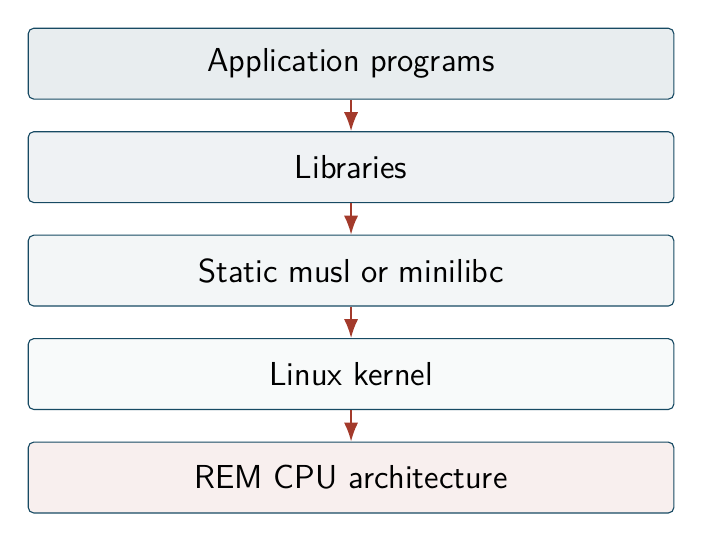
\begin{tikzpicture}[
    rembox/.style={draw=REMBlue, rounded corners=2pt, minimum width=82mm,
      minimum height=9mm, align=center, font=\sffamily\large},
    remarrow/.style={-{Latex[length=2.4mm]}, line width=0.7pt, draw=REMRed}]
    \node[rembox, fill=REMBlue!10] (app) {Application programs};
    \node[rembox, fill=REMBlue!7, below=4mm of app] (lib) {Libraries};
    \node[rembox, fill=REMBlue!5, below=4mm of lib] (libc) {Static musl or minilibc};
    \node[rembox, fill=REMBlue!3, below=4mm of libc] (kernel) {Linux kernel};
    \node[rembox, fill=REMRed!8, below=4mm of kernel] (cpu) {REM CPU architecture};
    \draw[remarrow] (app) -- (lib);
    \draw[remarrow] (lib) -- (libc);
    \draw[remarrow] (libc) -- (kernel);
    \draw[remarrow] (kernel) -- (cpu);
  \end{tikzpicture}
  \end{center}%
}
\newcommand{\REMFlowFive}[5]{%
  \begin{center}
  \begin{tikzpicture}[
    remflowbox/.style={draw=REMBlue, rounded corners=2pt, minimum width=55mm,
      minimum height=8mm, align=center, font=\sffamily\normalsize},
    remflowarrow/.style={-{Latex[length=2.2mm]}, line width=0.65pt, draw=REMRed}]
    \node[remflowbox, fill=REMBlue!7] (f1) {#1};
    \node[remflowbox, fill=REMBlue!7, below=3mm of f1] (f2) {#2};
    \node[remflowbox, fill=REMBlue!7, below=3mm of f2] (f3) {#3};
    \node[remflowbox, fill=REMBlue!7, below=3mm of f3] (f4) {#4};
    \node[remflowbox, fill=REMRed!8, below=3mm of f4] (f5) {#5};
    \draw[remflowarrow] (f1) -- (f2);
    \draw[remflowarrow] (f2) -- (f3);
    \draw[remflowarrow] (f3) -- (f4);
    \draw[remflowarrow] (f4) -- (f5);
  \end{tikzpicture}
  \end{center}%
}
\newcommand{\REMFlowThree}[3]{%
  \begin{center}
  \begin{tikzpicture}[
    remflowbox/.style={draw=REMBlue, rounded corners=2pt, minimum width=55mm,
      minimum height=8mm, align=center, font=\sffamily\normalsize},
    remflowarrow/.style={-{Latex[length=2.2mm]}, line width=0.65pt, draw=REMRed}]
    \node[remflowbox, fill=REMBlue!7] (f1) {#1};
    \node[remflowbox, fill=REMBlue!7, below=3mm of f1] (f2) {#2};
    \node[remflowbox, fill=REMRed!8, below=3mm of f2] (f3) {#3};
    \draw[remflowarrow] (f1) -- (f2);
    \draw[remflowarrow] (f2) -- (f3);
  \end{tikzpicture}
  \end{center}%
}
\newcommand{\REMFlowFour}[4]{%
  \begin{center}
  \begin{tikzpicture}[
    remflowbox/.style={draw=REMBlue, rounded corners=2pt, minimum width=55mm,
      minimum height=8mm, align=center, font=\sffamily\normalsize},
    remflowarrow/.style={-{Latex[length=2.2mm]}, line width=0.65pt, draw=REMRed}]
    \node[remflowbox, fill=REMBlue!7] (f1) {#1};
    \node[remflowbox, fill=REMBlue!7, below=3mm of f1] (f2) {#2};
    \node[remflowbox, fill=REMBlue!7, below=3mm of f2] (f3) {#3};
    \node[remflowbox, fill=REMRed!8, below=3mm of f3] (f4) {#4};
    \draw[remflowarrow] (f1) -- (f2);
    \draw[remflowarrow] (f2) -- (f3);
    \draw[remflowarrow] (f3) -- (f4);
  \end{tikzpicture}
  \end{center}%
}
\newcommand{\REMHorizontalFive}[5]{%
  \begin{center}
  \begin{tikzpicture}[
    remhbox/.style={draw=REMBlue, rounded corners=2pt, minimum width=27mm,
      minimum height=11mm, align=center, font=\sffamily\small},
    remharrow/.style={-{Latex[length=2.1mm]}, line width=0.65pt, draw=REMRed}]
    \node[remhbox, fill=REMBlue!7] (h1) {#1};
    \node[remhbox, fill=REMBlue!7, right=4mm of h1] (h2) {#2};
    \node[remhbox, fill=REMBlue!7, right=4mm of h2] (h3) {#3};
    \node[remhbox, fill=REMBlue!7, right=4mm of h3] (h4) {#4};
    \node[remhbox, fill=REMRed!8, right=4mm of h4] (h5) {#5};
    \draw[remharrow] (h1) -- (h2);
    \draw[remharrow] (h2) -- (h3);
    \draw[remharrow] (h3) -- (h4);
    \draw[remharrow] (h4) -- (h5);
  \end{tikzpicture}
  \end{center}%
}
\newcommand{\REMHorizontalThree}[3]{%
  \begin{center}
  \begin{tikzpicture}[
    remhbox/.style={draw=REMBlue, rounded corners=2pt, minimum width=39mm,
      minimum height=11mm, align=center, font=\sffamily\small},
    remharrow/.style={-{Latex[length=2.1mm]}, line width=0.65pt, draw=REMRed}]
    \node[remhbox, fill=REMBlue!7] (h1) {#1};
    \node[remhbox, fill=REMBlue!7, right=5mm of h1] (h2) {#2};
    \node[remhbox, fill=REMRed!8, right=5mm of h2] (h3) {#3};
    \draw[remharrow] (h1) -- (h2);
    \draw[remharrow] (h2) -- (h3);
  \end{tikzpicture}
  \end{center}%
}
\newcommand{\REMBytesThree}[3]{%
  \begin{center}
  \begin{tikzpicture}[
    rembyte/.style={draw=REMBlue, rounded corners=2pt, minimum width=18mm,
      minimum height=9mm, align=center, font=\ttfamily\small},
    rembytearrow/.style={-{Latex[length=2mm]}, line width=0.6pt, draw=REMRed}]
    \node[rembyte, fill=REMRed!8] (b1) {#1};
    \node[rembyte, fill=REMBlue!7, right=3mm of b1] (b2) {#2};
    \node[rembyte, fill=REMBlue!7, right=3mm of b2] (b3) {#3};
    \draw[rembytearrow] (b1) -- (b2);
    \draw[rembytearrow] (b2) -- (b3);
  \end{tikzpicture}
  \end{center}%
}
\newcommand{\REMBytesSix}[6]{%
  \begin{center}
  \begin{tikzpicture}[
    rembyte/.style={draw=REMBlue, rounded corners=2pt, minimum width=15mm,
      minimum height=9mm, align=center, font=\ttfamily\small},
    rembytearrow/.style={-{Latex[length=1.8mm]}, line width=0.55pt, draw=REMRed}]
    \node[rembyte, fill=REMRed!8] (b1) {#1};
    \node[rembyte, fill=REMBlue!7, right=2mm of b1] (b2) {#2};
    \node[rembyte, fill=REMBlue!7, right=2mm of b2] (b3) {#3};
    \node[rembyte, fill=REMBlue!7, right=2mm of b3] (b4) {#4};
    \node[rembyte, fill=REMBlue!7, right=2mm of b4] (b5) {#5};
    \node[rembyte, fill=REMBlue!7, right=2mm of b5] (b6) {#6};
    \draw[rembytearrow] (b1) -- (b2);
    \draw[rembytearrow] (b2) -- (b3);
    \draw[rembytearrow] (b3) -- (b4);
    \draw[rembytearrow] (b4) -- (b5);
    \draw[rembytearrow] (b5) -- (b6);
  \end{tikzpicture}
  \end{center}%
}
\newcommand{\REMBytesFour}[4]{%
  \begin{center}
  \begin{tikzpicture}[
    rembyte/.style={draw=REMBlue, rounded corners=2pt, minimum width=18mm,
      minimum height=9mm, align=center, font=\ttfamily\small},
    rembytearrow/.style={-{Latex[length=2mm]}, line width=0.6pt, draw=REMRed}]
    \node[rembyte, fill=REMRed!8] (b1) {#1};
    \node[rembyte, fill=REMBlue!7, right=3mm of b1] (b2) {#2};
    \node[rembyte, fill=REMBlue!7, right=3mm of b2] (b3) {#3};
    \node[rembyte, fill=REMBlue!7, right=3mm of b3] (b4) {#4};
    \draw[rembytearrow] (b1) -- (b2);
    \draw[rembytearrow] (b2) -- (b3);
    \draw[rembytearrow] (b3) -- (b4);
  \end{tikzpicture}
  \end{center}%
}
\usepackage{titlesec}
\titleformat{\chapter}[display]
  {\normalfont\sffamily\bfseries\color{REMBlue}}
  {\fontsize{13}{16}\selectfont\chaptertitlename\ \thechapter}
  {8pt}{\raggedright\fontsize{28}{32}\selectfont}
\titlespacing*{\chapter}{0pt}{-20pt}{24pt}
\titleformat{\section}
  {\normalfont\sffamily\Large\bfseries\color{REMBlue}}
  {\thesection}{0.7em}{}
\titleformat{\subsection}
  {\normalfont\sffamily\large\bfseries\color{REMRed}}
  {\thesubsection}{0.7em}{}
\usepackage{fancyhdr}
\pagestyle{fancy}
\fancyhf{}
\fancyhead[L]{\sffamily\small\nouppercase{\rightmark}}
\fancyhead[R]{\sffamily\small\thepage}
\renewcommand{\headrulewidth}{0.4pt}
\fancypagestyle{plain}{\fancyhf{}\fancyfoot[C]{\sffamily\small\thepage}\renewcommand{\headrulewidth}{0pt}}
\usepackage{booktabs}
\usepackage{longtable}
\usepackage{array}
\usepackage{etoolbox}
\AtBeginEnvironment{longtable}{\small}
\usepackage{enumitem}
\setlist{topsep=3pt,itemsep=2pt,parsep=0pt}
\usepackage{framed}
\definecolor{shadecolor}{HTML}{F4F6F7}
\usepackage{fvextra}
\RecustomVerbatimEnvironment{verbatim}{Verbatim}{breaklines=true,breakanywhere=true}
\usepackage{hyperref}
\hypersetup{colorlinks=true,linkcolor=REMBlue,urlcolor=REMRed,citecolor=REMBlue}
\usepackage{bookmark}
\setcounter{tocdepth}{0}
\renewcommand{\contentsname}{Contents}
\renewcommand{\partname}{Part}
\setlength{\emergencystretch}{3em}
\sloppy
\ifLuaTeX
  \usepackage{selnolig}  % disable illegal ligatures
\fi
\IfFileExists{bookmark.sty}{\usepackage{bookmark}}{\usepackage{hyperref}}
\IfFileExists{xurl.sty}{\usepackage{xurl}}{} % add URL line breaks if available
\urlstyle{same}
\hypersetup{
  pdftitle={Inside the REM Computer},
  pdfauthor={REM Project},
  hidelinks,
  pdfcreator={LaTeX via pandoc}}

\title{Inside the REM Computer}
\usepackage{etoolbox}
\makeatletter
\providecommand{\subtitle}[1]{% add subtitle to \maketitle
  \apptocmd{\@title}{\par {\large #1 \par}}{}{}
}
\makeatother
\subtitle{Edition 2 --- Expanded Offline Reference}
\author{REM Project}
\date{}

\begin{document}
\frontmatter
\maketitle

{
\setcounter{tocdepth}{0}
\tableofcontents
}
\mainmatter
\hypertarget{rem-quick-reference}{%
\chapter{REM Quick Reference}\label{rem-quick-reference}}

Keep this page beside the keyboard while working offline. It describes
the current MyEmulator2 target; legacy MyEmulator 1.0 uses a different
machine.

\begin{longtable}[]{@{}
  >{\raggedright\arraybackslash}p{(\columnwidth - 2\tabcolsep) * \real{0.5000}}
  >{\raggedright\arraybackslash}p{(\columnwidth - 2\tabcolsep) * \real{0.5000}}@{}}
\toprule\noalign{}
\begin{minipage}[b]{\linewidth}\raggedright
Item
\end{minipage} & \begin{minipage}[b]{\linewidth}\raggedright
Current value
\end{minipage} \\
\midrule\noalign{}
\endhead
\bottomrule\noalign{}
\endlastfoot
Architecture & MyEmulator2 / \texttt{myemulator32} \\
Word and register size & 32 bits \\
Address space & 32-bit virtual and physical addresses \\
Endianness & Little-endian \\
Instruction width & Fixed 32-bit words, 4-byte aligned \\
Page size & 4096 bytes \\
MMU & Two-level page walk: 10-bit directory, 10-bit table, 12-bit
offset \\
Privilege modes & User and Supervisor \\
General registers & \texttt{r0}--\texttt{r15}; \texttt{r0} is hardwired
zero \\
Stack and link & \texttt{r13}/\texttt{sp}, \texttt{r14}/\texttt{lr} \\
Function ABI arguments & \texttt{r1}--\texttt{r4} \\
Function ABI return & \texttt{r1} for 32-bit values \\
Linux syscall number/result & \texttt{r1} \\
Linux syscall arguments & \texttt{r2}--\texttt{r7} (up to six) \\
Executable format & ELF32 little-endian, initially static \\
Compiler/tool prefix & \texttt{myemulator2-elf-} \\
Assembler/linker & \texttt{myemulator2-elf-as},
\texttt{myemulator2-elf-ld} \\
Disassembler & \texttt{myemulator2-elf-objdump} \\
QEMU binary & \texttt{qemu-system-myemulator32} \\
QEMU machine & \texttt{myemulator32} \\
Default RAM & 16 MiB \\
Reset words & \texttt{0x400} = SSP, \texttt{0x404} = PC \\
Console MMIO & \texttt{0xF0000000}--\texttt{0xF000000F} \\
Console receive IRQ & IRQ4 \\
Timer IRQ & IRQ1 \\
\end{longtable}

The function ABI and Linux syscall ABI are separate conventions that
happen to reuse the same registers. A function receives its first
arguments in \texttt{r1}--\texttt{r4} and returns a 32-bit value in
\texttt{r1}; a syscall instead puts its number in \texttt{r1}, its
arguments in \texttt{r2}--\texttt{r7}, and its result back in
\texttt{r1}.

\hypertarget{boot}{%
\section{Boot}\label{boot}}

Current QEMU Linux path:

\begin{Shaded}
\begin{Highlighting}[]
\NormalTok{reset words}
\NormalTok{    → head.S}
\NormalTok{    → vector and stack setup}
\NormalTok{    → .bss clear}
\NormalTok{    → start\_kernel()}
\NormalTok{    → MMU, timer, console, block device}
\NormalTok{    → init}
\NormalTok{    → shell}
\end{Highlighting}
\end{Shaded}

The future RIKMON firmware path inserts firmware and an ELF loader
before the kernel. It must not be confused with the current direct QEMU
development loader.

\hypertarget{development}{%
\section{Development}\label{development}}

\begin{Shaded}
\begin{Highlighting}[]
\NormalTok{source}
\NormalTok{    → assembler}
\NormalTok{    → object file}
\NormalTok{    → linker}
\NormalTok{    → ELF32 executable}
\NormalTok{    → Linux process}
\end{Highlighting}
\end{Shaded}

\hypertarget{first-checks}{%
\section{First checks}\label{first-checks}}

\begin{Shaded}
\begin{Highlighting}[]
\ExtensionTok{./toolchain/scripts/test{-}binutils.sh}
\ExtensionTok{python3}\NormalTok{ toolchain/scripts/test{-}linux{-}process.py}
\ExtensionTok{python3}\NormalTok{ toolchain/scripts/test{-}linux{-}minilibc.py}
\end{Highlighting}
\end{Shaded}

\begin{center}\rule{0.5\linewidth}{0.5pt}\end{center}

\hypertarget{rem-reference-alignment-second-pass-notes}{%
\chapter{REM Reference Alignment --- Second Pass
Notes}\label{rem-reference-alignment-second-pass-notes}}

This edition aligns the book against the current REM reference manuals.

\hypertarget{terminology-and-status-corrections}{%
\section{Terminology and status
corrections}\label{terminology-and-status-corrections}}

The following distinctions are enforced:

\begin{itemize}
\tightlist
\item
  REM / MyEmulator2 refers to the current 32-bit target, not the legacy
  MyEmulator firmware target.
\item
  Implemented features are separated from planned features.
\item
  Host QEMU validation and Android Fold deployment validation are
  treated separately.
\item
  Toolchain availability does not imply a complete in-guest development
  environment.
\end{itemize}

\hypertarget{current-implementation-baseline}{%
\section{Current implementation
baseline}\label{current-implementation-baseline}}

The reference manual defines the current target as:

\begin{itemize}
\tightlist
\item
  32-bit little-endian byte-addressed CPU.
\item
  Fixed-width 32-bit instructions.
\item
  ELF32 little-endian static executable workflow.
\item
  GNU assembler/linker support.
\item
  GCC integer and soft-float backend support.
\item
  Linux entry, user ELF loading and process lifecycle support.
\end{itemize}

\hypertarget{known-boundaries-to-preserve}{%
\section{Known boundaries to
preserve}\label{known-boundaries-to-preserve}}

The book must not imply that the following are complete:

\begin{itemize}
\tightlist
\item
  full Linux syscall coverage;
\item
  dynamic linking;
\item
  shared libraries;
\item
  dynamic TLS;
\item
  complete libc/POSIX coverage;
\item
  final userspace ABI details;
\item
  networking;
\item
  complete in-guest package/development environment.
\end{itemize}

\hypertarget{fold-deployment-wording}{%
\section{Fold deployment wording}\label{fold-deployment-wording}}

Galaxy Fold execution remains a deployment target requiring device
validation. Host QEMU success is not equivalent to phone execution.

\begin{center}\rule{0.5\linewidth}{0.5pt}\end{center}

\hypertarget{rem-reality-table}{%
\chapter{REM Reality Table}\label{rem-reality-table}}

\begin{longtable}[]{@{}
  >{\raggedright\arraybackslash}p{(\columnwidth - 2\tabcolsep) * \real{0.4861}}
  >{\raggedright\arraybackslash}p{(\columnwidth - 2\tabcolsep) * \real{0.4861}}@{}}
\toprule\noalign{}
\begin{minipage}[b]{\linewidth}\raggedright
Area
\end{minipage} & \begin{minipage}[b]{\linewidth}\raggedright
Current status
\end{minipage} \\
\midrule\noalign{}
\endhead
\bottomrule\noalign{}
\endlastfoot
CPU architecture & Implemented and under active development \\
Linux kernel support & Implemented/tested according to project status \\
Toolchain & Available in the REM environment \\
Host QEMU & Development and regression environment \\
Galaxy Fold deployment & Requires device validation \\
Native applications & Development phase \\
REMEDIT & Example development environment project \\
\end{longtable}

This review draft distinguishes completed capabilities, tested
capabilities, and planned work.

\begin{center}\rule{0.5\linewidth}{0.5pt}\end{center}

\hypertarget{canonical-rem-conventions-for-the-examples}{%
\chapter{Canonical REM conventions for the
examples}\label{canonical-rem-conventions-for-the-examples}}

The detailed chapters below retain the original book's worked examples,
but current REM conventions take precedence wherever an older example
uses different names or registers.

The target is a 32-bit little-endian architecture using ELF32 static
executables. The ordinary function ABI uses \texttt{r0} as constant
zero, \texttt{r1}--\texttt{r4} for arguments, \texttt{r1} for a 32-bit
return value, \texttt{r13} as the stack pointer, and \texttt{r14} as the
link register. The stack is downward growing and 16-byte aligned at call
boundaries.

Linux syscalls use a separate userspace convention: \texttt{r1} contains
the syscall number and return value, while arguments use
\texttt{r2}--\texttt{r7}. The currently exercised process path uses
\texttt{clone}, \texttt{execve}, and \texttt{wait4}; the complete
syscall ABI is still under development. Applications using the hosted C
environment should use the project's statically linked MyEmulator2 musl
toolchain. Dynamic linking and complete POSIX coverage remain future
work.

When a chapter says a facility is planned, that does not make it a
requirement for the first REMEDIT milestone. Host QEMU validation and
Galaxy Fold deployment must be recorded separately.

\begin{center}\rule{0.5\linewidth}{0.5pt}\end{center}

\hypertarget{how-to-use-this-offline-edition}{%
\chapter{How to use this offline
edition}\label{how-to-use-this-offline-edition}}

This book contains examples from earlier REM development stages. Before
copying an example, identify its target:

\begin{longtable}[]{@{}
  >{\raggedright\arraybackslash}p{(\columnwidth - 2\tabcolsep) * \real{0.5000}}
  >{\raggedright\arraybackslash}p{(\columnwidth - 2\tabcolsep) * \real{0.5000}}@{}}
\toprule\noalign{}
\begin{minipage}[b]{\linewidth}\raggedright
Target
\end{minipage} & \begin{minipage}[b]{\linewidth}\raggedright
Tools and execution model
\end{minipage} \\
\midrule\noalign{}
\endhead
\bottomrule\noalign{}
\endlastfoot
Legacy MyEmulator 1.0 & \texttt{tools/myasm}, raw firmware image,
separate 8-bit/16-bit architecture \\
MyEmulator2 bare metal & \texttt{myemulator2-elf-as},
\texttt{myemulator2-elf-ld}, ELF32 or derived raw image \\
MyEmulator2 Linux & MyEmulator2 GCC/musl or minilibc, Linux ELF, QEMU
Linux machine \\
\end{longtable}

The current MyEmulator2 assembler uses GNU syntax: lowercase mnemonics
are canonical, registers are \texttt{r0} through \texttt{r15}, memory
operands use \texttt{displacement(base)}, and \texttt{\#} begins a
comment. Older examples using names such as \texttt{MOV}, \texttt{LOAD},
\texttt{STORE}, or bracketed addresses are explanatory pseudocode unless
the surrounding chapter identifies a legacy target.

The authoritative local references are:

\begin{Shaded}
\begin{Highlighting}[]
\NormalTok{docs/MYEMULATOR2\_ASSEMBLY\_PROGRAMMING\_MANUAL.md}
\NormalTok{docs/MYEMULATOR\_2\_ABI.md}
\NormalTok{docs/MYEMULATOR\_2\_ARCHITECTURE.md}
\NormalTok{docs/MYEMULATOR\_2\_LINUX\_PORT.md}
\NormalTok{toolchain/README.md}
\NormalTok{docs/console.md}
\NormalTok{android/README.md}
\end{Highlighting}
\end{Shaded}

When a result matters, record the command used, the target being tested,
and whether the result came from host QEMU or a physical Fold.

This offline edition has three kinds of material. The main chapters are
\textbf{conceptual}: they explain the design and the decisions behind
it. Part VIII contains \textbf{worked programs}: small executable
bridges for the platform, ABI, terminal, and toolchain boundaries. The
appendices are \textbf{reference}: condensed commands, constants,
tables, and checklists for later lookup.

Status labels are used where a reader could otherwise mistake a design
for a current facility: \textbf{{[}IMPLEMENTED{]}} means present in the
repository, \textbf{{[}TESTED{]}} means covered by a named regression or
reproducible check, \textbf{{[}EXPERIMENTAL{]}} means present but liable
to change, \textbf{{[}PLANNED{]}} means a design or future task, and
\textbf{{[}LEGACY{]}} identifies the older target or syntax.

\hypertarget{remedits-role}{%
\section{REMEDIT's role}\label{remedits-role}}

REMEDIT is the running engineering project through which the techniques
in this book are applied; it is not a finished application for the
reader to reproduce line by line. The book supplies the REM-specific
mechanisms, interfaces, contracts, and worked examples needed to build
it. Decisions about the editor's application logic---such as buffer
representation, undo records, lexer states, and command policy---remain
the reader's work. When a problem is caused by REM's ISA, ABI, terminal,
kernel, toolchain, or QEMU, the book aims to provide the information
needed to solve it offline. When it is an editor design decision, the
problem is part of the project.

\begin{center}\rule{0.5\linewidth}{0.5pt}\end{center}

\hypertarget{historical-development-path}{%
\chapter{Historical development
path}\label{historical-development-path}}

REM did not begin as a finished 32-bit Linux architecture. Its
development path matters because the repository still contains tools and
examples from each stage:

\textbf{Flow:} Python 8-bit computer → emulated CPU and firmware →
MyEmulator2 32-bit QEMU target → ELF32 assembler, linker, and GCC →
Linux kernel and userspace bring-up

Historical examples are useful for understanding why a subsystem exists,
but they are not automatically current implementation instructions. The
target table and the legacy conversion appendix identify which examples
can be assembled for MyEmulator2 today.

\begin{center}\rule{0.5\linewidth}{0.5pt}\end{center}

\part{Part 0 — Architecture and Platform Reference}

The chapters that follow teach software construction. This part fixes
the machine model those chapters assume. It is a map of the layers, not
a second instruction manual. The architecture and assembly manuals
remain the final authority for encoding and instruction behavior.

\hypertarget{rem-architecture-reference}{%
\chapter{REM Architecture Reference}\label{rem-architecture-reference}}

MyEmulator2 is a 32-bit, little-endian, byte-addressed architecture.
Values, addresses, and instruction words are 32 bits. Instructions are
fixed-width, stored little-endian, and 4-byte aligned. Sequential
execution advances the program counter by four.

\hypertarget{programmer-visible-state}{%
\section{Programmer-visible state}\label{programmer-visible-state}}

\begin{longtable}[]{@{}ll@{}}
\toprule\noalign{}
State & Meaning \\
\midrule\noalign{}
\endhead
\bottomrule\noalign{}
\endlastfoot
\texttt{r0} / \texttt{zero} & hardwired zero; writes are discarded \\
\texttt{r1}--\texttt{r12} & general registers \\
\texttt{r13} / \texttt{sp} & banked user or supervisor stack pointer \\
\texttt{r14} / \texttt{lr} & link register used by \texttt{jal} \\
\texttt{r15} & general temporary register \\
\texttt{PC} & program counter \\
\texttt{SR} & carry, overflow, interrupt priority, and privilege
state \\
\end{longtable}

There are User and Supervisor modes. \texttt{SR.S} selects the mode.
\texttt{r13} refers to the user stack pointer in User mode and the
supervisor stack pointer in Supervisor mode. Supervisor software can
access both through system-register operations; User software cannot
directly access the supervisor stack.

The initial function ABI uses \texttt{r1}--\texttt{r4} for the first
four arguments, \texttt{r1} for a 32-bit return value,
\texttt{r5}--\texttt{r12} as callee-saved registers, \texttt{r15} as a
caller-saved temporary, and \texttt{r14} as the link register. The stack
grows downward, is 16-byte aligned at call boundaries, and has no red
zone.

\hypertarget{exceptions-and-interrupts}{%
\section{Exceptions and interrupts}\label{exceptions-and-interrupts}}

The CPU has vectors for illegal instructions, privilege violations,
alignment faults, page-not-present and protection faults, divide by
zero, arithmetic overflow, system calls, breakpoints, NMI, double fault,
and IRQ1--IRQ7. Hardware builds an exception frame on the supervisor
stack. Linux expands that into its software \texttt{pt\_regs} frame
before calling C code. General registers are not automatically preserved
by hardware handlers.

The timer uses IRQ1. The current console receive path uses IRQ4.
Interrupt priority is controlled by \texttt{SR.IPL}; priority 7 masks
ordinary IRQs.

\hypertarget{mmu-model}{%
\section{MMU model}\label{mmu-model}}

With \texttt{MMCR.EN=0}, virtual addresses are physical addresses and
page permissions do not apply. With the MMU enabled, translation uses a
two-level, 4 KiB page walk:

\begin{Shaded}
\begin{Highlighting}[]
\NormalTok{virtual address}
\NormalTok{31             22 21             12 11                0}
\NormalTok{+{-}{-}{-}{-}{-}{-}{-}{-}{-}{-}{-}{-}{-}{-}{-}{-}+{-}{-}{-}{-}{-}{-}{-}{-}{-}{-}{-}{-}{-}{-}{-}{-}+{-}{-}{-}{-}{-}{-}{-}{-}{-}{-}{-}{-}{-}{-}{-}{-}{-}{-}{-}+}
\NormalTok{| page directory | page table     | page offset       |}
\NormalTok{| index (10)     | index (10)     | (12)              |}
\NormalTok{+{-}{-}{-}{-}{-}{-}{-}{-}{-}{-}{-}{-}{-}{-}{-}{-}+{-}{-}{-}{-}{-}{-}{-}{-}{-}{-}{-}{-}{-}{-}{-}{-}+{-}{-}{-}{-}{-}{-}{-}{-}{-}{-}{-}{-}{-}{-}{-}{-}{-}{-}{-}+}
\NormalTok{        |                |}
\NormalTok{        v                v}
\NormalTok{     PDE table  {-}{-}{-}{-}{-}{-}\textgreater{} PTE {-}{-}{-}{-}{-}{-}\textgreater{} physical 4 KiB page}
\end{Highlighting}
\end{Shaded}

\texttt{PTBR} points to a physical, 4 KiB-aligned 1024-entry page
directory. PDE and PTE entries carry present, user, read, write,
execute, accessed, and dirty bits. Effective permissions are the
intersection of the directory and table entries. A missing entry
produces a not-present fault; an insufficient permission produces a
protection fault. The MMU sets accessed and dirty bits on successful
accesses. There are no huge pages or legacy paging modes.

MyEmulator2 is strongly ordered. Ordinary loads and stores become
visible in program order. \texttt{CAS} is a naturally aligned, fully
ordered 32-bit atomic compare-and-swap. There are no fence instructions
in the current ISA.

\hypertarget{elf-and-deployment-boundary}{%
\section{ELF and deployment
boundary}\label{elf-and-deployment-boundary}}

The canonical object and executable format is ELF32 little-endian with
the project-local provisional machine identifier. Static executables are
the initial ABI. Dynamic linking, shared libraries, dynamic TLS, and
final aggregate/varargs ABI rules remain future work. A raw image
produced by \texttt{objcopy\ -O\ binary} is a derived deployment
artifact; it does not contain the ELF entry point.

\hypertarget{rem-linux-boot-sequence}{%
\chapter{REM Linux Boot Sequence}\label{rem-linux-boot-sequence}}

The current Linux boot path begins with QEMU publishing the initial
stack and program counter through physical reset words at \texttt{0x400}
and \texttt{0x404}. The CPU starts in Supervisor mode with translation
disabled and fetches the first instruction physically.

The tracked sequence is:

\begin{Shaded}
\begin{Highlighting}[]
\NormalTok{reset words at 0x400 / 0x404}
\NormalTok{        |}
\NormalTok{        v}
\NormalTok{linux/arch/myemulator2/kernel/head.S:\_start}
\NormalTok{        |}
\NormalTok{        +{-}{-} select the linked Linux stack}
\NormalTok{        +{-}{-} install the vector table in VBR}
\NormalTok{        +{-}{-} clear .bss}
\NormalTok{        v}
\NormalTok{myemulator2\_start\_kernel()}
\NormalTok{        |}
\NormalTok{        v}
\NormalTok{start\_kernel()}
\NormalTok{        |}
\NormalTok{        +{-}{-} describe RAM to memblock}
\NormalTok{        +{-}{-} construct page tables and enable the MMU}
\NormalTok{        +{-}{-} register timer, block, and serial console}
\NormalTok{        +{-}{-} create the initial userspace process}
\NormalTok{        v}
\NormalTok{/sbin/init and the guest shell}
\end{Highlighting}
\end{Shaded}

The kernel is linked with a 4 KiB page size. The current machine
normally has 16 MiB of RAM, while the kernel reads the configured RAM
extent from the boot descriptor at \texttt{0x408}. The exact initramfs,
root filesystem, and command line are deployment inputs, not CPU reset
behavior.

\hypertarget{isa-platform-kernel-and-userspace}{%
\chapter{ISA, Platform, Kernel, and
Userspace}\label{isa-platform-kernel-and-userspace}}

Keep these boundaries separate:

\begin{Shaded}
\begin{Highlighting}[]
\NormalTok{+{-}{-}{-}{-}{-}{-}{-}{-}{-}{-}{-}{-}{-}{-}{-}{-}{-}{-}{-}{-}{-}{-}{-}{-}{-}{-}{-}{-}{-}{-}{-}+}
\NormalTok{| REM applications              |}
\NormalTok{+{-}{-}{-}{-}{-}{-}{-}{-}{-}{-}{-}{-}{-}{-}{-}{-}{-}{-}{-}{-}{-}{-}{-}{-}{-}{-}{-}{-}{-}{-}{-}+}
\NormalTok{| static musl / minilibc        |}
\NormalTok{+{-}{-}{-}{-}{-}{-}{-}{-}{-}{-}{-}{-}{-}{-}{-}{-}{-}{-}{-}{-}{-}{-}{-}{-}{-}{-}{-}{-}{-}{-}{-}+}
\NormalTok{| Linux syscall and tty ABI     |}
\NormalTok{+{-}{-}{-}{-}{-}{-}{-}{-}{-}{-}{-}{-}{-}{-}{-}{-}{-}{-}{-}{-}{-}{-}{-}{-}{-}{-}{-}{-}{-}{-}{-}+}
\NormalTok{| Linux kernel                  |}
\NormalTok{+{-}{-}{-}{-}{-}{-}{-}{-}{-}{-}{-}{-}{-}{-}{-}{-}{-}{-}{-}{-}{-}{-}{-}{-}{-}{-}{-}{-}{-}{-}{-}+}
\NormalTok{| REM platform: console, timer,|}
\NormalTok{| block device, QEMU machine    |}
\NormalTok{+{-}{-}{-}{-}{-}{-}{-}{-}{-}{-}{-}{-}{-}{-}{-}{-}{-}{-}{-}{-}{-}{-}{-}{-}{-}{-}{-}{-}{-}{-}{-}+}
\NormalTok{| MyEmulator2 CPU ISA and MMU   |}
\NormalTok{+{-}{-}{-}{-}{-}{-}{-}{-}{-}{-}{-}{-}{-}{-}{-}{-}{-}{-}{-}{-}{-}{-}{-}{-}{-}{-}{-}{-}{-}{-}{-}+}
\end{Highlighting}
\end{Shaded}

An instruction belongs to the ISA. The \texttt{0xF0000000} console
belongs to the platform. \texttt{termios}, ELF process startup, and
syscall numbers belong to Linux userspace. QEMU emulates the platform;
it does not turn an unimplemented guest feature into an ISA feature.

\hypertarget{what-is-implemented-planned-or-unspecified}{%
\chapter{What Is Implemented, Planned, or
Unspecified}\label{what-is-implemented-planned-or-unspecified}}

The current implementation includes the 32-bit CPU/MMU, exception
integration, ELF32 static toolchain, GCC integer and soft-float backend,
Linux entry and user ELF loading, basic process lifecycle, serial
console, timer, and ext4 block-device work. The syscall table, signals,
complete libc/POSIX behavior, dynamic linking, networking, and a stable
userspace ABI remain incomplete.

SMP is disabled in the current Linux configuration. USB, sound,
networking, and virtual graphics are disabled in the current
Android/QEMU deployment. Features not mentioned in the architecture
contract should be treated as unspecified rather than assumed absent or
present.

\hypertarget{developer-journeys}{%
\chapter{Developer Journeys}\label{developer-journeys}}

\hypertarget{bare-metal-assembly}{%
\section{Bare-metal assembly}\label{bare-metal-assembly}}

\begin{enumerate}
\def\labelenumi{\arabic{enumi}.}
\tightlist
\item
  Build the \texttt{myemulator2-elf} tools.
\item
  Assemble and link an ELF32 program.
\item
  Inspect it with \texttt{readelf} and \texttt{objdump}.
\item
  Run it under the MyEmulator2 QEMU machine.
\item
  Add a focused regression test.
\end{enumerate}

\hypertarget{linux-application-development}{%
\section{Linux application
development}\label{linux-application-development}}

\begin{enumerate}
\def\labelenumi{\arabic{enumi}.}
\tightlist
\item
  Build or install the MyEmulator2 GCC and static musl/minilibc path.
\item
  Produce a static ELF executable.
\item
  Boot the verified Linux kernel and root filesystem.
\item
  Exercise the program under host QEMU.
\item
  Repeat the deployment and persistence checks on the Fold separately.
\end{enumerate}

The smallest maintained Linux C milestone is the minilibc regression. It
builds \texttt{toolchain/examples/linux-minilibc.c} with the target
compiler, links the REM startup and syscall wrappers, boots a disposable
initramfs, and expects the strings \texttt{C\ minilibc\ reached} and
\texttt{C\ syscall\ wrappers\ reached}. Run it with:

\begin{Shaded}
\begin{Highlighting}[]
\ExtensionTok{python3}\NormalTok{ toolchain/scripts/test{-}linux{-}minilibc.py}
\end{Highlighting}
\end{Shaded}

This is the offline equivalent of a first ``Hello Linux'' program. The
larger static musl regression uses
\texttt{toolchain/examples/linux-libc-regression.c} and exercises files,
allocation, strings, time, and platform reporting.

\hypertarget{emulator-and-kernel-development}{%
\section{Emulator and kernel
development}\label{emulator-and-kernel-development}}

\begin{enumerate}
\def\labelenumi{\arabic{enumi}.}
\tightlist
\item
  Change one ISA, MMU, device, or kernel component.
\item
  Run the narrowest existing regression.
\item
  Run the CPU/system or Linux process suite.
\item
  Inspect QEMU traces and structured debug state when needed.
\item
  Record whether the result is host-only, guest-tested, or phone-tested.
\end{enumerate}

\begin{center}\rule{0.5\linewidth}{0.5pt}\end{center}

\begin{center}\rule{0.5\linewidth}{0.5pt}\end{center}

\hypertarget{preface}{%
\chapter{Preface}\label{preface}}

\hypertarget{why-this-book-exists}{%
\section{Why this book exists}\label{why-this-book-exists}}

When building a new computer architecture, there is a natural
progression.

The first milestone is making the processor execute instructions.

The second milestone is making the processor run an operating system.

The third milestone is making the machine useful.

That final step is where software developers enter the picture.

A CPU manual can tell you everything about the machine:

\begin{itemize}
\tightlist
\item
  the registers
\item
  the instruction set
\item
  the memory model
\item
  the ABI
\item
  the assembler syntax
\item
  the system call interface
\end{itemize}

Those documents answer the question:

\begin{quote}
``What can this computer do?''
\end{quote}

They do not answer the question:

\begin{quote}
``How do I build software for this computer?''
\end{quote}

That is the purpose of this book.

\begin{center}\rule{0.5\linewidth}{0.5pt}\end{center}

\hypertarget{the-difference-between-a-cpu-manual-and-a-programming-environment}{%
\section{The difference between a CPU manual and a programming
environment}\label{the-difference-between-a-cpu-manual-and-a-programming-environment}}

A CPU manual is written from the perspective of the hardware.

It describes the machine as the processor sees it:

\begin{verbatim}

Registers
Instructions
Memory
Exceptions
Interrupts
System calls
\end{verbatim}

A programmer thinks differently.

A programmer needs to know:

\begin{verbatim}

How do I structure a program?

How do I debug it?

How do I handle input?

How do I display output?

How do I organise a large assembly project?

How do I build tools that make the next program easier?
\end{verbatim}

There is a large gap between these two views.

A processor can execute instructions perfectly and still be a difficult
computer to program.

The difference between an interesting CPU design and a usable computer
is the software environment built around it.

This book exists to document that environment.

\begin{center}\rule{0.5\linewidth}{0.5pt}\end{center}

\hypertarget{what-rem-already-provides}{%
\section{What REM already provides}\label{what-rem-already-provides}}

REM has already passed the stage where every program must directly
control the hardware.

The original challenge was proving that a new instruction set
architecture could support a modern software environment.

The result is not a toy interpreter or a limited demonstration system.

REM provides a growing Linux application environment, with the verified
subset identified in the Linux port documentation:

\textbf{Flow:} Application programs → Libraries → static musl or
minilibc → Linux kernel → REM CPU architecture

The programmer working on REM is not starting from bare metal.

The machine already provides:

\begin{itemize}
\tightlist
\item
  a Linux kernel environment
\item
  an executable format
\item
  an assembler and linker toolchain
\item
  a static C runtime path
\item
  selected standard-library functionality
\item
  the tested subset of Linux process and file operations
\end{itemize}

This changes the nature of the problem.

The question is no longer:

\begin{quote}
``Can REM run code?''
\end{quote}

The question becomes:

\begin{quote}
``How do we write good software on REM?''
\end{quote}

\begin{center}\rule{0.5\linewidth}{0.5pt}\end{center}

\hypertarget{what-the-application-programmer-still-needs-to-build}{%
\section{What the application programmer still needs to
build}\label{what-the-application-programmer-still-needs-to-build}}

The existing REM documentation explains the machine.

This book explains the software engineering required to use that machine
effectively.

The missing knowledge is the practical layer:

\begin{itemize}
\tightlist
\item
  how to organise a large assembly project
\item
  how to divide software into modules
\item
  how to test low-level components
\item
  how to debug failures
\item
  how to interact with the terminal
\item
  how editors and development tools are actually built
\item
  how to create software that makes future software easier to write
\end{itemize}

A programmer who has only the instruction manual can write a program.

A programmer with this book can build an environment.

\begin{center}\rule{0.5\linewidth}{0.5pt}\end{center}

\hypertarget{the-intended-reader}{%
\section{The intended reader}\label{the-intended-reader}}

This book assumes that the reader already understands programming.

It is not an introduction to:

\begin{itemize}
\tightlist
\item
  variables
\item
  loops
\item
  pointers
\item
  basic C syntax
\item
  assembly language concepts
\item
  Makefiles
\item
  compilation
\end{itemize}

The intended reader is someone who has written software before and is
comfortable looking at assembly code.

However, REM introduces areas where even an experienced programmer may
need guidance.

For example:

A programmer who has used \texttt{ncurses} may know how to create a
terminal application:

\begin{Shaded}
\begin{Highlighting}[]
\NormalTok{move}\OperatorTok{(}\DecValTok{10}\OperatorTok{,}\DecValTok{20}\OperatorTok{);}
\NormalTok{printw}\OperatorTok{(}\StringTok{"Hello"}\OperatorTok{);}
\NormalTok{refresh}\OperatorTok{();}
\end{Highlighting}
\end{Shaded}

But ncurses hides a significant amount of machinery:

\begin{itemize}
\tightlist
\item
  terminal modes
\item
  cursor positioning
\item
  escape sequences
\item
  keyboard decoding
\item
  screen updates
\end{itemize}

When writing a native REM application, some of those layers become
visible.

This book explains those layers.

\begin{center}\rule{0.5\linewidth}{0.5pt}\end{center}

\hypertarget{how-to-use-this-book-alongside-the-rem-manuals}{%
\section{How to use this book alongside the REM
manuals}\label{how-to-use-this-book-alongside-the-rem-manuals}}

The REM documentation is divided by purpose.

The architecture documentation remains the authoritative source for:

\begin{itemize}
\tightlist
\item
  instruction behaviour
\item
  register definitions
\item
  ABI details
\item
  assembler syntax
\item
  system calls
\item
  CPU operation
\end{itemize}

This book deliberately does not duplicate that information.

Instead, it assumes those manuals are available and concentrates on the
engineering decisions that happen above them.

A useful mental model is:

\begin{verbatim}
REM Architecture Manual
        |
        |  "How does the machine work?"
        |
        v
Inside the REM Computer
        |
        |  "How do I build useful software?"
        |
        v
Applications and tools
\end{verbatim}

When a question is about an instruction, consult the architecture
documentation.

When a question is:

\begin{quote}
``How should I design this program?''
\end{quote}

or:

\begin{quote}
``How do I build a tool that other programmers can use?''
\end{quote}

this book is the guide.

\begin{center}\rule{0.5\linewidth}{0.5pt}\end{center}

\hypertarget{the-philosophy-of-this-book}{%
\section{The philosophy of this
book}\label{the-philosophy-of-this-book}}

The examples in this book follow one principle:

Build small things that prove assumptions.

A common mistake in systems programming is to begin with the final
application.

For example, when building a text editor, it is tempting to immediately
write:

\begin{itemize}
\tightlist
\item
  the screen handling
\item
  the menus
\item
  the file system
\item
  the command system
\end{itemize}

That creates a large number of unknowns.

A better approach is:

\begin{verbatim}
Terminal test
      |
Keyboard test
      |
File test
      |
Buffer test
      |
Editor
\end{verbatim}

Each layer proves the layer beneath it.

This approach is slower for the first hour and much faster over the
lifetime of the project.

\begin{center}\rule{0.5\linewidth}{0.5pt}\end{center}

\hypertarget{the-example-project}{%
\section{The example project}\label{the-example-project}}

The running example throughout this book is REMEDIT: a native REM text
editor and development environment.

The choice of an editor is deliberate.

A text editor touches almost every important area of systems
programming:

\begin{itemize}
\tightlist
\item
  terminal handling
\item
  keyboard input
\item
  memory management
\item
  file I/O
\item
  data structures
\item
  rendering
\item
  process control
\item
  integration with the toolchain
\end{itemize}

Building an editor is not about creating another text editor.

It is about creating a practical test of whether REM is a usable
computer platform.

By the end of this book, the goal is not simply to have an editor.

The goal is to have a development environment that makes building the
next REM application easier.

\part{Part I — Becoming Productive on REM}

\hypertarget{chapter-1-welcome-to-rem-application-development}{%
\chapter{Chapter 1 --- Welcome to REM Application
Development}\label{chapter-1-welcome-to-rem-application-development}}

\hypertarget{the-machine-is-finished-now-build-the-ecosystem}{%
\section{1.1 The machine is finished; now build the
ecosystem}\label{the-machine-is-finished-now-build-the-ecosystem}}

There is a particular point in the life of any computer architecture
where the nature of the work changes.

At the beginning, everything is about the processor.

Can it execute instructions?

Can it access memory?

Can it handle exceptions?

Can it boot an operating system?

These are architecture questions.

They are the questions answered by the REM architecture documentation.

However, once a processor can execute a real operating system and run
normal programs, the interesting problems move upward.

The question changes from:

\begin{quote}
``Can this CPU run software?''
\end{quote}

to:

\begin{quote}
``Can a programmer comfortably build software for this CPU?''
\end{quote}

This is the point where REM has arrived.

The CPU is no longer the project.

The computer is the project.

A useful way to think about the REM software stack is:

\REMSoftwareStack

Each layer exists to make the layer above it easier to use.

The CPU provides the fundamental operations.

The kernel provides the operating environment.

The C library provides common functionality.

Applications build on top of those foundations.

A programmer writing REM applications should normally think at the top
of this stack.

You are not writing every instruction that controls the machine.

You are writing software that uses the machine.

That distinction is important.

\begin{center}\rule{0.5\linewidth}{0.5pt}\end{center}

\hypertarget{moving-from-cpu-development-to-application-development}{%
\section{1.2 Moving from CPU development to application
development}\label{moving-from-cpu-development-to-application-development}}

When designing a processor, it is natural to focus on the lowest level.

You think about:

\begin{itemize}
\tightlist
\item
  registers
\item
  instruction formats
\item
  memory access
\item
  pipeline behaviour
\item
  exceptions
\item
  privilege levels
\end{itemize}

These are the things that make a processor a processor.

Application development has a different set of concerns.

A programmer writing a text editor, compiler, database, or network
service is more concerned with:

\begin{itemize}
\tightlist
\item
  How do I organise this program?
\item
  How do I handle input?
\item
  How do I store data?
\item
  How do I recover from errors?
\item
  How do I debug failures?
\item
  How do I make this maintainable?
\end{itemize}

The processor matters, but it becomes the foundation rather than the
focus.

A useful comparison is building a house.

The CPU is the foundation.

The operating system is the structure.

The libraries are the utilities.

The application is the house.

A good foundation is essential, but nobody lives in a foundation.

\begin{center}\rule{0.5\linewidth}{0.5pt}\end{center}

\hypertarget{what-you-already-have}{%
\section{1.3 What you already have}\label{what-you-already-have}}

One of the easiest mistakes when working with a new architecture is
assuming that everything must be rebuilt.

That is true when bringing up a bare processor.

It is not true when building applications on a working Linux platform.

REM already has the important components required for normal software
development.

\begin{center}\rule{0.5\linewidth}{0.5pt}\end{center}

\hypertarget{the-assembler-gas}{%
\section{The assembler: GAS}\label{the-assembler-gas}}

The GNU assembler is the first step in the software creation process.

It converts human-readable assembly source:

\begin{verbatim}

source.s
\end{verbatim}

into machine code contained inside an object file:

\begin{verbatim}

source.o
\end{verbatim}

The assembler understands:

\begin{itemize}
\tightlist
\item
  REM instruction syntax
\item
  labels
\item
  sections
\item
  symbols
\item
  relocations
\end{itemize}

The assembler answers the question:

\begin{quote}
``How do I express a program in the REM instruction set?''
\end{quote}

\begin{center}\rule{0.5\linewidth}{0.5pt}\end{center}

\hypertarget{the-linker-ld}{%
\section{The linker: LD}\label{the-linker-ld}}

The assembler does not create the final executable.

It creates pieces.

The linker combines those pieces.

For example:

\textbf{Flow:}
main.o\textbackslash terminal.o\textbackslash buffer.o\textbackslash library.o
→ linker → REM executable

The linker resolves:

\begin{itemize}
\tightlist
\item
  symbol references
\item
  memory layout
\item
  executable format
\item
  library dependencies
\end{itemize}

Understanding the linker is one of the major steps from writing small
programs to building real applications.

\begin{center}\rule{0.5\linewidth}{0.5pt}\end{center}

\hypertarget{gcc-backend}{%
\section{GCC backend}\label{gcc-backend}}

Although this book focuses heavily on assembly programming, REM also has
compiler support.

The compiler provides another way of producing code for REM.

This matters because not every problem benefits from assembly.

A practical systems programmer chooses the right tool.

Assembly is excellent for:

\begin{itemize}
\tightlist
\item
  understanding the architecture
\item
  performance-critical routines
\item
  hardware interfaces
\item
  low-level experimentation
\end{itemize}

A higher-level language is often better for:

\begin{itemize}
\tightlist
\item
  large amounts of application logic
\item
  data processing
\item
  user interfaces
\item
  complex algorithms
\end{itemize}

A computer architecture becomes much more useful when it supports
multiple ways of creating software.

\begin{center}\rule{0.5\linewidth}{0.5pt}\end{center}

\hypertarget{libgcc}{%
\section{libgcc}\label{libgcc}}

The compiler runtime provides low-level support functions required by
generated code.

These routines handle operations that may not directly exist as single
CPU instructions.

Examples include:

\begin{itemize}
\tightlist
\item
  arithmetic helpers
\item
  compiler-generated support routines
\item
  runtime operations
\end{itemize}

The important point is that application developers do not normally write
these themselves.

They are part of the platform.

\begin{center}\rule{0.5\linewidth}{0.5pt}\end{center}

\hypertarget{musl-libc}{%
\section{musl libc}\label{musl-libc}}

The C library is where the Linux programming environment becomes
familiar.

Instead of manually implementing common operations, applications can use
standard interfaces.

Examples:

Memory:

\begin{Shaded}
\begin{Highlighting}[]
\NormalTok{malloc}\OperatorTok{()}
\NormalTok{free}\OperatorTok{()}
\NormalTok{memcpy}\OperatorTok{()}
\end{Highlighting}
\end{Shaded}

Files:

\begin{Shaded}
\begin{Highlighting}[]
\NormalTok{open}\OperatorTok{()}
\NormalTok{read}\OperatorTok{()}
\NormalTok{write}\OperatorTok{()}
\NormalTok{close}\OperatorTok{()}
\end{Highlighting}
\end{Shaded}

Output:

\begin{Shaded}
\begin{Highlighting}[]
\NormalTok{printf}\OperatorTok{()}
\end{Highlighting}
\end{Shaded}

Processes:

\begin{Shaded}
\begin{Highlighting}[]
\NormalTok{clone}\OperatorTok{()}
\NormalTok{execve}\OperatorTok{()}
\NormalTok{wait4}\OperatorTok{()}
\end{Highlighting}
\end{Shaded}

The verified static musl/minilibc environment exposes the supported
subset of these operations. The names and availability of other POSIX
interfaces must be checked against the current Linux port.

The existence of a hosted C path is a major milestone for REM.

It means selected applications can use familiar Unix interfaces while
the remaining syscall, libc, signal, and userspace ABI work continues.

\begin{center}\rule{0.5\linewidth}{0.5pt}\end{center}

\hypertarget{busybox-and-the-shell-environment}{%
\section{BusyBox and the shell
environment}\label{busybox-and-the-shell-environment}}

A computer becomes useful when it can run programs that help create
other programs.

The shell provides the interactive environment:

\begin{verbatim}
$ command
\end{verbatim}

Utilities provide the basic tools:

\begin{itemize}
\tightlist
\item
  file management
\item
  text processing
\item
  scripting support
\item
  system inspection
\end{itemize}

The exact set of available utilities may change as the REM environment
develops, but the important concept remains:

The programmer should use existing tools wherever possible.

Do not spend a flight writing a replacement for \texttt{grep} unless
writing \texttt{grep} is the objective.

\begin{center}\rule{0.5\linewidth}{0.5pt}\end{center}

\hypertarget{what-you-do-not-need-to-rebuild}{%
\section{1.4 What you do not need to
rebuild}\label{what-you-do-not-need-to-rebuild}}

When working on a new CPU, there is a temptation to prove every layer
yourself.

That instinct is useful during CPU bring-up.

It becomes a distraction during application development.

REM already has the lower layers.

Do not immediately rewrite:

\begin{center}\rule{0.5\linewidth}{0.5pt}\end{center}

\hypertarget{malloc}{%
\section{malloc}\label{malloc}}

Memory allocation is a solved problem for applications.

The question an application developer should ask is:

\begin{quote}
``What memory does my program own, and when should it be released?''
\end{quote}

not:

\begin{quote}
``How do I create a heap allocator?''
\end{quote}

\begin{center}\rule{0.5\linewidth}{0.5pt}\end{center}

\hypertarget{printf}{%
\section{printf}\label{printf}}

Formatted output is complicated.

It handles:

\begin{itemize}
\tightlist
\item
  number conversion
\item
  formatting rules
\item
  buffering
\item
  locale considerations
\end{itemize}

If the goal is a terminal application, use the existing implementation.

Do not accidentally turn ``write an editor'' into ``rewrite the C
library.''

\begin{center}\rule{0.5\linewidth}{0.5pt}\end{center}

\hypertarget{file-handling}{%
\section{File handling}\label{file-handling}}

Files are a core operating system service.

The application developer needs to understand:

\begin{itemize}
\tightlist
\item
  opening files
\item
  reading data
\item
  writing data
\item
  handling errors
\end{itemize}

The application developer does not need to recreate:

\begin{itemize}
\tightlist
\item
  filesystems
\item
  block devices
\item
  storage drivers
\end{itemize}

\begin{center}\rule{0.5\linewidth}{0.5pt}\end{center}

\hypertarget{process-creation}{%
\section{Process creation}\label{process-creation}}

A development environment will eventually need to run programs.

For example:

\textbf{Flow:} Editor → make → assembler → linker → executable

The operating system already provides the mechanism.

The application needs to use the verified process interfaces:

\begin{itemize}
\tightlist
\item
  \texttt{clone};
\item
  \texttt{execve};
\item
  \texttt{wait4};
\item
  pipes only where the current Linux environment provides them.
\end{itemize}

not redesign process management.

\begin{center}\rule{0.5\linewidth}{0.5pt}\end{center}

\hypertarget{standard-utilities}{%
\section{Standard utilities}\label{standard-utilities}}

A Unix-like environment is powerful because tools can be combined.

Before writing a new utility, ask:

\begin{quote}
``Is this actually missing?''
\end{quote}

or:

\begin{quote}
``Am I avoiding learning how to use the existing tool?''
\end{quote}

The best programmer is not the one who writes the most code.

It is the one who understands which code does not need to be written.

\begin{center}\rule{0.5\linewidth}{0.5pt}\end{center}

\hypertarget{the-first-rule-of-systems-programming}{%
\section{1.5 The first rule of systems
programming}\label{the-first-rule-of-systems-programming}}

\begin{quote}
Build small things that prove assumptions before building large things
that hide failures.
\end{quote}

This is perhaps the most important habit in low-level software
development.

A large program contains many assumptions.

An editor assumes:

\begin{itemize}
\tightlist
\item
  the terminal works
\item
  keyboard input works
\item
  memory allocation works
\item
  files work
\item
  the display logic works
\item
  the command system works
\end{itemize}

When something fails, the failure could be anywhere.

A small program removes uncertainty.

Instead of trying to debug the whole editor at once, build confidence
step by step:

\textbf{Flow:} terminal test → keyboard test → file test → buffer test →
editor

Each program answers one question.

Does output work?

Does input work?

Can I store text?

Can I save it?

Only then combine them.

This approach may feel slower initially.

It is faster overall because debugging time grows much faster than code
size.

The purpose of this book is to follow that philosophy throughout.

Every major component will begin with a small working example before
becoming part of the final REM development environment.

\hypertarget{chapter-2-your-first-rem-development-session}{%
\chapter{Chapter 2 --- Your First REM Development
Session}\label{chapter-2-your-first-rem-development-session}}

A new architecture creates a particular temptation.

You want to start writing something interesting immediately.

Perhaps a text editor. Perhaps a game. Perhaps a compiler.

Resist that temptation.

The first session on any new platform should not be about building the
final application. It should be about removing uncertainty.

The objective is simple:

\begin{quote}
Create a repeatable process where source code becomes a running program.
\end{quote}

Once that process works, every future project becomes easier.

This chapter creates the foundation:

\textbf{Flow:} source code → assembler → object file → linker →
executable / running program

If this pipeline is not reliable, everything built above it will
eventually become difficult to debug.

\begin{center}\rule{0.5\linewidth}{0.5pt}\end{center}

\hypertarget{creating-a-project}{%
\section{2.1 Creating a project}\label{creating-a-project}}

\hypertarget{start-with-structure-not-code}{%
\section{Start with structure, not
code}\label{start-with-structure-not-code}}

Small experiments often begin as a single file.

That is acceptable for learning.

It becomes a problem when the project grows.

A common failure mode in assembly projects is:

\begin{verbatim}

main.s
\end{verbatim}

becoming:

\begin{verbatim}

main.s
|
+-- terminal code
|
+-- file handling
|
+-- editor logic
|
+-- keyboard decoder
|
+-- screen renderer
\end{verbatim}

Eventually nobody knows which part of the program owns what.

The solution is to create boundaries early.

A reasonable REM application structure:

\begin{verbatim}

remedit/
\end{verbatim}

src/ main.s terminal.s keyboard.s buffer.s editor.s

tests/ test\_terminal.s test\_buffer.s test\_keyboard.s

build/ objects and temporary files

Makefile 


The exact names do not matter.

The principle does:

\begin{itemize}
\tightlist
\item
  source code has a home
\item
  tests have a home
\item
  generated files have a home
\end{itemize}

\begin{center}\rule{0.5\linewidth}{0.5pt}\end{center}

\hypertarget{source-layout}{%
\section{Source layout}\label{source-layout}}

A useful assembly project normally separates code by responsibility.

For REMEDIT:

\begin{verbatim}

main.s
\end{verbatim}

The application entry point.

Responsible for:

\begin{itemize}
\tightlist
\item
  startup
\item
  initialisation
\item
  main loop
\item
  shutdown
\end{itemize}

It should not contain the entire editor.

\begin{center}\rule{0.5\linewidth}{0.5pt}\end{center}

\begin{verbatim}

terminal.s
\end{verbatim}

Responsible for communication with the terminal.

Examples:

\begin{verbatim}

terminal_init()

terminal_clear()

terminal_move_cursor()

terminal_write()

terminal_restore()
\end{verbatim}

The rest of the program should not know about escape sequences.

\begin{center}\rule{0.5\linewidth}{0.5pt}\end{center}

\begin{verbatim}

keyboard.s
\end{verbatim}

Responsible for converting terminal input into editor commands.

The terminal sends:

\begin{verbatim}

ESC [ A
\end{verbatim}

The editor wants:

\begin{verbatim}

KEY_UP
\end{verbatim}

That conversion belongs here.

\begin{center}\rule{0.5\linewidth}{0.5pt}\end{center}

\begin{verbatim}

buffer.s
\end{verbatim}

Responsible for storing text.

The editor should not know whether the buffer uses:

\begin{itemize}
\tightlist
\item
  arrays
\item
  linked structures
\item
  gap buffers
\end{itemize}

The buffer module owns that decision.

\begin{center}\rule{0.5\linewidth}{0.5pt}\end{center}

\begin{verbatim}

editor.s
\end{verbatim}

Responsible for editor behaviour:

\begin{itemize}
\tightlist
\item
  commands
\item
  cursor movement
\item
  inserting text
\item
  deleting text
\item
  modes
\end{itemize}

\begin{center}\rule{0.5\linewidth}{0.5pt}\end{center}

\hypertarget{test-layout}{%
\section{Test layout}\label{test-layout}}

Low-level software needs small test programs.

Do not wait until the entire application exists.

Example test layout:

\begin{Shaded}
\begin{Highlighting}[]
\NormalTok{tests/}
\NormalTok{├── test\_terminal.s}
\NormalTok{├── test\_buffer.s}
\NormalTok{└── test\_keyboard.s}
\end{Highlighting}
\end{Shaded}

Each test has a focused question:

\begin{longtable}[]{@{}
  >{\raggedright\arraybackslash}p{(\columnwidth - 2\tabcolsep) * \real{0.5000}}
  >{\raggedright\arraybackslash}p{(\columnwidth - 2\tabcolsep) * \real{0.5000}}@{}}
\toprule\noalign{}
\begin{minipage}[b]{\linewidth}\raggedright
Test
\end{minipage} & \begin{minipage}[b]{\linewidth}\raggedright
Question
\end{minipage} \\
\midrule\noalign{}
\endhead
\bottomrule\noalign{}
\endlastfoot
\texttt{test\_terminal.s} & Can I initialise, use, and restore the
terminal? \\
\texttt{test\_buffer.s} & Can I insert, delete, and retrieve text? \\
\texttt{test\_keyboard.s} & Can I decode characters, arrows, and
function keys? \\
\end{longtable}

A test program is not wasted code.

It is documentation.

Six months later, a test program tells you:

``This assumption was important enough that somebody checked it.''

\begin{center}\rule{0.5\linewidth}{0.5pt}\end{center}

\hypertarget{build-output}{%
\section{Build output}\label{build-output}}

Never mix generated files with source.

Bad:

\begin{Shaded}
\begin{Highlighting}[]
\NormalTok{src/}
\NormalTok{├── main.s}
\NormalTok{├── main.o}
\NormalTok{├── editor.o}
\NormalTok{└── remedit}
\end{Highlighting}
\end{Shaded}

Good:

\begin{Shaded}
\begin{Highlighting}[]
\NormalTok{src/}
\NormalTok{├── main.s}
\NormalTok{└── editor.s}
\NormalTok{build/}
\NormalTok{├── main.o}
\NormalTok{└── editor.o}
\NormalTok{bin/}
\NormalTok{└── remedit}
\end{Highlighting}
\end{Shaded}

This matters because a build directory can be deleted and recreated at
any time.

The source directory should contain only things a programmer wrote.

\begin{center}\rule{0.5\linewidth}{0.5pt}\end{center}

\hypertarget{the-first-program}{%
\section{2.2 The first program}\label{the-first-program}}

The first program should be deliberately boring.

Do not start with:

\begin{itemize}
\tightlist
\item
  editor code
\item
  graphics
\item
  input handling
\item
  complex libraries
\end{itemize}

The first program answers one question:

\begin{quote}
Can I reliably create and execute a REM program?
\end{quote}

\begin{center}\rule{0.5\linewidth}{0.5pt}\end{center}

\hypertarget{step-1-write-assembly}{%
\section{Step 1 --- Write assembly}\label{step-1-write-assembly}}

Create:

\begin{verbatim}

src/main.s
\end{verbatim}

The exact instructions depend on the REM ABI and assembler manual.

The important structure is:

\textbf{Flow:} entry point → perform simple operation → exit cleanly

The first program should:

\begin{itemize}
\tightlist
\item
  start
\item
  perform one observable action
\item
  terminate
\end{itemize}

For example:

\begin{itemize}
\tightlist
\item
  print text
\item
  return a status code
\item
  write a file
\end{itemize}

\begin{center}\rule{0.5\linewidth}{0.5pt}\end{center}

\hypertarget{step-2-assemble}{%
\section{Step 2 --- Assemble}\label{step-2-assemble}}

The assembler converts:

\begin{verbatim}

main.s
\end{verbatim}

into:

\begin{verbatim}

main.o
\end{verbatim}

The object file is not yet a complete program.

It contains:

\begin{itemize}
\tightlist
\item
  machine code
\item
  symbols
\item
  relocation information
\end{itemize}

Think of it as a compiled component.

\begin{center}\rule{0.5\linewidth}{0.5pt}\end{center}

\hypertarget{step-3-link}{%
\section{Step 3 --- Link}\label{step-3-link}}

The linker combines object files:

\textbf{Flow:} main.o\textbackslash terminal.o\textbackslash library
objects → linker → executable

The linker resolves references.

For example:

Your code says:

\begin{verbatim}

call terminal_write
\end{verbatim}

The assembler knows:

``There is a symbol called terminal\_write.''

The linker knows:

``That symbol is located here.''

\begin{center}\rule{0.5\linewidth}{0.5pt}\end{center}

\hypertarget{step-4-execute}{%
\section{Step 4 --- Execute}\label{step-4-execute}}

The operating system loads the executable.

This involves:

\begin{itemize}
\tightlist
\item
  reading the executable format
\item
  creating process memory
\item
  setting up the initial state
\item
  transferring control to the entry point
\end{itemize}

At this point you have completed the entire software chain:

\begin{verbatim}

text file
\end{verbatim}

\begin{verbatim}

assembler
\end{verbatim}

\begin{verbatim}

object file
\end{verbatim}

\begin{verbatim}

linker
\end{verbatim}

\begin{verbatim}

ELF executable
\end{verbatim}

\begin{verbatim}

Linux process
\end{verbatim}

\begin{verbatim}

REM CPU executes instructions
\end{verbatim}

\begin{center}\rule{0.5\linewidth}{0.5pt}\end{center}

\hypertarget{understanding-the-build-pipeline}{%
\section{2.3 Understanding the build
pipeline}\label{understanding-the-build-pipeline}}

A programmer who only uses an IDE often sees ``Build'' and assumes it is
one operation. It is actually a chain of independent steps:

\textbf{Flow:} source.s → assembler → object file → linker → ELF
executable

Each stage can fail independently.

This matters because the error message tells you where to look.

\begin{center}\rule{0.5\linewidth}{0.5pt}\end{center}

\hypertarget{assembler-failure}{%
\section{Assembler failure}\label{assembler-failure}}

Example causes:

\begin{itemize}
\tightlist
\item
  invalid instruction
\item
  incorrect operand format
\item
  unknown symbol
\item
  syntax error
\end{itemize}

Question:

\begin{quote}
``Does the source describe a valid REM program?''
\end{quote}

\begin{center}\rule{0.5\linewidth}{0.5pt}\end{center}

\hypertarget{linker-failure}{%
\section{Linker failure}\label{linker-failure}}

Example causes:

\begin{itemize}
\tightlist
\item
  missing object file
\item
  undefined symbol
\item
  incorrect library
\item
  incorrect entry point
\end{itemize}

Question:

\begin{quote}
``Do all the pieces of the program fit together?''
\end{quote}

\begin{center}\rule{0.5\linewidth}{0.5pt}\end{center}

\hypertarget{loader-failure}{%
\section{Loader failure}\label{loader-failure}}

The executable exists, but Linux cannot start it.

Possible causes:

\begin{itemize}
\tightlist
\item
  incorrect executable format
\item
  missing interpreter
\item
  incorrect permissions
\item
  incompatible binary
\end{itemize}

Question:

\begin{quote}
``Can the operating system create this process?''
\end{quote}

\begin{center}\rule{0.5\linewidth}{0.5pt}\end{center}

\hypertarget{runtime-failure}{%
\section{Runtime failure}\label{runtime-failure}}

The program starts but behaves incorrectly.

Possible causes:

\begin{itemize}
\tightlist
\item
  incorrect register usage
\item
  bad memory access
\item
  syscall mistake
\item
  logic error
\end{itemize}

Question:

\begin{quote}
``The machine ran my code. Did my code do the right thing?''
\end{quote}

\begin{center}\rule{0.5\linewidth}{0.5pt}\end{center}

\hypertarget{the-role-of-make}{%
\section{2.4 The role of Make}\label{the-role-of-make}}

Make is not a compiler.

Make is a dependency manager.

It answers:

\begin{quote}
``What needs rebuilding?''
\end{quote}

A simple project can be understood as this build flow:

\textbf{Flow:} main.s / terminal.s → main.o / terminal.o → remedit

The dependencies are:

\begin{longtable}[]{@{}ll@{}}
\toprule\noalign{}
Target & Depends on \\
\midrule\noalign{}
\endhead
\bottomrule\noalign{}
\endlastfoot
\texttt{remedit} & \texttt{main.o}, \texttt{terminal.o} \\
\texttt{main.o} & \texttt{main.s} \\
\texttt{terminal.o} & \texttt{terminal.s} \\
\end{longtable}

\begin{center}\rule{0.5\linewidth}{0.5pt}\end{center}

\hypertarget{targets}{%
\section{Targets}\label{targets}}

A target is something Make can build.

Example:

\begin{verbatim}

all

test

clean
\end{verbatim}

A normal workflow:

\begin{verbatim}

make
\end{verbatim}

Build the application.

\begin{verbatim}

make test
\end{verbatim}

Build and run tests.

\begin{verbatim}

make clean
\end{verbatim}

Remove generated files.

\begin{center}\rule{0.5\linewidth}{0.5pt}\end{center}

\hypertarget{incremental-builds}{%
\section{Incremental builds}\label{incremental-builds}}

The important feature of Make is that it does not rebuild everything.

If you change:

\begin{verbatim}

terminal.s
\end{verbatim}

Make understands that:

\begin{verbatim}

terminal.o
\end{verbatim}

must be rebuilt.

But:

\begin{verbatim}

buffer.o
\end{verbatim}

does not need to change.

This becomes increasingly important as the project grows.

\begin{center}\rule{0.5\linewidth}{0.5pt}\end{center}

\hypertarget{the-first-debugging-checklist}{%
\section{2.5 The first debugging
checklist}\label{the-first-debugging-checklist}}

When something fails, do not immediately inspect the application.

Find the layer where it failed.

\begin{center}\rule{0.5\linewidth}{0.5pt}\end{center}

\hypertarget{did-the-assembler-fail}{%
\section{1. Did the assembler fail?}\label{did-the-assembler-fail}}

Check:

\begin{verbatim}

source code
instruction syntax
labels
sections
\end{verbatim}

The program has not been created yet.

\begin{center}\rule{0.5\linewidth}{0.5pt}\end{center}

\hypertarget{did-the-linker-fail}{%
\section{2. Did the linker fail?}\label{did-the-linker-fail}}

Check:

\begin{verbatim}

missing symbols
object files
libraries
entry points
\end{verbatim}

The parts exist, but they cannot be combined.

\begin{center}\rule{0.5\linewidth}{0.5pt}\end{center}

\hypertarget{did-the-loader-fail}{%
\section{3. Did the loader fail?}\label{did-the-loader-fail}}

Check:

\begin{verbatim}

executable format
permissions
runtime dependencies
\end{verbatim}

Linux cannot start the program.

\begin{center}\rule{0.5\linewidth}{0.5pt}\end{center}

\hypertarget{did-the-syscall-fail}{%
\section{4. Did the syscall fail?}\label{did-the-syscall-fail}}

Check:

\begin{verbatim}

arguments
registers
return values
permissions
\end{verbatim}

The program reached the operating system, but requested something
invalid.

\begin{center}\rule{0.5\linewidth}{0.5pt}\end{center}

\hypertarget{did-the-application-fail}{%
\section{5. Did the application fail?}\label{did-the-application-fail}}

Only now debug:

\begin{itemize}
\tightlist
\item
  algorithms
\item
  data structures
\item
  program logic
\end{itemize}

\begin{center}\rule{0.5\linewidth}{0.5pt}\end{center}

A useful rule:

\begin{quote}
Always debug from the bottom upward.
\end{quote}

Do not debug an editor if the terminal layer is broken.

Do not debug the terminal layer if the program cannot link.

Do not debug the program if the executable cannot start.

A systems programmer's greatest advantage is not knowing every answer.

It is knowing which question to ask first.

\part{Part I-A — The First Hour on REM}

\hypertarget{chapter-2a-your-first-rem-program}{%
\chapter{Chapter 2A --- Your First REM
Program}\label{chapter-2a-your-first-rem-program}}

This is the first complete bare-metal checkpoint. It performs a
calculation and halts, so it needs no Linux, libc, filesystem, or
terminal.

\begin{Shaded}
\begin{Highlighting}[]
\NormalTok{.text}
\NormalTok{.global \_start}
\FunctionTok{\_start:}
\NormalTok{        li   r1}\OperatorTok{,} \DecValTok{5}
\NormalTok{        li   r2}\OperatorTok{,} \DecValTok{7}
        \BuiltInTok{add}\NormalTok{  r3}\OperatorTok{,}\NormalTok{ r1}\OperatorTok{,}\NormalTok{ r2}
\NormalTok{        beq  r3}\OperatorTok{,}\NormalTok{ r0}\OperatorTok{,}\NormalTok{ \_start}
\NormalTok{        halt}
\end{Highlighting}
\end{Shaded}

Save it as \texttt{minimal.s} and run the target tools:

\begin{Shaded}
\begin{Highlighting}[]
\VariableTok{TOOL}\OperatorTok{=}\NormalTok{.toolchain{-}install/bin/myemulator2{-}elf}
\VariableTok{$TOOL}\ExtensionTok{{-}as}\NormalTok{ minimal.s }\AttributeTok{{-}o}\NormalTok{ minimal.o}
\VariableTok{$TOOL}\ExtensionTok{{-}ld}\NormalTok{ minimal.o }\AttributeTok{{-}o}\NormalTok{ minimal.elf}
\VariableTok{$TOOL}\ExtensionTok{{-}readelf} \AttributeTok{{-}h} \AttributeTok{{-}S}\NormalTok{ minimal.elf}
\VariableTok{$TOOL}\ExtensionTok{{-}objdump} \AttributeTok{{-}d}\NormalTok{ minimal.elf}
\end{Highlighting}
\end{Shaded}

Run the ELF under the current QEMU machine:

\begin{Shaded}
\begin{Highlighting}[]
\ExtensionTok{qemu{-}system{-}myemulator32} \AttributeTok{{-}machine}\NormalTok{ myemulator32 }\DataTypeTok{\textbackslash{}}
  \AttributeTok{{-}display}\NormalTok{ none }\AttributeTok{{-}kernel}\NormalTok{ minimal.elf}
\end{Highlighting}
\end{Shaded}

The program should reach \texttt{halt} with \texttt{r3\ =\ 12}. If it
does not, use the toolchain inspection and QEMU tracing recipes in
Appendices G and P before building anything larger.

\hypertarget{chapter-2b-first-linux-syscall}{%
\chapter{Chapter 2B --- First Linux
Syscall}\label{chapter-2b-first-linux-syscall}}

The first Linux userspace milestone is a static assembly program that
writes bytes and exits. The complete maintained source is:

\begin{Shaded}
\begin{Highlighting}[]
\FunctionTok{sed} \AttributeTok{{-}n} \StringTok{\textquotesingle{}1,140p\textquotesingle{}}\NormalTok{ toolchain/examples/linux{-}echo.S}
\end{Highlighting}
\end{Shaded}

Its essential convention is:

\begin{Shaded}
\begin{Highlighting}[]
\NormalTok{r1 = syscall number and result}
\NormalTok{r2{-}r7 = syscall arguments}
\end{Highlighting}
\end{Shaded}

For \texttt{write}, set \texttt{r1\ =\ 64}, \texttt{r2\ =\ fd},
\texttt{r3\ =\ buffer}, and \texttt{r4\ =\ length}, then execute
\texttt{syscall\ 0}. For \texttt{exit\_group}, set \texttt{r1\ =\ 94}
and the exit status in \texttt{r2}. The complete Linux boot fixture is
exercised by the repository's Linux regression scripts; this is a guest
userspace program, not a bare-metal \texttt{-kernel} image.

The worked wrapper and retry behavior are in Appendix N.

\begin{center}\rule{0.5\linewidth}{0.5pt}\end{center}

\part{Part II — Assembly Software Engineering}

\hypertarget{chapter-3-writing-maintainable-assembly}{%
\chapter{Chapter 3 --- Writing Maintainable
Assembly}\label{chapter-3-writing-maintainable-assembly}}

Assembly language gives the programmer complete control.

That is its greatest strength.

It is also its greatest danger.

A compiler forces certain disciplines onto a programmer:

\begin{itemize}
\tightlist
\item
  variables have types
\item
  functions have signatures
\item
  the compiler checks many mistakes
\item
  the linker reports many inconsistencies
\end{itemize}

Assembly does not.

The processor does not know that a register contains:

\begin{itemize}
\tightlist
\item
  a pointer
\item
  a counter
\item
  a file descriptor
\item
  a character
\item
  a memory address
\end{itemize}

To the CPU, everything is simply bits.

The discipline must come from the programmer.

A useful assembly program is not a collection of instructions.

It is a collection of well-defined components with clear
responsibilities.

\begin{center}\rule{0.5\linewidth}{0.5pt}\end{center}

\hypertarget{assembly-is-not-just-instructions}{%
\section{3.1 Assembly is not just
instructions}\label{assembly-is-not-just-instructions}}

A beginner's assembly program often starts like this:

\begin{Shaded}
\begin{Highlighting}[]
\FunctionTok{\_start:}

\NormalTok{    instruction}
\NormalTok{    instruction}
\NormalTok{    instruction}
\NormalTok{    instruction}
\end{Highlighting}
\end{Shaded}

This works.

For a small test program, it may even be the correct approach.

The problem appears when the program grows.

A real application contains different types of work:

\begin{itemize}
\tightlist
\item
  terminal handling
\item
  memory management
\item
  file access
\item
  input processing
\item
  user interface
\item
  data structures
\item
  application logic
\end{itemize}

If all of this exists in one file, every change becomes dangerous.

The question changes from:

\begin{quote}
``Can I write these instructions?''
\end{quote}

to:

\begin{quote}
``Can I change this program six months from now without breaking
unrelated parts?''
\end{quote}

That is software engineering.

\begin{center}\rule{0.5\linewidth}{0.5pt}\end{center}

\hypertarget{program-structure}{%
\section{Program structure}\label{program-structure}}

A well-designed assembly program has layers.

For REMEDIT:

\textbf{Flow:} editor → commands → buffer / keyboard / terminal → libc /
syscalls → Linux kernel

Each layer has a purpose.

The editor should not know how terminal escape sequences work.

The terminal code should not know how text buffers are stored.

The buffer code should not know anything about the screen.

This separation reduces the number of things you need to think about at
one time.

\begin{center}\rule{0.5\linewidth}{0.5pt}\end{center}

\hypertarget{example-a-bad-design}{%
\section{Example: a bad design}\label{example-a-bad-design}}

Imagine the editor loop contains:

\begin{Shaded}
\begin{Highlighting}[]
\NormalTok{read keyboard}

\PreprocessorTok{if}\NormalTok{ escape sequence}\OperatorTok{:}
\NormalTok{    decode arrow key}

\NormalTok{move cursor}

\NormalTok{calculate screen position}

\NormalTok{write ANSI command}

\NormalTok{modify text buffer}

\NormalTok{save }\DataTypeTok{file}
\end{Highlighting}
\end{Shaded}

This appears simple because everything is in one place.

The problem appears later.

Suppose the terminal behaviour is wrong.

You now have to search through:

\begin{itemize}
\tightlist
\item
  keyboard code
\item
  cursor code
\item
  rendering code
\item
  file code
\end{itemize}

The error could be anywhere.

\begin{center}\rule{0.5\linewidth}{0.5pt}\end{center}

\hypertarget{better-design}{%
\section{Better design}\label{better-design}}

Separate responsibilities:

\begin{verbatim}
keyboard.s

    read_key()
    decode_escape_sequence()


terminal.s

    move_cursor()
    clear_screen()
    write_text()


buffer.s

    insert_character()
    delete_character()
    get_line()


editor.s

    process_command()
    update_state()
    redraw()
\end{verbatim}

Now a problem has a smaller search area.

\begin{center}\rule{0.5\linewidth}{0.5pt}\end{center}

\hypertarget{module-design}{%
\section{3.2 Module design}\label{module-design}}

A module is a boundary.

It defines:

\begin{itemize}
\tightlist
\item
  what other code is allowed to ask it to do
\item
  what details remain private
\end{itemize}

For REMEDIT, the initial modules might be:

\begin{verbatim}
terminal.s

buffer.s

keyboard.s

editor.s

file.s

undo.s

syntax.s
\end{verbatim}

The names are not important.

The boundaries are.

\begin{center}\rule{0.5\linewidth}{0.5pt}\end{center}

\hypertarget{terminal.s}{%
\section{terminal.s}\label{terminal.s}}

The terminal module owns communication with the terminal.

Other code should not contain raw escape-byte construction such as:

\textbf{Flow:} ESC → {[} → 2 → J

or:

\textbf{Flow:} ESC → {[} → 10 → ; → 20 → H

Instead:

\begin{Shaded}
\begin{Highlighting}[]
\ControlFlowTok{call}\NormalTok{ terminal\_clear}

\ControlFlowTok{call}\NormalTok{ terminal\_move\_cursor}
\end{Highlighting}
\end{Shaded}

The terminal module hides the implementation.

If later you change:

\begin{itemize}
\tightlist
\item
  ANSI handling
\item
  terminal size detection
\item
  colour support
\end{itemize}

the rest of the editor does not need to change.

\begin{center}\rule{0.5\linewidth}{0.5pt}\end{center}

\hypertarget{buffer.s}{%
\section{buffer.s}\label{buffer.s}}

The buffer module owns text storage.

The editor should not care whether the buffer uses:

\begin{itemize}
\tightlist
\item
  an array of lines
\item
  a gap buffer
\item
  a linked structure
\item
  a piece table
\end{itemize}

The editor asks:

\begin{verbatim}
insert character

delete character

get line

replace text
\end{verbatim}

The buffer decides how.

This is particularly important in assembly because changing data
structures can otherwise require changing code everywhere.

\begin{center}\rule{0.5\linewidth}{0.5pt}\end{center}

\hypertarget{keyboard.s}{%
\section{keyboard.s}\label{keyboard.s}}

The keyboard module converts raw terminal input into meaningful events.

The terminal sends:

\begin{verbatim}
ESC [ A
\end{verbatim}

The editor wants:

\begin{verbatim}
KEY_UP
\end{verbatim}

The conversion belongs in one place.

\begin{center}\rule{0.5\linewidth}{0.5pt}\end{center}

\hypertarget{editor.s}{%
\section{editor.s}\label{editor.s}}

The editor module controls application behaviour.

It knows:

\begin{itemize}
\tightlist
\item
  current mode
\item
  cursor position
\item
  current file
\item
  user commands
\end{itemize}

It should not know:

\begin{itemize}
\tightlist
\item
  how bytes arrive from the keyboard
\item
  how characters are physically displayed
\item
  how memory is allocated
\end{itemize}

\begin{center}\rule{0.5\linewidth}{0.5pt}\end{center}

\hypertarget{function-contracts}{%
\section{3.3 Function contracts}\label{function-contracts}}

In a high-level language, a function declaration tells the compiler a
lot.

For example:

\begin{Shaded}
\begin{Highlighting}[]
\DataTypeTok{int}\NormalTok{ insert\_character}\OperatorTok{(}
\NormalTok{    Buffer }\OperatorTok{*}\NormalTok{buffer}\OperatorTok{,}
    \DataTypeTok{int}\NormalTok{ position}\OperatorTok{,}
    \DataTypeTok{char}\NormalTok{ value}
\OperatorTok{);}
\end{Highlighting}
\end{Shaded}

The compiler knows:

\begin{itemize}
\tightlist
\item
  parameter count
\item
  parameter types
\item
  return type
\end{itemize}

Assembly does not have that information.

You must provide it.

Every important function should have a contract.

Example:

\begin{Shaded}
\begin{Highlighting}[]
\NormalTok{\# buffer\_insert\_character}
\NormalTok{\#}
\NormalTok{\# Purpose}\OperatorTok{:}
\NormalTok{\#     Insert one character into a text buffer}\OperatorTok{.}
\NormalTok{\#}
\NormalTok{\# Inputs}\OperatorTok{:}
\NormalTok{\#     r1 }\OperatorTok{=}\NormalTok{ buffer address}
\NormalTok{\#     r2 }\OperatorTok{=}\NormalTok{ line number}
\NormalTok{\#     r3 }\OperatorTok{=}\NormalTok{ column number}
\NormalTok{\#     r4 }\OperatorTok{=}\NormalTok{ character}
\NormalTok{\#}
\NormalTok{\# Outputs}\OperatorTok{:}
\NormalTok{\#     r1 }\OperatorTok{=}\NormalTok{ success}\OperatorTok{/}\NormalTok{failure}
\NormalTok{\#}
\NormalTok{\# Modified registers}\OperatorTok{:}
\NormalTok{\#     r5}\OperatorTok{{-}}\KeywordTok{r8}
\NormalTok{\#}
\NormalTok{\# Memory ownership}\OperatorTok{:}
\NormalTok{\#     buffer owns allocated storage}
\NormalTok{\#}
\NormalTok{\# Errors}\OperatorTok{:}
\NormalTok{\#     invalid position}
\NormalTok{\#     allocation failure}
\NormalTok{\#}
\end{Highlighting}
\end{Shaded}

This may appear excessive when writing the function.

It becomes invaluable later.

\begin{center}\rule{0.5\linewidth}{0.5pt}\end{center}

\hypertarget{inputs}{%
\section{Inputs}\label{inputs}}

Document exactly what enters the function.

Questions:

\begin{itemize}
\tightlist
\item
  Which registers contain arguments?
\item
  Are pointers valid?
\item
  Is memory already allocated?
\item
  Are values ranges checked?
\end{itemize}

Bad:

\begin{Shaded}
\begin{Highlighting}[]
\NormalTok{r1 contains something}
\end{Highlighting}
\end{Shaded}

Good:

\begin{Shaded}
\begin{Highlighting}[]
\NormalTok{r1 }\OperatorTok{=}\NormalTok{ pointer to Buffer structure}
\NormalTok{r2 }\OperatorTok{=}\NormalTok{ zero}\OperatorTok{{-}}\NormalTok{based line number}
\NormalTok{r3 }\OperatorTok{=}\NormalTok{ character position}
\end{Highlighting}
\end{Shaded}

\begin{center}\rule{0.5\linewidth}{0.5pt}\end{center}

\hypertarget{outputs}{%
\section{Outputs}\label{outputs}}

Document what the caller receives.

Examples:

Success:

\begin{verbatim}
r1 = 1
\end{verbatim}

Failure:

\begin{verbatim}
r1 = 0
\end{verbatim}

or:

\begin{verbatim}
r1 = negative error code
\end{verbatim}

The important thing is consistency.

\begin{center}\rule{0.5\linewidth}{0.5pt}\end{center}

\hypertarget{registers-modified}{%
\section{Registers modified}\label{registers-modified}}

This is one of the most important pieces of information in assembly.

A function that silently destroys registers creates difficult bugs.

Example:

Before:

\begin{verbatim}
r5 = pointer to current file
\end{verbatim}

Call function.

After:

\begin{verbatim}
r5 = temporary calculation
\end{verbatim}

The caller fails later.

The problem may appear nowhere near the original mistake.

Document:

\begin{verbatim}
Preserved:

r1-r4

Destroyed:

r5-r8
\end{verbatim}

\begin{center}\rule{0.5\linewidth}{0.5pt}\end{center}

\hypertarget{memory-ownership}{%
\section{Memory ownership}\label{memory-ownership}}

Pointers create responsibility.

If a function allocates memory:

Who frees it?

If a function receives a pointer:

Who owns it?

Example:

\begin{verbatim}
buffer_create()

allocates memory

ownership:
    Buffer object owns storage

caller must:
    call buffer_destroy()
\end{verbatim}

Without ownership rules, assembly programs eventually become impossible
to reason about.

\begin{center}\rule{0.5\linewidth}{0.5pt}\end{center}

\hypertarget{calling-conventions}{%
\section{3.4 Calling conventions}\label{calling-conventions}}

A calling convention is the agreement between functions.

It answers:

\begin{itemize}
\tightlist
\item
  Where are parameters placed?
\item
  Where is the return value placed?
\item
  Which registers can be changed?
\item
  How is the stack used?
\end{itemize}

Without a calling convention, every function call becomes a negotiation.

\begin{center}\rule{0.5\linewidth}{0.5pt}\end{center}

\hypertarget{stack-usage}{%
\section{Stack usage}\label{stack-usage}}

The stack normally stores temporary information:

\begin{itemize}
\tightlist
\item
  return addresses
\item
  local variables
\item
  saved registers
\item
  temporary data
\end{itemize}

A function should have a predictable stack frame.

Conceptually:

\begin{verbatim}
Before call:

caller stack


After entry:

+----------------+
| local data     |
+----------------+
| saved registers|
+----------------+
| return address |
+----------------+
\end{verbatim}

The exact REM ABI rules belong in the architecture documentation.

The important programming rule is:

\begin{quote}
Every function must leave the machine in the state expected by its
caller.
\end{quote}

\begin{center}\rule{0.5\linewidth}{0.5pt}\end{center}

\hypertarget{register-preservation}{%
\section{Register preservation}\label{register-preservation}}

A common convention is to divide registers:

\hypertarget{caller-saved}{%
\section{Caller-saved}\label{caller-saved}}

The caller assumes these may change.

Before calling another function:

\begin{Shaded}
\begin{Highlighting}[]
\NormalTok{save anything important}
\ControlFlowTok{call}\NormalTok{ function}
\PreprocessorTok{restore}\NormalTok{ if needed}
\end{Highlighting}
\end{Shaded}

\begin{center}\rule{0.5\linewidth}{0.5pt}\end{center}

\hypertarget{callee-saved}{%
\section{Callee-saved}\label{callee-saved}}

The function promises to preserve them.

The function must:

\begin{Shaded}
\begin{Highlighting}[]
\NormalTok{save register}

\NormalTok{use register}

\PreprocessorTok{restore}\NormalTok{ register}

\NormalTok{return}
\end{Highlighting}
\end{Shaded}

\begin{center}\rule{0.5\linewidth}{0.5pt}\end{center}

The exact REM register rules are defined by the ABI.

The programmer must follow them consistently.

A program where every function invents its own rules will eventually
fail.

\begin{center}\rule{0.5\linewidth}{0.5pt}\end{center}

\hypertarget{interoperability-with-c}{%
\section{Interoperability with C}\label{interoperability-with-c}}

One advantage of REM having libc support is that assembly does not have
to exist in isolation.

A practical system may contain:

\begin{verbatim}
C application logic

        |

assembly performance-critical routines

        |

libc
\end{verbatim}

For this to work:

\begin{itemize}
\tightlist
\item
  arguments must be passed correctly
\item
  registers must be preserved
\item
  stack rules must be followed
\end{itemize}

The C compiler and assembler are not separate worlds.

They are two ways of producing code for the same machine.

\begin{center}\rule{0.5\linewidth}{0.5pt}\end{center}

\hypertarget{assembly-debugging-discipline}{%
\section{3.5 Assembly debugging
discipline}\label{assembly-debugging-discipline}}

The fastest assembly programmer is not the one who writes the fewest
instructions.

It is the one who finds mistakes quickly.

\begin{center}\rule{0.5\linewidth}{0.5pt}\end{center}

\hypertarget{reduce-failures}{%
\section{Reduce failures}\label{reduce-failures}}

When something breaks, reduce the problem.

Bad approach:

\begin{verbatim}
REMEDIT crashes

debug 20,000 lines of code
\end{verbatim}

Good approach:

\begin{verbatim}
buffer test fails

debug 100 lines
\end{verbatim}

\begin{center}\rule{0.5\linewidth}{0.5pt}\end{center}

\hypertarget{isolate-assumptions}{%
\section{Isolate assumptions}\label{isolate-assumptions}}

Every layer has assumptions.

Example:

Terminal:

``write() displays characters.''

Keyboard:

``arrow keys arrive in this format.''

Buffer:

``line pointers remain valid.''

Build:

``linker produces executable.''

Test those assumptions directly.

\begin{center}\rule{0.5\linewidth}{0.5pt}\end{center}

\hypertarget{build-test-programs}{%
\section{Build test programs}\label{build-test-programs}}

Before integrating a component:

Create a small program.

Examples:

\begin{verbatim}
terminal_test

Can I:
    clear screen?
    move cursor?
    print text?
\end{verbatim}

\begin{verbatim}
buffer_test

Can I:
    insert?
    delete?
    retrieve?
\end{verbatim}

\begin{verbatim}
keyboard_test

Can I:
    decode arrows?
    decode function keys?
\end{verbatim}

These programs are not throwaway code.

They become permanent documentation of how the system works.

\begin{center}\rule{0.5\linewidth}{0.5pt}\end{center}

\hypertarget{the-assembly-programmers-rule}{%
\section{The assembly programmer's
rule}\label{the-assembly-programmers-rule}}

The processor gives you freedom.

The software engineer provides structure.

Good assembly is not clever assembly.

Good assembly is code where another programmer can understand:

\begin{itemize}
\tightlist
\item
  what this module does
\item
  what this function expects
\item
  what it changes
\item
  why it exists
\end{itemize}

That discipline is what allows a single programmer to build something as
large as a complete development environment.

\hypertarget{chapter-4-using-libc-syscalls-and-the-kernel}{%
\chapter{Chapter 4 --- Using libc, Syscalls and the
Kernel}\label{chapter-4-using-libc-syscalls-and-the-kernel}}

One of the advantages REM has over a simple CPU demonstration is that
application programmers do not need to communicate directly with
hardware for every operation.

A modern operating system exists to provide services.

The kernel manages:

\begin{itemize}
\tightlist
\item
  processes
\item
  memory protection
\item
  filesystems
\item
  devices
\item
  networking
\item
  scheduling
\end{itemize}

The C library exists to provide a convenient interface to those
services.

A REM application normally sits above both.

Understanding where each responsibility belongs is one of the most
important skills in systems programming.

\begin{center}\rule{0.5\linewidth}{0.5pt}\end{center}

\hypertarget{the-three-levels}{%
\section{4.1 The three levels}\label{the-three-levels}}

The relationship between an application, the C library and the kernel
can be represented as:

\textbf{Flow:} Application → libc → syscall interface → kernel

Each layer has a different purpose.

\begin{center}\rule{0.5\linewidth}{0.5pt}\end{center}

\hypertarget{application-layer}{%
\section{Application layer}\label{application-layer}}

This is the program you are writing.

Examples:

\begin{itemize}
\tightlist
\item
  REMEDIT
\item
  assembler tools
\item
  system utilities
\item
  network programs
\end{itemize}

The application should normally describe \textbf{what it wants to
achieve}, not the low-level mechanism required to achieve it.

For example:

A text editor wants to save a file.

The editor should think:

\begin{verbatim}

Save document
\end{verbatim}

not:

\begin{verbatim}

Move disk head
Write filesystem blocks
Update metadata
Handle storage controller
\end{verbatim}

The operating system exists to hide those details.

\begin{center}\rule{0.5\linewidth}{0.5pt}\end{center}

\hypertarget{libc-layer}{%
\section{libc layer}\label{libc-layer}}

The C library provides a programming interface to common operations.

Instead of every application implementing its own version of:

\begin{itemize}
\tightlist
\item
  memory allocation
\item
  string handling
\item
  formatted output
\item
  file operations
\end{itemize}

the library provides tested implementations.

Example:

\begin{Shaded}
\begin{Highlighting}[]
\NormalTok{printf}\OperatorTok{(}\StringTok{"Hello}\SpecialCharTok{\textbackslash{}n}\StringTok{"}\OperatorTok{);}
\end{Highlighting}
\end{Shaded}

The application does not need to know:

\begin{itemize}
\tightlist
\item
  how characters are converted
\item
  how output is buffered
\item
  how the terminal receives bytes
\end{itemize}

The library handles those details.

\begin{center}\rule{0.5\linewidth}{0.5pt}\end{center}

\hypertarget{syscall-layer}{%
\section{syscall layer}\label{syscall-layer}}

A system call is the controlled boundary between an application and the
kernel.

An application cannot normally directly perform privileged operations.

For example:

\begin{itemize}
\tightlist
\item
  creating a process
\item
  opening protected files
\item
  allocating protected memory
\item
  communicating with devices
\end{itemize}

must be requested from the kernel.

The syscall mechanism provides that request path.

Conceptually:

\begin{verbatim}
Application

    |
    | "Please open this file"

    v

syscall interface

    |
    | validate request

    v

kernel

    |
    | perform operation

    v

result returned
\end{verbatim}

\begin{center}\rule{0.5\linewidth}{0.5pt}\end{center}

\hypertarget{kernel-layer}{%
\section{Kernel layer}\label{kernel-layer}}

The kernel is responsible for managing the machine.

It provides the environment that makes multiple programs possible.

Examples:

A program asks:

\begin{verbatim}
Allocate memory
\end{verbatim}

The kernel decides:

\begin{verbatim}
Which physical pages?
Which virtual addresses?
Which permissions?
\end{verbatim}

A program asks:

\begin{verbatim}
Start another process
\end{verbatim}

The kernel decides:

\begin{verbatim}
Create process structures
Allocate resources
Schedule execution
\end{verbatim}

The application does not need to understand the hardware details behind
those operations.

\begin{center}\rule{0.5\linewidth}{0.5pt}\end{center}

\hypertarget{when-to-use-libc}{%
\section{4.2 When to use libc}\label{when-to-use-libc}}

The general rule:

\begin{quote}
Use the highest-level interface that solves the problem.
\end{quote}

If libc provides what you need, use it.

This makes programs:

\begin{itemize}
\tightlist
\item
  shorter
\item
  easier to understand
\item
  easier to maintain
\item
  less dependent on kernel details
\end{itemize}

\begin{center}\rule{0.5\linewidth}{0.5pt}\end{center}

\hypertarget{memory-allocation}{%
\section{Memory allocation}\label{memory-allocation}}

Example:

\begin{Shaded}
\begin{Highlighting}[]
\DataTypeTok{void} \OperatorTok{*}\NormalTok{buffer }\OperatorTok{=}\NormalTok{ malloc}\OperatorTok{(}\NormalTok{size}\OperatorTok{);}
\end{Highlighting}
\end{Shaded}

The application thinks:

``I need some memory.''

The library and kernel handle the details.

Behind the scenes this may involve:

\textbf{Flow:} malloc() → libc allocator → kernel memory request →
virtual memory system

The application should normally not care about:

\begin{itemize}
\tightlist
\item
  heap layout
\item
  memory pages
\item
  allocation strategies
\end{itemize}

unless it is specifically writing a memory allocator.

\begin{center}\rule{0.5\linewidth}{0.5pt}\end{center}

\hypertarget{string-handling}{%
\section{String handling}\label{string-handling}}

Common operations:

\begin{Shaded}
\begin{Highlighting}[]
\NormalTok{strlen}\OperatorTok{()}

\NormalTok{memcpy}\OperatorTok{()}

\NormalTok{strcmp}\OperatorTok{()}

\NormalTok{strcpy}\OperatorTok{()}
\end{Highlighting}
\end{Shaded}

These are simple operations, but they contain many opportunities for
mistakes.

Using the library gives you:

\begin{itemize}
\tightlist
\item
  consistent behaviour
\item
  tested implementations
\item
  easier code
\end{itemize}

For example, a text editor will manipulate thousands of strings.

The interesting problem is:

``How should the editor represent text?''

not:

``How do I write memcpy?''

\begin{center}\rule{0.5\linewidth}{0.5pt}\end{center}

\hypertarget{file-operations}{%
\section{File operations}\label{file-operations}}

A normal application uses:

\begin{Shaded}
\begin{Highlighting}[]
\DataTypeTok{FILE} \OperatorTok{*}\NormalTok{fp }\OperatorTok{=}\NormalTok{ fopen}\OperatorTok{(}\StringTok{"file.txt"}\OperatorTok{,} \StringTok{"r"}\OperatorTok{);}
\end{Highlighting}
\end{Shaded}

or:

\begin{Shaded}
\begin{Highlighting}[]
\DataTypeTok{int}\NormalTok{ fd }\OperatorTok{=}\NormalTok{ open}\OperatorTok{(}\StringTok{"file.txt"}\OperatorTok{,}\NormalTok{ flags}\OperatorTok{);}
\end{Highlighting}
\end{Shaded}

The choice depends on the requirement.

A text editor may eventually want lower-level control:

\begin{itemize}
\tightlist
\item
  file descriptors
\item
  explicit reads
\item
  seeking
\item
  error handling
\end{itemize}

However, the first question should always be:

``What behaviour do I need?''

not:

``How low can I go?''

\begin{center}\rule{0.5\linewidth}{0.5pt}\end{center}

\hypertarget{formatted-output}{%
\section{Formatted output}\label{formatted-output}}

Functions such as:

\begin{Shaded}
\begin{Highlighting}[]
\NormalTok{printf}\OperatorTok{()}

\NormalTok{sprintf}\OperatorTok{()}

\NormalTok{snprintf}\OperatorTok{()}
\end{Highlighting}
\end{Shaded}

are useful because converting values into text is surprisingly
complicated.

Consider:

\begin{Shaded}
\begin{Highlighting}[]
\NormalTok{printf}\OperatorTok{(}\StringTok{"}\SpecialCharTok{\%08x}\StringTok{"}\OperatorTok{,}\NormalTok{ value}\OperatorTok{);}
\end{Highlighting}
\end{Shaded}

The library handles:

\begin{itemize}
\tightlist
\item
  number conversion
\item
  padding
\item
  formatting rules
\end{itemize}

A systems programmer should understand how these work, but does not
usually need to rewrite them.

\begin{center}\rule{0.5\linewidth}{0.5pt}\end{center}

\hypertarget{when-to-use-syscalls}{%
\section{4.3 When to use syscalls}\label{when-to-use-syscalls}}

Direct system calls are useful when the normal library interface is not
enough.

They are also useful when learning how the system works.

However, they should be deliberate.

A syscall is not automatically better because it is lower level.

\begin{center}\rule{0.5\linewidth}{0.5pt}\end{center}

\hypertarget{terminal-control}{%
\section{Terminal control}\label{terminal-control}}

Terminal applications are one area where lower-level control becomes
useful.

A text editor needs:

\begin{itemize}
\tightlist
\item
  immediate keyboard input
\item
  cursor movement
\item
  screen control
\end{itemize}

The terminal layer may need direct access to:

\begin{itemize}
\tightlist
\item
  file descriptors
\item
  terminal attributes
\item
  input modes
\end{itemize}

The application may require behaviour that is below the normal
line-oriented interfaces.

\begin{center}\rule{0.5\linewidth}{0.5pt}\end{center}

\hypertarget{experiments}{%
\section{Experiments}\label{experiments}}

When bringing up a new architecture, small syscall experiments are
valuable.

For example:

``Does writing to stdout work?''

A minimal test:

\textbf{Flow:} application → write syscall → kernel → terminal

This proves a complete path through the system.

\begin{center}\rule{0.5\linewidth}{0.5pt}\end{center}

\hypertarget{low-level-tools}{%
\section{Low-level tools}\label{low-level-tools}}

Some programs exist specifically to operate near the system boundary.

Examples:

\begin{itemize}
\tightlist
\item
  debuggers
\item
  profilers
\item
  system monitors
\item
  hardware tools
\end{itemize}

These often need information or control not exposed through normal
libraries.

\begin{center}\rule{0.5\linewidth}{0.5pt}\end{center}

\hypertarget{do-not-confuse-understanding-with-implementation}{%
\section{Do not confuse understanding with
implementation}\label{do-not-confuse-understanding-with-implementation}}

A common mistake when learning a new architecture is:

``I need to understand this, therefore I need to rewrite it.''

Not necessarily.

You should understand:

\begin{itemize}
\tightlist
\item
  how malloc works
\end{itemize}

without necessarily writing:

\begin{itemize}
\tightlist
\item
  malloc
\end{itemize}

You should understand:

\begin{itemize}
\tightlist
\item
  how printf eventually writes bytes
\end{itemize}

without necessarily writing:

\begin{itemize}
\tightlist
\item
  printf
\end{itemize}

Knowledge and ownership are different things.

\begin{center}\rule{0.5\linewidth}{0.5pt}\end{center}

\hypertarget{understanding-failures}{%
\section{4.4 Understanding failures}\label{understanding-failures}}

When something goes wrong, the first question is not:

``What line of my program is broken?''

The first question is:

``Which layer failed?''

The stack is:

\textbf{Flow:} Application → libc → syscall interface → kernel → CPU

The debugging approach depends on the layer.

\begin{center}\rule{0.5\linewidth}{0.5pt}\end{center}

\hypertarget{application-failure}{%
\section{Application failure}\label{application-failure}}

Symptoms:

\begin{itemize}
\tightlist
\item
  wrong output
\item
  incorrect calculations
\item
  bad logic
\item
  corrupted data
\end{itemize}

Examples:

The editor inserts text incorrectly.

The buffer loses a character.

The search routine returns the wrong location.

The operating environment may be working perfectly.

\begin{center}\rule{0.5\linewidth}{0.5pt}\end{center}

\hypertarget{libc-failure}{%
\section{libc failure}\label{libc-failure}}

Symptoms:

\begin{itemize}
\tightlist
\item
  unexpected library behaviour
\item
  memory errors
\item
  incorrect assumptions about library functions
\end{itemize}

Questions:

\begin{itemize}
\tightlist
\item
  Was the function used correctly?
\item
  Were parameters valid?
\item
  Was memory already corrupted?
\end{itemize}

\begin{center}\rule{0.5\linewidth}{0.5pt}\end{center}

\hypertarget{syscall-layer-failure}{%
\section{Syscall layer failure}\label{syscall-layer-failure}}

Symptoms:

The program reaches the kernel but the request fails.

Examples:

\begin{itemize}
\tightlist
\item
  incorrect arguments
\item
  incorrect permissions
\item
  invalid addresses
\item
  wrong return value handling
\end{itemize}

A useful habit:

Always check syscall return values.

Never assume success.

\begin{center}\rule{0.5\linewidth}{0.5pt}\end{center}

\hypertarget{kernel-failure}{%
\section{Kernel failure}\label{kernel-failure}}

Symptoms:

Multiple programs fail in the same way.

Examples:

\begin{itemize}
\tightlist
\item
  process creation fails
\item
  filesystem operations fail
\item
  memory handling behaves incorrectly
\end{itemize}

A kernel problem normally affects more than one application.

\begin{center}\rule{0.5\linewidth}{0.5pt}\end{center}

\hypertarget{cpu-failure}{%
\section{CPU failure}\label{cpu-failure}}

The lowest layer.

Symptoms:

\begin{itemize}
\tightlist
\item
  impossible instruction behaviour
\item
  incorrect register values
\item
  memory corruption across unrelated programs
\item
  failures that cannot be explained by software
\end{itemize}

This is where architecture debugging begins.

\begin{center}\rule{0.5\linewidth}{0.5pt}\end{center}

\hypertarget{debugging-from-the-bottom-upward}{%
\section{Debugging from the bottom
upward}\label{debugging-from-the-bottom-upward}}

When debugging a REM application, work upward:

\textbf{Flow:} CPU → Kernel → Syscalls → libc → Application

Do not immediately blame the CPU.

A bug in a buffer routine can look like memory corruption.

A bad syscall argument can look like a kernel problem.

A terminal mode mistake can look like a display failure.

The skill is identifying the boundary where reality diverges from
expectation.

\begin{center}\rule{0.5\linewidth}{0.5pt}\end{center}

\hypertarget{the-practical-rule}{%
\section{The practical rule}\label{the-practical-rule}}

Use the simplest layer that solves the problem.

Use libc for normal application work.

Use syscalls when you need control.

Use direct hardware interaction only when the problem actually requires
it.

A good systems programmer understands every layer.

A good application programmer knows which layers they do not need to
touch.

\begin{verbatim}

\end{verbatim}

\hypertarget{chapter-4a-writing-a-syscall-wrapper}{%
\chapter{Chapter 4A --- Writing a Syscall
Wrapper}\label{chapter-4a-writing-a-syscall-wrapper}}

The function ABI and Linux syscall ABI use the same registers for
different purposes. A wrapper must translate between them deliberately.

\begin{Shaded}
\begin{Highlighting}[]
\NormalTok{function wrapper arguments: r1{-}r4}
\NormalTok{Linux syscall number:       r1}
\NormalTok{Linux syscall arguments:    r2{-}r7}
\NormalTok{Linux syscall result:       r1}
\end{Highlighting}
\end{Shaded}

For example, a three-argument \texttt{write(fd,\ buffer,\ length)}
wrapper receives the function arguments in \texttt{r1}, \texttt{r2}, and
\texttt{r3}, moves them to syscall arguments \texttt{r2}, \texttt{r3},
and \texttt{r4}, loads syscall number 64 into \texttt{r1}, and invokes
the syscall:

\begin{Shaded}
\begin{Highlighting}[]
\NormalTok{.text}
\NormalTok{.global rem\_write}
\NormalTok{.type rem\_write}\OperatorTok{,} \FunctionTok{@f}\NormalTok{unction}
\FunctionTok{rem\_write:}
        \BuiltInTok{add}\NormalTok{  r4}\OperatorTok{,}\NormalTok{ r3}\OperatorTok{,}\NormalTok{ r0       }\OperatorTok{\#}\NormalTok{ length}
        \BuiltInTok{add}\NormalTok{  r3}\OperatorTok{,}\NormalTok{ r2}\OperatorTok{,}\NormalTok{ r0       }\OperatorTok{\#}\NormalTok{ buffer}
        \BuiltInTok{add}\NormalTok{  r2}\OperatorTok{,}\NormalTok{ r1}\OperatorTok{,}\NormalTok{ r0       }\OperatorTok{\#} \DataTypeTok{file}\NormalTok{ descriptor}
\NormalTok{        li   r1}\OperatorTok{,} \DecValTok{64}           \OperatorTok{\#}\NormalTok{ write}
        \ControlFlowTok{syscall} \DecValTok{0}
        \ControlFlowTok{ret}                   \OperatorTok{\#}\NormalTok{ result remains in r1}
\end{Highlighting}
\end{Shaded}

The wrapper must preserve any callee-saved registers it uses. Treat the
syscall argument/result registers as clobbered. A negative result is an
error; it must not be interpreted as a successful byte count. The
maintained wrappers in \texttt{toolchain/userspace/minilibc/syscall.S}
show the same pattern for \texttt{read}, \texttt{openat},
\texttt{close}, \texttt{renameat}, and other currently exercised calls.

\hypertarget{chapter-4b-the-c-runtime-boundary}{%
\chapter{Chapter 4B --- The C Runtime
Boundary}\label{chapter-4b-the-c-runtime-boundary}}

A C program does not begin at \texttt{main}. The process enters at the
ELF entry symbol, normally \texttt{\_start}, and startup code prepares
the C environment before calling the application.

\textbf{Flow:} Linux ELF loader → \_start → libc or minilibc startup →
main(argc, argv, envp) → exit\_group(status)

The current minilibc \texttt{crt0-linux.S} is deliberately smaller: it
calls \texttt{main}, moves the return value into the exit argument, and
invokes \texttt{exit\_group}. It does not promise a complete
\texttt{argc}/\texttt{argv}/\texttt{envp} or
\texttt{\_\_libc\_start\_main} contract. Use the static musl startup
path for applications that require the full hosted C interface supported
by the current port.

The reproducible minilibc build and its disposable Linux boot test are
in Appendix O and \texttt{toolchain/scripts/test-linux-minilibc.py}.

\hypertarget{which-c-library-should-you-use}{%
\section{Which C library should you
use?}\label{which-c-library-should-you-use}}

REM has two hosted C paths. \textbf{Static musl} is the normal choice
for an application: it provides the familiar standard-C and POSIX-shaped
headers, startup objects, allocator, stdio, string, filesystem,
terminal, and process interfaces that the current port supports. The
resulting executable contains its library code and does not need a
dynamic loader or shared libraries. Musl is a libc implementation, like
glibc or another Unix libc; the difference on REM is the target port and
the set of kernel interfaces that have actually been brought up.

\textbf{Minilibc} is a bootstrap and regression library in
\texttt{toolchain/userspace/minilibc}. It has its own small headers,
startup code, syscall wrappers, string and allocation routines, and a
deliberately limited stdio/POSIX subset. Its allocator is a simple
\texttt{brk}-based bump allocator; \texttt{free} cannot reclaim blocks.
Its startup calls \texttt{main} and \texttt{exit\_group} but does not
provide a complete \texttt{argc}/\texttt{argv}/\texttt{envp} or
\texttt{\_\_libc\_start\_main} contract. It is useful for proving the
compiler, syscall ABI, ELF loader, and kernel bring-up in a small
reproducible test. It is not a drop-in replacement for a full desktop
libc.

\begin{longtable}[]{@{}
  >{\raggedright\arraybackslash}p{(\columnwidth - 4\tabcolsep) * \real{0.3333}}
  >{\raggedright\arraybackslash}p{(\columnwidth - 4\tabcolsep) * \real{0.3333}}
  >{\raggedright\arraybackslash}p{(\columnwidth - 4\tabcolsep) * \real{0.3333}}@{}}
\toprule\noalign{}
\begin{minipage}[b]{\linewidth}\raggedright
Question
\end{minipage} & \begin{minipage}[b]{\linewidth}\raggedright
Static musl
\end{minipage} & \begin{minipage}[b]{\linewidth}\raggedright
Minilibc
\end{minipage} \\
\midrule\noalign{}
\endhead
\bottomrule\noalign{}
\endlastfoot
Intended use & Hosted applications and larger programs & Bootstrap tests
and small fixtures \\
Link model & Static only on the current port & Static, hand-selected
objects \\
Headers/API & Broader standard-C/POSIX-shaped interface & Small
repository-defined subset \\
Startup & Musl startup objects and hosted initialization & Minimal
\texttt{\_start} → \texttt{main} → \texttt{exit\_group} \\
Allocation & Musl allocator within the supported port & Simple
\texttt{brk} bump allocator; \texttt{free} does not reclaim \\
Error/threads & Follow the supported musl port where implemented & Do
not assume full POSIX, TLS, or thread semantics \\
Best reference & The target sysroot and musl wrapper &
\texttt{toolchain/userspace/minilibc/} and its tests \\
\end{longtable}

Choose minilibc when the purpose is to isolate a low-level bring-up
failure. Choose static musl when writing an application such as REMEDIT.
In both cases, check the current target headers and regression scripts:
having a familiar function name in a header does not prove that every
underlying Linux feature is complete on REM.

\begin{center}\rule{0.5\linewidth}{0.5pt}\end{center}

\part{Part III — Terminal Programming (The Missing Knowledge)}

\hypertarget{chapter-5-the-terminal-model}{%
\chapter{Chapter 5 --- The Terminal
Model}\label{chapter-5-the-terminal-model}}

A terminal is one of the biggest conceptual gaps for programmers who
have always worked through libraries such as \texttt{ncurses}.

The reason is simple:

\texttt{ncurses} works very hard to make the terminal disappear.

It gives the programmer the impression that they have a screen:

\begin{Shaded}
\begin{Highlighting}[]
\NormalTok{move}\OperatorTok{(}\DecValTok{10}\OperatorTok{,}\DecValTok{20}\OperatorTok{);}
\NormalTok{printw}\OperatorTok{(}\StringTok{"Hello"}\OperatorTok{);}
\NormalTok{refresh}\OperatorTok{();}
\end{Highlighting}
\end{Shaded}

It feels like a graphics API.

It is not.

A terminal application is fundamentally a program communicating through
a stream of bytes.

Once you remove the library layer, the programmer must understand what
is actually happening.

This chapter builds that mental model.

\begin{center}\rule{0.5\linewidth}{0.5pt}\end{center}

\hypertarget{the-mistake-thinking-a-terminal-is-a-screen}{%
\section{5.1 The mistake: thinking a terminal is a
screen}\label{the-mistake-thinking-a-terminal-is-a-screen}}

The most common mistake is thinking:

\textbf{Flow:} Application → terminal interface → Screen

This is not how terminal applications work.

There is no framebuffer.

There is no memory location containing:

\begin{verbatim}
character at row 10, column 20
\end{verbatim}

The application does not draw.

It sends instructions.

The real model is:

\textbf{Flow:} Application → bytes → Terminal emulator / pixels on
display

The application sends characters and control sequences.

The terminal emulator interprets those bytes and decides what should
appear.

\begin{center}\rule{0.5\linewidth}{0.5pt}\end{center}

\hypertarget{the-terminal-emulator}{%
\section{The terminal emulator}\label{the-terminal-emulator}}

A terminal emulator is a program that behaves like an old physical
terminal.

Historically, a computer was connected to a separate hardware terminal:

\textbf{Flow:} Computer → serial cable → terminal → keyboard + screen

The terminal accepted character streams and displayed them.

Modern systems replace the physical terminal with software:

\begin{verbatim}
Terminal emulator
\end{verbatim}

Examples:

\begin{itemize}
\tightlist
\item
  xterm
\item
  GNOME Terminal
\item
  Konsole
\item
  terminal applications on Android
\end{itemize}

The concept is the same.

Your program is not talking directly to pixels.

It is talking to a terminal.

\begin{center}\rule{0.5\linewidth}{0.5pt}\end{center}

\hypertarget{character-streams}{%
\section{Character streams}\label{character-streams}}

A normal program writes output:

\begin{Shaded}
\begin{Highlighting}[]
\NormalTok{write}\OperatorTok{(}\DecValTok{1}\OperatorTok{,} \StringTok{"Hello"}\OperatorTok{,} \DecValTok{5}\OperatorTok{);}
\end{Highlighting}
\end{Shaded}

The program has written five bytes.

It has not:

\begin{itemize}
\tightlist
\item
  moved a cursor
\item
  changed a screen pixel
\item
  drawn text
\end{itemize}

It has only produced:

\begin{verbatim}
H e l l o
\end{verbatim}

The terminal receives those bytes and interprets them.

For ordinary characters:

\begin{verbatim}
H
\end{verbatim}

means:

``Display the letter H at the current cursor position.''

But special sequences have different meanings.

For example:

\begin{verbatim}
ESC [ 2 J
\end{verbatim}

means:

``Clear the display.''

\begin{center}\rule{0.5\linewidth}{0.5pt}\end{center}

\hypertarget{escape-sequences}{%
\section{Escape sequences}\label{escape-sequences}}

Terminal control is performed using special byte sequences.

The most common form is:

\begin{verbatim}
ESC [
\end{verbatim}

This is called a CSI sequence:

\begin{verbatim}
Control Sequence Introducer
\end{verbatim}

The terminal sees:

\begin{verbatim}
ESC [ command
\end{verbatim}

and interprets the command.

Examples:

Clear screen:

\begin{verbatim}
ESC [ 2 J
\end{verbatim}

Move cursor:

\begin{verbatim}
ESC [ row ; column H
\end{verbatim}

Hide cursor:

\begin{verbatim}
ESC [ ? 25 l
\end{verbatim}

Show cursor:

\begin{verbatim}
ESC [ ? 25 h
\end{verbatim}

The exact byte values are:

\begin{verbatim}
ESC = 0x1B
\end{verbatim}

So:

\begin{verbatim}
ESC [ 2 J
\end{verbatim}

is actually:

\begin{verbatim}
1B 5B 32 4A
\end{verbatim}

A terminal program is therefore a protocol implementation.

It sends the correct byte sequences and the terminal emulator responds.

\begin{center}\rule{0.5\linewidth}{0.5pt}\end{center}

\hypertarget{the-data-path}{%
\section{5.2 The data path}\label{the-data-path}}

The complete path is:

\textbf{Flow:} Application → write() / stdout → Linux terminal driver →
Terminal emulator → Pixels

Each layer has a responsibility.

\begin{center}\rule{0.5\linewidth}{0.5pt}\end{center}

\hypertarget{application}{%
\section{Application}\label{application}}

Your program decides:

\begin{itemize}
\tightlist
\item
  what should be displayed
\item
  where the cursor should move
\item
  what colour should be used
\end{itemize}

Example:

\begin{verbatim}
Put cursor at line 10 column 20

Print "Hello"

Move cursor back
\end{verbatim}

\begin{center}\rule{0.5\linewidth}{0.5pt}\end{center}

\hypertarget{stdout}{%
\section{stdout}\label{stdout}}

Programs normally write to file descriptor 1:

\begin{verbatim}
stdout
\end{verbatim}

It does not matter whether that output goes to:

\begin{itemize}
\tightlist
\item
  a terminal
\item
  a file
\item
  another program through a pipe
\end{itemize}

The program is simply writing bytes.

Example:

\begin{verbatim}
program > output.txt
\end{verbatim}

The same bytes that would appear on the terminal are now stored in a
file.

\begin{center}\rule{0.5\linewidth}{0.5pt}\end{center}

\hypertarget{terminal-driver}{%
\section{Terminal driver}\label{terminal-driver}}

The Linux kernel provides the terminal interface.

It handles:

\begin{itemize}
\tightlist
\item
  input buffering
\item
  terminal modes
\item
  special character processing
\end{itemize}

This is where concepts such as:

\begin{itemize}
\tightlist
\item
  canonical mode
\item
  raw mode
\item
  echo
\end{itemize}

exist.

The kernel sits between your program and the terminal device.

\begin{center}\rule{0.5\linewidth}{0.5pt}\end{center}

\hypertarget{terminal-emulator}{%
\section{Terminal emulator}\label{terminal-emulator}}

The terminal emulator interprets output.

It understands:

\begin{verbatim}
ESC [ 10 ; 20 H
\end{verbatim}

and changes the cursor position.

It understands:

\begin{verbatim}
ESC [ 31 m
\end{verbatim}

and changes the text colour.

It converts the character stream into visible output.

\begin{center}\rule{0.5\linewidth}{0.5pt}\end{center}

\hypertarget{pixels}{%
\section{Pixels}\label{pixels}}

Eventually the user sees:

\begin{verbatim}
Hello
\end{verbatim}

but the application never directly created those pixels.

The terminal emulator did.

\begin{center}\rule{0.5\linewidth}{0.5pt}\end{center}

\hypertarget{what-ncurses-did-for-you}{%
\section{5.3 What ncurses did for you}\label{what-ncurses-did-for-you}}

A programmer using \texttt{ncurses} normally works at a much higher
level.

The library hides several difficult areas.

Understanding those hidden layers is essential when building REMEDIT.

\begin{center}\rule{0.5\linewidth}{0.5pt}\end{center}

\hypertarget{cursor-movement}{%
\section{Cursor movement}\label{cursor-movement}}

With ncurses:

\begin{Shaded}
\begin{Highlighting}[]
\NormalTok{move}\OperatorTok{(}\DecValTok{10}\OperatorTok{,}\DecValTok{20}\OperatorTok{);}
\end{Highlighting}
\end{Shaded}

The library determines the required terminal command.

Without ncurses:

You send:

\begin{verbatim}
ESC [ 10 ; 20 H
\end{verbatim}

Your terminal module should provide:

\begin{verbatim}
terminal_move_cursor(row,column)
\end{verbatim}

The rest of the editor should not know how that works.

\begin{center}\rule{0.5\linewidth}{0.5pt}\end{center}

\hypertarget{screen-buffering}{%
\section{Screen buffering}\label{screen-buffering}}

A beginner implementation might do:

\begin{verbatim}
clear screen

draw everything again
\end{verbatim}

This works.

It is also inefficient.

A real editor tracks:

\begin{itemize}
\tightlist
\item
  what changed
\item
  what needs redrawing
\item
  where the cursor should be
\end{itemize}

Ncurses maintains a virtual screen.

It compares:

\begin{verbatim}
desired screen

against

current screen
\end{verbatim}

and sends only the necessary updates.

REMEDIT may initially use a simpler approach, but understanding the
principle matters.

\begin{center}\rule{0.5\linewidth}{0.5pt}\end{center}

\hypertarget{keyboard-decoding}{%
\section{Keyboard decoding}\label{keyboard-decoding}}

The keyboard is another area hidden by ncurses.

The programmer sees:

\begin{Shaded}
\begin{Highlighting}[]
\NormalTok{KEY\_UP}
\end{Highlighting}
\end{Shaded}

but the terminal actually receives bytes.

For example:

Arrow up:

\begin{verbatim}
ESC
[
A
\end{verbatim}

The library converts:

\begin{verbatim}
ESC [ A
\end{verbatim}

into:

\begin{verbatim}
KEY_UP
\end{verbatim}

Your keyboard module will need to perform this job.

\begin{center}\rule{0.5\linewidth}{0.5pt}\end{center}

\hypertarget{terminal-modes}{%
\section{Terminal modes}\label{terminal-modes}}

A shell and an editor want different behaviour.

The shell wants:

\begin{verbatim}
type command
press Enter
execute
\end{verbatim}

An editor wants:

\begin{verbatim}
press key
respond immediately
\end{verbatim}

The terminal has modes controlling this behaviour.

Ncurses manages those modes.

REMEDIT must eventually manage them itself.

\begin{center}\rule{0.5\linewidth}{0.5pt}\end{center}

\hypertarget{building-a-minimal-terminal-library}{%
\section{5.4 Building a minimal terminal
library}\label{building-a-minimal-terminal-library}}

The editor should not directly contain terminal commands.

Avoid:

\begin{verbatim}
editor.s

write ESC sequence

move cursor

write another ESC sequence
\end{verbatim}

This spreads terminal knowledge everywhere.

Instead create a terminal abstraction.

Example:

\begin{verbatim}
terminal.s
\end{verbatim}

provides:

\begin{verbatim}
terminal_init()

terminal_restore()

terminal_clear()

terminal_move()

terminal_write()
\end{verbatim}

The editor calls:

\begin{verbatim}
terminal_move(10,20)
\end{verbatim}

not:

\begin{verbatim}
send bytes:
ESC [ 10 ; 20 H
\end{verbatim}

\begin{center}\rule{0.5\linewidth}{0.5pt}\end{center}

\hypertarget{terminal_init}{%
\section{terminal\_init()}\label{terminal_init}}

Responsible for preparing the terminal.

Future responsibilities may include:

\begin{itemize}
\tightlist
\item
  saving original settings
\item
  enabling raw input
\item
  disabling echo
\item
  configuring behaviour
\end{itemize}

\begin{center}\rule{0.5\linewidth}{0.5pt}\end{center}

\hypertarget{terminal_restore}{%
\section{terminal\_restore()}\label{terminal_restore}}

This is one of the most important functions.

A program that crashes while the terminal is in a modified state can
leave the user's terminal unusable.

Symptoms:

\begin{itemize}
\tightlist
\item
  typed characters do not appear
\item
  Enter behaves strangely
\item
  commands look broken
\end{itemize}

A good terminal application always restores the original state before
exiting.

\begin{center}\rule{0.5\linewidth}{0.5pt}\end{center}

\hypertarget{terminal_clear}{%
\section{terminal\_clear()}\label{terminal_clear}}

A simple wrapper around:

\begin{verbatim}
ESC [ 2 J
\end{verbatim}

Possible implementation:

\begin{verbatim}
write:
    ESC
    [
    2
    J
\end{verbatim}

The rest of the editor does not need to know the sequence.

\begin{center}\rule{0.5\linewidth}{0.5pt}\end{center}

\hypertarget{terminal_move}{%
\section{terminal\_move()}\label{terminal_move}}

Responsible for cursor positioning.

Example:

\begin{verbatim}
terminal_move(5,10)
\end{verbatim}

internally produces:

\begin{verbatim}
ESC [ 5 ; 10 H
\end{verbatim}

\begin{center}\rule{0.5\linewidth}{0.5pt}\end{center}

\hypertarget{terminal_write}{%
\section{terminal\_write()}\label{terminal_write}}

A controlled output path.

The editor should normally not scatter direct writes everywhere.

A central output function makes it easier later to add:

\begin{itemize}
\tightlist
\item
  buffering
\item
  optimisation
\item
  debugging output
\item
  screen tracking
\end{itemize}

\begin{center}\rule{0.5\linewidth}{0.5pt}\end{center}

\hypertarget{the-first-terminal-test-program}{%
\section{The first terminal test
program}\label{the-first-terminal-test-program}}

Before writing an editor, write a terminal test.

The purpose is not to build something useful.

The purpose is to answer:

``Do I understand the terminal?''

Test:

\begin{enumerate}
\def\labelenumi{\arabic{enumi}.}
\item
  Can I clear the screen?
\item
  Can I move the cursor?
\item
  Can I write text at a position?
\item
  Can I change colour?
\item
  Can I restore the terminal?
\end{enumerate}

Only after these work should the editor depend on the terminal layer.

The terminal is not a minor detail of an editor.

It is the foundation on which the entire user interface is built.

\hypertarget{chapter-6-terminal-modes-and-termios}{%
\chapter{Chapter 6 --- Terminal Modes and
termios}\label{chapter-6-terminal-modes-and-termios}}

The previous chapter introduced the idea that a terminal is not a
screen.

It is a communication channel.

Your program writes bytes.

The terminal emulator interprets those bytes.

The same principle applies to input.

Your keyboard is not directly connected to your application.

The path is:

\textbf{Flow:} Keyboard → Terminal emulator → Linux terminal driver →
Your program

The Linux terminal driver sits between the user and the application.

Its job is to make terminal input useful for normal programs.

For a shell, the default behaviour is excellent.

For an editor, it is usually wrong.

Understanding why requires understanding terminal modes.

\begin{center}\rule{0.5\linewidth}{0.5pt}\end{center}

\hypertarget{canonical-mode}{%
\section{6.1 Canonical mode}\label{canonical-mode}}

Canonical mode is the normal mode used by command-line programs.

It is designed around the idea of entering a complete line of text.

Consider a shell:

\begin{verbatim}

$ ls -la
\end{verbatim}

The shell does not want to receive every individual keystroke.

When the user types:

\begin{verbatim}

l
s
(space)
-------

l
a
ENTER
\end{verbatim}

the shell normally receives:

\begin{verbatim}

ls -la
\end{verbatim}

as one unit.

The terminal driver collects the characters first.

The application does not see them immediately.

The flow is:

\textbf{Flow:} Keyboard → Terminal driver (waits for ENTER) →
Application receives line

This is canonical input.

\begin{center}\rule{0.5\linewidth}{0.5pt}\end{center}

\hypertarget{why-shells-want-canonical-mode}{%
\section{Why shells want canonical
mode}\label{why-shells-want-canonical-mode}}

Imagine writing a shell without terminal processing.

Every command would need to implement:

\begin{itemize}
\tightlist
\item
  line editing
\item
  backspace handling
\item
  delete handling
\item
  history
\item
  cursor movement
\item
  command recall
\end{itemize}

The terminal driver provides a basic layer.

For example:

The user types:

\begin{verbatim}

abc
\end{verbatim}

then presses backspace.

The terminal driver can handle:

\begin{verbatim}

remove previous character
\end{verbatim}

before the shell ever receives the input.

The shell simply receives:

\begin{verbatim}

ab
\end{verbatim}

This keeps simple programs simple.

\begin{center}\rule{0.5\linewidth}{0.5pt}\end{center}

\hypertarget{the-problem-for-editors}{%
\section{The problem for editors}\label{the-problem-for-editors}}

A text editor cannot work this way.

Imagine pressing the left arrow key.

The editor needs to know immediately.

The desired behaviour is:

\textbf{Flow:} User presses LEFT → Editor receives event → Cursor moves
left

Canonical mode gives:

\textbf{Flow:} User presses LEFT → Terminal waits → Editor receives
nothing

The editor cannot respond because the terminal driver is buffering
input.

\begin{center}\rule{0.5\linewidth}{0.5pt}\end{center}

\hypertarget{raw-mode}{%
\section{6.2 Raw mode}\label{raw-mode}}

Raw mode reverses this behaviour.

The terminal driver stops trying to interpret input.

The application receives characters immediately.

The flow becomes:

\textbf{Flow:} Keyboard → Terminal driver → Application immediately

If the user presses:

\begin{verbatim}

a
\end{verbatim}

the application receives:

\begin{verbatim}

0x61
\end{verbatim}

immediately.

No Enter key is required.

\begin{center}\rule{0.5\linewidth}{0.5pt}\end{center}

\hypertarget{why-editors-need-raw-mode}{%
\section{Why editors need raw mode}\label{why-editors-need-raw-mode}}

An editor needs control over individual keystrokes.

Examples:

Character entry:

\begin{verbatim}

a
\end{verbatim}

becomes:

\begin{verbatim}

insert 'a'
\end{verbatim}

Arrow key:

\begin{verbatim}

ESC [ A
\end{verbatim}

becomes:

\begin{verbatim}

move cursor up
\end{verbatim}

Function key:

\begin{verbatim}

F5
\end{verbatim}

becomes:

\begin{verbatim}

run build command
\end{verbatim}

None of this works well with line buffering.

The editor needs the keyboard stream, not completed lines.

\begin{center}\rule{0.5\linewidth}{0.5pt}\end{center}

\hypertarget{raw-does-not-mean-no-processing-at-all}{%
\section{Raw does not mean ``no processing at
all''}\label{raw-does-not-mean-no-processing-at-all}}

The name is slightly misleading.

Raw mode does not mean:

``the hardware is connected directly to your program.''

The kernel still provides the terminal interface.

It simply disables many automatic behaviours.

A program can choose which processing it wants.

The important terminal settings are controlled through:

\begin{verbatim}

termios
\end{verbatim}

\begin{center}\rule{0.5\linewidth}{0.5pt}\end{center}

\hypertarget{the-termios-structure}{%
\section{6.3 The termios structure}\label{the-termios-structure}}

Linux represents terminal settings using a structure:

\begin{Shaded}
\begin{Highlighting}[]
\KeywordTok{struct}\NormalTok{ termios }\OperatorTok{\{}
\NormalTok{    tcflag\_t c\_iflag}\OperatorTok{;}
\NormalTok{    tcflag\_t c\_oflag}\OperatorTok{;}
\NormalTok{    tcflag\_t c\_cflag}\OperatorTok{;}
\NormalTok{    tcflag\_t c\_lflag}\OperatorTok{;}
\NormalTok{    cc\_t c\_cc}\OperatorTok{[}\NormalTok{NCCS}\OperatorTok{];}
\OperatorTok{\};}
\end{Highlighting}
\end{Shaded}

The fields control different aspects of terminal behaviour.

For an editor, the important area is usually:

\begin{verbatim}
c_lflag
\end{verbatim}

The local flags.

These control things such as:

\begin{itemize}
\tightlist
\item
  canonical input
\item
  echo
\item
  signal handling
\end{itemize}

\begin{center}\rule{0.5\linewidth}{0.5pt}\end{center}

\hypertarget{icanon-canonical-input}{%
\section{ICANON --- canonical input}\label{icanon-canonical-input}}

When enabled:

\begin{verbatim}
ICANON = ON
\end{verbatim}

the terminal waits for a complete line.

Example:

User types:

\begin{verbatim}
hello
\end{verbatim}

Application receives:

\begin{verbatim}
hello
\end{verbatim}

after Enter.

When disabled:

\begin{verbatim}
ICANON = OFF
\end{verbatim}

the application receives:

\begin{verbatim}
h
e
l
l
o
\end{verbatim}

as the characters arrive.

An editor normally disables ICANON.

\begin{center}\rule{0.5\linewidth}{0.5pt}\end{center}

\hypertarget{echo-handling}{%
\section{6.4 Echo handling}\label{echo-handling}}

Echo is another feature that is useful for shells but wrong for editors.

Normally:

\begin{verbatim}
Keyboard

   |

   v

Terminal driver

   |

   +-------> screen
   |
   +-------> application
\end{verbatim}

The terminal displays characters automatically.

The user types:

\begin{verbatim}
hello
\end{verbatim}

and sees:

\begin{verbatim}
hello
\end{verbatim}

even before the application does anything.

This is echo.

\begin{center}\rule{0.5\linewidth}{0.5pt}\end{center}

\hypertarget{why-echo-breaks-editors}{%
\section{Why echo breaks editors}\label{why-echo-breaks-editors}}

An editor wants to control the display.

The editor decides:

\begin{itemize}
\tightlist
\item
  where the character appears
\item
  whether syntax highlighting changes the colour
\item
  whether the line needs redrawing
\end{itemize}

If echo remains enabled:

\begin{verbatim}
User presses A

terminal displays A

editor displays A
\end{verbatim}

Result:

\begin{verbatim}
AA
\end{verbatim}

The character appears twice.

Therefore an editor disables echo.

The editor becomes responsible for drawing the character.

\begin{center}\rule{0.5\linewidth}{0.5pt}\end{center}

\hypertarget{echo-flag}{%
\section{ECHO flag}\label{echo-flag}}

The terminal setting:

\begin{verbatim}
ECHO
\end{verbatim}

controls this behaviour.

Enabled:

\begin{verbatim}
keyboard
    |
    v
terminal displays character
\end{verbatim}

Disabled:

\begin{verbatim}
keyboard
    |
    v
application decides what happens
\end{verbatim}

For REMEDIT:

\begin{verbatim}
ICANON = OFF
ECHO   = OFF
\end{verbatim}

are two of the fundamental settings.

\begin{center}\rule{0.5\linewidth}{0.5pt}\end{center}

\hypertarget{signals}{%
\section{6.5 Signals}\label{signals}}

The terminal driver also handles special control characters.

These are useful in a shell.

They can be inconvenient in an editor.

Common examples:

\begin{center}\rule{0.5\linewidth}{0.5pt}\end{center}

\hypertarget{ctrl-c}{%
\section{Ctrl-C}\label{ctrl-c}}

Normally:

\begin{verbatim}
Ctrl-C
\end{verbatim}

generates:

\begin{verbatim}
SIGINT
\end{verbatim}

The kernel sends an interrupt signal to the foreground process.

For a shell:

\begin{verbatim}
run program

Ctrl-C

terminate program
\end{verbatim}

is exactly what users expect.

For an editor:

The editor may want:

\begin{verbatim}
Ctrl-C = cancel current operation
\end{verbatim}

rather than immediate termination.

\begin{center}\rule{0.5\linewidth}{0.5pt}\end{center}

\hypertarget{ctrl-z}{%
\section{Ctrl-Z}\label{ctrl-z}}

Normally:

\begin{verbatim}
Ctrl-Z
\end{verbatim}

generates:

\begin{verbatim}
SIGTSTP
\end{verbatim}

which suspends the process.

A shell uses this for job control:

\begin{verbatim}
run program

Ctrl-Z

return to shell
\end{verbatim}

An editor may want a different meaning.

\begin{center}\rule{0.5\linewidth}{0.5pt}\end{center}

\hypertarget{ctrl-}{%
\section{\texorpdfstring{Ctrl-\\
}{Ctrl- }}\label{ctrl-}}

Normally:

\begin{verbatim}
Ctrl-\
\end{verbatim}

generates:

\begin{verbatim}
SIGQUIT
\end{verbatim}

This can terminate a program and produce a core dump.

Useful for debugging.

Potentially surprising for an interactive editor.

\begin{center}\rule{0.5\linewidth}{0.5pt}\end{center}

\hypertarget{the-editor-decision}{%
\section{The editor decision}\label{the-editor-decision}}

A mature editor makes deliberate choices.

Questions:

Should Ctrl-C:

\begin{itemize}
\tightlist
\item
  terminate?
\item
  cancel?
\item
  copy?
\end{itemize}

Should Ctrl-Z:

\begin{itemize}
\tightlist
\item
  suspend?
\item
  undo?
\end{itemize}

There is no universal answer.

The important point is:

The terminal driver has defaults.

The application chooses whether those defaults are appropriate.

\begin{center}\rule{0.5\linewidth}{0.5pt}\end{center}

\hypertarget{saving-and-restoring-terminal-state}{%
\section{6.6 Saving and restoring terminal
state}\label{saving-and-restoring-terminal-state}}

This is one of the most important rules in terminal programming.

A terminal is shared state.

Your program changes it.

Your program must put it back.

The sequence is:

\begin{verbatim}
Start editor

    |

Save terminal settings

    |

Enable editor mode

    |

Run application

    |

Restore original settings

    |

Exit
\end{verbatim}

\begin{center}\rule{0.5\linewidth}{0.5pt}\end{center}

\hypertarget{why-restoration-matters}{%
\section{Why restoration matters}\label{why-restoration-matters}}

Suppose REMEDIT does this:

\begin{verbatim}
Disable echo

Disable canonical mode

Start editing

Crash
\end{verbatim}

The terminal may remain configured for the editor.

The shell now behaves strangely:

\begin{verbatim}
$ ls
\end{verbatim}

The user sees:

\begin{verbatim}
$
\end{verbatim}

but characters are not displayed correctly.

Enter may behave unexpectedly.

The terminal appears broken.

The problem is not the shell.

The terminal configuration was left modified.

\begin{center}\rule{0.5\linewidth}{0.5pt}\end{center}

\hypertarget{recovery-command}{%
\section{Recovery command}\label{recovery-command}}

Linux provides:

\begin{verbatim}
stty sane
\end{verbatim}

which restores normal terminal behaviour.

A programmer should know this command.

It can rescue a broken terminal session.

However, a good application should not rely on the user fixing the
damage.

\begin{center}\rule{0.5\linewidth}{0.5pt}\end{center}

\hypertarget{protecting-against-crashes}{%
\section{Protecting against crashes}\label{protecting-against-crashes}}

A robust terminal program should restore the terminal:

\begin{itemize}
\tightlist
\item
  during normal exit
\item
  during error handling
\item
  when interrupted by signals
\end{itemize}

A common design:

\begin{verbatim}
main()

    |

terminal_init()

    |

run editor

    |

terminal_restore()

    |

exit
\end{verbatim}

and signal handlers ensure cleanup when something unexpected occurs.

\begin{center}\rule{0.5\linewidth}{0.5pt}\end{center}

\hypertarget{the-rem-terminal-abstraction}{%
\section{The REM terminal
abstraction}\label{the-rem-terminal-abstraction}}

The rest of the editor should not manipulate termios directly.

Create a terminal module:

\begin{verbatim}
terminal.s

    terminal_init()

    terminal_restore()

    terminal_enable_raw()

    terminal_disable_raw()
\end{verbatim}

The editor should simply request:

\begin{verbatim}
start interactive mode
\end{verbatim}

and:

\begin{verbatim}
return terminal to normal mode
\end{verbatim}

\begin{center}\rule{0.5\linewidth}{0.5pt}\end{center}

\hypertarget{first-terminal-milestone}{%
\section{First terminal milestone}\label{first-terminal-milestone}}

Before writing the editor, write a small terminal test program.

It should prove:

\hypertarget{test-1}{%
\section{Test 1}\label{test-1}}

Can I save the terminal settings?

\hypertarget{test-2}{%
\section{Test 2}\label{test-2}}

Can I enter raw mode?

\hypertarget{test-3}{%
\section{Test 3}\label{test-3}}

Does a key arrive immediately?

\hypertarget{test-4}{%
\section{Test 4}\label{test-4}}

Does echo stop?

\hypertarget{test-5}{%
\section{Test 5}\label{test-5}}

Can I restore the terminal?

Only after those work should the editor depend on terminal input.

A broken terminal layer will make every higher-level feature appear
broken.

Fix the foundation first.

\hypertarget{chapter-7-ansi-terminal-control}{%
\chapter{Chapter 7 --- ANSI Terminal
Control}\label{chapter-7-ansi-terminal-control}}

In the previous chapters, we built the correct mental model:

A terminal is not a display device.

A program does not write characters into video memory.

It writes bytes.

Some of those bytes represent visible characters.

Some of those bytes are instructions to the terminal emulator.

Those instructions are called \textbf{escape sequences}.

Understanding ANSI terminal control is the point where a programmer
moves from:

\begin{quote}
``I can print text''
\end{quote}

to:

\begin{quote}
``I can control an interactive text user interface.''
\end{quote}

This is the foundation on which editors, pagers, debuggers and
terminal-based tools are built.

\begin{center}\rule{0.5\linewidth}{0.5pt}\end{center}

\hypertarget{escape-sequences-the-protocol}{%
\section{7.1 Escape sequences --- the
protocol}\label{escape-sequences-the-protocol}}

An escape sequence is a special sequence of bytes that tells the
terminal to perform an action.

The name comes from the first byte:

\begin{verbatim}

ESC
\end{verbatim}

ASCII escape is:

\begin{verbatim}

0x1B
\end{verbatim}

A common ANSI control sequence begins:

\begin{verbatim}

ESC [
\end{verbatim}

The \texttt{{[}} character introduces a \textbf{Control Sequence
Introducer} (CSI).

The general form is:

\begin{verbatim}

ESC [ parameters command
\end{verbatim}

For example:

\begin{verbatim}

ESC [ 2 J
\end{verbatim}

means:

\begin{verbatim}

Clear the screen
\end{verbatim}

The bytes are:

\begin{verbatim}

1B 5B 32 4A
\end{verbatim}

Breaking that down:

\begin{verbatim}

1B     ESC
5B     [
32     2
4A     J
\end{verbatim}

The terminal receives these bytes and interprets them as a command
rather than displaying them.

\begin{center}\rule{0.5\linewidth}{0.5pt}\end{center}

\hypertarget{a-simple-experiment}{%
\section{A simple experiment}\label{a-simple-experiment}}

Before writing a terminal library, write a tiny test program.

Do not start with an editor.

Start with:

\begin{verbatim}

write bytes
observe result
\end{verbatim}

For example:

Send:

\begin{verbatim}

ESC [ 2 J
\end{verbatim}

The terminal clears.

Send:

\begin{verbatim}

ESC [ 5 ; 10 H
\end{verbatim}

The cursor moves.

The terminal is a protocol.

The fastest way to understand a protocol is to experiment with small
messages.

\begin{center}\rule{0.5\linewidth}{0.5pt}\end{center}

\hypertarget{common-ansi-control-structure}{%
\section{Common ANSI control
structure}\label{common-ansi-control-structure}}

Many commands follow this pattern:

\textbf{Flow:} ESC → {[} → parameters → command letter

Examples:

\begin{verbatim}

ESC [ 10 ; 20 H
\end{verbatim}

Move cursor.

\begin{verbatim}

ESC [ 31 m
\end{verbatim}

Set foreground colour.

\begin{verbatim}

ESC [ ? 25 l
\end{verbatim}

Hide cursor.

The terminal does not know anything about your application.

It only knows:

``I received a command sequence. I will perform that operation.''

\begin{center}\rule{0.5\linewidth}{0.5pt}\end{center}

\hypertarget{cursor-movement-1}{%
\section{7.2 Cursor movement}\label{cursor-movement-1}}

A text editor lives and dies by cursor control.

The editor constantly needs to answer:

\begin{itemize}
\tightlist
\item
  Where is the cursor?
\item
  Where should text appear?
\item
  How do we redraw after scrolling?
\end{itemize}

There are two main approaches:

\begin{itemize}
\tightlist
\item
  absolute positioning
\item
  relative positioning
\end{itemize}

\begin{center}\rule{0.5\linewidth}{0.5pt}\end{center}

\hypertarget{absolute-positioning}{%
\section{Absolute positioning}\label{absolute-positioning}}

Absolute positioning tells the terminal:

``Move to this exact location.''

The command:

\begin{verbatim}

ESC [ row ; column H
\end{verbatim}

Example:

\begin{verbatim}

ESC [ 10 ; 20 H
\end{verbatim}

means:

\begin{verbatim}

Move to row 10, column 20
\end{verbatim}

A terminal library might expose:

\begin{Shaded}
\begin{Highlighting}[]
\NormalTok{terminal\_move}\OperatorTok{(}\NormalTok{row}\OperatorTok{,}\NormalTok{ column}\OperatorTok{);}
\end{Highlighting}
\end{Shaded}

Internally:

\begin{verbatim}
terminal_move(10,20)

        |

        v

ESC [ 10 ; 20 H
\end{verbatim}

The editor does not need to know the protocol.

\begin{center}\rule{0.5\linewidth}{0.5pt}\end{center}

\hypertarget{why-absolute-positioning-is-useful}{%
\section{Why absolute positioning is
useful}\label{why-absolute-positioning-is-useful}}

Imagine redrawing the screen.

The editor knows:

\begin{verbatim}
Line 1 starts here
Line 2 starts here
Line 3 starts here
\end{verbatim}

It can simply say:

\begin{verbatim}
Move to line 1
draw text

Move to line 2
draw text

Move to line 3
draw text
\end{verbatim}

This is easier to reason about than tracking every cursor movement.

\begin{center}\rule{0.5\linewidth}{0.5pt}\end{center}

\hypertarget{relative-positioning}{%
\section{Relative positioning}\label{relative-positioning}}

Relative commands move from the current position.

Examples:

Cursor up:

\begin{verbatim}
ESC [ n A
\end{verbatim}

Cursor down:

\begin{verbatim}
ESC [ n B
\end{verbatim}

Cursor forward:

\begin{verbatim}
ESC [ n C
\end{verbatim}

Cursor backward:

\begin{verbatim}
ESC [ n D
\end{verbatim}

Examples:

Move up five lines:

\begin{verbatim}
ESC [ 5 A
\end{verbatim}

Move right ten columns:

\begin{verbatim}
ESC [ 10 C
\end{verbatim}

\begin{center}\rule{0.5\linewidth}{0.5pt}\end{center}

\hypertarget{absolute-versus-relative-movement}{%
\section{Absolute versus relative
movement}\label{absolute-versus-relative-movement}}

Both are useful.

Relative movement is efficient when:

\begin{itemize}
\tightlist
\item
  moving short distances
\item
  responding to a key press
\end{itemize}

Example:

User presses:

\begin{verbatim}
LEFT
\end{verbatim}

The editor may send:

\begin{verbatim}
ESC [ D
\end{verbatim}

Absolute movement is easier when:

\begin{itemize}
\tightlist
\item
  redrawing a screen
\item
  recovering from uncertainty
\item
  positioning known content
\end{itemize}

A simple editor should favour correctness over micro-optimisation.

A few extra bytes sent to a terminal are usually irrelevant.

\begin{center}\rule{0.5\linewidth}{0.5pt}\end{center}

\hypertarget{cursor-visibility}{%
\section{Cursor visibility}\label{cursor-visibility}}

Editors often hide the cursor during large redraws.

Hide:

\begin{verbatim}
ESC [ ? 25 l
\end{verbatim}

Show:

\begin{verbatim}
ESC [ ? 25 h
\end{verbatim}

A typical redraw sequence:

\begin{verbatim}
hide cursor

draw screen

move cursor

show cursor
\end{verbatim}

This reduces visual flicker.

\begin{center}\rule{0.5\linewidth}{0.5pt}\end{center}

\hypertarget{clearing-and-refreshing}{%
\section{7.3 Clearing and refreshing}\label{clearing-and-refreshing}}

A terminal screen is not a memory buffer.

You cannot simply write:

\begin{verbatim}
screen[10][20] = 'A'
\end{verbatim}

Instead, you send commands that modify the terminal's current state.

\begin{center}\rule{0.5\linewidth}{0.5pt}\end{center}

\hypertarget{clearing-the-screen}{%
\section{Clearing the screen}\label{clearing-the-screen}}

The command:

\begin{verbatim}
ESC [ 2 J
\end{verbatim}

clears the display.

However, clearing alone does not move the cursor.

A common sequence is:

\begin{verbatim}
ESC [ 2 J
ESC [ H
\end{verbatim}

The second command:

\begin{verbatim}
ESC [ H
\end{verbatim}

moves the cursor to the home position:

\begin{verbatim}
row 1
column 1
\end{verbatim}

A terminal clear function usually does both.

Example:

\begin{verbatim}
terminal_clear()
\end{verbatim}

internally:

\begin{verbatim}
clear screen

move cursor home
\end{verbatim}

\begin{center}\rule{0.5\linewidth}{0.5pt}\end{center}

\hypertarget{clearing-lines}{%
\section{Clearing lines}\label{clearing-lines}}

Often an editor does not need to redraw the entire screen.

For example:

The user changes one line.

Redrawing everything works.

Redrawing only the changed line is better.

Clear current line:

\begin{verbatim}
ESC [ 2 K
\end{verbatim}

Meaning:

\begin{verbatim}
Erase entire current line
\end{verbatim}

Other options:

\begin{verbatim}
ESC [ K
\end{verbatim}

Erase from cursor to end of line.

\begin{verbatim}
ESC [ 1 K
\end{verbatim}

Erase from beginning of line to cursor.

\begin{center}\rule{0.5\linewidth}{0.5pt}\end{center}

\hypertarget{regions}{%
\section{Regions}\label{regions}}

Terminal protocols also allow more advanced control:

\begin{itemize}
\tightlist
\item
  scrolling regions
\item
  inserting lines
\item
  deleting lines
\end{itemize}

These are useful for large terminal applications.

A first REM editor does not need all of them.

Start with:

\begin{itemize}
\tightlist
\item
  cursor movement
\item
  line clearing
\item
  screen clearing
\end{itemize}

Build more only when needed.

\begin{center}\rule{0.5\linewidth}{0.5pt}\end{center}

\hypertarget{refresh-strategy}{%
\section{Refresh strategy}\label{refresh-strategy}}

A beginner implementation often does:

\begin{verbatim}
clear screen

draw everything
\end{verbatim}

This is acceptable initially.

However, understand the cost.

A screen might contain:

\begin{verbatim}
80 columns
24 rows
\end{verbatim}

That is:

\begin{verbatim}
1920 characters
\end{verbatim}

Every redraw sends a large amount of data.

A mature editor tracks:

\begin{verbatim}
old screen

versus

new screen
\end{verbatim}

and updates only changed areas.

This is what libraries such as ncurses do.

\begin{center}\rule{0.5\linewidth}{0.5pt}\end{center}

\hypertarget{colours}{%
\section{7.4 Colours}\label{colours}}

Colour is another terminal command.

It does not change the text.

It changes the terminal's current drawing attributes.

The basic format:

\begin{verbatim}
ESC [ value m
\end{verbatim}

\begin{center}\rule{0.5\linewidth}{0.5pt}\end{center}

\hypertarget{foreground-colours}{%
\section{Foreground colours}\label{foreground-colours}}

Examples:

Black:

\begin{verbatim}
ESC [ 30 m
\end{verbatim}

Red:

\begin{verbatim}
ESC [ 31 m
\end{verbatim}

Green:

\begin{verbatim}
ESC [ 32 m
\end{verbatim}

Yellow:

\begin{verbatim}
ESC [ 33 m
\end{verbatim}

Blue:

\begin{verbatim}
ESC [ 34 m
\end{verbatim}

Magenta:

\begin{verbatim}
ESC [ 35 m
\end{verbatim}

Cyan:

\begin{verbatim}
ESC [ 36 m
\end{verbatim}

White:

\begin{verbatim}
ESC [ 37 m
\end{verbatim}

\begin{center}\rule{0.5\linewidth}{0.5pt}\end{center}

\hypertarget{background-colours}{%
\section{Background colours}\label{background-colours}}

Background colours use:

\begin{verbatim}
40-47
\end{verbatim}

Examples:

Red background:

\begin{verbatim}
ESC [ 41 m
\end{verbatim}

Blue background:

\begin{verbatim}
ESC [ 44 m
\end{verbatim}

\begin{center}\rule{0.5\linewidth}{0.5pt}\end{center}

\hypertarget{resetting-attributes}{%
\section{Resetting attributes}\label{resetting-attributes}}

A program should not leave the terminal in an unexpected state.

Reset:

\begin{verbatim}
ESC [ 0 m
\end{verbatim}

This returns:

\begin{itemize}
\tightlist
\item
  colour
\item
  bold
\item
  other attributes
\end{itemize}

to normal.

A terminal application should generally restore attributes before
exiting.

\begin{center}\rule{0.5\linewidth}{0.5pt}\end{center}

\hypertarget{syntax-highlighting}{%
\section{Syntax highlighting}\label{syntax-highlighting}}

This is where colours become useful for REMEDIT.

The editor does not need to understand the entire assembler.

It only needs to classify text.

Example:

Source:

\begin{verbatim}
add r1, r2, r3  # add values
\end{verbatim}

The lexer identifies:

\begin{verbatim}
ADD
\end{verbatim}

as an opcode.

\begin{verbatim}
R1,R2,R3
\end{verbatim}

as registers.

\begin{verbatim}
# add values
\end{verbatim}

as a comment.

Then the renderer chooses:

\begin{verbatim}
opcode    -> colour 1
register  -> colour 2
comment   -> colour 3
\end{verbatim}

The terminal only knows:

``change colour.''

The editor decides:

``what does this text mean?''

\begin{center}\rule{0.5\linewidth}{0.5pt}\end{center}

\hypertarget{terminal-capabilities}{%
\section{7.5 Terminal capabilities}\label{terminal-capabilities}}

The examples above assume a terminal understands ANSI sequences.

Most modern terminals do.

However, terminals are not identical.

Historically, Unix supported many terminal types:

\begin{verbatim}
VT100
xterm
linux console
ANSI terminal
\end{verbatim}

Each had different capabilities.

\begin{center}\rule{0.5\linewidth}{0.5pt}\end{center}

\hypertarget{the-problem}{%
\section{The problem}\label{the-problem}}

Suppose your program sends:

\begin{verbatim}
ESC [ something
\end{verbatim}

but the terminal does not understand it.

Possible results:

\begin{itemize}
\tightlist
\item
  nothing happens
\item
  strange characters appear
\item
  incorrect behaviour
\end{itemize}

A robust terminal application needs to know what the terminal supports.

\begin{center}\rule{0.5\linewidth}{0.5pt}\end{center}

\hypertarget{term-environment-variable}{%
\section{TERM environment variable}\label{term-environment-variable}}

Unix systems describe the terminal type using:

\begin{verbatim}
TERM
\end{verbatim}

Example:

\begin{verbatim}
echo $TERM
\end{verbatim}

might return:

\begin{verbatim}
xterm-256color
\end{verbatim}

This tells applications:

``This terminal behaves like an xterm with colour support.''

\begin{center}\rule{0.5\linewidth}{0.5pt}\end{center}

\hypertarget{terminfo}{%
\section{terminfo}\label{terminfo}}

Libraries such as ncurses use a database called:

\begin{verbatim}
terminfo
\end{verbatim}

It contains terminal capabilities:

\begin{itemize}
\tightlist
\item
  cursor movement
\item
  colours
\item
  clearing
\item
  scrolling
\item
  special keys
\end{itemize}

Instead of hard-coding:

\begin{verbatim}
ESC [ 2 J
\end{verbatim}

a portable program asks:

``What is the correct clear-screen sequence for this terminal?''

\begin{center}\rule{0.5\linewidth}{0.5pt}\end{center}

\hypertarget{what-remedit-should-do}{%
\section{What REMEDIT should do}\label{what-remedit-should-do}}

There are two approaches.

\hypertarget{simple-approach}{%
\section{Simple approach}\label{simple-approach}}

Assume:

\begin{verbatim}
ANSI-compatible terminal
\end{verbatim}

Advantages:

\begin{itemize}
\tightlist
\item
  simple
\item
  easy to debug
\item
  perfect for controlled environments
\end{itemize}

Disadvantage:

\begin{itemize}
\tightlist
\item
  less portable
\end{itemize}

\begin{center}\rule{0.5\linewidth}{0.5pt}\end{center}

\hypertarget{full-approach}{%
\section{Full approach}\label{full-approach}}

Use terminal capability databases.

Advantages:

\begin{itemize}
\tightlist
\item
  works everywhere
\end{itemize}

Disadvantage:

\begin{itemize}
\tightlist
\item
  much more complexity
\end{itemize}

\begin{center}\rule{0.5\linewidth}{0.5pt}\end{center}

\hypertarget{the-practical-rem-decision}{%
\section{The practical REM decision}\label{the-practical-rem-decision}}

For the first REM editor:

Use a small ANSI terminal layer.

Support:

\begin{itemize}
\tightlist
\item
  cursor movement
\item
  screen clearing
\item
  line clearing
\item
  colours
\item
  cursor visibility
\end{itemize}

Do not attempt to recreate ncurses.

The goal is not to build a terminal library.

The goal is to build a useful development environment.

\begin{center}\rule{0.5\linewidth}{0.5pt}\end{center}

\hypertarget{first-ansi-milestone}{%
\section{First ANSI milestone}\label{first-ansi-milestone}}

Before adding editor code, prove:

\begin{verbatim}
terminal_clear()

terminal_move()

terminal_write()

terminal_colour()

terminal_restore()
\end{verbatim}

Work correctly.

Once these primitives are reliable, the editor can treat the terminal as
a simple output device.

That is the abstraction we want.

\hypertarget{chapter-8-keyboard-input-decoding}{%
\chapter{Chapter 8 --- Keyboard Input
Decoding}\label{chapter-8-keyboard-input-decoding}}

A terminal keyboard is not a collection of buttons that directly
generate named events.

The editor does not receive:

\begin{verbatim}

UP ARROW
DELETE
HOME
F5
\end{verbatim}

Those concepts exist at the application level.

The terminal provides something much simpler:

A stream of bytes.

The keyboard layer exists to translate those bytes into meaningful
editor commands.

The separation is important:

\begin{verbatim}

Physical keyboard
\end{verbatim}

\begin{verbatim}
|

v
\end{verbatim}

\begin{verbatim}

Terminal emulator
\end{verbatim}

\begin{verbatim}
|

v
\end{verbatim}

\begin{verbatim}

Byte stream
\end{verbatim}

\begin{verbatim}
|

v
\end{verbatim}

\begin{verbatim}

Keyboard decoder
\end{verbatim}

\begin{verbatim}
|

v
\end{verbatim}

\begin{verbatim}

Editor commands
\end{verbatim}

The editor should not know anything about escape sequences.

It should only know:

\begin{verbatim}

KEY_UP
KEY_DELETE
KEY_HOME
\end{verbatim}

\begin{center}\rule{0.5\linewidth}{0.5pt}\end{center}

\hypertarget{characters-versus-keys}{%
\section{8.1 Characters versus keys}\label{characters-versus-keys}}

The first important concept is:

\begin{quote}
A character and a key are not the same thing.
\end{quote}

A character has a representation.

For example:

\begin{verbatim}

A
\end{verbatim}

is:

\begin{verbatim}

ASCII 0x41
\end{verbatim}

The editor can receive:

\begin{verbatim}

0x41
\end{verbatim}

and understand:

``Insert the character A.''

\begin{center}\rule{0.5\linewidth}{0.5pt}\end{center}

Special keys are different.

Consider:

\begin{verbatim}

UP ARROW
\end{verbatim}

There is no single ASCII character called:

\begin{verbatim}

UP ARROW
\end{verbatim}

Instead, the terminal sends a sequence.

For example:

\textbf{Flow:} ESC → {[} → A

The application receives three bytes:

\begin{verbatim}

0x1B
0x5B
0x41
\end{verbatim}

The keyboard decoder must recognise:

\begin{verbatim}

ESC [ A
\end{verbatim}

and convert it into:

\begin{verbatim}

KEY_UP
\end{verbatim}

\begin{center}\rule{0.5\linewidth}{0.5pt}\end{center}

\hypertarget{why-terminals-work-this-way}{%
\section{Why terminals work this
way}\label{why-terminals-work-this-way}}

Historically, terminals were separate hardware devices.

A keyboard did not send high-level events.

It sent characters over a serial connection.

The computer received:

\begin{verbatim}

bytes
\end{verbatim}

not:

\begin{verbatim}

keyboard events
\end{verbatim}

Modern terminal emulators preserve this model because Unix programs
depend on it.

The benefit is simplicity:

A terminal is just a stream.

The disadvantage is that applications must decode special sequences
themselves.

Libraries such as ncurses hide this complexity.

REMEDIT cannot assume that layer exists.

\begin{center}\rule{0.5\linewidth}{0.5pt}\end{center}

\hypertarget{escape-sequences-1}{%
\section{8.2 Escape sequences}\label{escape-sequences-1}}

Most special keys use escape sequences.

The first byte is:

\begin{verbatim}

ESC
\end{verbatim}

which is:

\begin{verbatim}

0x1B
\end{verbatim}

This tells the application:

``The next bytes are not ordinary text.''

\begin{center}\rule{0.5\linewidth}{0.5pt}\end{center}

\hypertarget{arrow-keys}{%
\section{Arrow keys}\label{arrow-keys}}

The common arrow sequences are:

\hypertarget{up}{%
\section{Up}\label{up}}

\begin{verbatim}

ESC [ A
\end{verbatim}

Bytes:

\begin{verbatim}

1B 5B 41
\end{verbatim}

Meaning:

\begin{verbatim}

KEY_UP
\end{verbatim}

\begin{center}\rule{0.5\linewidth}{0.5pt}\end{center}

\hypertarget{down}{%
\section{Down}\label{down}}

\begin{verbatim}

ESC [ B
\end{verbatim}

Bytes:

\begin{verbatim}

1B 5B 42
\end{verbatim}

Meaning:

\begin{verbatim}

KEY_DOWN
\end{verbatim}

\begin{center}\rule{0.5\linewidth}{0.5pt}\end{center}

\hypertarget{right}{%
\section{Right}\label{right}}

\begin{verbatim}

ESC [ C
\end{verbatim}

Bytes:

\begin{verbatim}

1B 5B 43
\end{verbatim}

Meaning:

\begin{verbatim}

KEY_RIGHT
\end{verbatim}

\begin{center}\rule{0.5\linewidth}{0.5pt}\end{center}

\hypertarget{left}{%
\section{Left}\label{left}}

\begin{verbatim}

ESC [ D
\end{verbatim}

Bytes:

\begin{verbatim}

1B 5B 44
\end{verbatim}

Meaning:

\begin{verbatim}

KEY_LEFT
\end{verbatim}

\begin{center}\rule{0.5\linewidth}{0.5pt}\end{center}

\hypertarget{why-this-matters}{%
\section{Why this matters}\label{why-this-matters}}

A simple implementation might read:

\begin{verbatim}

one byte
\end{verbatim}

and immediately decide:

``this is a character.''

That fails.

If the byte is:

\begin{verbatim}

ESC
\end{verbatim}

it might mean:

\begin{itemize}
\tightlist
\item
  the Escape key
\item
  the beginning of an arrow key
\item
  the beginning of a function key
\end{itemize}

The decoder must wait and examine the following bytes.

\begin{center}\rule{0.5\linewidth}{0.5pt}\end{center}

\hypertarget{function-keys}{%
\section{Function keys}\label{function-keys}}

Function keys are more complicated.

For example:

\begin{verbatim}

F1
\end{verbatim}

may arrive as something like:

\begin{verbatim}

ESC [ 11 ~
\end{verbatim}

The exact sequences depend on:

\begin{itemize}
\tightlist
\item
  terminal type
\item
  emulator
\item
  keyboard configuration
\end{itemize}

This is one reason terminal capability databases exist.

A first REM editor does not need every possible key.

Start with:

\begin{itemize}
\tightlist
\item
  arrows
\item
  delete
\item
  home
\item
  end
\item
  page movement
\item
  function keys you actually use
\end{itemize}

\begin{center}\rule{0.5\linewidth}{0.5pt}\end{center}

\hypertarget{building-a-keyboard-state-machine}{%
\section{8.3 Building a keyboard state
machine}\label{building-a-keyboard-state-machine}}

The correct way to decode terminal input is as a state machine.

Do not write:

\begin{Shaded}
\begin{Highlighting}[]
\PreprocessorTok{if} \DataTypeTok{byte} \OperatorTok{==}\NormalTok{ ESC}
\NormalTok{    maybe arrow}
\PreprocessorTok{else}
\NormalTok{    character}
\end{Highlighting}
\end{Shaded}

inside the editor loop.

Create a dedicated keyboard module.

\begin{center}\rule{0.5\linewidth}{0.5pt}\end{center}

\hypertarget{states}{%
\section{States}\label{states}}

A simple decoder:

\begin{verbatim}

NORMAL
\end{verbatim}

ESC received

v 

ESCAPE

\begin{verbatim}
|

| '[' received

v
\end{verbatim}

CSI

\begin{verbatim}
|

| command decoded

v
\end{verbatim}

NORMAL

\begin{verbatim}

---

# NORMAL state

Most input arrives here.

Examples:
\end{verbatim}

a

\begin{verbatim}

becomes:
\end{verbatim}

CHAR(`a')

\begin{verbatim}

Control keys may also be handled here.

Examples:
\end{verbatim}

Ctrl-S Ctrl-Q

\begin{verbatim}

---

# ESCAPE state

The decoder receives:
\end{verbatim}

ESC

\begin{verbatim}

It cannot decide yet.

Possibilities:
\end{verbatim}

Escape key pressed

\begin{verbatim}

or:
\end{verbatim}

start of special sequence

\begin{verbatim}

The decoder waits for another byte.

---

# CSI state

The next byte is:
\end{verbatim}

{[}

\begin{verbatim}

The sequence is now known to be a control sequence.

The decoder reads until it understands the command.

Examples:
\end{verbatim}

ESC {[} A

\begin{verbatim}

becomes:
\end{verbatim}

KEY\_UP

\begin{verbatim}
\end{verbatim}

ESC {[} 3 \textasciitilde{}

\begin{verbatim}

becomes:
\end{verbatim}

KEY\_DELETE

\begin{verbatim}

---

# Example decoder flow

Input:
\end{verbatim}

ESC {[} A

\begin{verbatim}

Processing:
\end{verbatim}

Read ESC

state = ESCAPE

Read {[}

state = CSI

Read A

command = KEY\_UP

state = NORMAL

\begin{verbatim}

The editor never sees:
\end{verbatim}

ESC {[} A

\begin{verbatim}

It receives:
\end{verbatim}

KEY\_UP

\begin{verbatim}

---

# Timeouts and ambiguity

There is one subtle problem.

What if the user presses the Escape key?

The terminal sends:
\end{verbatim}

ESC

\begin{verbatim}

The decoder does not know whether:

- Escape was pressed
- another byte is coming

For example:
\end{verbatim}

ESC {[} A

\begin{verbatim}

starts with the same byte.

A real implementation uses a timeout.

Conceptually:
\end{verbatim}

Receive ESC

wait briefly

another byte arrives?

\begin{verbatim}
yes:
    decode sequence

no:
    treat as Escape key
\end{verbatim}

\begin{verbatim}

The timeout does not need to be perfect.

It only needs to feel responsive.

---

# 8.4 Mapping to editor commands

The keyboard decoder should stop at a clean boundary.

Bad design:
\end{verbatim}

editor.s

if ESC if {[} if A move cursor

\begin{verbatim}

Now the editor knows terminal protocol.

Good design:
\end{verbatim}

terminal input

\begin{verbatim}
    |

    v
\end{verbatim}

keyboard decoder

\begin{verbatim}
    |

    v
\end{verbatim}

editor command

\begin{verbatim}

---

# Example event definitions

The keyboard layer produces:
\end{verbatim}

KEY\_UP

KEY\_DOWN

KEY\_LEFT

KEY\_RIGHT

KEY\_DELETE

KEY\_HOME

KEY\_END

KEY\_PAGE\_UP

KEY\_PAGE\_DOWN

CHARACTER

\begin{verbatim}

The editor handles:
\end{verbatim}

if event == KEY\_UP

\begin{verbatim}
move cursor upward
\end{verbatim}

\begin{verbatim}

It does not care how that event was generated.

---

# Why this abstraction matters

Today:

**Flow:** terminal emulator → ANSI escape sequences → keyboard decoder

Tomorrow:

**Flow:** Bluetooth keyboard → different input system → keyboard decoder

The editor does not change.

This is the same principle used throughout systems programming:

Hide unstable details behind stable interfaces.

---

# First keyboard test program

Before connecting this to the editor, build:
\end{verbatim}

keyboard\_test

\begin{verbatim}

It should display:
\end{verbatim}

received:

CHAR `a'

KEY\_UP

KEY\_DOWN

KEY\_LEFT

KEY\_RIGHT

KEY\_DELETE

\begin{verbatim}

Test:

- normal characters
- numbers
- Enter
- Backspace
- Escape
- arrow keys
- function keys

Only when this works should the editor consume keyboard events.

---

# The keyboard layer milestone

At the end of this chapter you should have:
\end{verbatim}

Raw bytes

\begin{verbatim}
    |

    v
\end{verbatim}

Keyboard decoder

\begin{verbatim}
    |

    v
\end{verbatim}

Logical events

\begin{verbatim}

The editor should never know that:
\end{verbatim}

UP ARROW

\begin{verbatim}

was actually:
\end{verbatim}

ESC {[} A

\begin{verbatim}

That separation is what turns a collection of terminal tricks into a real application architecture.

# Part IV — Building REMEDIT

# Chapter 9 — Editor Architecture

> **Scope note.** The editor chapters define REMEDIT's architecture, data
> contracts, and algorithms; they are intentionally not a complete REMEDIT
> source listing. Part VIII supplies the difficult platform and ABI bridges.
> Implement the editor-specific data structures and policies as exercises,
> using those contracts as the boundary.

A text editor appears simple from the outside.

The user sees:

- characters appearing on the screen
- a cursor moving
- files opening and saving

However, an editor is not primarily a screen program.

The screen is only the final output of a much larger system.

A useful way to think about REMEDIT is:
\end{verbatim}

\begin{verbatim}
             User

              |

              v

          Keyboard

              |

              v

          Commands

              |

              v

          Document

              |

              v

          Renderer

              |

              v

          Terminal
\end{verbatim}

\begin{verbatim}

The mistake many first implementations make is starting at the bottom:

> "How do I print characters on the screen?"

The better question is:

> "What information does the editor need to maintain, and how does that information change?"

The screen is a view of the editor's internal state.

It is not the editor itself.

---

# 9.1 The editor loop

Almost every interactive program has a central loop.

The editor is no different.

The basic structure is:

**Flow:** read → interpret → modify → render

This loop repeats until the user exits.

---

# Read

The first stage receives input.

The keyboard layer has already converted raw terminal bytes into events:
\end{verbatim}

KEY\_UP

KEY\_DELETE

CHARACTER(`A')

CTRL\_S

\begin{verbatim}

The editor does not know:
\end{verbatim}

ESC {[} A

\begin{verbatim}

was received.

That problem has already been solved.

The editor sees:
\end{verbatim}

KEY\_UP

\begin{verbatim}

This is an important boundary.

---

# Interpret

The editor decides what the event means.

A key does not always have one meaning.

For example:
\end{verbatim}

CTRL\_S

\begin{verbatim}

might mean:
\end{verbatim}

save file

\begin{verbatim}

in normal editing mode.

A different mode might interpret it differently.

The editor contains the rules:
\end{verbatim}

KEY\_UP

\begin{verbatim}
|
v
\end{verbatim}

move cursor upward

\begin{verbatim}

or:
\end{verbatim}

CHARACTER(`x')

\begin{verbatim}
|
v
\end{verbatim}

insert x into document

\begin{verbatim}

---

# Modify

The editor changes its internal state.

Examples:

User presses:
\end{verbatim}

a

\begin{verbatim}

The editor does not immediately write:
\end{verbatim}

a

\begin{verbatim}

to the terminal.

Instead:
\end{verbatim}

Keyboard event

\begin{verbatim}
   |

   v
\end{verbatim}

Insert character into document

\begin{verbatim}
   |

   v
\end{verbatim}

Document changed

\begin{verbatim}
   |

   v
\end{verbatim}

Screen needs updating

\begin{verbatim}

The document is the source of truth.

---

# Render

The renderer looks at the current editor state and displays it.

It decides:

- which lines are visible
- where the cursor should appear
- which colours to use
- what status information to show

The renderer does not decide what the document contains.

It only displays it.

---

# Why this separation matters

A beginner often creates:
\end{verbatim}

keypress

\begin{verbatim}
|
\end{verbatim}

print character

\begin{verbatim}

This works for a toy program.

It fails for an editor.

Consider:

User types:
\end{verbatim}

hello

\begin{verbatim}

then presses:
\end{verbatim}

LEFT

\begin{verbatim}

then types:
\end{verbatim}

X

\begin{verbatim}

The editor cannot simply append characters to the screen.

It needs to know:
\end{verbatim}

Current document:

hello

Cursor:

position 4

\begin{verbatim}

After insertion:
\end{verbatim}

helXlo

\begin{verbatim}

The screen is merely updated afterwards.

---

# 9.2 Model versus display

This is the most important editor design concept.

The document is not the screen.

The screen is a representation of the document.

---

# The wrong model

A beginner may think:
\end{verbatim}

Screen contents = document

\begin{verbatim}

For example:
\end{verbatim}

Line 1: Hello

\begin{verbatim}

is simply what is displayed.

This creates problems immediately.

What happens when:

- the file is larger than the screen?
- the user scrolls?
- part of the document is off-screen?
- the window is resized?
- syntax highlighting changes?

The screen cannot contain the entire document.

---

# The correct model

The editor maintains a document:
\end{verbatim}

Document

Line 1: Hello Line 2: World Line 3: REMEDIT Line 4: \ldots{} Line 5:
\ldots{}

\begin{verbatim}

The terminal displays a window into that document:
\end{verbatim}

\begin{longtable}[]{@{}
  >{\raggedright\arraybackslash}p{(\columnwidth - 0\tabcolsep) * \real{0.2361}}@{}}
\toprule\noalign{}
\endhead
\bottomrule\noalign{}
\endlastfoot
Hello World REMEDIT \\
\end{longtable}

\begin{verbatim}

The user sees only part of the data.

The editor knows all of it.

---

# The viewport

The connection between the document and the display is the viewport.

The viewport answers:

> "Which part of the document is currently visible?"

Example:

Document:
\end{verbatim}

Line 1 Line 2 Line 3 Line 4 Line 5 Line 6 Line 7

\begin{verbatim}

Screen:
\end{verbatim}

Line 4 Line 5 Line 6 Line 7

\begin{verbatim}

The viewport is:
\end{verbatim}

first visible line = 4

\begin{verbatim}

When the cursor moves down:
\end{verbatim}

Line 8

\begin{verbatim}

the document has not changed.

Only the viewport changes.

---

# 9.3 Editor state

The editor needs to maintain several independent pieces of information.

A useful first design:
\end{verbatim}

EditorState

\begin{verbatim}
document

cursor

viewport

mode

selection

file information
\end{verbatim}

\begin{verbatim}

Each represents a different concept.

---

# Cursor

The cursor represents the logical editing position.

It is not simply:
\end{verbatim}

screen row screen column

\begin{verbatim}

because the document may be larger than the display.

A better representation:
\end{verbatim}

cursor:

line column

\begin{verbatim}

Example:
\end{verbatim}

Document:

Line 100

Cursor:

line = 100 column = 25

\begin{verbatim}

The renderer later decides where that position appears on the screen.

---

# Screen cursor versus document cursor

These are different.

Document position:
\end{verbatim}

line 100 column 25

\begin{verbatim}

Screen position:
\end{verbatim}

row 12 column 25

\begin{verbatim}

because the viewport may start at:
\end{verbatim}

line 88

\begin{verbatim}

The relationship is:
\end{verbatim}

screen\_row = document\_line - viewport\_start

\begin{verbatim}

Keeping these concepts separate prevents many bugs.

---

# Viewport

The viewport stores what portion of the document is visible.

Example:
\end{verbatim}

viewport:

top\_line = 50 left\_column = 0

\begin{verbatim}

The renderer uses this:
\end{verbatim}

Document:

50 51 52 53 54

Screen:

line 50 line 51 line 52 line 53

\begin{verbatim}

Scrolling changes the viewport.

It does not modify the document.

---

# Document

The document is the actual text being edited.

At this stage, do not worry about the final storage implementation.

Later chapters will discuss:

- simple line arrays
- gap buffers
- piece tables

The editor should interact with the document through operations:
\end{verbatim}

insert character

delete character

insert line

delete line

retrieve line

\begin{verbatim}

The storage method remains hidden.

---

# Selection

A selection represents a range of text.

Examples:
\end{verbatim}

select characters

select line

select block

\begin{verbatim}

Even if REMEDIT version one does not support visual selection, the architecture should leave room for it.

A selection might contain:
\end{verbatim}

start:

line column

end:

line column

\begin{verbatim}

---

# Mode

Editors often have different operating modes.

Examples:

Simple editor:
\end{verbatim}

NORMAL

\begin{verbatim}

and:
\end{verbatim}

INSERT

\begin{verbatim}

A command key can mean different things depending on the current mode.

For example:

In insert mode:
\end{verbatim}

a

\begin{verbatim}

means:
\end{verbatim}

insert character

\begin{verbatim}

In command mode:
\end{verbatim}

a

\begin{verbatim}

might mean:
\end{verbatim}

append text

\begin{verbatim}

The editor state must know which interpretation applies.

---

# The REMEDIT state model

A simple initial structure:
\end{verbatim}

EditorState

\{ Document document;

\begin{verbatim}
Cursor cursor;

Viewport viewport;

Mode mode;

Selection selection;

FileInfo file;
\end{verbatim}

\}

\begin{verbatim}

The exact implementation in assembly will differ, but the concept remains.

---

# The complete editor loop

Putting everything together:
\end{verbatim}

while running:

\begin{verbatim}
event = keyboard_read()

command = interpret(event)

modify(document, command)

update_viewport()

render()
\end{verbatim}

\begin{verbatim}

Each stage has a responsibility.

---

# Why this architecture matters for REM

REM is a new computer architecture.

The temptation will be to optimise immediately:

- clever screen handling
- compressed data structures
- complex rendering

Avoid that initially.

The first goal is not the fastest editor.

The first goal is a correct editor whose parts can be understood.

A well-designed editor also becomes a demonstration platform.

Once REMEDIT exists, it can become:

- an assembly development environment
- a debugger front end
- a system monitor
- a test platform for new REM features

The editor is not just an application.

It is the first major piece of REM software infrastructure.

# Chapter 10 — Text Storage

The editor architecture introduced an important separation:
\end{verbatim}

Document

\begin{verbatim}
|

v
\end{verbatim}

Renderer

\begin{verbatim}
|

v
\end{verbatim}

Terminal

\begin{verbatim}

The renderer does not care how text is stored.

The keyboard does not care how text is stored.

The command system does not care how text is stored.

Only the document layer owns that decision.

This is important because text storage is one of the places where editor design becomes a trade-off.

A text file looks simple:
\end{verbatim}

Line one Line two Line three

\begin{verbatim}

but editing creates difficult operations:

- insert a character in the middle of a line
- delete characters
- insert new lines
- delete lines
- move large sections of text
- support undo
- handle large files

The storage method determines how easy those operations are.

---

# 10.1 The naive approach — single buffer

The simplest possible design is a single block of memory containing the entire file.

Example:

File:
\end{verbatim}

Hello World

\begin{verbatim}

Stored as:
\end{verbatim}

H e l l o {[}newline{]} W o r l d {[}newline{]}

\begin{verbatim}

Conceptually:
\end{verbatim}

\begin{longtable}[]{@{}
  >{\raggedright\arraybackslash}p{(\columnwidth - 0\tabcolsep) * \real{0.6389}}@{}}
\toprule\noalign{}
\endhead
\bottomrule\noalign{}
\endlastfoot
H e l l o {[}newline{]} W o r l d {[}newline{]} \\
\end{longtable}

\begin{verbatim}

The cursor is simply an offset:
\end{verbatim}

position = 8

\begin{verbatim}

This is attractive because it is easy to understand.

For a first test program, it is excellent.

---

# Inserting text

Suppose the file contains:
\end{verbatim}

Hello World

\begin{verbatim}

The user inserts:
\end{verbatim}

Beautiful

\begin{verbatim}

The buffer currently contains:
\end{verbatim}

Hello World

\begin{verbatim}

The insertion point is:
\end{verbatim}

Hello \textbar World

\begin{verbatim}

The buffer must become:
\end{verbatim}

Hello Beautiful World

\begin{verbatim}

That requires moving all data after the cursor:
\end{verbatim}

Before:

Hello \textbar World

After moving:

Hello \textbar{} World

Insert:

Hello Beautiful World

\begin{verbatim}

For a small file, this is fine.

For a large file, repeated editing becomes expensive.

---

# Problems with a single buffer

## Problem 1 — Insertions are expensive

Every insertion may require moving a large amount of memory.

Example:
\end{verbatim}

File size: 100 MB

Cursor position: beginning of file

\begin{verbatim}

Insert one character.

The editor may need to move almost:
\end{verbatim}

100 MB

\begin{verbatim}

of data.

---

## Problem 2 — Deletions have the same problem

Deleting a character:
\end{verbatim}

Hello World \^{} delete

\begin{verbatim}

requires shifting everything after it.

---

## Problem 3 — Undo becomes complicated

Undo requires knowing:

- what changed
- where it changed
- what data was removed

The storage model does not naturally preserve history.

---

## Problem 4 — Large files

A simple buffer assumes:

"The whole file fits comfortably in memory."

Modern systems usually have enough memory, but the design still limits scalability.

---

# Why start with it anyway?

Because it is simple.

The purpose of a first implementation is not to win editor performance benchmarks.

The purpose is to prove:

- keyboard handling works
- commands work
- rendering works
- files can be loaded and saved

A simple buffer removes complexity.

That is often the correct engineering decision.

---

# 10.2 Line-based storage

A more natural editor representation is a collection of lines.

Instead of:
\end{verbatim}

H e l l o {[}newline{]} W o r l d

\begin{verbatim}

store:
\end{verbatim}

Line 1:

H e l l o

Line 2:

W o r l d

\begin{verbatim}

Conceptually:
\end{verbatim}

Document

\begin{longtable}[]{@{}
  >{\raggedright\arraybackslash}p{(\columnwidth - 0\tabcolsep) * \real{0.1944}}@{}}
\toprule\noalign{}
\endhead
\bottomrule\noalign{}
\endlastfoot
Line 1 \\
Line 2 \\
Line 3 \\
\end{longtable}

\begin{verbatim}

This matches how humans think about text.

---

# Advantages of line storage

## Natural cursor handling

The editor already thinks in:
\end{verbatim}

line column

\begin{verbatim}

A line-based structure matches this directly.

Example:
\end{verbatim}

Cursor:

line = 20 column = 5

\begin{verbatim}

The document can directly locate:
\end{verbatim}

Line 20 Character 5

\begin{verbatim}

---

## Simple rendering

The renderer needs:
\end{verbatim}

visible lines

\begin{verbatim}

A line-based document provides exactly that.

Example:
\end{verbatim}

Viewport:

line 100 line 101 line 102 line 103

\begin{verbatim}

The renderer requests:
\end{verbatim}

give me lines 100-103

\begin{verbatim}

---

## Easy insertion of lines

Pressing Enter:

Before:
\end{verbatim}

Hello World

\begin{verbatim}

After:
\end{verbatim}

Hello

World

\begin{verbatim}

A line-based structure naturally supports:
\end{verbatim}

split line insert new line

\begin{verbatim}

---

# Problems with line storage

It is not perfect.

A line may still be stored as a contiguous array.

Example:
\end{verbatim}

Line:

Hello World

\begin{verbatim}

Insert:
\end{verbatim}

Beautiful

\begin{verbatim}

Still requires moving characters inside that line.

---

Large documents also require managing:

- thousands of lines
- memory allocation
- line indexing

However, for a first editor, line storage is a very reasonable choice.

---

# 10.3 Gap buffers

A gap buffer is a classic editor data structure.

Many traditional editors use some variation of this idea.

The concept is simple:

Keep an empty space where the cursor is.

Example:
\end{verbatim}

Before:

Hello World

\begin{verbatim}

Memory:
\end{verbatim}

H e l l o \_ W o r l d \^{} gap

\begin{verbatim}

The underscore represents unused space.

The cursor sits in the gap.

---

# Inserting characters

Insert:
\end{verbatim}

Beautiful

\begin{verbatim}

The editor fills the gap:
\end{verbatim}

H e l l o B e a u t i f u l \_ W o r l d

\begin{verbatim}

No large movement is required.

The next insertion is also cheap.

---

# Moving the cursor

The problem appears when the user moves far away.

Example:

Current gap:
\end{verbatim}

Hello \textbar World

\begin{verbatim}

User moves to:
\end{verbatim}

Hello World\textbar{}

\begin{verbatim}

The gap must move.

The editor shifts characters across the gap:
\end{verbatim}

Before:

Hello \_\_\_\_\_ World

After:

Hello World \_\_\_\_\_

\begin{verbatim}

Moving the cursor has a cost.

---

# Advantages of gap buffers

## Fast typing

This is the important case.

Most editing involves:

- typing characters
- small cursor movements

The gap is already where typing happens.

---

## Simple implementation

Compared with more advanced structures, a gap buffer is straightforward.

It requires:

- memory block
- gap position
- gap size

---

## Good for assembly

This is important for REMEDIT.

A complicated data structure creates more assembly work.

A gap buffer has relatively simple operations:
\end{verbatim}

move gap

insert character

delete character

\begin{verbatim}

---

# 10.4 Piece tables

Piece tables are a different approach.

They became popular in modern editors.

The idea:

Never modify the original file.

Instead:

- keep the original text
- store changes separately
- maintain a table describing the current document

---

# Example

Original file:
\end{verbatim}

Hello World

\begin{verbatim}

Stored permanently:
\end{verbatim}

Original buffer:

Hello World

\begin{verbatim}

User inserts:
\end{verbatim}

Beautiful

\begin{verbatim}

The inserted text goes into an add buffer:
\end{verbatim}

Add buffer:

Beautiful

\begin{verbatim}

The document becomes a list of pieces:
\end{verbatim}

Original:

Hello

Add:

Beautiful

Original:

World

\begin{verbatim}

The file is represented by references.

---

# Advantages of piece tables

## Excellent undo support

Because the original data is never destroyed, undo becomes easier.

The editor can simply modify the piece list.

---

## Efficient large files

Large sections of text do not need copying.

The editor moves references instead.

---

## Natural history

The structure already represents changes.

This fits well with:

- undo
- redo
- version history

---

# Problems with piece tables

They are more complicated.

The programmer must manage:

- piece records
- buffers
- indexing
- merging pieces

For a first assembly editor, this complexity may not be justified.

---

# 10.5 Choosing REMEDIT version 1

The purpose of REMEDIT version 1 is not to compete with mature editors.

The purpose is to create:

- a usable REM development tool
- a learning platform
- a foundation for future tools

The first implementation should favour:

- simplicity
- visibility
- debugging ability

over:

- maximum performance
- handling gigabyte files
- advanced undo systems

---

# Recommended progression

A sensible development path:
\end{verbatim}

Version 1

Simple line-based storage

\begin{verbatim}
    |

    v
\end{verbatim}

Version 2

Gap buffer for active editing

\begin{verbatim}
    |

    v
\end{verbatim}

Version 3

Piece table or advanced structure

\begin{verbatim}

Each stage teaches something.

---

# Why not start with the "best" design?

Because every additional feature creates another place to fail.

A piece table requires confidence in:

- memory management
- indexing
- rendering
- undo design

before you have even proved:

"Can I edit a file?"

---

# Recommended REMEDIT v1 structure

For the first working editor:
\end{verbatim}

Document

\begin{verbatim}
array of lines
\end{verbatim}

Line

\begin{verbatim}
length

character buffer
\end{verbatim}

Cursor

\begin{verbatim}
line

column
\end{verbatim}

Viewport

\begin{verbatim}
first visible line

first visible column
\end{verbatim}

\begin{verbatim}

Operations:
\end{verbatim}

insert character

delete character

split line

join lines

load file

save file

\begin{verbatim}

This is enough to create a real editor.

---

# The engineering rule

The best data structure is not always the most advanced one.

The best first data structure is the one that lets you prove the rest of the system.

A working simple editor teaches more than an unfinished sophisticated editor.

Build the foundation.

Optimise after the machine works.

# Chapter 11 — Editing Operations

The previous chapter discussed how text is stored.

This chapter deals with what the user actually does with that text.

An editor is not complicated because it displays characters.

Displaying characters is the easy part.

The difficult part is maintaining a consistent document while the user constantly changes it.

Every editing operation must update several things:

- the document
- the cursor position
- the viewport
- the undo history
- the display

A useful rule:

> The document changes first. The screen changes afterwards.

The terminal is only a representation of the current state.

---

# 11.1 Insert character

The most common editor operation is inserting a character.

The user presses:
\end{verbatim}

a

\begin{verbatim}

The editor receives:
\end{verbatim}

CHARACTER(`a')

\begin{verbatim}

The editor must decide:

Where does this character belong?

The answer comes from the cursor.

Example:

Document:
\end{verbatim}

Hello World

\begin{verbatim}

Cursor:
\end{verbatim}

Hello \textbar World

\begin{verbatim}

Insert:
\end{verbatim}

X

\begin{verbatim}

New document:
\end{verbatim}

Hello XWorld

\begin{verbatim}

The operation is:
\end{verbatim}

insert character at cursor position

\begin{verbatim}

---

# The insert algorithm

For a line-based document:

Before:
\end{verbatim}

Line:

H e l l o W o r l d

\begin{verbatim}
    ^
    cursor
\end{verbatim}

\begin{verbatim}

The editor:

1. Finds the current line.
2. Finds the cursor column.
3. Makes space for one character.
4. Copies existing characters after the cursor.
5. Inserts the new character.
6. Moves the cursor forward.

Conceptually:
\end{verbatim}

Before:

HelloWorld

After moving data:

Hello\_ \_World

Insert:

HelloXWorld

\begin{verbatim}

---

# Data structure considerations

The cost depends on the storage model.

## Simple array

A character insertion requires shifting data.

Example:
\end{verbatim}

Insert near beginning:

A B C D E F

\begin{verbatim}
|
\end{verbatim}

Move:

B C D E F

\begin{verbatim}

Cost:
\end{verbatim}

O(n)

\begin{verbatim}

where `n` is the amount of text after the insertion point.

---

## Gap buffer

A gap buffer makes insertion efficient.

The cursor sits at the gap:
\end{verbatim}

Hello\_\_\_\_\_World \^{} cursor

\begin{verbatim}

Insert:
\end{verbatim}

X

\begin{verbatim}

becomes:
\end{verbatim}

HelloX\_\_\_\_World

\begin{verbatim}

No large movement is required.

---

# Cursor movement after insertion

Most editors move the cursor after inserting.

Example:

Before:
\end{verbatim}

Hello\textbar{}

\begin{verbatim}

Insert:
\end{verbatim}

X

\begin{verbatim}

After:
\end{verbatim}

HelloX\textbar{}

\begin{verbatim}

The cursor position changes:
\end{verbatim}

column = column + 1

\begin{verbatim}

This seems obvious, but every operation needs clearly defined cursor behaviour.

---

# 11.2 Delete character

Deletion is the opposite operation.

There are two common delete operations:

- Backspace
- Delete key

They appear similar but behave differently.

---

# Backspace

Backspace removes the character before the cursor.

Example:

Before:
\end{verbatim}

Hello World \^{} cursor

\begin{verbatim}

Press backspace:
\end{verbatim}

Hell World \^{} cursor

\begin{verbatim}

The cursor moves left.

---

# Delete key

Delete removes the character under the cursor.

Example:

Before:
\end{verbatim}

Hello World \^{} cursor

\begin{verbatim}

Delete:
\end{verbatim}

HelloWorld \^{} cursor

\begin{verbatim}

The cursor does not move.

---

# Delete algorithm

For a simple line buffer:

Before:
\end{verbatim}

H e l l o \^{} delete

\begin{verbatim}

Remove the character:
\end{verbatim}

H e l l \_

\begin{verbatim}

Move remaining characters left:
\end{verbatim}

H e l l

\begin{verbatim}

Update:

- line length
- cursor position
- undo history

---

# Edge cases

Deletion becomes interesting at boundaries.

## Beginning of line

Example:
\end{verbatim}

\textbar Hello

\begin{verbatim}

Backspace cannot remove a character.

Possible behaviours:

- do nothing
- join with previous line

Most editors choose joining.

---

## End of line

Example:
\end{verbatim}

Hello\textbar{} World

\begin{verbatim}

Backspace at the beginning of the next line:
\end{verbatim}

Hello \textbar World

\begin{verbatim}

may become:
\end{verbatim}

HelloWorld

\begin{verbatim}

This operation is called:
\end{verbatim}

join line

\begin{verbatim}

---

# 11.3 Split line

The Enter key is not just inserting a character.

A newline changes the document structure.

Before:
\end{verbatim}

Hello World\textbar{}

\begin{verbatim}

Press Enter:
\end{verbatim}

Hello World \textbar{}

\begin{verbatim}

The document now contains two lines.

---

# Split algorithm

Given:
\end{verbatim}

Line:

Hello World

Cursor:

Hello \textbar World

\begin{verbatim}

Create two lines:

First:
\end{verbatim}

Hello

\begin{verbatim}

Second:
\end{verbatim}

World

\begin{verbatim}

The cursor moves:
\end{verbatim}

World\textbar{}

\begin{verbatim}

The operation is:
\end{verbatim}

split current line at cursor

\begin{verbatim}

---

# Why split is important

Almost every text editor operation eventually depends on this.

Examples:

- pressing Enter
- pasting multiline text
- formatting code
- inserting files

The line structure changes.

---

# Memory considerations

For a line-based editor:

Before:
\end{verbatim}

Line array:

{[}Line 1{]} {[}Line 2{]} {[}Line 3{]}

\begin{verbatim}

Insert a new line:
\end{verbatim}

{[}Line 1{]} {[}New Line{]} {[}Line 2{]} {[}Line 3{]}

\begin{verbatim}

The line table must expand.

Possible implementations:

Simple:
\end{verbatim}

copy remaining line pointers

\begin{verbatim}

More advanced:
\end{verbatim}

linked list dynamic array

\begin{verbatim}

For REMEDIT version 1:

A dynamic array is probably sufficient.

---

# 11.4 Join lines

Joining is the reverse of splitting.

Before:
\end{verbatim}

Hello World

\begin{verbatim}

Cursor:
\end{verbatim}

\textbar World

\begin{verbatim}

Backspace:
\end{verbatim}

HelloWorld

\begin{verbatim}

The two lines become one.

---

# Join algorithm

1. Locate current line.
2. Locate previous line.
3. Append current line contents.
4. Delete current line.
5. Move cursor to join point.

Example:

Before:
\end{verbatim}

Line 1:

Hello

Line 2:

World

\begin{verbatim}

After:
\end{verbatim}

HelloWorld

\begin{verbatim}

---

# Important decision

Should a space be inserted?

Different editors behave differently.

Possibilities:

No space:
\end{verbatim}

HelloWorld

\begin{verbatim}

Space:
\end{verbatim}

Hello World

\begin{verbatim}

Preserve exactly:
\end{verbatim}

HelloWorld

\begin{verbatim}

The editor design must choose.

The important thing is consistency.

---

# 11.5 Cursor movement

Cursor movement seems simple:
\end{verbatim}

LEFT RIGHT UP DOWN

\begin{verbatim}

but it creates many design decisions.

---

# Horizontal movement

Example:
\end{verbatim}

Hello World \^{}

\begin{verbatim}

LEFT:
\end{verbatim}

Hello World \^{}

\begin{verbatim}

RIGHT:
\end{verbatim}

Hello World \^{}

\begin{verbatim}

Simple.

---

# Beginning and end of line

Common commands:
\end{verbatim}

HOME END

\begin{verbatim}

Home:
\end{verbatim}

\textbar Hello World

\begin{verbatim}

End:
\end{verbatim}

Hello World\textbar{}

\begin{verbatim}

---

# Vertical movement

This is more complicated.

Suppose:
\end{verbatim}

Line 1: Hello World

Line 2: Hi

\begin{verbatim}

Cursor:
\end{verbatim}

Line 1 column 8

\begin{verbatim}

Move down.

Line 2 does not have column 8.

Where should the cursor go?

Options:
\end{verbatim}

Hi\textbar{}

\begin{verbatim}

or:
\end{verbatim}

remember desired column 8

\begin{verbatim}

Most editors use the second approach.

---

# Preferred column

The editor maintains:
\end{verbatim}

cursor column

\begin{verbatim}

and:
\end{verbatim}

preferred column

\begin{verbatim}

Example:

Move down:
\end{verbatim}

Line 1:

Hello World \^{} column 8

\begin{verbatim}

Move down:
\end{verbatim}

Line 2:

Hi \^{}

\begin{verbatim}

Move down again:
\end{verbatim}

Line 3:

abcdefghijk \^{}

\begin{verbatim}

The editor remembers the original intention.

---

# Cursor state

A useful structure:
\end{verbatim}

Cursor

\begin{verbatim}
line

column

preferred_column
\end{verbatim}

\begin{verbatim}

This prevents jumping around while moving vertically.

---

# 11.6 Scrolling

The document may be larger than the screen.

The editor therefore needs a viewport.

Example:

Document:
\end{verbatim}

Line 1 Line 2 Line 3 \ldots{} Line 1000

\begin{verbatim}

Screen:
\end{verbatim}

Line 500 Line 501 Line 502 Line 503

\begin{verbatim}

The viewport stores:
\end{verbatim}

top visible line = 500

\begin{verbatim}

---

# Keeping the cursor visible

When the cursor moves:
\end{verbatim}

cursor line

versus

viewport range

\begin{verbatim}

must be checked.

Example:

Screen:
\end{verbatim}

Lines 100-120

\begin{verbatim}

Cursor moves to:
\end{verbatim}

Line 121

\begin{verbatim}

The editor must scroll.

New viewport:
\end{verbatim}

Lines 101-121

\begin{verbatim}

---

# Horizontal scrolling

Long lines create another problem.

Example:
\end{verbatim}

This is a very long line of assembly code\ldots\ldots\ldots\ldots\ldots.
\^{} cursor

\begin{verbatim}

The screen cannot display everything.

The editor tracks:
\end{verbatim}

left column

\begin{verbatim}

Example:
\end{verbatim}

viewport.left = 40

\begin{verbatim}

The renderer displays from column 40 onwards.

---

# Redrawing after operations

Every editing operation follows the same pattern:
\end{verbatim}

User input

\begin{verbatim}
|

v
\end{verbatim}

Update document

\begin{verbatim}
|

v
\end{verbatim}

Update cursor

\begin{verbatim}
|

v
\end{verbatim}

Update viewport

\begin{verbatim}
|

v
\end{verbatim}

Render screen

\begin{verbatim}

Do not update the terminal directly from editing code.

The renderer should be the only component that knows how to display.

---

# Testing editing operations

Before combining everything, test each operation.

Example:
\end{verbatim}

buffer\_test

\begin{verbatim}

Tests:
\end{verbatim}

insert character

delete character

split line

join lines

move cursor

scroll viewport

\begin{verbatim}

A small failing test is easier to debug than a broken editor.

---

# The REMEDIT milestone

At the end of this chapter, the editor has the foundations of editing:
\end{verbatim}

Keyboard

\begin{verbatim}
|

v
\end{verbatim}

Commands

\begin{verbatim}
|

v
\end{verbatim}

Document operations

\begin{verbatim}
|

v
\end{verbatim}

Screen rendering

\begin{verbatim}

The editor is no longer just displaying text.

It understands text as data.

That distinction is what separates a terminal display program from a real editor.


# Chapter 12 — Undo and Redo

Undo is one of those features that appears simple from the outside.

The user presses:
\end{verbatim}

Ctrl-Z

\begin{verbatim}

and the previous change disappears.

However, inside the editor, undo is not a display feature.

It is an architectural feature.

A text editor that was not designed with undo in mind usually has to be redesigned to support it properly.

The reason is simple:

The editor must remember what happened.

Not just:
\end{verbatim}

What does the document look like now?

\begin{verbatim}

but:
\end{verbatim}

How did the document get here?

\begin{verbatim}

---

# 12.1 Why undo is an architecture problem

A beginner implementation often looks like this:
\end{verbatim}

keypress

\begin{verbatim}
|

v
\end{verbatim}

modify document

\begin{verbatim}
|

v
\end{verbatim}

display result

\begin{verbatim}

The document changes.

The previous state disappears.

For example:

Before:
\end{verbatim}

Hello

\begin{verbatim}

Insert:
\end{verbatim}

World

\begin{verbatim}

After:
\end{verbatim}

Hello World

\begin{verbatim}

The editor now knows:
\end{verbatim}

Current document:

Hello World

\begin{verbatim}

But undo requires:
\end{verbatim}

What was the previous document?

Hello

\begin{verbatim}

The old information no longer exists.

---

# The naive solution: save the whole file

The simplest undo system is:

Before every change:
\end{verbatim}

copy entire document

\begin{verbatim}

After:
\end{verbatim}

perform operation

\begin{verbatim}

Undo:
\end{verbatim}

restore previous copy

\begin{verbatim}

This works.

It is also wasteful.

Example:

A user edits a 50 MB file.

They type:
\end{verbatim}

a

\begin{verbatim}

The editor copies:
\end{verbatim}

50 MB

\begin{verbatim}

They type another character.

Another:
\end{verbatim}

50 MB

\begin{verbatim}

After a few minutes:

The undo history consumes enormous memory.

---

# The better approach: remember operations

Instead of storing complete document states, store the changes.

The editor already knows:
\end{verbatim}

Insert character Delete character Split line Join line

\begin{verbatim}

Undo is simply performing the opposite operation.

Example:

Normal operation:
\end{verbatim}

Insert `A'

\begin{verbatim}

Undo:
\end{verbatim}

Delete `A'

\begin{verbatim}

Normal operation:
\end{verbatim}

Delete ``hello''

\begin{verbatim}

Undo:
\end{verbatim}

Insert ``hello''

\begin{verbatim}

The editor stores the information required to reverse the action.

---

# Command-based architecture

A useful model is:
\end{verbatim}

User action

\begin{verbatim}
  |

  v
\end{verbatim}

Command object

\begin{verbatim}
  |

  v
\end{verbatim}

Execute command

\begin{verbatim}
  |

  v
\end{verbatim}

Store command history

\begin{verbatim}

Every editing action becomes a command.

Examples:
\end{verbatim}

InsertText

DeleteText

ReplaceText

SplitLine

JoinLine

\begin{verbatim}

The command contains:

- what happened
- where it happened
- enough information to undo it

---

# 12.2 Command records

A command record is a description of one change.

In assembly, this is simply a data structure.

Example:
\end{verbatim}

Command

\begin{verbatim}
type

location

data

length
\end{verbatim}

\begin{verbatim}

The exact layout depends on the REM memory model.

The principle is more important than the implementation.

---

# InsertText

Example:

User types:
\end{verbatim}

A

\begin{verbatim}

Document:

Before:
\end{verbatim}

Hello

\begin{verbatim}

After:
\end{verbatim}

HelloA

\begin{verbatim}

The command record stores:
\end{verbatim}

Type:

INSERT\_TEXT

Position:

line = 1 column = 5

Data:

``A''

\begin{verbatim}

To undo:
\end{verbatim}

Delete character at line 1 column 5

\begin{verbatim}

---

# DeleteText

Example:

User deletes:
\end{verbatim}

World

\begin{verbatim}

The command must store the removed data.

Record:
\end{verbatim}

Type:

DELETE\_TEXT

Position:

line = 1 column = 6

Data:

``World''

\begin{verbatim}

Undo:
\end{verbatim}

Insert ``World''

\begin{verbatim}

---

# ReplaceText

Replace is more complicated.

Example:

Before:
\end{verbatim}

Hello World

\begin{verbatim}

Replace:
\end{verbatim}

World

\begin{verbatim}

with:
\end{verbatim}

REM

\begin{verbatim}

The command stores both states:
\end{verbatim}

Old text:

World

New text:

REM

\begin{verbatim}

Undo:
\end{verbatim}

replace REM with World

\begin{verbatim}

---

# SplitLine

Before:
\end{verbatim}

Hello World

\begin{verbatim}

After:
\end{verbatim}

Hello

World

\begin{verbatim}

Command:
\end{verbatim}

Type:

SPLIT\_LINE

Line:

1

Column:

5

\begin{verbatim}

Undo:
\end{verbatim}

JOIN\_LINE

\begin{verbatim}

---

# JoinLine

Before:
\end{verbatim}

Hello

World

\begin{verbatim}

After:
\end{verbatim}

HelloWorld

\begin{verbatim}

The command stores:
\end{verbatim}

Original line boundary

Location

Removed newline

\begin{verbatim}

Undo restores:
\end{verbatim}

Hello

World

\begin{verbatim}

---

# Command execution

A useful design is:
\end{verbatim}

execute(command)

\begin{verbatim}
    |

    v
\end{verbatim}

document changes

\begin{verbatim}
    |

    v
\end{verbatim}

push command onto undo stack

\begin{verbatim}

The command itself knows how to:
\end{verbatim}

apply()

undo()

\begin{verbatim}

Conceptually:
\end{verbatim}

Command

\begin{verbatim}
execute()

reverse()
\end{verbatim}

\begin{verbatim}

---

# 12.3 Undo stack

Undo history is usually implemented as a stack.

A stack follows:
\end{verbatim}

Last In, First Out

LIFO

\begin{verbatim}

Example:

User performs:
\end{verbatim}

\begin{enumerate}
\def\labelenumi{\arabic{enumi}.}
\item
  Insert A
\item
  Insert B
\item
  Delete C
\end{enumerate}

\begin{verbatim}

History:
\end{verbatim}

\begin{longtable}[]{@{}
  >{\raggedright\arraybackslash}p{(\columnwidth - 0\tabcolsep) * \real{0.1944}}@{}}
\toprule\noalign{}
\endhead
\bottomrule\noalign{}
\endlastfoot
Delete C \\
Insert B \\
Insert A \\
\end{longtable}

\begin{verbatim}

Undo:

Remove:
\end{verbatim}

Delete C

\begin{verbatim}

Apply reverse:
\end{verbatim}

Insert C

\begin{verbatim}

Stack becomes:
\end{verbatim}

\begin{longtable}[]{@{}
  >{\raggedright\arraybackslash}p{(\columnwidth - 0\tabcolsep) * \real{0.1944}}@{}}
\toprule\noalign{}
\endhead
\bottomrule\noalign{}
\endlastfoot
Insert B \\
Insert A \\
\end{longtable}

\begin{verbatim}

---

# Multiple undo operations

The user presses undo repeatedly.

Example:
\end{verbatim}

Undo

Undo

Undo

\begin{verbatim}

The editor walks backwards through history:
\end{verbatim}

Current state

\begin{verbatim}
|

v
\end{verbatim}

Command 3 reversed

\begin{verbatim}
|

v
\end{verbatim}

Command 2 reversed

\begin{verbatim}
|

v
\end{verbatim}

Command 1 reversed

\begin{verbatim}

---

# How many commands?

The editor needs a policy.

Options:

## Unlimited

Advantages:

- simple conceptually

Disadvantages:

- memory grows forever

---

## Fixed number

Example:
\end{verbatim}

Keep last 1000 commands

\begin{verbatim}

Advantages:

- predictable memory

Disadvantages:

- old history disappears

---

## Fixed memory size

Example:
\end{verbatim}

Keep 64 MB of undo data

\begin{verbatim}

Advantages:

- better resource control

Disadvantages:

- more complex

---

For REMEDIT version 1:

A fixed command count or memory limit is probably sufficient.

---

# 12.4 Redo rules

Redo is often misunderstood.

Undo moves backwards.

Redo moves forwards again.

The editor therefore needs a second history.

Normally:
\end{verbatim}

Undo stack

Redo stack

\begin{verbatim}

---

# Example

User types:
\end{verbatim}

A B C

\begin{verbatim}

History:
\end{verbatim}

Undo:

C B A

\begin{verbatim}

User presses undo:
\end{verbatim}

Remove C

\begin{verbatim}

Now:
\end{verbatim}

Undo:

B A

Redo:

C

\begin{verbatim}

Press redo:
\end{verbatim}

Restore C

\begin{verbatim}

---

# The important rule

A new edit destroys the redo history.

Example:

Start:
\end{verbatim}

ABC

\begin{verbatim}

Undo:
\end{verbatim}

AB

\begin{verbatim}

Now type:
\end{verbatim}

D

\begin{verbatim}

Result:
\end{verbatim}

ABD

\begin{verbatim}

The old future:
\end{verbatim}

ABC

\begin{verbatim}

is no longer valid.

The redo stack is cleared.

This rule simplifies the model.

---

# Grouping commands

One usability improvement:

Not every keystroke should necessarily create a separate undo item.

Example:

User types:
\end{verbatim}

hello

\begin{verbatim}

Should undo remove:
\end{verbatim}

h

\begin{verbatim}

or:
\end{verbatim}

hello

\begin{verbatim}

Most editors group continuous typing.

This requires a little more design.

A simple first version can treat each insertion as separate.

A later version can add grouping.

---

# 12.5 Memory management

Undo requires careful memory management.

Every command may contain data.

Example:

Delete:
\end{verbatim}

Delete 5000 characters

\begin{verbatim}

The undo record must store:
\end{verbatim}

5000 characters

\begin{verbatim}

Otherwise the deletion cannot be reversed.

---

# Ownership rules

Every undo record must define:

Who owns this memory?

Example:
\end{verbatim}

Command created

\begin{verbatim}
|

v
\end{verbatim}

copies deleted text

\begin{verbatim}
|

v
\end{verbatim}

undo stack owns copy

\begin{verbatim}
|

v
\end{verbatim}

command removed

\begin{verbatim}
|

v
\end{verbatim}

free memory

\begin{verbatim}

Without clear ownership rules, undo becomes a source of memory leaks.

---

# Simple assembly design

A command record might contain:
\end{verbatim}

Command:

type

line

column

length

data pointer

next pointer

\begin{verbatim}

The stack:
\end{verbatim}

UndoStack

top -\textgreater{} Command \textbar{} v Command \textbar{} v Command

\begin{verbatim}

---

# Testing undo

Undo should be tested separately.

Do not test only through the editor.

Create:
\end{verbatim}

undo\_test

\begin{verbatim}

Test:
\end{verbatim}

insert

undo

check document

delete

undo

check document

replace

undo

check document

\begin{verbatim}

The key question:

> After any sequence of operations, can the editor return to the previous state?

---

# The REMEDIT milestone

After implementing undo and redo:

The editor now has a history.

The architecture becomes:
\end{verbatim}

Keyboard

\begin{verbatim}
|

v
\end{verbatim}

Command

\begin{verbatim}
|

+------------+
|            |
v            v
\end{verbatim}

Document Undo history

\begin{verbatim}
|

v
\end{verbatim}

Renderer

\begin{verbatim}

Undo is not an optional extra feature.

It affects the design of the entire editor.

A good editor is not only a program that changes text.

It is a program that understands how text changed.


# Part V — Making It a REM Development Environment

> **[LEGACY / PSEUDOCODE]** Some historical examples in this part use the
> original `MOV`, `LOAD`, `STORE`, `JMP`, `CALL`, and `RET` vocabulary. They
> explain earlier REM stages and are not current MyEmulator2 GAS input. Use
> the lowercase forms in Part VIII and Appendix L for buildable code.

# Chapter 13 — File Handling

A text editor without file handling is only a demonstration.

Displaying text proves that the terminal works.

Editing text proves that the data structures work.

Saving and loading proves that the application can become part of a real development environment.

File handling appears simple:
\end{verbatim}

open file

read data

modify data

save file

\begin{verbatim}

However, a reliable editor must consider:

- file formats
- memory allocation
- permissions
- partial writes
- failures
- recovery after crashes

The filesystem is another boundary.

The editor should not care how the storage device works.

It should only care about the file interface provided by Linux.

The basic model is:
\end{verbatim}

REMEDIT

\begin{verbatim}
|

v
\end{verbatim}

libc / syscalls

\begin{verbatim}
|

v
\end{verbatim}

Linux filesystem

\begin{verbatim}
|

v
\end{verbatim}

Storage

\begin{verbatim}

---

# 13.1 Loading files

Opening an existing file is the first real interaction between REMEDIT and the outside world.

The operation is:
\end{verbatim}

filename

\begin{verbatim}
|

v
\end{verbatim}

open file

\begin{verbatim}
|

v
\end{verbatim}

read contents

\begin{verbatim}
|

v
\end{verbatim}

create document

\begin{verbatim}

---

# The editor workflow

When the user starts:
\end{verbatim}

remedit program.s

\begin{verbatim}

the editor must:

1. Receive the filename.
2. Open the file.
3. Determine its size.
4. Read the contents.
5. Convert the contents into the internal document format.
6. Display the file.

---

# Opening a file

The operating system represents an open file using a file descriptor.

Conceptually:
\end{verbatim}

filename

\begin{verbatim}
|

v
\end{verbatim}

kernel

\begin{verbatim}
|

v
\end{verbatim}

file descriptor

\begin{verbatim}

The editor does not directly manipulate the disk.

It receives a handle:
\end{verbatim}

fd = 3

\begin{verbatim}

and uses that for later operations.

---

# Reading data

The simplest approach:
\end{verbatim}

open file

read all contents

close file

\begin{verbatim}

For a small editor, this is perfectly reasonable.

Example:

File:
\end{verbatim}

hello.asm

\begin{verbatim}

Contents:
\end{verbatim}

MOV R1,R2 ADD R3,R4

\begin{verbatim}

Memory:
\end{verbatim}

Document

Line 1: MOV R1,R2

Line 2: ADD R3,R4

\begin{verbatim}

---

# Converting file data into the document

The filesystem stores bytes.

The editor stores text structures.

These are not necessarily the same thing.

File:
\end{verbatim}

M O V R 1 , R 2 {[}newline{]} A D D \ldots{}

\begin{verbatim}

Document:
\end{verbatim}

Line array

\begin{verbatim}
|
+-- Line 1
|
+-- Line 2
\end{verbatim}

\begin{verbatim}

The loading process converts:
\end{verbatim}

byte stream

\begin{verbatim}
  |

  v
\end{verbatim}

editor document model

\begin{verbatim}

---

# Line endings

One early decision:

How does the editor handle line endings?

Different systems use:

Unix:
\end{verbatim}

LF

0x0A

\begin{verbatim}

Windows:
\end{verbatim}

CR LF

0x0D 0x0A

\begin{verbatim}

A good editor normalises internally.

For example:

When loading:
\end{verbatim}

CR LF

\begin{verbatim}

becomes:
\end{verbatim}

LF

\begin{verbatim}

When saving:

the editor writes the chosen format.

---

# Large files

The simple approach:
\end{verbatim}

load entire file into memory

\begin{verbatim}

works well initially.

Advantages:

- simple
- easy to debug
- fast editing

Disadvantages:

- large files consume memory

Advanced editors may use:

- memory mapping
- lazy loading
- paging

REMEDIT version one does not need this.

The first goal is reliability.

---

# File loading errors

Every file operation can fail.

Examples:

File does not exist:
\end{verbatim}

ENOENT

\begin{verbatim}

Permission denied:
\end{verbatim}

EACCES

\begin{verbatim}

Storage failure:
\end{verbatim}

EIO

\begin{verbatim}

The editor should report:
\end{verbatim}

Cannot open file: reason

\begin{verbatim}

not simply:
\end{verbatim}

Error

\begin{verbatim}

Good error messages save debugging time.

---

# 13.2 Saving files

Saving appears easier than loading.

The naive approach:
\end{verbatim}

open file

write contents

close file

\begin{verbatim}

However, saving is where reliability matters most.

The user has changed their work.

A failed save can destroy hours of effort.

---

# The dangerous approach

Consider:
\end{verbatim}

Open original file

Write new contents

Something fails

\begin{verbatim}

The result may be:
\end{verbatim}

Original file corrupted

\begin{verbatim}

The editor has destroyed the only copy.

Never make the original file the first thing you overwrite.

---

# Safer saving

A common approach:
\end{verbatim}

Create temporary file

Write new contents

Flush data

Rename temporary file

\begin{verbatim}

The process:
\end{verbatim}

document

\begin{verbatim}
|

v
\end{verbatim}

temporary file

\begin{verbatim}
|

v
\end{verbatim}

rename

\begin{verbatim}
|

v
\end{verbatim}

original filename

\begin{verbatim}

The rename operation is normally atomic.

The user sees either:

Old version

or:

New version

but not a half-written file.

---

# Save operation

Conceptually:
\end{verbatim}

save()

\begin{verbatim}
create temp file

write document

close file

rename temp -> original

update editor state
\end{verbatim}

\begin{verbatim}

---

# Tracking changes

The editor should know whether the file has changed.

State:
\end{verbatim}

modified = false

\begin{verbatim}

After editing:
\end{verbatim}

modified = true

\begin{verbatim}

After successful save:
\end{verbatim}

modified = false

\begin{verbatim}

The UI can display:
\end{verbatim}

program.s *

\begin{verbatim}

to indicate unsaved changes.

---

# 13.3 Temporary files

Temporary files support safe operations.

They are also useful for:

- recovery
- backups
- intermediate builds

---

# Temporary filename

Example:

Original:
\end{verbatim}

main.s

\begin{verbatim}

Temporary:
\end{verbatim}

.main.s.tmp

\begin{verbatim}

or:
\end{verbatim}

main.s.REMEDIT.tmp

\begin{verbatim}

The important requirement:

Do not accidentally overwrite another file.

---

# Temporary file ownership

The editor must know:

Who owns the temporary file?

Example:
\end{verbatim}

Create temp file

\begin{verbatim}
|

v
\end{verbatim}

Editor owns it

\begin{verbatim}
|

v
\end{verbatim}

Successful save

\begin{verbatim}
|

v
\end{verbatim}

Rename and remove temporary state

\begin{verbatim}

If the editor exits unexpectedly:

the temporary file may still exist.

That can become useful for recovery.

---

# Atomic rename

The key idea:

Writing:
\end{verbatim}

large new file

\begin{verbatim}

directly over:
\end{verbatim}

existing file

\begin{verbatim}

is risky.

Instead:
\end{verbatim}

write complete new version

then switch names

\begin{verbatim}

The rename is the point where the change becomes visible.

This technique is used by many reliable systems.

---

# 13.4 Crash recovery

A serious editor assumes crashes happen.

Possible causes:

- program bug
- power failure
- operating system problem
- hardware failure

The goal is not preventing every crash.

The goal is reducing lost work.

---

# Recovery files

Many editors periodically save recovery information.

Example:

Working file:
\end{verbatim}

main.s

\begin{verbatim}

Recovery file:
\end{verbatim}

.main.s.recovery

\begin{verbatim}

The recovery file contains enough information to restore:

- document contents
- cursor position
- undo information

---

# Simple recovery strategy

For REMEDIT version one:

A practical approach:
\end{verbatim}

When file changes:

\begin{verbatim}
periodically write recovery copy
\end{verbatim}

\begin{verbatim}

Example:

Every:
\end{verbatim}

5 minutes

\begin{verbatim}

or after:
\end{verbatim}

100 changes

\begin{verbatim}

---

# Recovery workflow

Startup:
\end{verbatim}

Open main.s

Check:

Does recovery file exist?

\begin{verbatim}

If yes:
\end{verbatim}

main.s was modified previously.

Recover?

\begin{verbatim}

The user decides.

---

# Recovery versus autosave

These are different.

Autosave:
\end{verbatim}

replace original file automatically

\begin{verbatim}

Recovery:
\end{verbatim}

preserve emergency copy

\begin{verbatim}

For a development tool, recovery is safer.

The programmer should remain in control of source files.

---

# File module design

The editor should not scatter file operations everywhere.

Create a file module:
\end{verbatim}

file.s

\begin{verbatim}

Responsibilities:
\end{verbatim}

file\_open()

file\_load()

file\_save()

file\_save\_temp()

file\_recover()

\begin{verbatim}

The editor calls:
\end{verbatim}

save document

\begin{verbatim}

It does not need to know:

- filenames
- file descriptors
- temporary naming
- filesystem details

---

# Testing file handling

Before connecting to the editor:

Create:
\end{verbatim}

file\_test

\begin{verbatim}

Tests:
\end{verbatim}

create file

write data

read data

compare contents

rename file

delete file

\begin{verbatim}

Then test failure cases:
\end{verbatim}

missing file

read-only file

invalid path

full storage

\begin{verbatim}

---

# The REMEDIT milestone

After this chapter, the editor has crossed an important boundary.

It is no longer only a memory editor.

It is a development tool.

The architecture now looks like:
\end{verbatim}

Keyboard

\begin{verbatim}
|

v
\end{verbatim}

Editor commands

\begin{verbatim}
|

v
\end{verbatim}

Document

\begin{verbatim}
|

+------------+

|            |

v            v
\end{verbatim}

Renderer File system

\begin{verbatim}
              |

              v

           Storage
\end{verbatim}

\begin{verbatim}

A real programmer does not only edit text.

They create files, modify files, build software and recover from mistakes.

Reliable file handling is what turns REMEDIT from an experiment into a tool.


# Chapter 14 — Search and Replace

Search is one of the first features that turns an editor from a text viewer into a useful development tool.

A programmer working on REM will spend a large amount of time searching for:

- instruction names
- labels
- function names
- error messages
- comments
- constants
- configuration values

A good search system is not complicated because finding text is difficult.

Finding text is easy.

The complexity comes from integrating search with:

- the document model
- cursor movement
- selection
- replacement
- undo history

The search system should follow the same architectural principle used throughout REMEDIT:
\end{verbatim}

Search logic

\begin{verbatim}
|

v
\end{verbatim}

Document model

\begin{verbatim}
|

v
\end{verbatim}

Renderer

\begin{verbatim}

Search should not directly manipulate the screen.

It should operate on the document.

---

# 14.1 Literal search

The first search implementation should be literal text matching.

Given:

Document:
\end{verbatim}

MOV R1,R2 ADD R3,R4 MOV R5,R6

\begin{verbatim}

Search:
\end{verbatim}

MOV

\begin{verbatim}

Results:
\end{verbatim}

Line 1, column 1

Line 3, column 1

\begin{verbatim}

No interpretation.

No regular expressions.

No language awareness.

Just:
\end{verbatim}

Does this sequence of characters exist?

\begin{verbatim}

---

# Search operation

A simple search flow:
\end{verbatim}

User enters search text

\begin{verbatim}
    |

    v
\end{verbatim}

Search module scans document

\begin{verbatim}
    |

    v
\end{verbatim}

Match found

\begin{verbatim}
    |

    v
\end{verbatim}

Move cursor

\begin{verbatim}
    |

    v
\end{verbatim}

Update viewport

\begin{verbatim}
    |

    v
\end{verbatim}

Render

\begin{verbatim}

The search module does not draw anything.

It only reports:
\end{verbatim}

match location

\begin{verbatim}

---

# Searching a line

The simplest case is searching within one line.

Example:

Line:
\end{verbatim}

LOAD R1,VALUE

\begin{verbatim}

Search:
\end{verbatim}

VALUE

\begin{verbatim}

Algorithm:
\end{verbatim}

Start at beginning of line

Compare characters

Move forward

Stop when:

\begin{verbatim}
match found
\end{verbatim}

or:

\begin{verbatim}
end of line reached
\end{verbatim}

\begin{verbatim}

This is a straightforward character comparison.

---

# Searching the document

A document contains multiple lines.

Example:
\end{verbatim}

Line 1 Line 2 Line 3

\begin{verbatim}

The search process:
\end{verbatim}

Search line 1

\begin{verbatim}
|

v
\end{verbatim}

Search line 2

\begin{verbatim}
|

v
\end{verbatim}

Search line 3

\begin{verbatim}

The result contains:
\end{verbatim}

line number

column number

\begin{verbatim}

The cursor can then move there.

---

# Search direction

Most editors support:

Forward search:
\end{verbatim}

cursor ---\textgreater{} end of file

\begin{verbatim}

Backward search:
\end{verbatim}

cursor \textless--- beginning of file

\begin{verbatim}

Forward search is simpler initially.

The search starts at:
\end{verbatim}

current cursor position

\begin{verbatim}

and continues until:
\end{verbatim}

end of document

\begin{verbatim}

If nothing is found:
\end{verbatim}

Not found

\begin{verbatim}

---

# Wrapping search

Many editors wrap around.

Example:

Cursor:
\end{verbatim}

Line 90

\begin{verbatim}

Search reaches:
\end{verbatim}

end of file

\begin{verbatim}

Instead of failing:
\end{verbatim}

search from beginning

\begin{verbatim}

This requires a decision.

Should REMEDIT:
\end{verbatim}

wrap automatically

\begin{verbatim}

or:
\end{verbatim}

ask the user

\begin{verbatim}

For a first version, either is acceptable.

The important thing is consistency.

---

# Search state

The editor should remember the last search.

Example:
\end{verbatim}

SearchState

\begin{verbatim}
text

direction

case_mode

current_position
\end{verbatim}

\begin{verbatim}

This allows:
\end{verbatim}

Find next

\begin{verbatim}

without asking for the search text again.

---

# 14.2 Case handling

Case sensitivity is a design choice.

Consider:
\end{verbatim}

MOV

\begin{verbatim}

and:
\end{verbatim}

mov

\begin{verbatim}

Are they the same?

For assembly source, perhaps yes.

For programming languages with case-sensitive identifiers, perhaps no.

---

# Case-sensitive search

The comparison is exact.

Example:

Search:
\end{verbatim}

REM

\begin{verbatim}

Matches:
\end{verbatim}

REM

\begin{verbatim}

Does not match:
\end{verbatim}

rem

\begin{verbatim}

---

# Case-insensitive search

The comparison normalises characters.

Example:

Search:
\end{verbatim}

mov

\begin{verbatim}

Matches:
\end{verbatim}

MOV Mov mov

\begin{verbatim}

The search algorithm compares:
\end{verbatim}

uppercase(character)

\begin{verbatim}

or:
\end{verbatim}

lowercase(character)

\begin{verbatim}

---

# The implementation question

Where should case handling happen?

Two options.

---

## Option 1 — Normalise during comparison

Example:
\end{verbatim}

compare:

uppercase(a)

against:

uppercase(b)

\begin{verbatim}

Advantages:

- document remains unchanged
- simple

Disadvantages:

- slightly more processing

---

## Option 2 — Create normalised search data

Example:
\end{verbatim}

Document:

MOV R1,R2

Search copy:

mov r1,r2

\begin{verbatim}

Advantages:

- faster repeated searching

Disadvantages:

- extra memory
- synchronisation problems

---

For REMEDIT version one:

Normalise during comparison.

The simplicity is worth more than the small performance difference.

---

# 14.3 Replacement

Replacement builds on search.

The operation:
\end{verbatim}

Find text

Replace with different text

\begin{verbatim}

sounds simple.

However, replacement is actually a document modification.

That means it must obey all editor rules:

- update cursor
- update viewport
- create undo history
- maintain document consistency

---

# Single replacement

Example:

Before:
\end{verbatim}

MOV R1,R2

\begin{verbatim}

Search:
\end{verbatim}

R1

\begin{verbatim}

Replace:
\end{verbatim}

R5

\begin{verbatim}

After:
\end{verbatim}

MOV R5,R2

\begin{verbatim}

The operation is:
\end{verbatim}

delete old text

insert new text

\begin{verbatim}

---

# Replace all

Example:

Before:
\end{verbatim}

MOV R1,R2 MOV R1,R3 MOV R1,R4

\begin{verbatim}

Replace:
\end{verbatim}

R1

\begin{verbatim}

with:
\end{verbatim}

R5

\begin{verbatim}

After:
\end{verbatim}

MOV R5,R2 MOV R5,R3 MOV R5,R4

\begin{verbatim}

---

# The danger of replace all

A blind replacement can damage code.

Example:

Search:
\end{verbatim}

A

\begin{verbatim}

Replace:
\end{verbatim}

B

\begin{verbatim}

This may modify:
\end{verbatim}

labels

comments

strings

identifiers

\begin{verbatim}

The editor does not know whether the text has meaning.

A literal replacement does exactly what was requested.

The user must decide whether that is appropriate.

---

# Replacement strategy

A safe implementation:
\end{verbatim}

Find first match

Show location

Ask confirmation

Replace

Continue

\begin{verbatim}

A faster mode:
\end{verbatim}

Replace all

\begin{verbatim}

should clearly indicate:
\end{verbatim}

number of replacements made

\begin{verbatim}

---

# Search and replace in assembly source

REMEDIT will likely be used heavily for assembly.

Useful searches:

Find opcode:
\end{verbatim}

LOAD

\begin{verbatim}

Find register:
\end{verbatim}

R15

\begin{verbatim}

Find label:
\end{verbatim}

main:

\begin{verbatim}

Find syscall:
\end{verbatim}

write

\begin{verbatim}

The editor does not need to understand assembly.

It simply provides reliable text manipulation.

Syntax awareness comes later.

---

# 14.4 Interaction with undo

Search alone does not modify the document.

Replacement does.

Therefore replacement must integrate with undo.

---

# Single replacement

Example:

Before:
\end{verbatim}

Hello World

\begin{verbatim}

Replace:
\end{verbatim}

World

\begin{verbatim}

with:
\end{verbatim}

REM

\begin{verbatim}

Undo record:
\end{verbatim}

Type:

REPLACE\_TEXT

Position:

line 1 column 6

Old:

World

New:

REM

\begin{verbatim}

Undo:
\end{verbatim}

replace REM with World

\begin{verbatim}

---

# Replace all and undo

The question:

Should:
\end{verbatim}

Replace all

\begin{verbatim}

create:
\end{verbatim}

100 undo operations

\begin{verbatim}

or:
\end{verbatim}

1 undo operation

\begin{verbatim}

Most editors choose one operation.

The user expects:
\end{verbatim}

Ctrl-Z

\begin{verbatim}

to undo the entire command.

---

# Grouped undo command

Replace all can create a compound command.

Example:
\end{verbatim}

Command:

REPLACE\_ALL

Contains:

\begin{verbatim}
replacement 1

replacement 2

replacement 3
\end{verbatim}

\begin{verbatim}

Undo:
\end{verbatim}

reverse all replacements

\begin{verbatim}

This uses the command architecture from the previous chapter.

---

# Memory considerations

Replace all may create many changes.

Example:

A large source tree:
\end{verbatim}

10,000 replacements

\begin{verbatim}

The undo system must store:

- locations
- old text
- new text

A practical solution:

Limit undo memory.

Possible policies:
\end{verbatim}

Keep last N commands

\begin{verbatim}

or:
\end{verbatim}

Keep up to X MB

\begin{verbatim}

---

# Search module design

The editor should isolate search functionality.

Example:
\end{verbatim}

search.s

\begin{verbatim}

Functions:
\end{verbatim}

search\_find()

search\_find\_next()

search\_find\_previous()

replace\_current()

replace\_all()

\begin{verbatim}

The module communicates with:
\end{verbatim}

Document

Cursor

Undo system

\begin{verbatim}

but not directly with:
\end{verbatim}

Terminal

\begin{verbatim}

---

# Testing search and replace

Create:
\end{verbatim}

search\_test

\begin{verbatim}

Test:
\end{verbatim}

find existing text

find missing text

case-sensitive search

case-insensitive search

replace one

replace many

undo replacement

\begin{verbatim}

---

# The REMEDIT milestone

After search and replace:

The editor now has the basic tools needed for real programming work.

A programmer can:
\end{verbatim}

open source

navigate

edit

search

replace

undo mistakes

save

\begin{verbatim}

The next major step is making the editor understand the language being edited.

That is where syntax highlighting begins.


# Chapter 15 — REM Assembly Syntax Highlighting

Syntax highlighting is the first feature where REMEDIT begins to understand the language being edited.

However, an important distinction must be made:

The editor is not an assembler.

It does not:

- validate instructions
- calculate addresses
- resolve symbols
- generate machine code

That remains the responsibility of:
\end{verbatim}

Source code

\begin{verbatim}
  |

  v
\end{verbatim}

Assembler (GAS)

\begin{verbatim}
  |

  v
\end{verbatim}

Object code

\begin{verbatim}
  |

  v
\end{verbatim}

Linker

\begin{verbatim}
  |

  v
\end{verbatim}

Executable

\begin{verbatim}

The editor only needs enough understanding to help the programmer read and navigate code.

This distinction keeps the design simple.

---

# 15.1 Lexer versus assembler

A common mistake when adding syntax highlighting is attempting to reuse the assembler.

The thought process is:

> "The assembler already understands REM assembly, so the editor should use the assembler."

This is usually the wrong approach.

The assembler has a different purpose.

---

# The assembler

The assembler must answer questions such as:
\end{verbatim}

Is this instruction valid?

Does this register exist?

What machine code represents this instruction?

What address does this label refer to?

\begin{verbatim}

It needs complete knowledge of:

- instruction encoding
- ABI rules
- relocation
- object file format
- symbols

The assembler is a compiler tool.

---

# The lexer

A lexer only asks:
\end{verbatim}

What kind of thing is this text?

\begin{verbatim}

Example:

Input:

MOV R1, 100      ; load value
\end{verbatim}

The lexer identifies:

\begin{verbatim}

MOV
\end{verbatim}

opcode 

R1

\begin{verbatim}
register
\end{verbatim}

100

\begin{verbatim}
number
\end{verbatim}

; load value

\begin{verbatim}
comment
\end{verbatim}

\begin{verbatim}

It does not decide whether:
\end{verbatim}

MOV R1,100

\begin{verbatim}

is legal.

It only identifies categories.

---

# Why this separation matters

A syntax highlighter should still work while the programmer is writing broken code.

Example:

The user types:

MO
\end{verbatim}

A good editor can already display:

\begin{verbatim}

MO
\end{verbatim}

as probable instruction text.

The assembler cannot help because the instruction is incomplete.

The editor is helping the programmer write code.

It is not compiling code.

\begin{center}\rule{0.5\linewidth}{0.5pt}\end{center}

\hypertarget{remedit-architecture}{%
\section{REMEDIT architecture}\label{remedit-architecture}}

The flow should be:

\begin{verbatim}

Document
\end{verbatim}

v 

Lexer

\begin{verbatim}
|

v
\end{verbatim}

Tokens

\begin{verbatim}
|

v
\end{verbatim}

Renderer

\begin{verbatim}
|

v
\end{verbatim}

Terminal colours

\begin{verbatim}

The lexer reads text.

The renderer decides how tokens appear.

---

# 15.2 Token types

The first REM assembly lexer does not need to understand everything.

A small number of token types provides most of the value.

Recommended initial types:
\end{verbatim}

opcode

register

number

label

directive

comment

string

identifier

\begin{verbatim}

---

# Opcode

An opcode is an assembly instruction.

Examples:

MOV
ADD
SUB
LOAD
STORE
JMP
CALL
RET
\end{verbatim}

The lexer compares a word against the instruction table.

Example:

Input:

\begin{Shaded}
\begin{Highlighting}[]
\BuiltInTok{ADD}\NormalTok{ R1}\OperatorTok{,}\NormalTok{R2}\OperatorTok{,}\NormalTok{R3}
\end{Highlighting}
\end{Shaded}

Tokens:

\begin{verbatim}

ADD
\end{verbatim}

OPCODE 

R1

\begin{verbatim}
REGISTER
\end{verbatim}

R2

\begin{verbatim}
REGISTER
\end{verbatim}

R3

\begin{verbatim}
REGISTER
\end{verbatim}

\begin{verbatim}

The renderer can display opcodes in a distinctive colour.

---

# Register

Registers are architecture-specific.

REM already has a defined register set.

Examples:
\end{verbatim}

R0

R1

R15

SP

PC

\begin{verbatim}

The lexer needs a register table:
\end{verbatim}

Register names:

R0

R1

R2

\ldots{}

SP

PC

\begin{verbatim}

When a word matches:
\end{verbatim}

REGISTER

\begin{verbatim}

is emitted.

---

# Number

Assembly contains many numeric forms.

Examples:

Decimal:

100
\end{verbatim}

Hexadecimal:

\begin{Shaded}
\begin{Highlighting}[]
\NormalTok{0x1000}
\end{Highlighting}
\end{Shaded}

Binary:

\begin{Shaded}
\begin{Highlighting}[]
\NormalTok{0b1010}
\end{Highlighting}
\end{Shaded}

Character constants:

\begin{Shaded}
\begin{Highlighting}[]
\NormalTok{\textquotesingle{}A}\StringTok{\textquotesingle{}}
\end{Highlighting}
\end{Shaded}

The lexer does not calculate the value.

It only identifies:

\begin{verbatim}

NUMBER
\end{verbatim}

\begin{center}\rule{0.5\linewidth}{0.5pt}\end{center}

\hypertarget{label}{%
\section{Label}\label{label}}

Labels identify locations in code.

Example:

\begin{Shaded}
\begin{Highlighting}[]
\FunctionTok{loop:}
    \BuiltInTok{ADD}\NormalTok{ R1}\OperatorTok{,}\NormalTok{R2}\OperatorTok{,}\NormalTok{R3}
    \ControlFlowTok{JMP}\NormalTok{ loop}
\end{Highlighting}
\end{Shaded}

The lexer sees:

\begin{verbatim}

loop:
\end{verbatim}

and emits:

\begin{verbatim}

LABEL
\end{verbatim}

Important:

The lexer does not know the address.

That happens later during assembly.

\begin{center}\rule{0.5\linewidth}{0.5pt}\end{center}

\hypertarget{directive}{%
\section{Directive}\label{directive}}

Assembler directives begin with special syntax.

Examples:

\begin{Shaded}
\begin{Highlighting}[]
\NormalTok{.text}
\NormalTok{.}\BuiltInTok{data}
\NormalTok{.global main}
\NormalTok{.}\DataTypeTok{byte} \DecValTok{10}
\NormalTok{.}\DataTypeTok{word} \DecValTok{100}
\end{Highlighting}
\end{Shaded}

The editor can highlight these differently.

The lexer simply recognises:

\begin{verbatim}

DIRECTIVE
\end{verbatim}

\begin{center}\rule{0.5\linewidth}{0.5pt}\end{center}

\hypertarget{comment}{%
\section{Comment}\label{comment}}

Comments are usually the easiest token.

Example:

\begin{Shaded}
\begin{Highlighting}[]
\BuiltInTok{ADD}\NormalTok{ R1}\OperatorTok{,}\NormalTok{R2}\OperatorTok{,}\NormalTok{R3    }\CommentTok{; add values}
\end{Highlighting}
\end{Shaded}

Everything after:

\begin{verbatim}

;
\end{verbatim}

is:

\begin{verbatim}

COMMENT
\end{verbatim}

The lexer does not inspect the comment contents.

\begin{center}\rule{0.5\linewidth}{0.5pt}\end{center}

\hypertarget{strings}{%
\section{Strings}\label{strings}}

Strings may appear in assembler data sections.

Example:

\begin{Shaded}
\begin{Highlighting}[]
\NormalTok{.ascii }\StringTok{"Hello"}
\end{Highlighting}
\end{Shaded}

The lexer must recognise:

\begin{verbatim}

"Hello"
\end{verbatim}

as one token.

Otherwise:

\begin{verbatim}

Hello
\end{verbatim}

might incorrectly be treated as an identifier.

\begin{center}\rule{0.5\linewidth}{0.5pt}\end{center}

\hypertarget{token-representation}{%
\section{Token representation}\label{token-representation}}

The lexer produces records.

Example:

\begin{verbatim}

Token
\end{verbatim}

type

start position

length

text reference 

\begin{verbatim}

Example:

Input:

ADD R1,R2
\end{verbatim}

Tokens:

\begin{verbatim}

TOKEN_OPCODE
\end{verbatim}

ADD 

TOKEN\_REGISTER

\begin{verbatim}
R1
\end{verbatim}

TOKEN\_REGISTER

\begin{verbatim}
R2
\end{verbatim}

\begin{verbatim}

The renderer uses the token type.

---

# 15.3 State machine design

Like the keyboard decoder, the lexer is easiest to implement as a state machine.

Do not attempt:
\end{verbatim}

search for words

then guess meaning

\begin{verbatim}

Instead process the line from left to right.

---

# Lexer states

A simple assembly lexer:
\end{verbatim}

START

\hfill\break

v

WORD

+----------------+ \textbar{} \textbar{} v v

NUMBER IDENTIFIER

v

COMMENT

\begin{verbatim}

---

# START state

The lexer is looking for the beginning of a token.

Possible characters:

Whitespace:
\end{verbatim}

continue

\begin{verbatim}

Letter:
\end{verbatim}

start word

\begin{verbatim}

Number:
\end{verbatim}

start number

\begin{verbatim}

Comment marker:
\end{verbatim}

start comment

\begin{verbatim}

---

# WORD state

The lexer collects characters.

Example:

Input:
\end{verbatim}

MOV

\begin{verbatim}

Characters:
\end{verbatim}

M O V

\begin{verbatim}

The lexer builds:
\end{verbatim}

MOV

\begin{verbatim}

Then checks:

Is this:
\end{verbatim}

opcode? register? directive? identifier?

\begin{verbatim}

---

# NUMBER state

The lexer collects numeric characters.

Example:
\end{verbatim}

0x1000

\begin{verbatim}

The lexer recognises:
\end{verbatim}

0

x

1

0

0

0

\begin{verbatim}

and produces:
\end{verbatim}

NUMBER

\begin{verbatim}

---

# COMMENT state

Once a comment marker is found:
\end{verbatim}

;

\begin{verbatim}

everything until the end of the line is:
\end{verbatim}

COMMENT

\begin{verbatim}

No further parsing is required.

This is an important optimisation.

---

# First REM lexer implementation

Do not attempt a complete assembler parser.

The first goal:

Make code readable.

Support:
\end{verbatim}

opcode

register

number

label

directive

comment

\begin{verbatim}

That is enough to transform:

.global main

main:
    MOV R1,100
    ADD R2,R1,R3

    ; calculate result
\end{verbatim}

into something much easier to read.

\begin{center}\rule{0.5\linewidth}{0.5pt}\end{center}

\hypertarget{integration-with-the-renderer}{%
\section{Integration with the
renderer}\label{integration-with-the-renderer}}

The renderer receives:

\begin{verbatim}

line of text
\end{verbatim}

The lexer produces:

\begin{verbatim}

tokens
\end{verbatim}

The renderer outputs:

\begin{verbatim}

terminal commands
\end{verbatim}

Example:

\begin{verbatim}

Opcode token
\end{verbatim}

v 

Set colour

\begin{verbatim}
|

v
\end{verbatim}

Print text

\begin{verbatim}

---

# Performance considerations

Do not re-tokenise the entire file after every keystroke.

A simple first implementation may do this.

It is acceptable.

However, the better model is:
\end{verbatim}

Edit line

\begin{verbatim}
|

v
\end{verbatim}

Invalidate line tokens

\begin{verbatim}
|

v
\end{verbatim}

Re-tokenise only changed lines

\begin{verbatim}

The document already knows which lines changed.

The lexer can use that information.

---

# Testing the lexer

Create:
\end{verbatim}

lexer\_test

\begin{verbatim}

Test input:

.global main

main:
    MOV R1,100      ; load value
\end{verbatim}

Expected:

\begin{verbatim}

DIRECTIVE

LABEL

OPCODE

REGISTER

NUMBER

COMMENT
\end{verbatim}

\begin{center}\rule{0.5\linewidth}{0.5pt}\end{center}

\hypertarget{the-remedit-milestone}{%
\section{The REMEDIT milestone}\label{the-remedit-milestone}}

After syntax highlighting:

The editor has become aware of the language.

The architecture now looks like:

\begin{verbatim}

Source text
\end{verbatim}

\textbar{}

v 

Document

\begin{verbatim}
 |

 v
\end{verbatim}

Lexer

\begin{verbatim}
 |

 v
\end{verbatim}

Tokens

\begin{verbatim}
 |

 v
\end{verbatim}

Renderer

\begin{verbatim}
 |

 v
\end{verbatim}

Terminal

\begin{verbatim}

The assembler remains responsible for correctness.

The editor is responsible for helping the programmer think.

That is exactly the right division of responsibility.


# Chapter 16 — Building from the Editor

An editor becomes a development environment when it can perform the complete development cycle:
\end{verbatim}

write code

\begin{verbatim}
|

v
\end{verbatim}

build code

\begin{verbatim}
|

v
\end{verbatim}

run or debug code

\begin{verbatim}

For REM, this is especially important.

The entire purpose of building REMEDIT is not just editing text.

It is creating a native environment where REM programs can be developed on REM itself.

The goal:
\end{verbatim}

Edit assembly

\begin{verbatim}
  |

  v
\end{verbatim}

Press F5

\begin{verbatim}
  |

  v
\end{verbatim}

Assembler runs

\begin{verbatim}
  |

  v
\end{verbatim}

Linker runs

\begin{verbatim}
  |

  v
\end{verbatim}

Executable produced

\begin{verbatim}

The editor becomes the front end to the existing REM toolchain.

---

# 16.1 The F5 workflow

Many editors provide a build shortcut.

Examples:

- Emacs:
\end{verbatim}

M-x compile

\begin{verbatim}

- IDEs:
\end{verbatim}

Build button

\begin{verbatim}

For REMEDIT:
\end{verbatim}

F5 = Build project

\begin{verbatim}

The user should not have to leave the editor.

---

# Basic workflow

The sequence:

**Flow:** Save → clone → execve make → capture output → display errors

Each stage has a purpose.

---

# Step 1 — Save

Before building:

The editor should save the current file.

Why?

Because the compiler works on files.

The compiler does not know about the unsaved text currently held in memory.

Example:

Editor contains:
\end{verbatim}

main.s

MOV R1,100

\begin{verbatim}

Disk contains:
\end{verbatim}

main.s

MOV R1,50

\begin{verbatim}

If the editor runs:
\end{verbatim}

make

\begin{verbatim}

the assembler sees:
\end{verbatim}

MOV R1,50

\begin{verbatim}

not:
\end{verbatim}

MOV R1,100

\begin{verbatim}

The build command must operate on the current document.

---

# Step 2 — clone

A running editor is a process.

The build command is another process.

The editor should not replace itself.

The relationship is:
\end{verbatim}

REMEDIT

\begin{verbatim}
|

| clone()

|

+----------------+

                 |

                 v

             build process
\end{verbatim}

\begin{verbatim}

The original editor continues running.

The child process prepares to run the build command.

On the current Linux port, this is implemented with the Linux userspace
convention rather than a guessed desktop wrapper: put the syscall number in
`r1`, put arguments in `r2`–`r7`, call the `syscall` instruction, and inspect
the result in `r1`. The process launcher uses `clone` (220), `execve` (221),
and `wait4` (260) in the currently exercised table. `execve` requires an
executable path, an argument vector, and an environment vector. The parent
must decode the `wait4` result and preserve the build exit status.

---

# Why not simply run make directly?

Because:
\end{verbatim}

make

\begin{verbatim}

would replace the editor process.

The editor would disappear.

The user could not return to editing.

The operating system process model exists specifically to allow this.

---

# Step 3 — exec make

After clone:

The child process uses:
\end{verbatim}

execve()

\begin{verbatim}

to replace itself with:
\end{verbatim}

make

\begin{verbatim}

The flow becomes:
\end{verbatim}

Child process

\begin{verbatim}
    |

    v
\end{verbatim}

execve(``/path/to/make'', argv, envp)

\begin{verbatim}
    |

    v
\end{verbatim}

make is now running

\begin{verbatim}

The editor process is unaffected.

---

# The complete process tree

During a build:
\end{verbatim}

Linux kernel

\begin{verbatim}
  |

  +----------------+

  |                |

  v                v
\end{verbatim}

REMEDIT make

\begin{verbatim}
                  |

                  v


              assembler


                  |

                  v


               linker
\end{verbatim}

\begin{verbatim}

This is exactly how normal Linux development works.

REM is not inventing a special system.

It is providing a normal Unix development environment on a new architecture.

---

# Capturing build output

A build produces text:

Example:

Successful:
\end{verbatim}

as main.s -o main.o

ld main.o -o main

\begin{verbatim}

Failed:
\end{verbatim}

main.s:42: unknown instruction

\begin{verbatim}

The editor needs to capture this output.

---

# 16.2 Pipes

A pipe is a communication channel between processes.

The model:
\end{verbatim}

Process A

\begin{verbatim}
|

v
\end{verbatim}

pipe

\begin{verbatim}
|

v
\end{verbatim}

Process B

\begin{verbatim}

For the build system:
\end{verbatim}

make

\begin{verbatim}
|

v
\end{verbatim}

pipe

\begin{verbatim}
|

v
\end{verbatim}

REMEDIT

\begin{verbatim}

The build output becomes input for the editor.

---

# Standard output

Normally:
\end{verbatim}

make

\begin{verbatim}
|

v
\end{verbatim}

terminal

\begin{verbatim}

The user sees:
\end{verbatim}

assembling\ldots{} linking\ldots{} error

\begin{verbatim}

With a pipe:
\end{verbatim}

make

\begin{verbatim}
|

v
\end{verbatim}

REMEDIT buffer

\begin{verbatim}

The editor can display:
\end{verbatim}

Build Results

main.s:42 error: unknown opcode

\begin{verbatim}

---

# Standard error

Programs normally have two output streams:
\end{verbatim}

stdout

stderr

\begin{verbatim}

stdout:

Normal output.

Example:
\end{verbatim}

assembling main.s

\begin{verbatim}

stderr:

Errors and warnings.

Example:
\end{verbatim}

main.s:42: invalid register

\begin{verbatim}

The editor should capture both.

---

# Pipe design

A simple build pipeline:
\end{verbatim}

Create pipe

\begin{verbatim}
  |

  v
\end{verbatim}

clone()

\begin{verbatim}
  |

  +----------------+

  |                |

  v                v
\end{verbatim}

child parent

execve make read pipe

\begin{verbatim}

The child redirects:
\end{verbatim}

stdout

stderr

\begin{verbatim}
    |

    v
\end{verbatim}

pipe

\begin{verbatim}

The parent reads:
\end{verbatim}

pipe

\begin{verbatim}
|

v
\end{verbatim}

build output window

\begin{verbatim}

---

# Build output window

The editor should not overwrite the source file.

Instead:
\end{verbatim}

\begin{longtable}[]{@{}
  >{\raggedright\arraybackslash}p{(\columnwidth - 0\tabcolsep) * \real{0.3333}}@{}}
\toprule\noalign{}
\endhead
\bottomrule\noalign{}
\endlastfoot
Source \\
Build output error messages \\
\end{longtable}

\begin{verbatim}

The user can:

- inspect errors
- jump to source
- rebuild

---

# 16.3 Process control

Launching a process is only part of the problem.

The editor also needs to manage it.

---

# Waiting for completion

After starting:
\end{verbatim}

make

\begin{verbatim}

the editor can wait:
\end{verbatim}

waitpid()

\begin{verbatim}

The result:
\end{verbatim}

Build complete

success

\begin{verbatim}

or:
\end{verbatim}

Build failed

exit code 1

\begin{verbatim}

---

# Blocking versus asynchronous builds

Two approaches:

---

## Simple blocking build

The editor:
\end{verbatim}

starts make

waits

shows result

\begin{verbatim}

Advantages:

- simple
- easy to debug

Disadvantages:

- editor freezes during build

For a first REMEDIT version:

This is acceptable.

---

## Asynchronous build

The editor:
\end{verbatim}

starts make

continues editing

receives output later

\begin{verbatim}

Advantages:

- better user experience

Disadvantages:

- more complexity

Requires:

- process tracking
- event handling
- background output management

---

# Build status

The editor should know:
\end{verbatim}

BUILDING

SUCCESS

FAILED

\begin{verbatim}

Example:

Status line:
\end{verbatim}

Building\ldots{}

\begin{verbatim}

then:
\end{verbatim}

Build successful

\begin{verbatim}

or:
\end{verbatim}

Build failed: 3 errors

\begin{verbatim}

---

# Terminating a build

Sometimes:
\end{verbatim}

make

\begin{verbatim}

takes too long.

The user may want:
\end{verbatim}

Ctrl-C

\begin{verbatim}

The editor may need to:

- send a signal
- terminate child processes
- clean up pipes

This is where the earlier terminal signal discussion becomes relevant.

---

# 16.4 Error navigation

A build environment becomes much more useful when errors are clickable.

Example compiler output:
\end{verbatim}

main.s:42: unknown opcode MOVX

\begin{verbatim}

The editor should understand:
\end{verbatim}

filename

line number

message

\begin{verbatim}

---

# Error parser

The editor can scan output.

Input:
\end{verbatim}

main.s:42: error: unknown opcode

\begin{verbatim}

Extract:
\end{verbatim}

file:

main.s

line:

42

\begin{verbatim}

Then provide:
\end{verbatim}

Jump to error

\begin{verbatim}

---

# Error list

A useful design:
\end{verbatim}

Build Errors

\begin{enumerate}
\def\labelenumi{\arabic{enumi}.}
\item
  main.s line 42
\item
  memory.s line 17
\item
  linker error
\end{enumerate}

\begin{verbatim}

Selecting an error:
\end{verbatim}

move cursor to:

main.s

line 42

\begin{verbatim}

---

# The editor architecture now expands

Before:
\end{verbatim}

Keyboard

\begin{verbatim}
|

v
\end{verbatim}

Editor

\begin{verbatim}
|

v
\end{verbatim}

Document

\begin{verbatim}
|

v
\end{verbatim}

Renderer

\begin{verbatim}

After adding builds:
\end{verbatim}

\begin{verbatim}
             Editor

                |

   +------------+------------+

   |                         |

   v                         v
\end{verbatim}

Document Build system

\begin{verbatim}
                             |

                             v


                          make


                             |

                             v


                       assembler/linker
\end{verbatim}

\begin{verbatim}

---

# REM development workflow

The final goal:
\end{verbatim}

Open source file

\begin{verbatim}
    |

    v
\end{verbatim}

Edit assembly

\begin{verbatim}
    |

    v
\end{verbatim}

Press F5

\begin{verbatim}
    |

    v
\end{verbatim}

Assembler runs

\begin{verbatim}
    |

    v
\end{verbatim}

Linker creates executable

\begin{verbatim}
    |

    v
\end{verbatim}

Run program

\begin{verbatim}

The editor becomes the place where REM software is created.

---

# Testing build integration

Create:
\end{verbatim}

build\_test

\begin{verbatim}

Test:
\end{verbatim}

run successful command

capture output

capture errors

handle failure

parse error location

\begin{verbatim}

---

# The REMEDIT milestone

After this chapter:

REMEDIT is no longer just an editor.

It is a development environment.

It can:

- edit source
- understand assembly
- build programs
- display errors
- guide the programmer back to mistakes

This is the point where REM becomes self-hosting in spirit.

The machine is no longer just running software.

It is becoming capable of creating its own software.


# Part VI — Advanced REM Tools

# Chapter 17 — REM System Monitor

> **Status: [PLANNED]** The monitor described here is a design target. The
> existing `reminfo` utility is the narrower implemented diagnostic.

## Current status

The monitor described here is a planned REMEDIT project, except where a
specific diagnostic is identified as existing. The repository's `reminfo`
program reads the interfaces available in a particular Linux rootfs,
including `uname`, uptime, and selected `/proc` files. A disposable test
rootfs may not mount `/proc`, and a userspace monitor cannot read arbitrary
process registers without a kernel or debugger interface. Treat process,
register, and performance-counter displays as capability-dependent features.

A development environment is not complete when it can only create programs.

A programmer also needs tools to understand what those programs are doing.

Traditional Unix systems provide tools such as:
\end{verbatim}

ps

top

vmstat

free

lsof

/proc

\begin{verbatim}

These tools answer questions:

- What programs are running?
- How much memory are they using?
- Are they consuming CPU?
- What resources do they have open?
- What is the system doing internally?

REM should eventually provide similar tools.

The purpose of a system monitor is not only convenience.

It is also a test of the architecture.

A system monitor exercises:

- process management
- memory management
- kernel interfaces
- scheduling
- hardware counters

If REM can support its own monitoring tools, the operating system environment is becoming mature.

---

# 17.1 The system monitor architecture

The system monitor sits above the kernel.

The architecture:
\end{verbatim}

REM Monitor

\begin{verbatim}
  |

  v
\end{verbatim}

System information interface

\begin{verbatim}
  |

  v
\end{verbatim}

Linux kernel

\begin{verbatim}
  |

  v
\end{verbatim}

REM CPU

\begin{verbatim}

The monitor should not directly inspect hardware.

It should ask the operating system:

"Tell me the current state."

---

# Information sources

A Unix-like system normally exposes information through:
\end{verbatim}

system calls

/proc filesystem

kernel interfaces

\begin{verbatim}

The exact REM implementation depends on what the kernel provides.

The application should use the highest-level interface available.

---

# 17.2 Process monitoring

A process is a running program.

Examples:
\end{verbatim}

remedit

shell

assembler

linker

\begin{verbatim}

The monitor should display:
\end{verbatim}

PID

name

state

CPU usage

memory usage

\begin{verbatim}

Example:
\end{verbatim}

PID NAME STATE

1 init running

20 shell sleeping

35 remedit running

42 make waiting

\begin{verbatim}

---

# Process identifiers

Every running process has an identifier:
\end{verbatim}

PID

\begin{verbatim}

Example:
\end{verbatim}

PID 35

\begin{verbatim}

The kernel uses this value to identify the process.

Tools such as:
\end{verbatim}

kill

\begin{verbatim}

use the PID:
\end{verbatim}

kill 35

\begin{verbatim}

meaning:

"send a signal to process 35."

---

# Process states

A process is not always running.

Common states:
\end{verbatim}

RUNNING

READY

SLEEPING

WAITING

STOPPED

\begin{verbatim}

Example:

A shell waiting for input:
\end{verbatim}

SLEEPING

\begin{verbatim}

An assembler currently executing:
\end{verbatim}

RUNNING

\begin{verbatim}

Understanding process states helps explain system behaviour.

---

# Process tree

Processes have relationships.

Example:
\end{verbatim}

init

+-- shell

\begin{verbatim}
   |
   +-- remedit

   |
   +-- make

          |
          +-- assembler

          |
          +-- linker
\end{verbatim}

\begin{verbatim}

A useful monitor view:
\end{verbatim}

PID PROCESS

1 init 10 shell 20 remedit 30 make 31 as 32 ld

\begin{verbatim}

This immediately shows how programs are related.

---

# 17.3 Memory monitoring

Memory is one of the most important parts of a new CPU architecture.

The monitor should display:
\end{verbatim}

total memory

used memory

free memory

process memory

\begin{verbatim}

---

# Virtual memory view

Modern Linux programs do not normally use physical addresses directly.

The model is:
\end{verbatim}

Application

\begin{verbatim}
 |

 v
\end{verbatim}

Virtual address

\begin{verbatim}
 |

 v
\end{verbatim}

MMU

\begin{verbatim}
 |

 v
\end{verbatim}

Physical memory

\begin{verbatim}

The monitor should reflect this.

For a process:
\end{verbatim}

Virtual memory:

code

data

heap

stack

\begin{verbatim}

---

# Process memory layout

A typical process:
\end{verbatim}

\begin{longtable}[]{@{}
  >{\raggedright\arraybackslash}p{(\columnwidth - 0\tabcolsep) * \real{0.2361}}@{}}
\toprule\noalign{}
\endhead
\bottomrule\noalign{}
\endlastfoot
Stack \\
Heap \\
Data \\
Code \\
\end{longtable}

\begin{verbatim}

The monitor can display:
\end{verbatim}

PID 35 remedit

Code: 128 KB

Data: 32 KB

Heap: 512 KB

Stack: 64 KB

\begin{verbatim}

---

# Memory debugging

A system monitor becomes useful when debugging.

Example:

A program repeatedly allocates memory.

Monitor:
\end{verbatim}

remedit

Heap:

100 KB

200 KB

300 KB

400 KB

\begin{verbatim}

The programmer sees:

"Something is leaking memory."

---

# 17.4 Register display

Because REM is a new CPU architecture, register inspection is especially valuable.

A monitor or debugger should eventually display:
\end{verbatim}

Program Counter

Stack Pointer

General Registers

Status Registers

\begin{verbatim}

Example:
\end{verbatim}

PC:

0x00401230

SP:

0x7FFF0000

R0:

0x00000000

R1:

0x00000042

\begin{verbatim}

---

# Why registers matter

When debugging a normal application:

A programmer asks:

"What did my program calculate?"

On a new CPU:

They also ask:

"What did the processor actually do?"

Register inspection helps answer:

- Did the instruction execute?
- Did the value change?
- Did the function call work?
- Is the stack correct?

---

# Accessing another process

A running program cannot normally inspect another process's registers.

The operating system must provide a mechanism.

Possible approaches:
\end{verbatim}

debug syscall

ptrace-style interface

kernel debugger support

\begin{verbatim}

The system monitor does not invent this.

It uses the kernel interface.

---

# 17.5 Performance monitoring

A CPU architecture is not only about correctness.

Performance matters too.

The monitor can display:
\end{verbatim}

CPU usage

instruction count

memory activity

system calls

\begin{verbatim}

---

# CPU usage

A simple measurement:
\end{verbatim}

How much CPU time did this process receive?

\begin{verbatim}

Example:
\end{verbatim}

PID CPU

10 2\%

20 85\%

30 13\%

\begin{verbatim}

---

# Instruction counters

A REM-specific feature could be hardware counters.

Examples:
\end{verbatim}

instructions executed

cache misses

branch events

exceptions

\begin{verbatim}

These are useful when improving the CPU itself.

---

# Example:

Compare two algorithms.

Program A:
\end{verbatim}

instructions:

10,000

\begin{verbatim}

Program B:
\end{verbatim}

instructions:

5,000

\begin{verbatim}

The monitor provides evidence rather than guesswork.

---

# Designing the REM monitor

A simple first version:
\end{verbatim}

remmon

\begin{verbatim}

Features:
\end{verbatim}

process list

memory summary

CPU usage

register display

\begin{verbatim}

Interface:
\end{verbatim}

\begin{longtable}[]{@{}
  >{\raggedright\arraybackslash}p{(\columnwidth - 0\tabcolsep) * \real{0.4028}}@{}}
\toprule\noalign{}
\endhead
\bottomrule\noalign{}
\endlastfoot
REM System Monitor \\
PID NAME CPU MEM 1 init 0\% 32K 5 shell 1\% 64K 8 remedit 12\% 512K \\
\end{longtable}

\begin{verbatim}

---

# Assembly design considerations

A system monitor is a good assembly project because it exercises many areas:

- structures
- formatting numbers
- system calls
- terminal control
- refresh loops

However, do not begin with the display.

Build the data collection first.

---

# Recommended implementation order

## Phase 1 — Process listing

Prove:
\end{verbatim}

Can I enumerate processes?

\begin{verbatim}

---

## Phase 2 — Memory information

Add:
\end{verbatim}

memory usage

process sizes

\begin{verbatim}

---

## Phase 3 — Refresh display

Add:
\end{verbatim}

update every second

redraw screen

\begin{verbatim}

---

## Phase 4 — Register/debug information

Requires deeper kernel integration.

---

# Testing

Create:
\end{verbatim}

monitor\_test

\begin{verbatim}

Test:
\end{verbatim}

launch process

observe process

terminate process

observe removal

\begin{verbatim}

Memory test:
\end{verbatim}

allocate memory

watch usage increase

free memory

watch usage decrease

\begin{verbatim}

---

# The REM milestone

After building a system monitor, REM gains an important capability:

It can observe itself.

The progression becomes:

**Flow:** CPU → Linux kernel → Applications → Development tools → Tools that analyse applications

This is the point where a computer architecture stops being only an execution platform.

It becomes an environment where programmers can understand, debug and improve the machine itself.


# Chapter 18 — REM Debugger Front End

> **Status: [PLANNED]** A stable MyEmulator2 guest debugger and `ptrace` ABI
> are not currently promised; use the host-QEMU recipe in Appendix P.

## Target distinction

The existing `tools/mydebug` program and `docs/mydebug.md` describe the
legacy MyEmulator target, whose register widths and machine differ from
MyEmulator2. They are not automatically a Linux guest debugger. MyEmulator2
debugging currently depends on host QEMU debug facilities and project
experiments; a stable guest debugger or `ptrace` ABI is future work. Any
breakpoint or register example in this chapter must identify which of those
interfaces it uses.

A compiler and an editor allow a programmer to create software.

A debugger allows a programmer to understand software.

For a new CPU architecture, a debugger is not just a convenience.

It is one of the most important development tools.

When REM software fails, the programmer needs answers:
\end{verbatim}

What instruction was executing?

What are the register values?

What memory was accessed?

How did execution get here?

\begin{verbatim}

A debugger provides visibility into the running machine.

---

# 18.1 The debugger architecture

A debugger has two parts:
\end{verbatim}

Debugger front end

\begin{verbatim}
    |

    v
\end{verbatim}

Debug interface

\begin{verbatim}
    |

    v
\end{verbatim}

Kernel / CPU support

\begin{verbatim}
    |

    v
\end{verbatim}

Running process

\begin{verbatim}

The front end is the user interface.

It provides:

- commands
- displays
- navigation
- source views

The lower layer provides:

- stopping execution
- reading registers
- modifying memory
- continuing execution

---

# The debugger is not the CPU

A common mistake is thinking:

> "The debugger reads the CPU directly."

Normally it does not.

The CPU executes instructions.

The kernel controls processes.

The debugger communicates through operating system mechanisms.

The path is:
\end{verbatim}

Debugger

\begin{verbatim}
|

v
\end{verbatim}

Kernel debug interface

\begin{verbatim}
|

v
\end{verbatim}

Process state

\begin{verbatim}
|

v
\end{verbatim}

REM CPU

\begin{verbatim}

---

# Debugging a program

The normal workflow:
\end{verbatim}

Write code

\begin{verbatim}
|

v
\end{verbatim}

Build program

\begin{verbatim}
|

v
\end{verbatim}

Start debugger

\begin{verbatim}
|

v
\end{verbatim}

Run program

\begin{verbatim}
|

v
\end{verbatim}

Stop at interesting point

\begin{verbatim}
|

v
\end{verbatim}

Inspect state

\begin{verbatim}

The programmer moves between:

- source code
- machine instructions
- CPU state

---

# 18.2 Breakpoints

A breakpoint tells the debugger:

"Stop execution here."

Example:

Assembly:

main:

    MOV R1,10

    ADD R2,R1,R3

    RET
\end{verbatim}

The programmer sets:

\begin{verbatim}
break main
\end{verbatim}

Execution:

\textbf{Flow:} Start program → Execute MOV → Breakpoint reached → CPU
stopped

The debugger now has control.

\begin{center}\rule{0.5\linewidth}{0.5pt}\end{center}

\hypertarget{why-breakpoints-matter}{%
\section{Why breakpoints matter}\label{why-breakpoints-matter}}

Without breakpoints:

\textbf{Flow:} Program starts → Program runs → Program fails

The interesting moment may have already passed.

A breakpoint allows:

\begin{verbatim}
Stop before the failure

Inspect state

Continue carefully
\end{verbatim}

\begin{center}\rule{0.5\linewidth}{0.5pt}\end{center}

\hypertarget{software-breakpoints}{%
\section{Software breakpoints}\label{software-breakpoints}}

The traditional method:

Replace an instruction temporarily.

Example:

Original:

\begin{Shaded}
\begin{Highlighting}[]
\NormalTok{1000:}

\BuiltInTok{ADD}\NormalTok{ R1}\OperatorTok{,}\NormalTok{R2}\OperatorTok{,}\NormalTok{R3}
\end{Highlighting}
\end{Shaded}

Debugger changes memory:

\begin{Shaded}
\begin{Highlighting}[]
\NormalTok{1000:}

\PreprocessorTok{BREAK}
\end{Highlighting}
\end{Shaded}

When execution reaches that address:

\textbf{Flow:} CPU exception → Kernel notified → Debugger takes control

The debugger later restores the original instruction.

\begin{center}\rule{0.5\linewidth}{0.5pt}\end{center}

\hypertarget{hardware-breakpoints}{%
\section{Hardware breakpoints}\label{hardware-breakpoints}}

Some CPUs provide dedicated breakpoint registers.

Example:

\begin{verbatim}
Breakpoint register 0:

Address = 0x1000
\end{verbatim}

The CPU automatically stops when:

\begin{verbatim}
PC == 0x1000
\end{verbatim}

Advantages:

\begin{itemize}
\tightlist
\item
  does not modify program memory
\item
  useful for read-only code
\end{itemize}

Disadvantages:

\begin{itemize}
\tightlist
\item
  limited number of breakpoints
\end{itemize}

\begin{center}\rule{0.5\linewidth}{0.5pt}\end{center}

\hypertarget{rem-breakpoint-design}{%
\chapter{REM breakpoint design}\label{rem-breakpoint-design}}

Because REM is a new architecture, breakpoint support must be designed.

Questions:

Does REM provide:

\begin{itemize}
\tightlist
\item
  a breakpoint instruction?
\item
  a debug exception?
\item
  trap handling?
\item
  debug registers?
\end{itemize}

A clean design might provide:

\textbf{Flow:} DEBUG exception → kernel → debugger

\begin{center}\rule{0.5\linewidth}{0.5pt}\end{center}

\hypertarget{register-display}{%
\section{18.3 Register display}\label{register-display}}

Once execution stops, the first question is usually:

``What does the CPU contain?''

The debugger should display:

\begin{verbatim}
Program Counter

Stack Pointer

General Registers

Status Flags
\end{verbatim}

Example:

\begin{verbatim}
PC:

0x00401234


SP:

0x7FFF0000


R0:

0x00000000


R1:

0x0000000A


R2:

0x00000014
\end{verbatim}

\begin{center}\rule{0.5\linewidth}{0.5pt}\end{center}

\hypertarget{why-registers-matter}{%
\section{Why registers matter}\label{why-registers-matter}}

Consider:

\begin{Shaded}
\begin{Highlighting}[]
\BuiltInTok{ADD}\NormalTok{ R2}\OperatorTok{,}\NormalTok{R1}\OperatorTok{,}\NormalTok{R3}
\end{Highlighting}
\end{Shaded}

The programmer expects:

\begin{verbatim}
R2 = R1 + R3
\end{verbatim}

The debugger allows verification:

Before:

\begin{verbatim}
R1 = 10

R3 = 20

R2 = 0
\end{verbatim}

After:

\begin{verbatim}
R2 = 30
\end{verbatim}

If the result is wrong:

The problem is either:

\begin{itemize}
\tightlist
\item
  instruction implementation
\item
  register handling
\item
  program logic
\end{itemize}

The debugger narrows the problem.

\begin{center}\rule{0.5\linewidth}{0.5pt}\end{center}

\hypertarget{register-commands}{%
\section{Register commands}\label{register-commands}}

A simple debugger interface:

\begin{verbatim}
registers
\end{verbatim}

Output:

\begin{verbatim}
R0  00000000

R1  0000000A

R2  0000001E

PC  00401234

SP  7FFF0000
\end{verbatim}

A future graphical interface can display the same information.

\begin{center}\rule{0.5\linewidth}{0.5pt}\end{center}

\hypertarget{memory-inspection}{%
\section{18.4 Memory inspection}\label{memory-inspection}}

Registers show the immediate CPU state.

Memory inspection shows the larger picture.

Useful questions:

\begin{verbatim}
What is stored at this address?

Did my stack change?

Was this buffer overwritten?
\end{verbatim}

\begin{center}\rule{0.5\linewidth}{0.5pt}\end{center}

\hypertarget{memory-dump}{%
\section{Memory dump}\label{memory-dump}}

Example command:

\begin{verbatim}
dump 0x1000 64
\end{verbatim}

Output:

\begin{verbatim}
1000:

48 65 6C 6C 6F 00 00 00

Hello...
\end{verbatim}

The debugger can display:

\begin{itemize}
\tightlist
\item
  hexadecimal
\item
  decimal
\item
  ASCII
\end{itemize}

\begin{center}\rule{0.5\linewidth}{0.5pt}\end{center}

\hypertarget{stack-inspection}{%
\section{Stack inspection}\label{stack-inspection}}

The stack is critical in assembly.

Example:

\begin{verbatim}
Stack:

+----------------+

return address

+----------------+

saved registers

+----------------+

local variables

+----------------+
\end{verbatim}

A debugger should make this visible.

Example:

\begin{verbatim}
stack

0x7FFF1000:

return = 0x401230

saved R1 = 10
\end{verbatim}

\begin{center}\rule{0.5\linewidth}{0.5pt}\end{center}

\hypertarget{memory-errors}{%
\section{Memory errors}\label{memory-errors}}

Many assembly bugs are memory bugs.

Examples:

Wrong pointer:

\begin{verbatim}
LOAD R1,[wrong address]
\end{verbatim}

Buffer overwrite:

\begin{verbatim}
write beyond allocation
\end{verbatim}

Stack corruption:

\begin{verbatim}
incorrect return address
\end{verbatim}

Memory inspection helps identify the damage.

\begin{center}\rule{0.5\linewidth}{0.5pt}\end{center}

\hypertarget{single-stepping}{%
\section{18.5 Single stepping}\label{single-stepping}}

Single stepping means:

Execute one instruction.

Stop.

Show the new state.

Repeat.

The workflow:

\textbf{Flow:} Instruction → CPU executes → Debugger stops → Display
state

\begin{center}\rule{0.5\linewidth}{0.5pt}\end{center}

\hypertarget{source-level-stepping}{%
\section{Source-level stepping}\label{source-level-stepping}}

A modern debugger may show:

\begin{Shaded}
\begin{Highlighting}[]
\BuiltInTok{MOV}\NormalTok{ R1}\OperatorTok{,}\DecValTok{10}
\end{Highlighting}
\end{Shaded}

then:

\begin{verbatim}
next
\end{verbatim}

and move to:

\begin{Shaded}
\begin{Highlighting}[]
\BuiltInTok{ADD}\NormalTok{ R2}\OperatorTok{,}\NormalTok{R1}\OperatorTok{,}\NormalTok{R3}
\end{Highlighting}
\end{Shaded}

This requires:

\begin{itemize}
\tightlist
\item
  debug symbols
\item
  source mapping
\end{itemize}

\begin{center}\rule{0.5\linewidth}{0.5pt}\end{center}

\hypertarget{instruction-level-stepping}{%
\section{Instruction-level stepping}\label{instruction-level-stepping}}

For a new CPU, instruction stepping is the foundation.

Example:

Current:

\begin{verbatim}
PC = 0x1000
\end{verbatim}

Instruction:

\begin{verbatim}
MOV R1,10
\end{verbatim}

After step:

\begin{verbatim}
PC = 0x1004

R1 = 10
\end{verbatim}

The debugger shows exactly what happened.

\begin{center}\rule{0.5\linewidth}{0.5pt}\end{center}

\hypertarget{why-single-stepping-matters-for-rem}{%
\section{Why single stepping matters for
REM}\label{why-single-stepping-matters-for-rem}}

When developing a new CPU:

You are debugging at several levels:

\textbf{Flow:} Application bug → Assembly bug → Compiler bug → CPU
implementation bug

Single stepping allows checking:

``Did the CPU execute the instruction correctly?''

\begin{center}\rule{0.5\linewidth}{0.5pt}\end{center}

\hypertarget{debugger-commands}{%
\section{Debugger commands}\label{debugger-commands}}

A minimal REM debugger might provide:

\begin{verbatim}
run

continue

step

break address

registers

memory address

quit
\end{verbatim}

Example session:

\begin{verbatim}
remdbg program

> break main

> run

Breakpoint reached

> registers

> step

> memory 0x1000
\end{verbatim}

\begin{center}\rule{0.5\linewidth}{0.5pt}\end{center}

\hypertarget{integration-with-remedit}{%
\section{Integration with REMEDIT}\label{integration-with-remedit}}

Eventually REMEDIT can become the debugger front end.

The architecture:

\begin{verbatim}
REMEDIT

   |

   +----------------+

   |                |

   v                v


Editor          Debugger


                    |

                    v


              Debug interface


                    |

                    v


               Running program
\end{verbatim}

The programmer can:

\begin{itemize}
\tightlist
\item
  edit source
\item
  build
\item
  run
\item
  debug
\end{itemize}

without leaving the environment.

\begin{center}\rule{0.5\linewidth}{0.5pt}\end{center}

\hypertarget{debug-information}{%
\section{Debug information}\label{debug-information}}

To connect source code and machine instructions, the build process needs
metadata.

Example:

Machine code:

\begin{verbatim}
0x401230

MOV R1,10
\end{verbatim}

Source:

\begin{verbatim}
main.s line 5
\end{verbatim}

The debugger needs a mapping:

\begin{verbatim}
Address

    |

    v

Source file + line
\end{verbatim}

This is usually provided by debug symbols.

\begin{center}\rule{0.5\linewidth}{0.5pt}\end{center}

\hypertarget{testing-the-debugger}{%
\section{Testing the debugger}\label{testing-the-debugger}}

Start with the simplest possible program:

\begin{Shaded}
\begin{Highlighting}[]
\FunctionTok{main:}

    \BuiltInTok{MOV}\NormalTok{ R1}\OperatorTok{,}\DecValTok{1}

    \BuiltInTok{ADD}\NormalTok{ R1}\OperatorTok{,}\NormalTok{R1}\OperatorTok{,}\NormalTok{R1}

    \ControlFlowTok{RET}
\end{Highlighting}
\end{Shaded}

Test:

\begin{verbatim}
break main

run

registers

step

registers
\end{verbatim}

Verify:

\begin{verbatim}
R1 changes correctly

PC advances correctly
\end{verbatim}

\begin{center}\rule{0.5\linewidth}{0.5pt}\end{center}

\hypertarget{the-rem-milestone}{%
\section{The REM milestone}\label{the-rem-milestone}}

After the debugger exists, REM gains the ability to inspect itself.

The development environment becomes:

\begin{verbatim}
Editor

    |

    v

Assembler

    |

    v

Linker

    |

    v

Program

    |

    v

Debugger

    |

    v

Understanding
\end{verbatim}

A new CPU architecture without debugging tools is difficult to develop.

A new CPU architecture with its own debugger becomes a platform.

\begin{verbatim}


# Chapter 19 — Disassembly Tools

> **Status: [IMPLEMENTED] [TESTED]** Target disassembly is supplied by the
> current `myemulator2-elf-objdump` toolchain and is covered by binutils
> checks. The design discussion below is about extensions around that tool.

The current MyEmulator2 toolchain already provides target disassembly through
`myemulator2-elf-objdump`. This chapter therefore has an implementable first
milestone, unlike the planned monitor and guest-debugger features.

A debugger shows a program while it is running.

A disassembler shows a program when all you have is the machine code.

For a new CPU architecture, a disassembler is one of the first tools that proves the instruction set is understandable outside the emulator itself.

The complete software flow is:
\end{verbatim}

Assembly source

\begin{verbatim}
  |

  v
\end{verbatim}

Assembler

\begin{verbatim}
  |

  v
\end{verbatim}

Machine code

\begin{verbatim}
  |

  v
\end{verbatim}

Disassembler

\begin{verbatim}
  |

  v
\end{verbatim}

Human-readable instructions

\begin{verbatim}

The assembler converts human language into machine language.

The disassembler performs the reverse process:
\end{verbatim}

Machine language

\begin{verbatim}
  |

  v
\end{verbatim}

REM assembly syntax

\begin{verbatim}

It will not recover the original source perfectly.

Comments, formatting, variable names and many labels are lost.

However, it can recover the instructions.

---

# 19.1 Why write a REM disassembler?

REM already has:

- GAS support
- LD support
- ELF executables
- an instruction set

The next natural tool is:
\end{verbatim}

remdump

\begin{verbatim}

or:
\end{verbatim}

remobjdump

\begin{verbatim}

A disassembler is useful for:

- debugging compiler output
- inspecting generated code
- verifying the assembler
- understanding binaries
- reverse engineering failures

---

# The disassembler architecture

The design:
\end{verbatim}

ELF file

\begin{verbatim}
|

v
\end{verbatim}

ELF reader

\begin{verbatim}
|

v
\end{verbatim}

Code section

\begin{verbatim}
|

v
\end{verbatim}

Instruction decoder

\begin{verbatim}
|

v
\end{verbatim}

Assembly output

\begin{verbatim}

Each stage has a separate responsibility.

---

# 19.2 Reading ELF files

REM executables use ELF because Linux already understands this format.

ELF:
\end{verbatim}

Executable and Linkable Format

\begin{verbatim}

is the standard structure used by Linux binaries.

A file contains:
\end{verbatim}

ELF header

Program headers

Section headers

Sections

Symbol tables

Debug information

\begin{verbatim}

A disassembler does not need all of these initially.

The first version only needs:

- ELF header
- section table
- code section

---

# ELF header

The ELF header describes the file.

Important fields:
\end{verbatim}

Magic number

Architecture

Entry point

Section table location

Number of sections

\begin{verbatim}

The first check:
\end{verbatim}

Is this actually a REM executable?

\begin{verbatim}

The ELF magic bytes:
\end{verbatim}

7F 45 4C 46

\begin{verbatim}

identify the file as ELF.

---

# Sections

An executable contains different sections.

Typical example:
\end{verbatim}

.text

\begin{verbatim}
program instructions
\end{verbatim}

.data

\begin{verbatim}
initialised data
\end{verbatim}

.bss

\begin{verbatim}
zero-filled data
\end{verbatim}

\begin{verbatim}

The disassembler normally starts with:
\end{verbatim}

.text

\begin{verbatim}

because this contains executable instructions.

---

# Example

Executable:
\end{verbatim}

hello

\begin{verbatim}

contains:
\end{verbatim}

.text

0x1000: MOV R1,10 CALL print RET

.data

message: ``Hello''

\begin{verbatim}

The disassembler reads only:
\end{verbatim}

.text

\begin{verbatim}

and converts bytes back into instructions.

---

# Reading the section

The algorithm:
\end{verbatim}

Open ELF

\begin{verbatim}
|

v
\end{verbatim}

Read ELF header

\begin{verbatim}
|

v
\end{verbatim}

Find section table

\begin{verbatim}
|

v
\end{verbatim}

Locate .text

\begin{verbatim}
|

v
\end{verbatim}

Read machine code bytes

\begin{verbatim}

The output is a byte stream:
\end{verbatim}

01 10 00 0A 02 20 30 00 FF 00 00 00

\begin{verbatim}

The instruction decoder interprets those bytes.

---

# 19.3 Instruction decoding

The decoder is the heart of the disassembler.

The CPU already performs this operation:
\end{verbatim}

Machine code

\begin{verbatim}
  |

  v
\end{verbatim}

Instruction decoder

\begin{verbatim}
  |

  v
\end{verbatim}

CPU operation

\begin{verbatim}

The disassembler performs the same first step.

However, instead of executing:
\end{verbatim}

ADD R1,R2,R3

\begin{verbatim}

it prints:
\end{verbatim}

ADD R1,R2,R3

\begin{verbatim}

---

# Opcode tables

The decoder requires a table.

Example:
\end{verbatim}

Opcode

Mnemonic

Format

\begin{verbatim}

Example:
\end{verbatim}

0x01

MOV

destination,source

0x02

ADD

destination,left,right

0x03

JMP

address

\begin{verbatim}

The table is shared knowledge between:

- assembler
- emulator
- disassembler

---

# Instruction decoding process

Example bytes:
\end{verbatim}

02 01 02 03

\begin{verbatim}

Decoder:

Read first byte:
\end{verbatim}

02

\begin{verbatim}

Lookup:
\end{verbatim}

0x02 = ADD

\begin{verbatim}

Instruction format:
\end{verbatim}

ADD register,register,register

\begin{verbatim}

Remaining bytes:
\end{verbatim}

01 02 03

\begin{verbatim}

become:
\end{verbatim}

R1,R2,R3

\begin{verbatim}

Output:
\end{verbatim}

ADD R1,R2,R3

\begin{verbatim}

---

# Instruction formats

The decoder must understand every REM instruction format.

Examples:

Register format:
\end{verbatim}

opcode

destination register

source register

source register

\begin{verbatim}

Immediate format:
\end{verbatim}

opcode

register

constant value

\begin{verbatim}

Branch format:
\end{verbatim}

opcode

address offset

\begin{verbatim}

---

# Invalid instructions

The disassembler must handle unknown bytes.

Example:
\end{verbatim}

FF FF FF FF

\begin{verbatim}

Possible output:
\end{verbatim}

UNKNOWN 0xFFFFFFFF

\begin{verbatim}

Do not crash.

A disassembler is often used when investigating damaged programs.

---

# Addresses

A useful disassembler shows addresses.

Example:
\end{verbatim}

00401000:

MOV R1,10

00401004:

ADD R2,R1,R3

00401008:

RET

\begin{verbatim}

The address is important because:

- debuggers use addresses
- crash reports use addresses
- branch targets use addresses

---

# 19.4 Symbols and labels

Machine code contains addresses.

Humans prefer names.

Example:

Machine:
\end{verbatim}

CALL 0x401000

\begin{verbatim}

Better:
\end{verbatim}

CALL print\_message

\begin{verbatim}

The linker creates symbol information.

The disassembler can use it.

---

# Symbol table

The ELF symbol table contains:
\end{verbatim}

symbol name

address

type

\begin{verbatim}

Example:
\end{verbatim}

401000

main

401050

print\_message

\begin{verbatim}

The disassembler can replace:
\end{verbatim}

CALL 401050

\begin{verbatim}

with:
\end{verbatim}

CALL print\_message

\begin{verbatim}

---

# 19.5 Source mapping

A normal disassembler shows instructions.

A better one connects instructions back to source.

Example:

Assembly:

main:

    MOV R1,10

    ADD R2,R1,R3
\end{verbatim}

Machine:

\begin{verbatim}
00401000:

MOV R1,10


00401004:

ADD R2,R1,R3
\end{verbatim}

With debug information:

\begin{verbatim}
main.s:5

00401000:

MOV R1,10


main.s:6

00401004:

ADD R2,R1,R3
\end{verbatim}

\begin{center}\rule{0.5\linewidth}{0.5pt}\end{center}

\hypertarget{debug-information-1}{%
\section{Debug information}\label{debug-information-1}}

The compiler and assembler can emit metadata.

This maps:

\begin{verbatim}
machine address

        |

        v

source file and line
\end{verbatim}

The debugger uses this.

The disassembler can display it.

\begin{center}\rule{0.5\linewidth}{0.5pt}\end{center}

\hypertarget{why-this-matters-for-rem}{%
\section{Why this matters for REM}\label{why-this-matters-for-rem}}

A new architecture has a unique problem:

When something goes wrong, you need to know:

\begin{verbatim}
Did the assembler generate the wrong code?

Did the linker place it incorrectly?

Did the CPU execute it incorrectly?
\end{verbatim}

The disassembler provides the middle ground.

Example:

Source:

\begin{Shaded}
\begin{Highlighting}[]
\BuiltInTok{ADD}\NormalTok{ R1}\OperatorTok{,}\NormalTok{R2}\OperatorTok{,}\NormalTok{R3}
\end{Highlighting}
\end{Shaded}

Disassembly:

\begin{verbatim}
00400020:

ADD R1,R2,R3
\end{verbatim}

If the output is wrong:

The assembler is suspect.

If the output is correct:

Look elsewhere.

\begin{center}\rule{0.5\linewidth}{0.5pt}\end{center}

\hypertarget{building-remobjdump}{%
\section{Building remobjdump}\label{building-remobjdump}}

A practical development order:

\begin{center}\rule{0.5\linewidth}{0.5pt}\end{center}

\hypertarget{phase-1-raw-byte-display}{%
\section{Phase 1 --- Raw byte display}\label{phase-1-raw-byte-display}}

Read ELF.

Display:

\begin{verbatim}
.text bytes
\end{verbatim}

Goal:

Prove ELF reading works.

\begin{center}\rule{0.5\linewidth}{0.5pt}\end{center}

\hypertarget{phase-2-decode-instructions}{%
\section{Phase 2 --- Decode
instructions}\label{phase-2-decode-instructions}}

Add:

\begin{verbatim}
opcode lookup

register decoding

immediate values
\end{verbatim}

Goal:

Produce assembly output.

\begin{center}\rule{0.5\linewidth}{0.5pt}\end{center}

\hypertarget{phase-3-symbols}{%
\section{Phase 3 --- Symbols}\label{phase-3-symbols}}

Add:

\begin{verbatim}
function names

labels
\end{verbatim}

Goal:

Make output readable.

\begin{center}\rule{0.5\linewidth}{0.5pt}\end{center}

\hypertarget{phase-4-debug-information}{%
\section{Phase 4 --- Debug
information}\label{phase-4-debug-information}}

Add:

\begin{verbatim}
source filenames

line numbers
\end{verbatim}

Goal:

Connect binary to source.

\begin{center}\rule{0.5\linewidth}{0.5pt}\end{center}

\hypertarget{testing-the-disassembler}{%
\section{Testing the disassembler}\label{testing-the-disassembler}}

Create a small program:

\begin{Shaded}
\begin{Highlighting}[]
\FunctionTok{main:}

    \BuiltInTok{MOV}\NormalTok{ R1}\OperatorTok{,}\DecValTok{10}

    \BuiltInTok{ADD}\NormalTok{ R2}\OperatorTok{,}\NormalTok{R1}\OperatorTok{,}\NormalTok{R1}

    \ControlFlowTok{RET}
\end{Highlighting}
\end{Shaded}

Build:

\begin{verbatim}
assembler

linker
\end{verbatim}

Then:

\begin{verbatim}
remobjdump program
\end{verbatim}

Expected:

\begin{verbatim}
00400000:

MOV R1,10


00400004:

ADD R2,R1,R1


00400008:

RET
\end{verbatim}

The disassembler should exactly match the original instructions.

\begin{center}\rule{0.5\linewidth}{0.5pt}\end{center}

\hypertarget{the-rem-toolchain}{%
\section{The REM toolchain}\label{the-rem-toolchain}}

At this point the REM development environment contains:

\begin{verbatim}
Editor

    |

Assembler

    |

Linker

    |

Executable

    |

Disassembler

    |

Debugger
\end{verbatim}

The programmer can now move in both directions:

Source:

\begin{verbatim}
assembly
\end{verbatim}

to:

\begin{verbatim}
machine code
\end{verbatim}

and back:

\begin{verbatim}
machine code
\end{verbatim}

to:

\begin{verbatim}
understandable instructions
\end{verbatim}

That feedback loop is essential when creating software for a new CPU
architecture.

A processor is not truly usable when it can execute instructions.

It becomes usable when programmers can understand, debug and improve the
programs running on it.

\begin{verbatim}



# Part VII — Flight Projects

# Chapter 20 — The Two Flight Plan

Building software on an aeroplane is a different environment from normal development.

There is no second monitor.

There is no quick internet search.

There is no asking another developer:

> "Have you seen this bug before?"

The environment is deliberately constrained:
\end{verbatim}

REM machine

\begin{itemize}
\tightlist
\item
\end{itemize}

assembler

\begin{itemize}
\tightlist
\item
\end{itemize}

linker

\begin{itemize}
\tightlist
\item
\end{itemize}

editor

\begin{itemize}
\tightlist
\item
\end{itemize}

documentation

\begin{verbatim}

The objective is therefore not to write the largest amount of code.

The objective is to create a sequence of small victories where every stage leaves a working system behind.

A senior systems programmer follows one rule:

> Never make the next layer depend on an unproven lower layer.

Before building an editor, prove the terminal works.

Before building the editor commands, prove the buffer works.

Before building the build system, prove the process model works.

---

# The Two Flight Strategy

The project naturally divides into two journeys.

The outbound flight is about creating the editor foundation.

The return flight is about turning that editor into a REM development environment.

The split is deliberate.

The first flight produces something usable.

The second flight adds intelligence and integration.

---

# Outbound Flight

## Objective

Build the minimum native REM editor.

By the end of this phase:
\end{verbatim}

REMEDIT v0.1

\begin{verbatim}

should be able to:
\end{verbatim}

start

display text

accept keyboard input

modify text

save a file

exit cleanly

\begin{verbatim}

This is already a significant milestone.

The machine has created a native tool.

---

# Phase 1 — Terminal Layer

## Goal

Teach REMEDIT how to control the terminal.

Before writing an editor, create the foundation.

Create:
\end{verbatim}

terminal.s

\begin{verbatim}

Responsibilities:
\end{verbatim}

terminal\_init()

terminal\_restore()

terminal\_clear()

terminal\_move()

terminal\_write()

terminal\_colour()

\begin{verbatim}

---

# Why terminal comes first

A common beginner mistake is:
\end{verbatim}

Write editor code

then discover the display is wrong

\begin{verbatim}

This creates confusing failures.

Instead:
\end{verbatim}

Terminal test

\begin{verbatim}
    |

    v
\end{verbatim}

Keyboard test

\begin{verbatim}
    |

    v
\end{verbatim}

Editor

\begin{verbatim}

Each layer proves itself.

---

# Terminal knowledge required

A terminal is not a graphical display.

The editor writes characters and control sequences.

Example:

Move cursor:
\end{verbatim}

ESC {[} y ; x H

\begin{verbatim}

Clear screen:
\end{verbatim}

ESC {[} 2 J

\begin{verbatim}

Change colour:
\end{verbatim}

ESC {[} 3 1 m

\begin{verbatim}

The terminal emulator interprets these sequences.

REMEDIT does not draw pixels.

It sends commands.

---

# Terminal test program

Before the editor exists, create:
\end{verbatim}

terminal\_test

\begin{verbatim}

It should prove:
\end{verbatim}

clear screen

move cursor

print text

change colours

restore terminal

\begin{verbatim}

If this fails, stop.

Do not continue.

---

# Phase 2 — Keyboard Layer

## Goal

Convert raw terminal input into editor commands.

Create:
\end{verbatim}

keyboard.s

\begin{verbatim}

The terminal does not send:
\end{verbatim}

UP ARROW

\begin{verbatim}

It sends characters.

Example:
\end{verbatim}

ESC {[} A

\begin{verbatim}

The keyboard layer converts this into:
\end{verbatim}

KEY\_UP

\begin{verbatim}

---

# Keyboard interface

The editor should not know about terminal escape sequences.

The editor should receive:
\end{verbatim}

CHARACTER

KEY\_UP

KEY\_DOWN

KEY\_LEFT

KEY\_RIGHT

KEY\_DELETE

KEY\_HOME

KEY\_END

\begin{verbatim}

The separation is important.

Later, the terminal code can change without rewriting the editor.

---

# Keyboard state machine

A simple design:

**Flow:** NORMAL → ESCAPE → CSI → FUNCTION KEY

Example:

Input:
\end{verbatim}

ESC {[} A

\begin{verbatim}

Processing:
\end{verbatim}

ESC

{[}

A

KEY\_UP

\begin{verbatim}

---

# Keyboard test program

Create:
\end{verbatim}

keyboard\_test

\begin{verbatim}

Verify:
\end{verbatim}

letters

numbers

arrow keys

delete

escape

function keys

\begin{verbatim}

---

# Phase 3 — Text Buffer

## Goal

Create the document model.

Do not start with screen rendering.

The document is the real application.

The screen is only a view.

---

# First REMEDIT storage model

Use the simplest design first:
\end{verbatim}

Document

\begin{verbatim}
|

+-- Line

+-- Line

+-- Line
\end{verbatim}

\begin{verbatim}

Each line contains:
\end{verbatim}

address

length

characters

\begin{verbatim}

---

# Required operations

The first buffer must support:
\end{verbatim}

insert character

delete character

split line

join line

\begin{verbatim}

These operations form the foundation of editing.

---

# Buffer testing

Create:
\end{verbatim}

buffer\_test

\begin{verbatim}

Test without a terminal:
\end{verbatim}

create document

insert text

delete text

split line

join lines

verify result

\begin{verbatim}

This is important.

A failing editor is difficult to debug.

A failing buffer test is simple.

---

# Phase 4 — Editor Core

Now combine:
\end{verbatim}

Terminal

\begin{itemize}
\tightlist
\item
\end{itemize}

Keyboard

\begin{itemize}
\tightlist
\item
\end{itemize}

Buffer

\begin{verbatim}

Architecture:
\end{verbatim}

Keyboard

\begin{verbatim}
|

v
\end{verbatim}

Command processor

\begin{verbatim}
|

v
\end{verbatim}

Document

\begin{verbatim}
|

v
\end{verbatim}

Renderer

\begin{verbatim}
|

v
\end{verbatim}

Terminal

\begin{verbatim}

---

# The editor loop

The heart of the editor:
\end{verbatim}

read input

\begin{verbatim}
  |

  v
\end{verbatim}

interpret command

\begin{verbatim}
  |

  v
\end{verbatim}

modify document

\begin{verbatim}
  |

  v
\end{verbatim}

update cursor

\begin{verbatim}
  |

  v
\end{verbatim}

render screen

\begin{verbatim}

Keep this loop simple.

Do not mix:

- terminal control
- file handling
- editing logic

inside one large function.

---

# Outbound milestone

At the end of the outbound flight:

REMEDIT should be able to:
\end{verbatim}

open file

move cursor

type text

delete text

save file

exit

\begin{verbatim}

The editor does not need:
\end{verbatim}

syntax highlighting

build integration

debugger support

\begin{verbatim}

Those come later.

The foundation matters more.

---

# Return Flight

## Objective

Turn REMEDIT from an editor into a REM development environment.

The machine can already edit.

Now make it understand and build REM software.

---

# Phase 5 — Syntax Highlighting

## Goal

Make REM assembly readable.

Add:
\end{verbatim}

lexer.s

\begin{verbatim}

The lexer identifies:
\end{verbatim}

opcode

register

number

label

directive

comment

\begin{verbatim}

Example:

main:

    MOV R1,100

    ADD R2,R1,R3

    ; calculate value
\end{verbatim}

The editor highlights the structure.

\begin{center}\rule{0.5\linewidth}{0.5pt}\end{center}

\hypertarget{important-rule}{%
\section{Important rule}\label{important-rule}}

The lexer is not the assembler.

The assembler answers:

\begin{verbatim}
Is this valid?

What machine code does this create?
\end{verbatim}

The lexer answers:

\begin{verbatim}
What kind of text is this?
\end{verbatim}

The editor should still work while code is incomplete.

\begin{center}\rule{0.5\linewidth}{0.5pt}\end{center}

\hypertarget{phase-6-build-integration}{%
\section{Phase 6 --- Build
Integration}\label{phase-6-build-integration}}

\hypertarget{goal}{%
\section{Goal}\label{goal}}

Press one key and build.

The workflow:

\textbf{Flow:} Save → clone → execve make → capture output → display
errors

\begin{center}\rule{0.5\linewidth}{0.5pt}\end{center}

\hypertarget{f5-workflow}{%
\section{F5 workflow}\label{f5-workflow}}

The user writes:

\begin{verbatim}
main.s
\end{verbatim}

Presses:

\begin{verbatim}
F5
\end{verbatim}

The editor:

\begin{enumerate}
\def\labelenumi{\arabic{enumi}.}
\tightlist
\item
  Saves the file.
\item
  Starts the build process.
\item
  Captures output.
\item
  Displays errors.
\end{enumerate}

\begin{center}\rule{0.5\linewidth}{0.5pt}\end{center}

\hypertarget{build-output-1}{%
\section{Build output}\label{build-output-1}}

Instead of:

\begin{verbatim}
terminal full of compiler messages
\end{verbatim}

show:

\begin{verbatim}
+----------------------+
| Source               |
|                      |
|                      |
+----------------------+
| Build results        |
| main.s:42 error      |
+----------------------+
\end{verbatim}

The editor becomes the development environment.

\begin{center}\rule{0.5\linewidth}{0.5pt}\end{center}

\hypertarget{phase-7-rem-tooling}{%
\section{Phase 7 --- REM Tooling}\label{phase-7-rem-tooling}}

Once the editor exists, add native REM tools.

Possible projects:

\begin{verbatim}
remobjdump

remdbg

remmon
\end{verbatim}

\begin{center}\rule{0.5\linewidth}{0.5pt}\end{center}

\hypertarget{remobjdump}{%
\section{remobjdump}\label{remobjdump}}

Purpose:

Understand binaries.

Features:

\begin{verbatim}
read ELF

decode instructions

show symbols

show source mapping
\end{verbatim}

Useful for:

\begin{itemize}
\tightlist
\item
  debugging assembler output
\item
  verifying the CPU
\item
  investigating failures
\end{itemize}

\begin{center}\rule{0.5\linewidth}{0.5pt}\end{center}

\hypertarget{remdbg}{%
\section{remdbg}\label{remdbg}}

Purpose:

Understand running programs.

Features:

\begin{verbatim}
breakpoints

register display

memory inspection

single stepping
\end{verbatim}

\begin{center}\rule{0.5\linewidth}{0.5pt}\end{center}

\hypertarget{remmon}{%
\section{remmon}\label{remmon}}

Purpose:

Understand the system.

Features:

\begin{verbatim}
process list

memory usage

CPU statistics

performance counters
\end{verbatim}

\begin{center}\rule{0.5\linewidth}{0.5pt}\end{center}

\hypertarget{recommended-order}{%
\section{Recommended order}\label{recommended-order}}

The complete roadmap:

\begin{verbatim}
Outbound flight

1. Terminal

2. Keyboard

3. Buffer

4. Editor core


Return flight

5. Syntax highlighting

6. Build integration

7. REM tools

8. Debugging environment
\end{verbatim}

\begin{center}\rule{0.5\linewidth}{0.5pt}\end{center}

\hypertarget{engineering-discipline-during-flights}{%
\section{Engineering discipline during
flights}\label{engineering-discipline-during-flights}}

Limited environments reward discipline.

Maintain:

\begin{verbatim}
src/

tests/

build/

docs/
\end{verbatim}

Every subsystem gets:

\begin{verbatim}
implementation

test program

documentation
\end{verbatim}

\begin{center}\rule{0.5\linewidth}{0.5pt}\end{center}

\hypertarget{end-of-session-rule}{%
\section{End-of-session rule}\label{end-of-session-rule}}

Never stop with the system broken.

Good stopping point:

\begin{verbatim}
Keyboard decoder completed.
\end{verbatim}

Good stopping point:

\begin{verbatim}
Insert character test passes.
\end{verbatim}

Bad stopping point:

\begin{verbatim}
Halfway through rewriting the renderer.
\end{verbatim}

Always return to a working checkpoint.

\begin{center}\rule{0.5\linewidth}{0.5pt}\end{center}

\hypertarget{final-objective}{%
\section{Final objective}\label{final-objective}}

The real goal is not a text editor.

The goal is the first stage of a self-hosting REM environment.

The progression:

\begin{verbatim}
REM CPU

    |

    v

Linux

    |

    v

Native assembler

    |

    v

Native editor

    |

    v

Native tools

    |

    v

REM develops REM
\end{verbatim}

A CPU architecture becomes a computer when it can support the tools
required to create the next generation of software.

\begin{verbatim}


# Appendices

---


# Part VIII — Worked REM Programs

The earlier chapters explain the design decisions. This part supplies the
small executable bridges that connect those decisions to the toolchain. Each
example is intentionally small. Copy it into a new directory, build it, and
change one thing at a time. The target compiler, assembler, linker, and QEMU
paths are the ones used by the repository tests.

## 21.1 A function with a stack frame

This function receives two values in `r1` and `r2`, preserves the callee-saved
`r5`, and returns the sum in `r1`.

.text
.global add_saved
.type add_saved, @function
add_saved:
        addi sp, sp, -16
        sw   r5, 0(sp)
        add  r5, r1, r0
        add  r1, r5, r2
        lw   r5, 0(sp)
        addi sp, sp, 16
        ret
.size add_saved, .-add_saved
\end{verbatim}

Assemble it with \texttt{myemulator2-elf-as}, inspect it with
\texttt{myemulator2-elf-objdump\ -dr}, and check that the stack returns
to its entry value before \texttt{ret}. The frame remains 16-byte
aligned at the call boundary.

\hypertarget{c-calling-assembly}{%
\section{21.2 C calling assembly}\label{c-calling-assembly}}

\texttt{add\_two.S} contains the assembly function above without the
save/restore work because it only uses caller-saved registers:

\begin{Shaded}
\begin{Highlighting}[]
\NormalTok{.text}
\NormalTok{.global add\_two}
\NormalTok{.type add\_two}\OperatorTok{,} \FunctionTok{@f}\NormalTok{unction}
\FunctionTok{add\_two:}
        \BuiltInTok{add}\NormalTok{ r1}\OperatorTok{,}\NormalTok{ r1}\OperatorTok{,}\NormalTok{ r2}
        \ControlFlowTok{ret}
\NormalTok{.size add\_two}\OperatorTok{,} \OperatorTok{.{-}}\NormalTok{add\_two}
\end{Highlighting}
\end{Shaded}

The C caller is:

\begin{Shaded}
\begin{Highlighting}[]
\KeywordTok{extern} \DataTypeTok{int}\NormalTok{ add\_two}\OperatorTok{(}\DataTypeTok{int}\OperatorTok{,} \DataTypeTok{int}\OperatorTok{);}
\DataTypeTok{int}\NormalTok{ main}\OperatorTok{(}\DataTypeTok{void}\OperatorTok{)} \OperatorTok{\{} \ControlFlowTok{return}\NormalTok{ add\_two}\OperatorTok{(}\DecValTok{20}\OperatorTok{,} \DecValTok{22}\OperatorTok{)} \OperatorTok{==} \DecValTok{42} \OperatorTok{?} \DecValTok{0} \OperatorTok{:} \DecValTok{1}\OperatorTok{;} \OperatorTok{\}}
\end{Highlighting}
\end{Shaded}

Build the pair with the target driver:

\begin{Shaded}
\begin{Highlighting}[]
\VariableTok{MYEMU\_TARGET\_GCC}\OperatorTok{=}\NormalTok{.toolchain{-}install/bin/myemulator2{-}elf{-}gcc }\DataTypeTok{\textbackslash{}}
\VariableTok{MYEMU\_MUSL\_PREFIX}\OperatorTok{=}\NormalTok{.musl{-}install }\DataTypeTok{\textbackslash{}}
\ExtensionTok{toolchain/scripts/myemulator2{-}musl{-}gcc} \AttributeTok{{-}O2} \AttributeTok{{-}static}\NormalTok{ main.c add\_two.S }\AttributeTok{{-}o}\NormalTok{ c\_calls\_asm}
\end{Highlighting}
\end{Shaded}

The process exits with status zero when the C and assembly views of the
ABI agree. This example deliberately uses no variadic function and no
aggregate return.

\hypertarget{assembly-calling-c}{%
\section{21.3 Assembly calling C}\label{assembly-calling-c}}

Assembly can call a normal C function once the compiler-provided startup
has run. This \texttt{main} calls \texttt{puts}; the first argument is
in \texttt{r1} and the return value from \texttt{puts} is ignored.

\begin{Shaded}
\begin{Highlighting}[]
\NormalTok{.text}
\NormalTok{.global main}
\NormalTok{.type main}\OperatorTok{,} \FunctionTok{@f}\NormalTok{unction}
\NormalTok{.extern puts}
\FunctionTok{main:}
\NormalTok{        addi }\KeywordTok{sp}\OperatorTok{,} \KeywordTok{sp}\OperatorTok{,} \OperatorTok{{-}}\DecValTok{16}
\NormalTok{        sw   }\KeywordTok{r14}\OperatorTok{,} \DecValTok{0}\OperatorTok{(}\KeywordTok{sp}\OperatorTok{)}
\NormalTok{        lui  r1}\OperatorTok{,} \OperatorTok{\%}\NormalTok{hi}\OperatorTok{(}\NormalTok{message}\OperatorTok{)}
\NormalTok{        ori  r1}\OperatorTok{,}\NormalTok{ r1}\OperatorTok{,} \OperatorTok{\%}\NormalTok{lo}\OperatorTok{(}\NormalTok{message}\OperatorTok{)}
\NormalTok{        jal  puts}
\NormalTok{        lw   }\KeywordTok{r14}\OperatorTok{,} \DecValTok{0}\OperatorTok{(}\KeywordTok{sp}\OperatorTok{)}
\NormalTok{        addi }\KeywordTok{sp}\OperatorTok{,} \KeywordTok{sp}\OperatorTok{,} \DecValTok{16}
\NormalTok{        li   r1}\OperatorTok{,} \DecValTok{0}
        \ControlFlowTok{ret}
\NormalTok{.size main}\OperatorTok{,} \OperatorTok{.{-}}\NormalTok{main}
\NormalTok{.}\BuiltInTok{section} \OperatorTok{.}\NormalTok{rodata}
\FunctionTok{message:}\NormalTok{ .asciz }\StringTok{"assembly called C"}
\end{Highlighting}
\end{Shaded}

Build it with the same static musl driver. Do not call libc from a
hand-written \texttt{\_start} until the runtime startup contract has
initialized the environment.

\hypertarget{a-raw-syscall-wrapper}{%
\section{21.4 A raw syscall wrapper}\label{a-raw-syscall-wrapper}}

This is a complete \texttt{write} wrapper using the Linux syscall
convention. The C function arguments arrive in \texttt{r1}--\texttt{r3};
the kernel wants them in \texttt{r2}--\texttt{r4}.

\begin{Shaded}
\begin{Highlighting}[]
\NormalTok{.text}
\NormalTok{.global rem\_write}
\NormalTok{.type rem\_write}\OperatorTok{,} \FunctionTok{@f}\NormalTok{unction}
\FunctionTok{rem\_write:}
        \BuiltInTok{add}\NormalTok{ r4}\OperatorTok{,}\NormalTok{ r3}\OperatorTok{,}\NormalTok{ r0}
        \BuiltInTok{add}\NormalTok{ r3}\OperatorTok{,}\NormalTok{ r2}\OperatorTok{,}\NormalTok{ r0}
        \BuiltInTok{add}\NormalTok{ r2}\OperatorTok{,}\NormalTok{ r1}\OperatorTok{,}\NormalTok{ r0}
\NormalTok{        li  r1}\OperatorTok{,} \DecValTok{64}          \OperatorTok{\#}\NormalTok{ \_\_NR\_write}
        \ControlFlowTok{syscall} \DecValTok{0}
        \ControlFlowTok{ret}                 \OperatorTok{\#}\NormalTok{ r1 is bytes written }\OperatorTok{or} \OperatorTok{{-}}\NormalTok{errno}
\NormalTok{.size rem\_write}\OperatorTok{,} \OperatorTok{.{-}}\NormalTok{rem\_write}
\end{Highlighting}
\end{Shaded}

The immediate field on \texttt{syscall\ imm26} is carried into the
exception's Info word; it is not the Linux syscall number. The current
QEMU helper masks it to 26 bits, and the current Linux handler ignores
it while taking the number from \texttt{r1}. Therefore
\texttt{syscall\ 0} is the conventional spelling used by the current
examples, but zero is not a second syscall-number encoding and no other
immediate value currently has a documented Linux meaning. Treat
\texttt{r1\ \textless{}\ 0} as failure and preserve any live caller
values before the instruction.

\hypertarget{a-complete-static-libc-program}{%
\section{21.5 A complete static libc
program}\label{a-complete-static-libc-program}}

\begin{Shaded}
\begin{Highlighting}[]
\PreprocessorTok{\#include }\ImportTok{\textless{}stdio.h\textgreater{}}
\DataTypeTok{int}\NormalTok{ main}\OperatorTok{(}\DataTypeTok{void}\OperatorTok{)} \OperatorTok{\{}
\NormalTok{    puts}\OperatorTok{(}\StringTok{"Hello from REM libc"}\OperatorTok{);}
    \ControlFlowTok{return} \DecValTok{0}\OperatorTok{;}
\OperatorTok{\}}
\end{Highlighting}
\end{Shaded}

Build, inspect, and run it through the repository's Linux fixture:

\begin{Shaded}
\begin{Highlighting}[]
\VariableTok{MYEMU\_TARGET\_GCC}\OperatorTok{=}\NormalTok{.toolchain{-}install/bin/myemulator2{-}elf{-}gcc }\DataTypeTok{\textbackslash{}}
\VariableTok{MYEMU\_MUSL\_PREFIX}\OperatorTok{=}\NormalTok{.musl{-}install }\DataTypeTok{\textbackslash{}}
\ExtensionTok{toolchain/scripts/myemulator2{-}musl{-}gcc} \AttributeTok{{-}O2} \AttributeTok{{-}static}\NormalTok{ hello.c }\AttributeTok{{-}o}\NormalTok{ hello}
\ExtensionTok{myemulator2{-}elf{-}readelf} \AttributeTok{{-}h} \AttributeTok{{-}l}\NormalTok{ hello}
\ExtensionTok{python3}\NormalTok{ toolchain/scripts/test{-}linux{-}native{-}gcc.py}
\end{Highlighting}
\end{Shaded}

The regression script supplies the kernel and disposable root
filesystem. Its success criterion is the program's output followed by a
zero exit status.

\hypertarget{raw-terminal-setup-one-key-and-restoration}{%
\section{21.6 Raw terminal setup, one key, and
restoration}\label{raw-terminal-setup-one-key-and-restoration}}

This compact C program saves termios, enters one-byte input mode, reads
one byte, and restores the terminal on every normal path.

\begin{Shaded}
\begin{Highlighting}[]
\PreprocessorTok{\#include }\ImportTok{\textless{}signal.h\textgreater{}}
\PreprocessorTok{\#include }\ImportTok{\textless{}stdio.h\textgreater{}}
\PreprocessorTok{\#include }\ImportTok{\textless{}termios.h\textgreater{}}
\PreprocessorTok{\#include }\ImportTok{\textless{}unistd.h\textgreater{}}

\DataTypeTok{static} \KeywordTok{struct}\NormalTok{ termios saved}\OperatorTok{;}
\DataTypeTok{static} \DataTypeTok{volatile} \DataTypeTok{sig\_atomic\_t}\NormalTok{ stop}\OperatorTok{;}
\DataTypeTok{static} \DataTypeTok{void}\NormalTok{ on\_signal}\OperatorTok{(}\DataTypeTok{int}\NormalTok{ sig}\OperatorTok{)} \OperatorTok{\{} \OperatorTok{(}\DataTypeTok{void}\OperatorTok{)}\NormalTok{sig}\OperatorTok{;}\NormalTok{ stop }\OperatorTok{=} \DecValTok{1}\OperatorTok{;} \OperatorTok{\}}
\DataTypeTok{static} \DataTypeTok{void}\NormalTok{ restore}\OperatorTok{(}\DataTypeTok{void}\OperatorTok{)} \OperatorTok{\{} \DataTypeTok{const} \DataTypeTok{char}\NormalTok{ end}\OperatorTok{[]} \OperatorTok{=} \StringTok{"}\SpecialCharTok{\textbackslash{}\textbackslash{}}\StringTok{x1b[?25h}\SpecialCharTok{\textbackslash{}\textbackslash{}}\StringTok{x1b[0m}\SpecialCharTok{\textbackslash{}\textbackslash{}}\StringTok{n"}\OperatorTok{;}
\NormalTok{    tcsetattr}\OperatorTok{(}\NormalTok{STDIN\_FILENO}\OperatorTok{,}\NormalTok{ TCSAFLUSH}\OperatorTok{,} \OperatorTok{\&}\NormalTok{saved}\OperatorTok{);}
\NormalTok{    write}\OperatorTok{(}\NormalTok{STDOUT\_FILENO}\OperatorTok{,}\NormalTok{ end}\OperatorTok{,} \KeywordTok{sizeof}\NormalTok{ end }\OperatorTok{{-}} \DecValTok{1}\OperatorTok{);} \OperatorTok{\}}

\DataTypeTok{int}\NormalTok{ main}\OperatorTok{(}\DataTypeTok{void}\OperatorTok{)} \OperatorTok{\{}
    \KeywordTok{struct}\NormalTok{ termios raw}\OperatorTok{;}
    \ControlFlowTok{if} \OperatorTok{(}\NormalTok{tcgetattr}\OperatorTok{(}\NormalTok{STDIN\_FILENO}\OperatorTok{,} \OperatorTok{\&}\NormalTok{saved}\OperatorTok{)} \OperatorTok{\textless{}} \DecValTok{0}\OperatorTok{)} \ControlFlowTok{return} \DecValTok{1}\OperatorTok{;}
\NormalTok{    raw }\OperatorTok{=}\NormalTok{ saved}\OperatorTok{;}
\NormalTok{    raw}\OperatorTok{.}\NormalTok{c\_lflag }\OperatorTok{\&=} \OperatorTok{\textasciitilde{}(}\NormalTok{ICANON }\OperatorTok{|}\NormalTok{ ECHO }\OperatorTok{|}\NormalTok{ ISIG}\OperatorTok{);}
\NormalTok{    raw}\OperatorTok{.}\NormalTok{c\_cc}\OperatorTok{[}\NormalTok{VMIN}\OperatorTok{]} \OperatorTok{=} \DecValTok{1}\OperatorTok{;}\NormalTok{ raw}\OperatorTok{.}\NormalTok{c\_cc}\OperatorTok{[}\NormalTok{VTIME}\OperatorTok{]} \OperatorTok{=} \DecValTok{0}\OperatorTok{;}
    \ControlFlowTok{if} \OperatorTok{(}\NormalTok{tcsetattr}\OperatorTok{(}\NormalTok{STDIN\_FILENO}\OperatorTok{,}\NormalTok{ TCSAFLUSH}\OperatorTok{,} \OperatorTok{\&}\NormalTok{raw}\OperatorTok{)} \OperatorTok{\textless{}} \DecValTok{0}\OperatorTok{)} \ControlFlowTok{return} \DecValTok{1}\OperatorTok{;}
\NormalTok{    signal}\OperatorTok{(}\NormalTok{SIGINT}\OperatorTok{,}\NormalTok{ on\_signal}\OperatorTok{);}\NormalTok{ signal}\OperatorTok{(}\NormalTok{SIGTERM}\OperatorTok{,}\NormalTok{ on\_signal}\OperatorTok{);}\NormalTok{ signal}\OperatorTok{(}\NormalTok{SIGHUP}\OperatorTok{,}\NormalTok{ on\_signal}\OperatorTok{);}
    \OperatorTok{\{} \DataTypeTok{const} \DataTypeTok{char}\NormalTok{ prompt}\OperatorTok{[]} \OperatorTok{=} \StringTok{"}\SpecialCharTok{\textbackslash{}\textbackslash{}}\StringTok{x1b[?25lPress a key}\SpecialCharTok{\textbackslash{}\textbackslash{}}\StringTok{r}\SpecialCharTok{\textbackslash{}\textbackslash{}}\StringTok{n"}\OperatorTok{;}
\NormalTok{      write}\OperatorTok{(}\NormalTok{STDOUT\_FILENO}\OperatorTok{,}\NormalTok{ prompt}\OperatorTok{,} \KeywordTok{sizeof}\NormalTok{ prompt }\OperatorTok{{-}} \DecValTok{1}\OperatorTok{);} \OperatorTok{\}}
    \DataTypeTok{unsigned} \DataTypeTok{char}\NormalTok{ ch}\OperatorTok{;}
    \ControlFlowTok{while} \OperatorTok{(!}\NormalTok{stop }\OperatorTok{\&\&}\NormalTok{ read}\OperatorTok{(}\NormalTok{STDIN\_FILENO}\OperatorTok{,} \OperatorTok{\&}\NormalTok{ch}\OperatorTok{,} \DecValTok{1}\OperatorTok{)} \OperatorTok{\textless{}} \DecValTok{1}\OperatorTok{)} \OperatorTok{\{} \OperatorTok{\}}
\NormalTok{    restore}\OperatorTok{();}
    \ControlFlowTok{return} \DecValTok{0}\OperatorTok{;}
\OperatorTok{\}}
\end{Highlighting}
\end{Shaded}

The handler only records a flag. Terminal calls happen after control
returns to the main loop, where they are safe to perform.

\hypertarget{a-assembly-calling-the-terminal-boundary}{%
\section{21.6a Assembly calling the terminal
boundary}\label{a-assembly-calling-the-terminal-boundary}}

\begin{quote}
\textbf{{[}ILLUSTRATIVE --- current ABI{]}} The termios structure layout
belongs to the target headers, so this example keeps that opaque layout
in a tiny C helper and shows the assembly side of the boundary. It
avoids inventing offsets that could silently become wrong when the libc
port changes.
\end{quote}

\texttt{terminal\_mode.c} contains the target-specific termios
operations:

\begin{Shaded}
\begin{Highlighting}[]
\PreprocessorTok{\#include }\ImportTok{\textless{}termios.h\textgreater{}}
\PreprocessorTok{\#include }\ImportTok{\textless{}unistd.h\textgreater{}}
\DataTypeTok{int}\NormalTok{ rem\_enter\_raw}\OperatorTok{(}\KeywordTok{struct}\NormalTok{ termios }\OperatorTok{*}\NormalTok{saved}\OperatorTok{,} \KeywordTok{struct}\NormalTok{ termios }\OperatorTok{*}\NormalTok{raw}\OperatorTok{)} \OperatorTok{\{}
    \ControlFlowTok{if} \OperatorTok{(}\NormalTok{tcgetattr}\OperatorTok{(}\NormalTok{STDIN\_FILENO}\OperatorTok{,}\NormalTok{ saved}\OperatorTok{)} \OperatorTok{\textless{}} \DecValTok{0}\OperatorTok{)} \ControlFlowTok{return} \OperatorTok{{-}}\DecValTok{1}\OperatorTok{;}
    \OperatorTok{*}\NormalTok{raw }\OperatorTok{=} \OperatorTok{*}\NormalTok{saved}\OperatorTok{;}
\NormalTok{    raw}\OperatorTok{{-}\textgreater{}}\NormalTok{c\_lflag }\OperatorTok{\&=} \OperatorTok{\textasciitilde{}(}\NormalTok{ICANON }\OperatorTok{|}\NormalTok{ ECHO }\OperatorTok{|}\NormalTok{ ISIG}\OperatorTok{);}
\NormalTok{    raw}\OperatorTok{{-}\textgreater{}}\NormalTok{c\_cc}\OperatorTok{[}\NormalTok{VMIN}\OperatorTok{]} \OperatorTok{=} \DecValTok{1}\OperatorTok{;}\NormalTok{ raw}\OperatorTok{{-}\textgreater{}}\NormalTok{c\_cc}\OperatorTok{[}\NormalTok{VTIME}\OperatorTok{]} \OperatorTok{=} \DecValTok{0}\OperatorTok{;}
    \ControlFlowTok{return}\NormalTok{ tcsetattr}\OperatorTok{(}\NormalTok{STDIN\_FILENO}\OperatorTok{,}\NormalTok{ TCSAFLUSH}\OperatorTok{,}\NormalTok{ raw}\OperatorTok{);}
\OperatorTok{\}}
\DataTypeTok{int}\NormalTok{ rem\_restore}\OperatorTok{(}\KeywordTok{struct}\NormalTok{ termios }\OperatorTok{*}\NormalTok{saved}\OperatorTok{)} \OperatorTok{\{}
    \ControlFlowTok{return}\NormalTok{ tcsetattr}\OperatorTok{(}\NormalTok{STDIN\_FILENO}\OperatorTok{,}\NormalTok{ TCSAFLUSH}\OperatorTok{,}\NormalTok{ saved}\OperatorTok{);}
\OperatorTok{\}}
\end{Highlighting}
\end{Shaded}

The assembly calls those helpers, emits a real ANSI byte sequence, reads
one byte, restores the saved settings, and returns through the hosted C
startup:

\begin{Shaded}
\begin{Highlighting}[]
\NormalTok{.text}
\NormalTok{.global main}
\NormalTok{.type main}\OperatorTok{,} \FunctionTok{@f}\NormalTok{unction}
\NormalTok{.extern rem\_enter\_raw}
\NormalTok{.extern rem\_restore}
\NormalTok{.extern read}
\NormalTok{.extern write}
\FunctionTok{main:}
\NormalTok{        addi }\KeywordTok{sp}\OperatorTok{,} \KeywordTok{sp}\OperatorTok{,} \OperatorTok{{-}}\DecValTok{160}          \OperatorTok{\#}\NormalTok{ two opaque termios objects}\OperatorTok{,}\NormalTok{ aligned}
\NormalTok{        sw   }\KeywordTok{r14}\OperatorTok{,} \DecValTok{0}\OperatorTok{(}\KeywordTok{sp}\OperatorTok{)}
\NormalTok{        addi r1}\OperatorTok{,} \KeywordTok{sp}\OperatorTok{,} \DecValTok{16}            \OperatorTok{\#}\NormalTok{ saved}
\NormalTok{        addi r2}\OperatorTok{,} \KeywordTok{sp}\OperatorTok{,} \DecValTok{80}            \OperatorTok{\#}\NormalTok{ raw }\OperatorTok{(}\NormalTok{set offset from target sizeof}\OperatorTok{)}
\NormalTok{        jal  rem\_enter\_raw}
\NormalTok{        bne  r1}\OperatorTok{,}\NormalTok{ r0}\OperatorTok{,} \OperatorTok{.}\NormalTok{no\_raw}
\NormalTok{        lui  r1}\OperatorTok{,} \OperatorTok{\%}\NormalTok{hi}\OperatorTok{(}\NormalTok{clear}\OperatorTok{)}
\NormalTok{        ori  r1}\OperatorTok{,}\NormalTok{ r1}\OperatorTok{,} \OperatorTok{\%}\NormalTok{lo}\OperatorTok{(}\NormalTok{clear}\OperatorTok{)}
\NormalTok{        li   r2}\OperatorTok{,} \DecValTok{1}
\NormalTok{        li   r3}\OperatorTok{,} \DecValTok{4}                 \OperatorTok{\#} \DecValTok{1}\ErrorTok{B} \DecValTok{5}\ErrorTok{B} \DecValTok{32} \DecValTok{4}\ErrorTok{A}
\NormalTok{        jal  write}
\NormalTok{        li   r1}\OperatorTok{,} \DecValTok{0}                 \OperatorTok{\#}\NormalTok{ stdin}
\NormalTok{        addi r2}\OperatorTok{,} \KeywordTok{sp}\OperatorTok{,} \DecValTok{144}           \OperatorTok{\#}\NormalTok{ one}\OperatorTok{{-}}\DataTypeTok{byte}\NormalTok{ scratch above the objects}
\NormalTok{        li   r3}\OperatorTok{,} \DecValTok{1}
\NormalTok{        jal  read}
\FunctionTok{.restore:}
\NormalTok{        addi r1}\OperatorTok{,} \KeywordTok{sp}\OperatorTok{,} \DecValTok{16}
\NormalTok{        jal  rem\_restore}
\FunctionTok{.no\_raw:}
\NormalTok{        lw   }\KeywordTok{r14}\OperatorTok{,} \DecValTok{0}\OperatorTok{(}\KeywordTok{sp}\OperatorTok{)}
\NormalTok{        addi }\KeywordTok{sp}\OperatorTok{,} \KeywordTok{sp}\OperatorTok{,} \DecValTok{160}
\NormalTok{        li   r1}\OperatorTok{,} \DecValTok{0}
        \ControlFlowTok{ret}
\NormalTok{.size main}\OperatorTok{,} \OperatorTok{.{-}}\NormalTok{main}
\NormalTok{.}\BuiltInTok{section} \OperatorTok{.}\NormalTok{rodata}
\FunctionTok{clear:}\NormalTok{ .}\DataTypeTok{byte} \BaseNTok{0x1b}\OperatorTok{,} \StringTok{\textquotesingle{}[\textquotesingle{}}\OperatorTok{,} \StringTok{\textquotesingle{}2\textquotesingle{}}\OperatorTok{,} \StringTok{\textquotesingle{}J\textquotesingle{}}
\end{Highlighting}
\end{Shaded}

Build both files with the static musl wrapper used by the other hosted
examples. The C helper is the portability boundary; the assembly still
contains the ABI calls, ANSI bytes, input operation, and restoration
path.

\hypertarget{a-keyboard-escape-decoder}{%
\section{21.7 A keyboard escape
decoder}\label{a-keyboard-escape-decoder}}

The decoder below recognizes ordinary bytes, Escape, and the four arrow
sequences. It uses a 100 ms \texttt{poll} timeout while waiting after
\texttt{ESC}, so an isolated Escape becomes an Escape event after a
short tenth-of-a-second wait.

\begin{Shaded}
\begin{Highlighting}[]
\PreprocessorTok{\#include }\ImportTok{\textless{}errno.h\textgreater{}}
\PreprocessorTok{\#include }\ImportTok{\textless{}poll.h\textgreater{}}
\PreprocessorTok{\#include }\ImportTok{\textless{}unistd.h\textgreater{}}

\KeywordTok{enum}\NormalTok{ key }\OperatorTok{\{}\NormalTok{ KEY\_CHAR}\OperatorTok{,}\NormalTok{ KEY\_ESC}\OperatorTok{,}\NormalTok{ KEY\_UP}\OperatorTok{,}\NormalTok{ KEY\_DOWN}\OperatorTok{,}\NormalTok{ KEY\_RIGHT}\OperatorTok{,}\NormalTok{ KEY\_LEFT}\OperatorTok{,}
\NormalTok{           KEY\_EOF}\OperatorTok{,}\NormalTok{ KEY\_RETRY}\OperatorTok{,}\NormalTok{ KEY\_ERROR }\OperatorTok{\};}
\DataTypeTok{static} \DataTypeTok{int}\NormalTok{ read\_one}\OperatorTok{(}\DataTypeTok{int}\NormalTok{ fd}\OperatorTok{,} \DataTypeTok{unsigned} \DataTypeTok{char} \OperatorTok{*}\NormalTok{b}\OperatorTok{)} \OperatorTok{\{}
    \DataTypeTok{ssize\_t}\NormalTok{ n }\OperatorTok{=}\NormalTok{ read}\OperatorTok{(}\NormalTok{fd}\OperatorTok{,}\NormalTok{ b}\OperatorTok{,} \DecValTok{1}\OperatorTok{);}
    \ControlFlowTok{if} \OperatorTok{(}\NormalTok{n }\OperatorTok{==} \DecValTok{1}\OperatorTok{)} \ControlFlowTok{return}\NormalTok{ KEY\_CHAR}\OperatorTok{;}
    \ControlFlowTok{if} \OperatorTok{(}\NormalTok{n }\OperatorTok{==} \DecValTok{0}\OperatorTok{)} \ControlFlowTok{return}\NormalTok{ KEY\_EOF}\OperatorTok{;}
    \ControlFlowTok{if} \OperatorTok{(}\NormalTok{errno }\OperatorTok{==}\NormalTok{ EINTR }\OperatorTok{||}\NormalTok{ errno }\OperatorTok{==}\NormalTok{ EAGAIN }\OperatorTok{||}\NormalTok{ errno }\OperatorTok{==}\NormalTok{ EWOULDBLOCK}\OperatorTok{)}
        \ControlFlowTok{return}\NormalTok{ KEY\_RETRY}\OperatorTok{;}
    \ControlFlowTok{return}\NormalTok{ KEY\_ERROR}\OperatorTok{;}
\OperatorTok{\}}
\DataTypeTok{static} \DataTypeTok{int}\NormalTok{ next\_key}\OperatorTok{(}\DataTypeTok{unsigned} \DataTypeTok{char} \OperatorTok{*}\NormalTok{value}\OperatorTok{)} \OperatorTok{\{}
    \DataTypeTok{unsigned} \DataTypeTok{char}\NormalTok{ b}\OperatorTok{[}\DecValTok{3}\OperatorTok{];} \DataTypeTok{int}\NormalTok{ rc }\OperatorTok{=}\NormalTok{ read\_one}\OperatorTok{(}\DecValTok{0}\OperatorTok{,}\NormalTok{ b}\OperatorTok{);}
    \ControlFlowTok{if} \OperatorTok{(}\NormalTok{rc }\OperatorTok{!=}\NormalTok{ KEY\_CHAR}\OperatorTok{)} \ControlFlowTok{return}\NormalTok{ rc}\OperatorTok{;}
    \ControlFlowTok{if} \OperatorTok{(}\NormalTok{b}\OperatorTok{[}\DecValTok{0}\OperatorTok{]} \OperatorTok{!=} \BaseNTok{0x1b}\OperatorTok{)} \OperatorTok{\{} \OperatorTok{*}\NormalTok{value }\OperatorTok{=}\NormalTok{ b}\OperatorTok{[}\DecValTok{0}\OperatorTok{];} \ControlFlowTok{return}\NormalTok{ KEY\_CHAR}\OperatorTok{;} \OperatorTok{\}}
    \KeywordTok{struct}\NormalTok{ pollfd p }\OperatorTok{=} \OperatorTok{\{} \OperatorTok{.}\NormalTok{fd }\OperatorTok{=} \DecValTok{0}\OperatorTok{,} \OperatorTok{.}\NormalTok{events }\OperatorTok{=}\NormalTok{ POLLIN }\OperatorTok{\};}
    \DataTypeTok{int}\NormalTok{ waited }\OperatorTok{=}\NormalTok{ poll}\OperatorTok{(\&}\NormalTok{p}\OperatorTok{,} \DecValTok{1}\OperatorTok{,} \DecValTok{100}\OperatorTok{);}
    \ControlFlowTok{if} \OperatorTok{(}\NormalTok{waited }\OperatorTok{==} \DecValTok{0}\OperatorTok{)} \ControlFlowTok{return}\NormalTok{ KEY\_ESC}\OperatorTok{;}       \CommentTok{/* isolated ESC */}
    \ControlFlowTok{if} \OperatorTok{(}\NormalTok{waited }\OperatorTok{\textless{}} \DecValTok{0}\OperatorTok{)} \ControlFlowTok{return}\NormalTok{ errno }\OperatorTok{==}\NormalTok{ EINTR }\OperatorTok{?}\NormalTok{ KEY\_RETRY }\OperatorTok{:}\NormalTok{ KEY\_ERROR}\OperatorTok{;}
\NormalTok{    rc }\OperatorTok{=}\NormalTok{ read\_one}\OperatorTok{(}\DecValTok{0}\OperatorTok{,}\NormalTok{ b }\OperatorTok{+} \DecValTok{1}\OperatorTok{);} \ControlFlowTok{if} \OperatorTok{(}\NormalTok{rc }\OperatorTok{!=}\NormalTok{ KEY\_CHAR}\OperatorTok{)} \ControlFlowTok{return}\NormalTok{ rc}\OperatorTok{;}
    \ControlFlowTok{if} \OperatorTok{(}\NormalTok{b}\OperatorTok{[}\DecValTok{1}\OperatorTok{]} \OperatorTok{!=} \CharTok{\textquotesingle{}[\textquotesingle{}}\OperatorTok{)} \ControlFlowTok{return}\NormalTok{ KEY\_ESC}\OperatorTok{;}
\NormalTok{    rc }\OperatorTok{=}\NormalTok{ read\_one}\OperatorTok{(}\DecValTok{0}\OperatorTok{,}\NormalTok{ b }\OperatorTok{+} \DecValTok{2}\OperatorTok{);} \ControlFlowTok{if} \OperatorTok{(}\NormalTok{rc }\OperatorTok{!=}\NormalTok{ KEY\_CHAR}\OperatorTok{)} \ControlFlowTok{return}\NormalTok{ rc}\OperatorTok{;}
    \ControlFlowTok{if} \OperatorTok{(}\NormalTok{b}\OperatorTok{[}\DecValTok{2}\OperatorTok{]} \OperatorTok{==} \CharTok{\textquotesingle{}A\textquotesingle{}}\OperatorTok{)} \ControlFlowTok{return}\NormalTok{ KEY\_UP}\OperatorTok{;}
    \ControlFlowTok{if} \OperatorTok{(}\NormalTok{b}\OperatorTok{[}\DecValTok{2}\OperatorTok{]} \OperatorTok{==} \CharTok{\textquotesingle{}B\textquotesingle{}}\OperatorTok{)} \ControlFlowTok{return}\NormalTok{ KEY\_DOWN}\OperatorTok{;}
    \ControlFlowTok{if} \OperatorTok{(}\NormalTok{b}\OperatorTok{[}\DecValTok{2}\OperatorTok{]} \OperatorTok{==} \CharTok{\textquotesingle{}C\textquotesingle{}}\OperatorTok{)} \ControlFlowTok{return}\NormalTok{ KEY\_RIGHT}\OperatorTok{;}
    \ControlFlowTok{if} \OperatorTok{(}\NormalTok{b}\OperatorTok{[}\DecValTok{2}\OperatorTok{]} \OperatorTok{==} \CharTok{\textquotesingle{}D\textquotesingle{}}\OperatorTok{)} \ControlFlowTok{return}\NormalTok{ KEY\_LEFT}\OperatorTok{;}
    \ControlFlowTok{return}\NormalTok{ KEY\_ESC}\OperatorTok{;}                        \CommentTok{/* unknown CSI */}
\OperatorTok{\}}
\end{Highlighting}
\end{Shaded}

A production decoder extends this state machine for numeric CSI
parameters, SS3 function keys, and partial reads. The important boundary
is that the editor receives key events rather than raw terminal bytes.

\hypertarget{partial-io-and-retry-errors}{%
\section{21.8 Partial I/O and retry
errors}\label{partial-io-and-retry-errors}}

A \texttt{read} or \texttt{write} may transfer fewer bytes than
requested. This helper writes the complete buffer, retrying only
\texttt{EINTR} and reporting all other errors.

\begin{Shaded}
\begin{Highlighting}[]
\PreprocessorTok{\#include }\ImportTok{\textless{}errno.h\textgreater{}}
\PreprocessorTok{\#include }\ImportTok{\textless{}unistd.h\textgreater{}}
\DataTypeTok{ssize\_t}\NormalTok{ write\_all}\OperatorTok{(}\DataTypeTok{int}\NormalTok{ fd}\OperatorTok{,} \DataTypeTok{const} \DataTypeTok{void} \OperatorTok{*}\NormalTok{data}\OperatorTok{,} \DataTypeTok{size\_t}\NormalTok{ length}\OperatorTok{)} \OperatorTok{\{}
    \DataTypeTok{const} \DataTypeTok{char} \OperatorTok{*}\NormalTok{p }\OperatorTok{=}\NormalTok{ data}\OperatorTok{;} \DataTypeTok{size\_t}\NormalTok{ done }\OperatorTok{=} \DecValTok{0}\OperatorTok{;}
    \ControlFlowTok{while} \OperatorTok{(}\NormalTok{done }\OperatorTok{\textless{}}\NormalTok{ length}\OperatorTok{)} \OperatorTok{\{}
        \DataTypeTok{ssize\_t}\NormalTok{ n }\OperatorTok{=}\NormalTok{ write}\OperatorTok{(}\NormalTok{fd}\OperatorTok{,}\NormalTok{ p }\OperatorTok{+}\NormalTok{ done}\OperatorTok{,}\NormalTok{ length }\OperatorTok{{-}}\NormalTok{ done}\OperatorTok{);}
        \ControlFlowTok{if} \OperatorTok{(}\NormalTok{n }\OperatorTok{\textgreater{}} \DecValTok{0}\OperatorTok{)} \OperatorTok{\{}\NormalTok{ done }\OperatorTok{+=} \OperatorTok{(}\DataTypeTok{size\_t}\OperatorTok{)}\NormalTok{n}\OperatorTok{;} \ControlFlowTok{continue}\OperatorTok{;} \OperatorTok{\}}
        \ControlFlowTok{if} \OperatorTok{(}\NormalTok{n }\OperatorTok{\textless{}} \DecValTok{0} \OperatorTok{\&\&}\NormalTok{ errno }\OperatorTok{==}\NormalTok{ EINTR}\OperatorTok{)} \ControlFlowTok{continue}\OperatorTok{;}
        \ControlFlowTok{return} \OperatorTok{{-}}\DecValTok{1}\OperatorTok{;}
    \OperatorTok{\}}
    \ControlFlowTok{return} \OperatorTok{(}\DataTypeTok{ssize\_t}\OperatorTok{)}\NormalTok{done}\OperatorTok{;}
\OperatorTok{\}}
\end{Highlighting}
\end{Shaded}

Raw assembly performs the equivalent test against the negative kernel
result and compares it with the target's \texttt{-EINTR} value; libc has
already translated the result to \texttt{-1} and set \texttt{errno}.

\hypertarget{file-copy-and-atomic-save}{%
\section{21.9 File copy and atomic
save}\label{file-copy-and-atomic-save}}

This program shows the complete open/read/write/close path. A real
editor writes a temporary file in the same directory, calls
\texttt{fsync}, closes it, and then renames it over the original.

\begin{Shaded}
\begin{Highlighting}[]
\PreprocessorTok{\#include }\ImportTok{\textless{}fcntl.h\textgreater{}}
\PreprocessorTok{\#include }\ImportTok{\textless{}unistd.h\textgreater{}}
\PreprocessorTok{\#include }\ImportTok{\textless{}stdio.h\textgreater{}}
\DataTypeTok{int}\NormalTok{ copy\_file}\OperatorTok{(}\DataTypeTok{const} \DataTypeTok{char} \OperatorTok{*}\NormalTok{from}\OperatorTok{,} \DataTypeTok{const} \DataTypeTok{char} \OperatorTok{*}\NormalTok{to}\OperatorTok{)} \OperatorTok{\{}
    \DataTypeTok{int}\NormalTok{ in }\OperatorTok{=}\NormalTok{ open}\OperatorTok{(}\NormalTok{from}\OperatorTok{,}\NormalTok{ O\_RDONLY}\OperatorTok{),}\NormalTok{ out}\OperatorTok{;}
    \DataTypeTok{char}\NormalTok{ buf}\OperatorTok{[}\DecValTok{4096}\OperatorTok{];} \DataTypeTok{ssize\_t}\NormalTok{ n}\OperatorTok{;}
    \ControlFlowTok{if} \OperatorTok{(}\NormalTok{in }\OperatorTok{\textless{}} \DecValTok{0}\OperatorTok{)} \ControlFlowTok{return} \OperatorTok{{-}}\DecValTok{1}\OperatorTok{;}
\NormalTok{    out }\OperatorTok{=}\NormalTok{ open}\OperatorTok{(}\NormalTok{to}\OperatorTok{,}\NormalTok{ O\_WRONLY }\OperatorTok{|}\NormalTok{ O\_CREAT }\OperatorTok{|}\NormalTok{ O\_TRUNC}\OperatorTok{,} \BaseNTok{0644}\OperatorTok{);}
    \ControlFlowTok{if} \OperatorTok{(}\NormalTok{out }\OperatorTok{\textless{}} \DecValTok{0}\OperatorTok{)} \OperatorTok{\{}\NormalTok{ close}\OperatorTok{(}\NormalTok{in}\OperatorTok{);} \ControlFlowTok{return} \OperatorTok{{-}}\DecValTok{1}\OperatorTok{;} \OperatorTok{\}}
    \ControlFlowTok{while} \OperatorTok{((}\NormalTok{n }\OperatorTok{=}\NormalTok{ read}\OperatorTok{(}\NormalTok{in}\OperatorTok{,}\NormalTok{ buf}\OperatorTok{,} \KeywordTok{sizeof}\NormalTok{ buf}\OperatorTok{))} \OperatorTok{\textgreater{}} \DecValTok{0}\OperatorTok{)} \OperatorTok{\{}
        \DataTypeTok{ssize\_t}\NormalTok{ off }\OperatorTok{=} \DecValTok{0}\OperatorTok{;}
        \ControlFlowTok{while} \OperatorTok{(}\NormalTok{off }\OperatorTok{\textless{}}\NormalTok{ n}\OperatorTok{)} \OperatorTok{\{} \DataTypeTok{ssize\_t}\NormalTok{ w }\OperatorTok{=}\NormalTok{ write}\OperatorTok{(}\NormalTok{out}\OperatorTok{,}\NormalTok{ buf }\OperatorTok{+}\NormalTok{ off}\OperatorTok{,}\NormalTok{ n }\OperatorTok{{-}}\NormalTok{ off}\OperatorTok{);}
            \ControlFlowTok{if} \OperatorTok{(}\NormalTok{w }\OperatorTok{\textless{}} \DecValTok{0}\OperatorTok{)} \OperatorTok{\{}\NormalTok{ close}\OperatorTok{(}\NormalTok{in}\OperatorTok{);}\NormalTok{ close}\OperatorTok{(}\NormalTok{out}\OperatorTok{);} \ControlFlowTok{return} \OperatorTok{{-}}\DecValTok{1}\OperatorTok{;} \OperatorTok{\}}\NormalTok{ off }\OperatorTok{+=}\NormalTok{ w}\OperatorTok{;} \OperatorTok{\}}
    \OperatorTok{\}}
    \ControlFlowTok{if} \OperatorTok{(}\NormalTok{n }\OperatorTok{\textless{}} \DecValTok{0} \OperatorTok{||}\NormalTok{ fsync}\OperatorTok{(}\NormalTok{out}\OperatorTok{)} \OperatorTok{\textless{}} \DecValTok{0} \OperatorTok{||}\NormalTok{ close}\OperatorTok{(}\NormalTok{out}\OperatorTok{)} \OperatorTok{\textless{}} \DecValTok{0}\OperatorTok{)} \OperatorTok{\{}\NormalTok{ close}\OperatorTok{(}\NormalTok{in}\OperatorTok{);} \ControlFlowTok{return} \OperatorTok{{-}}\DecValTok{1}\OperatorTok{;} \OperatorTok{\}}
    \ControlFlowTok{if} \OperatorTok{(}\NormalTok{close}\OperatorTok{(}\NormalTok{in}\OperatorTok{)} \OperatorTok{\textless{}} \DecValTok{0}\OperatorTok{)} \ControlFlowTok{return} \OperatorTok{{-}}\DecValTok{1}\OperatorTok{;}
    \ControlFlowTok{return} \DecValTok{0}\OperatorTok{;}
\OperatorTok{\}}
\end{Highlighting}
\end{Shaded}

For the editor's replacement operation, use \texttt{openat} for the
temporary file, write all bytes, \texttt{fsync}, close, and
\texttt{renameat}. If durability is not required, the \texttt{fsync}
policy should be stated explicitly rather than implied.

\hypertarget{a-multi-file-assembly-project}{%
\section{21.10 A multi-file assembly
project}\label{a-multi-file-assembly-project}}

\begin{quote}
\textbf{{[}TESTED --- current MyEmulator2 toolchain{]}} The two source
files below assemble and link with the repository linker script. The
linker may report its known RWX load-segment warning.
\end{quote}

Directory layout:

\begin{Shaded}
\begin{Highlighting}[]
\NormalTok{rem{-}mini/}
\NormalTok{  main.S}
\NormalTok{  output.S}
\NormalTok{  Makefile}
\end{Highlighting}
\end{Shaded}

\texttt{main.S} calls \texttt{rem\_output}, while \texttt{output.S} owns
the string and write sequence:

\begin{Shaded}
\begin{Highlighting}[]
\NormalTok{.text}
\NormalTok{.global \_start}
\NormalTok{.extern rem\_output}
\FunctionTok{\_start:}
\NormalTok{        jal rem\_output}
\NormalTok{        li  r1}\OperatorTok{,} \DecValTok{94}
\NormalTok{        li  r2}\OperatorTok{,} \DecValTok{0}
        \ControlFlowTok{syscall} \DecValTok{0}
\NormalTok{1:      j }\BaseNTok{1b}
\end{Highlighting}
\end{Shaded}

\begin{Shaded}
\begin{Highlighting}[]
\NormalTok{.text}
\NormalTok{.global rem\_output}
\FunctionTok{rem\_output:}
\NormalTok{        lui r3}\OperatorTok{,} \OperatorTok{\%}\NormalTok{hi}\OperatorTok{(}\NormalTok{message}\OperatorTok{)}
\NormalTok{        ori r3}\OperatorTok{,}\NormalTok{ r3}\OperatorTok{,} \OperatorTok{\%}\NormalTok{lo}\OperatorTok{(}\NormalTok{message}\OperatorTok{)}
\NormalTok{        li  r1}\OperatorTok{,} \DecValTok{64}
\NormalTok{        li  r2}\OperatorTok{,} \DecValTok{1}
\NormalTok{        li  r4}\OperatorTok{,}\NormalTok{ message\_end}\OperatorTok{{-}}\NormalTok{message}
        \ControlFlowTok{syscall} \DecValTok{0}
        \ControlFlowTok{ret}
\NormalTok{.}\BuiltInTok{section} \OperatorTok{.}\NormalTok{rodata}
\FunctionTok{message:}\NormalTok{ .ascii }\StringTok{"REM multi{-}file build\textbackslash{}\textbackslash{}n"}
\FunctionTok{message\_end:}
\end{Highlighting}
\end{Shaded}

The Makefile makes dependencies visible and keeps host tools out of the
target build:

\begin{Shaded}
\begin{Highlighting}[]
\NormalTok{PREFIX ?= .toolchain{-}install/bin/myemulator2{-}elf{-}}
\NormalTok{AS = $(PREFIX)as}
\NormalTok{LD = $(PREFIX)ld}
\NormalTok{OBJDUMP = $(PREFIX)objdump}

\NormalTok{all: rem{-}mini.elf}
\NormalTok{rem{-}mini.elf: main.o output.o}
\NormalTok{    $(LD) {-}T toolchain/userspace/myemulator2{-}user.ld $\^{} {-}o $@}
\NormalTok{main.o: main.S}
\NormalTok{    $(AS) $\textless{} {-}o $@}
\NormalTok{output.o: output.S}
\NormalTok{    $(AS) $\textless{} {-}o $@}
\NormalTok{inspect: rem{-}mini.elf}
\NormalTok{    $(OBJDUMP) {-}dr $\textless{}}
\NormalTok{clean:}
\NormalTok{    rm {-}f *.o rem{-}mini.elf}
\NormalTok{.PHONY: all inspect clean}
\end{Highlighting}
\end{Shaded}

Run \texttt{make}, then \texttt{make\ inspect}. The linker error for a
missing \texttt{rem\_output} symbol is useful: it proves that the module
boundary is real.

\hypertarget{one-debugging-session}{%
\section{21.11 One debugging session}\label{one-debugging-session}}

\begin{quote}
\textbf{{[}TESTED --- host QEMU{]}} The trace excerpt below was captured
from the current \texttt{.qemu-build/qemu-system-myemulator32} using the
four-instruction program shown in Appendix M.
\end{quote}

Start with a known ELF and capture its structure:

\begin{Shaded}
\begin{Highlighting}[]
\ExtensionTok{myemulator2{-}elf{-}readelf} \AttributeTok{{-}h} \AttributeTok{{-}l} \AttributeTok{{-}s} \AttributeTok{{-}r}\NormalTok{ rem{-}mini.elf}
\ExtensionTok{myemulator2{-}elf{-}objdump} \AttributeTok{{-}dr}\NormalTok{ rem{-}mini.elf }\OperatorTok{\textgreater{}}\NormalTok{ rem{-}mini.dis}
\ExtensionTok{qemu{-}system{-}myemulator32} \AttributeTok{{-}M}\NormalTok{ myemulator32 }\AttributeTok{{-}kernel}\NormalTok{ vmlinux }\DataTypeTok{\textbackslash{}}
  \AttributeTok{{-}nographic} \AttributeTok{{-}d}\NormalTok{ in\_asm,cpu,nochain }\AttributeTok{{-}D}\NormalTok{ qemu.log}
\end{Highlighting}
\end{Shaded}

A trace block has an instruction address followed by the raw instruction
word and register state. This excerpt was generated from the
four-instruction \texttt{minimal.s} in Appendix M with the current
MyEmulator2 QEMU:

\begin{Shaded}
\begin{Highlighting}[]
\NormalTok{IN:}
\NormalTok{0x00100000:}
\NormalTok{OBJD{-}T: 05002004}
\NormalTok{R0: 0x00000000  R1: 0x00000000  R2: 0x00000000  R3: 0x00000000}
\NormalTok{PC: 0x00100000  SR: 0x0000003c  ... halted=0}
\NormalTok{IN:}
\NormalTok{0x00100004:}
\NormalTok{OBJD{-}T: 07004004}
\NormalTok{R1: 0x00000005  R2: 0x00000000  R3: 0x00000000}
\NormalTok{PC: 0x00100004  SR: 0x0000003c  ... halted=0}
\NormalTok{IN:}
\NormalTok{0x00100008:}
\NormalTok{OBJD{-}T: 00106100}
\NormalTok{R1: 0x00000005  R2: 0x00000007  R3: 0x00000000}
\NormalTok{PC: 0x00100008  SR: 0x0000003c  ... halted=0}
\NormalTok{IN:}
\NormalTok{0x0010000c:}
\NormalTok{OBJD{-}T: 0000c024}
\NormalTok{R1: 0x00000005  R2: 0x00000007  R3: 0x0000000c}
\NormalTok{PC: 0x0010000c  SR: 0x0000003c  ... halted=0}
\end{Highlighting}
\end{Shaded}

The matching disassembly is:

\begin{Shaded}
\begin{Highlighting}[]
\NormalTok{00100000 \textless{}\_\_text\_start\textgreater{}:}
\NormalTok{  100000: 05 00 20 04  addi r1,r0,5}
\NormalTok{  100004: 07 00 40 04  addi r2,r0,7}
\NormalTok{  100008: 00 10 61 00  add r3,r1,r2}
\NormalTok{  10000c: 00 00 c0 24  halt}
\end{Highlighting}
\end{Shaded}

The trace shows the address, raw word, and register state \emph{before}
each instruction. At \texttt{0x00100008}, the source operands are 5 and
7; at \texttt{0x0010000c}, \texttt{r3} is 12 and the next instruction is
\texttt{halt}. For a fault, find the last PC, map it to this
disassembly, and then inspect its effective address, alignment, or
opcode. This is the practical relationship between \texttt{qemu.log} and
\texttt{objdump}; it does not require a guest debugger.

For a stopped host-side machine, add \texttt{-S\ -gdb\ tcp::1234} and
connect with the matching target GDB if it is installed. The current
target does not promise a complete guest \texttt{ptrace} debugger; QEMU
trace plus \texttt{readelf}/\texttt{objdump} is the reliable baseline.

These examples are deliberately small enough to become regression
fixtures. Once each boundary works, combine them into the REMEDIT
architecture from the preceding chapters.

\hypertarget{appendix-a-rem-programming-checklist}{%
\chapter{Appendix A --- REM Programming
Checklist}\label{appendix-a-rem-programming-checklist}}

This checklist is intended to be used before, during and after writing
REM software.

The purpose is not bureaucracy.

The purpose is to prevent spending hours debugging a problem caused by
an assumption that was never tested.

A senior systems programmer works from proven foundations.

\begin{center}\rule{0.5\linewidth}{0.5pt}\end{center}

\hypertarget{before-starting-a-project}{%
\section{Before Starting a Project}\label{before-starting-a-project}}

\hypertarget{define-the-goal}{%
\section{Define the goal}\label{define-the-goal}}

Write down:

\begin{verbatim}

What does this program do?

What inputs does it receive?

What outputs does it produce?

What operating system services does it need?
\end{verbatim}

Avoid starting with:

\begin{quote}
``I will just write some code and see what happens.''
\end{quote}

Assembly makes mistakes expensive.

\begin{center}\rule{0.5\linewidth}{0.5pt}\end{center}

\hypertarget{check-available-services}{%
\section{Check available services}\label{check-available-services}}

Before implementing functionality, check whether REM already provides
it.

Available:

\begin{verbatim}

Linux kernel

musl libc

system calls

BusyBox utilities

assembler

linker
\end{verbatim}

Do not rewrite existing functionality without a reason.

Examples:

Do not write:

\begin{verbatim}

your own malloc
\end{verbatim}

unless testing memory management.

Do not write:

\begin{verbatim}

your own printf
\end{verbatim}

unless testing output routines.

\begin{center}\rule{0.5\linewidth}{0.5pt}\end{center}

\hypertarget{project-structure}{%
\section{Project Structure}\label{project-structure}}

Use a consistent layout:

\begin{verbatim}

project/
\end{verbatim}

src/

\begin{verbatim}
module1.s

module2.s
\end{verbatim}

tests/

\begin{verbatim}
module1_test.s
\end{verbatim}

build/

\begin{verbatim}
object files
\end{verbatim}

bin/

\begin{verbatim}
executables
\end{verbatim}

docs/

\begin{verbatim}
notes
\end{verbatim}

\begin{verbatim}
\end{verbatim}

The structure matters because projects grow.

A pile of assembly files becomes impossible to maintain.

\begin{center}\rule{0.5\linewidth}{0.5pt}\end{center}

\hypertarget{module-checklist}{%
\section{Module Checklist}\label{module-checklist}}

Every module should define:

\begin{verbatim}

Purpose

Inputs

Outputs

Registers modified

Memory ownership

Error handling
\end{verbatim}

Example:

\begin{verbatim}

terminal_write()

Purpose:
\end{verbatim}

Write characters to terminal


Input:

\begin{verbatim}
    r1 = address

    r2 = length
\end{verbatim}

Output:

\begin{verbatim}
    r1 = bytes written
\end{verbatim}

Clobbers:

\begin{verbatim}
R2,R3
\end{verbatim}

\begin{verbatim}

---

# Before Coding

Create a small test first.

Ask:
\end{verbatim}

How do I know this works?

\begin{verbatim}

Examples:

Before writing:
\end{verbatim}

terminal\_move()

\begin{verbatim}

write:
\end{verbatim}

terminal\_test

\begin{verbatim}

Before writing:
\end{verbatim}

buffer\_insert()

\begin{verbatim}

write:
\end{verbatim}

buffer\_test

\begin{verbatim}

---

# During Coding

Build frequently.

Recommended cycle:
\end{verbatim}

Change one thing

\begin{verbatim}
    |

    v
\end{verbatim}

Build

\begin{verbatim}
    |

    v
\end{verbatim}

Run test

\begin{verbatim}
    |

    v
\end{verbatim}

Checkpoint

Do not accumulate hundreds of changes before testing.

\begin{center}\rule{0.5\linewidth}{0.5pt}\end{center}

\hypertarget{debugging-checklist}{%
\section{Debugging Checklist}\label{debugging-checklist}}

When something fails:

Ask in order:

\begin{verbatim}

Did the assembler fail?

Did the linker fail?

Did the program start?

Did the loader fail?

Did the syscall fail?

Did the kernel fail?

Did the CPU execute incorrectly?
\end{verbatim}

Do not immediately assume the CPU is wrong.

Most bugs are higher in the stack.

\begin{center}\rule{0.5\linewidth}{0.5pt}\end{center}

\hypertarget{before-release}{%
\section{Before Release}\label{before-release}}

Verify:

\begin{verbatim}

Program starts

Normal input works

Invalid input handled

Errors reported

Resources released

Terminal restored
\end{verbatim}

A program that works once is not necessarily finished.

\begin{center}\rule{0.5\linewidth}{0.5pt}\end{center}

\hypertarget{appendix-b-assembly-module-template}{%
\chapter{Appendix B --- Assembly Module
Template}\label{appendix-b-assembly-module-template}}

Every assembly module should have a predictable structure.

Example:

\begin{Shaded}
\begin{Highlighting}[]
\NormalTok{/*}
\NormalTok{ * module\_name}\OperatorTok{.}\NormalTok{s}
\NormalTok{ *}
\NormalTok{ * Purpose}\OperatorTok{:}
\NormalTok{ *}
\NormalTok{ *     Describe what this module provides}\OperatorTok{.}
\NormalTok{ *}
\NormalTok{ *}
\NormalTok{ * Interface}\OperatorTok{:}
\NormalTok{ *}
\NormalTok{ *     function\_name}\OperatorTok{()}
\NormalTok{ *}
\NormalTok{ *}
\NormalTok{ * Inputs}\OperatorTok{:}
\NormalTok{ *}
\NormalTok{ *     r1 }\OperatorTok{=} \OperatorTok{...}
\NormalTok{ *}
\NormalTok{ *}
\NormalTok{ * Outputs}\OperatorTok{:}
\NormalTok{ *}
\NormalTok{ *     r1 }\OperatorTok{=} \OperatorTok{...}
\NormalTok{ *}
\NormalTok{ *}
\NormalTok{ * Clobbers}\OperatorTok{:}
\NormalTok{ *}
\NormalTok{ *     r5}\OperatorTok{,}\NormalTok{r6}
\NormalTok{ *}
\NormalTok{ */}

\NormalTok{.}\BuiltInTok{section} \OperatorTok{.}\NormalTok{text}


\NormalTok{.global function\_name}


\FunctionTok{function\_name:}

\NormalTok{    /*}
\NormalTok{     * Function implementation}
\NormalTok{     */}


    \ControlFlowTok{ret}
\end{Highlighting}
\end{Shaded}

\begin{center}\rule{0.5\linewidth}{0.5pt}\end{center}

\hypertarget{function-entry-rules}{%
\section{Function Entry Rules}\label{function-entry-rules}}

Every function documents:

\hypertarget{inputs-1}{%
\section{Inputs}\label{inputs-1}}

Where does data arrive?

Example:

\begin{verbatim}
r1 = buffer address

r2 = length
\end{verbatim}

\begin{center}\rule{0.5\linewidth}{0.5pt}\end{center}

\hypertarget{outputs-1}{%
\section{Outputs}\label{outputs-1}}

Where does the result return?

Example:

\begin{verbatim}
r1 = result

 r1 = negative error result, where applicable
\end{verbatim}

\begin{center}\rule{0.5\linewidth}{0.5pt}\end{center}

\hypertarget{register-preservation-1}{%
\section{Register preservation}\label{register-preservation-1}}

Define:

Preserved:

\begin{verbatim}
r5-r12 and any required frame state
\end{verbatim}

Temporary:

\begin{verbatim}
r1-r4 and r15
\end{verbatim}

The exact convention depends on the REM ABI.

The important rule:

Be consistent.

\begin{center}\rule{0.5\linewidth}{0.5pt}\end{center}

\hypertarget{stack-usage-1}{%
\section{Stack Usage}\label{stack-usage-1}}

Document stack frames.

Example:

\begin{verbatim}
Stack before:

caller data


After entry:

+----------------+

return address

+----------------+

saved registers

+----------------+

local variables

+----------------+
\end{verbatim}

Never use stack memory without ownership.

\begin{center}\rule{0.5\linewidth}{0.5pt}\end{center}

\hypertarget{error-handling}{%
\section{Error Handling}\label{error-handling}}

Define failure behaviour.

Example:

Success:

\begin{verbatim}
r1 = 0
\end{verbatim}

Failure:

\begin{verbatim}
r1 = -1
\end{verbatim}

or:

\begin{verbatim}
carry flag set
\end{verbatim}

The entire system must agree.

\begin{center}\rule{0.5\linewidth}{0.5pt}\end{center}

\hypertarget{appendix-c-test-program-template}{%
\chapter{Appendix C --- Test Program
Template}\label{appendix-c-test-program-template}}

Every important module should have a small standalone test.

Example:

\begin{verbatim}
tests/

    terminal_test.s

    buffer_test.s

    lexer_test.s
\end{verbatim}

\begin{center}\rule{0.5\linewidth}{0.5pt}\end{center}

\hypertarget{test-structure}{%
\section{Test Structure}\label{test-structure}}

\begin{Shaded}
\begin{Highlighting}[]
\NormalTok{/*}
\NormalTok{ * test\_module}\OperatorTok{.}\NormalTok{s}
\NormalTok{ *}
\NormalTok{ * Verify module behaviour}\OperatorTok{.}
\NormalTok{ */}


\NormalTok{.global main}


\FunctionTok{main:}

\NormalTok{    /*}
\NormalTok{     * Setup test}
\NormalTok{     */}


\NormalTok{    /*}
\NormalTok{     * }\ControlFlowTok{Call}\NormalTok{ function}
\NormalTok{     */}


\NormalTok{    /*}
\NormalTok{     * Verify result}
\NormalTok{     */}


\NormalTok{    /*}
\NormalTok{     * Report PASS}\OperatorTok{/}\NormalTok{FAIL}
\NormalTok{     */}


    \ControlFlowTok{RET}
\end{Highlighting}
\end{Shaded}

\begin{center}\rule{0.5\linewidth}{0.5pt}\end{center}

\hypertarget{test-philosophy}{%
\section{Test Philosophy}\label{test-philosophy}}

A test should answer one question.

Good:

\begin{verbatim}
Does buffer_insert place a character correctly?
\end{verbatim}

Bad:

\begin{verbatim}
Does the entire editor work?
\end{verbatim}

Small tests isolate problems.

\begin{center}\rule{0.5\linewidth}{0.5pt}\end{center}

\hypertarget{test-output}{%
\section{Test Output}\label{test-output}}

Use a consistent format.

Example:

\begin{verbatim}
TEST buffer_insert

PASS
\end{verbatim}

or:

\begin{verbatim}
TEST buffer_insert

FAIL

Expected:

ABC

Got:

ACB
\end{verbatim}

\begin{center}\rule{0.5\linewidth}{0.5pt}\end{center}

\hypertarget{appendix-d-makefile-template}{%
\chapter{Appendix D --- Makefile
Template}\label{appendix-d-makefile-template}}

Even assembly projects benefit from make.

A simple REM project:

\begin{Shaded}
\begin{Highlighting}[]
\NormalTok{TARGET=myprogram}


\NormalTok{SRC=main.s terminal.s buffer.s}


\NormalTok{OBJ=$(SRC:.s=.o)}


\NormalTok{all: $(TARGET)}


\NormalTok{$(TARGET): $(OBJ)}
\NormalTok{    ld $(OBJ) {-}o $(TARGET)}


\NormalTok{\%.o: \%.s}
\NormalTok{    as $\textless{} {-}o $@}


\NormalTok{clean:}
\NormalTok{    rm {-}f $(OBJ) $(TARGET)}


\NormalTok{test:}
\NormalTok{    make {-}C tests}
\end{Highlighting}
\end{Shaded}

\begin{center}\rule{0.5\linewidth}{0.5pt}\end{center}

\hypertarget{myemulator2-toolchain-variant}{%
\section{MyEmulator2 toolchain
variant}\label{myemulator2-toolchain-variant}}

The generic \texttt{as} and \texttt{ld} names in older examples refer to
a configured cross-toolchain. With the current project installation, use
the target tools explicitly:

\begin{Shaded}
\begin{Highlighting}[]
\NormalTok{TARGET := myprogram}
\NormalTok{AS ?= myemulator2{-}elf{-}as}
\NormalTok{LD ?= myemulator2{-}elf{-}ld}
\NormalTok{SOURCES := main.S terminal.S buffer.S}
\NormalTok{OBJECTS := $(SOURCES:.S=.o)}

\NormalTok{all: $(TARGET)}

\NormalTok{$(TARGET): $(OBJECTS)}
\NormalTok{    $(LD) $(OBJECTS) {-}o $@}

\NormalTok{\%.o: \%.S}
\NormalTok{    $(AS) $\textless{} {-}o $@}

\NormalTok{clean:}
\NormalTok{    rm {-}f $(OBJECTS) $(TARGET)}
\end{Highlighting}
\end{Shaded}

The target tools are installed under \texttt{.toolchain-install/bin} by
the repository toolchain scripts. The complete inspection sequence is
shown in the toolchain reference near the end of this book.

\begin{center}\rule{0.5\linewidth}{0.5pt}\end{center}

\hypertarget{make-concepts}{%
\section{Make Concepts}\label{make-concepts}}

\hypertarget{targets-1}{%
\section{Targets}\label{targets-1}}

A target is something to build.

Example:

\begin{verbatim}
all
\end{verbatim}

or:

\begin{verbatim}
test
\end{verbatim}

\begin{center}\rule{0.5\linewidth}{0.5pt}\end{center}

\hypertarget{dependencies}{%
\section{Dependencies}\label{dependencies}}

Example:

\begin{verbatim}
program

depends on:

main.o

terminal.o
\end{verbatim}

If only one file changed, make rebuilds only that file.

\begin{center}\rule{0.5\linewidth}{0.5pt}\end{center}

\hypertarget{common-commands}{%
\section{Common commands}\label{common-commands}}

Build:

\begin{verbatim}
make
\end{verbatim}

Clean:

\begin{verbatim}
make clean
\end{verbatim}

Run tests:

\begin{verbatim}
make test
\end{verbatim}

\begin{center}\rule{0.5\linewidth}{0.5pt}\end{center}

\hypertarget{appendix-e-terminal-escape-reference}{%
\chapter{Appendix E --- Terminal Escape
Reference}\label{appendix-e-terminal-escape-reference}}

REMEDIT treats the terminal as a byte-oriented protocol. The table below
is the practical ANSI-compatible subset needed by a small full-screen
editor. It is deliberately a stable working set rather than a promise
that every terminal implements every extension.

\hypertarget{bytes-first}{%
\section{Bytes first}\label{bytes-first}}

\texttt{ESC} is not a word understood by the CPU. It is one byte:
hexadecimal \texttt{0x1B}, written as
\texttt{\textbackslash{}\textbackslash{}033} or
\texttt{\textbackslash{}\textbackslash{}x1b} in C. \texttt{CSI} is the
two-byte prefix \texttt{ESC\ {[}} (\texttt{1B\ 5B}). For example,
clearing the screen sends four bytes:

\begin{longtable}[]{@{}
  >{\raggedright\arraybackslash}p{(\columnwidth - 4\tabcolsep) * \real{0.3333}}
  >{\raggedright\arraybackslash}p{(\columnwidth - 4\tabcolsep) * \real{0.3333}}
  >{\raggedright\arraybackslash}p{(\columnwidth - 4\tabcolsep) * \real{0.3333}}@{}}
\toprule\noalign{}
\begin{minipage}[b]{\linewidth}\raggedright
Meaning
\end{minipage} & \begin{minipage}[b]{\linewidth}\raggedright
Byte values
\end{minipage} & \begin{minipage}[b]{\linewidth}\raggedright
C spelling
\end{minipage} \\
\midrule\noalign{}
\endhead
\bottomrule\noalign{}
\endlastfoot
Clear screen & \texttt{1B\ 5B\ 32\ 4A} &
\texttt{write(1,\ "\textbackslash{}\textbackslash{}x1b{[}2J",\ 4)} \\
Move to row 10, column 20 & \texttt{1B\ 5B\ 31\ 30\ 3B\ 32\ 30\ 48} &
\texttt{write(1,\ "\textbackslash{}\textbackslash{}x1b{[}10;20H",\ 8)} \\
Hide cursor & \texttt{1B\ 5B\ 3F\ 32\ 35\ 6C} &
\texttt{write(1,\ "\textbackslash{}\textbackslash{}x1b{[}?25l",\ 6)} \\
\end{longtable}

In assembly, put those bytes in a read-only string and pass its address
and length to the \texttt{write} wrapper. The terminal emulator
interprets the bytes; the kernel only sees a write to file descriptor 1.

\hypertarget{notation-and-conventions}{%
\section{Notation and conventions}\label{notation-and-conventions}}

\begin{itemize}
\tightlist
\item
  \texttt{ESC} is byte \texttt{0x1b}; \texttt{CSI} means
  \texttt{ESC\ {[}}.
\item
  Parameters are decimal and normally 1-based. An omitted movement count
  means one.
\item
  Send the bytes with one or more \texttt{write()} calls. The terminal
  emulator, not the Linux kernel, interprets the sequence.
\item
  Query sequences produce a response on the input stream, so raw input
  mode and a parser are required before using them.
\end{itemize}

\hypertarget{cursor-movement-2}{%
\section{Cursor movement}\label{cursor-movement-2}}

\begin{longtable}[]{@{}
  >{\raggedright\arraybackslash}p{(\columnwidth - 4\tabcolsep) * \real{0.3333}}
  >{\raggedright\arraybackslash}p{(\columnwidth - 4\tabcolsep) * \real{0.3333}}
  >{\raggedright\arraybackslash}p{(\columnwidth - 4\tabcolsep) * \real{0.3333}}@{}}
\toprule\noalign{}
\begin{minipage}[b]{\linewidth}\raggedright
Purpose
\end{minipage} & \begin{minipage}[b]{\linewidth}\raggedright
Sequence
\end{minipage} & \begin{minipage}[b]{\linewidth}\raggedright
Meaning
\end{minipage} \\
\midrule\noalign{}
\endhead
\bottomrule\noalign{}
\endlastfoot
Up & \texttt{CSI\ n\ A} & Move up \texttt{n} rows \\
Down & \texttt{CSI\ n\ B} & Move down \texttt{n} rows \\
Forward & \texttt{CSI\ n\ C} & Move right \texttt{n} columns \\
Back & \texttt{CSI\ n\ D} & Move left \texttt{n} columns \\
Next line & \texttt{CSI\ n\ E} & Move down and to column 1 \\
Previous line & \texttt{CSI\ n\ F} & Move up and to column 1 \\
Column & \texttt{CSI\ n\ G} & Set column to \texttt{n} \\
Position & \texttt{CSI\ row\ ;\ col\ H} & Set row and column
(1-based) \\
Position (alias) & \texttt{CSI\ row\ ;\ col\ f} & Same as \texttt{H} \\
Row & \texttt{CSI\ n\ d} & Set row to \texttt{n} \\
Save cursor & \texttt{ESC\ 7} or \texttt{CSI\ s} & Save position and
(usually) attributes \\
Restore cursor & \texttt{ESC\ 8} or \texttt{CSI\ u} & Restore saved
position \\
\end{longtable}

For example, \texttt{ESC\ {[}\ 10\ ;\ 20\ H} moves to row 10, column 20.
A cursor position query is \texttt{CSI\ 6\ n}; a compatible terminal
replies with \texttt{CSI\ row\ ;\ col\ R}.

\hypertarget{erasing-and-editing-the-display}{%
\section{Erasing and editing the
display}\label{erasing-and-editing-the-display}}

\begin{longtable}[]{@{}
  >{\raggedright\arraybackslash}p{(\columnwidth - 4\tabcolsep) * \real{0.3333}}
  >{\raggedright\arraybackslash}p{(\columnwidth - 4\tabcolsep) * \real{0.3333}}
  >{\raggedright\arraybackslash}p{(\columnwidth - 4\tabcolsep) * \real{0.3333}}@{}}
\toprule\noalign{}
\begin{minipage}[b]{\linewidth}\raggedright
Purpose
\end{minipage} & \begin{minipage}[b]{\linewidth}\raggedright
Sequence
\end{minipage} & \begin{minipage}[b]{\linewidth}\raggedright
Meaning
\end{minipage} \\
\midrule\noalign{}
\endhead
\bottomrule\noalign{}
\endlastfoot
Erase display below & \texttt{CSI\ 0\ J} & Cursor through end of
screen \\
Erase display above & \texttt{CSI\ 1\ J} & Start of screen through
cursor \\
Erase display & \texttt{CSI\ 2\ J} & Entire visible screen \\
Erase line right & \texttt{CSI\ 0\ K} & Cursor through end of line \\
Erase line left & \texttt{CSI\ 1\ K} & Start of line through cursor \\
Erase line & \texttt{CSI\ 2\ K} & Entire current line \\
Erase characters & \texttt{CSI\ n\ X} & Replace \texttt{n} characters
with blanks \\
Insert lines & \texttt{CSI\ n\ L} & Insert \texttt{n} blank lines \\
Delete lines & \texttt{CSI\ n\ M} & Delete \texttt{n} lines \\
Insert characters & \texttt{CSI\ n\ @} & Insert \texttt{n} blanks at
cursor \\
Delete characters & \texttt{CSI\ n\ P} & Delete \texttt{n} characters \\
Scroll up & \texttt{CSI\ n\ S} & Scroll content up \texttt{n} lines \\
Scroll down & \texttt{CSI\ n\ T} & Scroll content down \texttt{n}
lines \\
Set scroll region & \texttt{CSI\ top\ ;\ bottom\ r} & Restrict scrolling
to a region \\
\end{longtable}

A redraw normally starts with \texttt{CSI\ 2\ J}, moves to
\texttt{CSI\ 1\ ;\ 1\ H}, writes the visible rows, and finishes by
placing the cursor at the logical edit point. For a single changed line,
\texttt{CSI\ 2\ K} followed by the replacement text avoids a full-screen
redraw.

\hypertarget{cursor-visibility-and-terminal-state}{%
\section{Cursor visibility and terminal
state}\label{cursor-visibility-and-terminal-state}}

\begin{longtable}[]{@{}ll@{}}
\toprule\noalign{}
Purpose & Sequence \\
\midrule\noalign{}
\endhead
\bottomrule\noalign{}
\endlastfoot
Hide cursor & \texttt{CSI\ ?25l} \\
Show cursor & \texttt{CSI\ ?25h} \\
Reset attributes & \texttt{CSI\ 0\ m} \\
Request cursor position & \texttt{CSI\ 6\ n} \\
\end{longtable}

Always restore the cursor and text attributes on exit, including error
paths. The terminal driver state (termios) and emulator state are
separate; restoring termios alone does not restore colours or cursor
visibility.

\hypertarget{text-attributes-and-colours}{%
\section{Text attributes and
colours}\label{text-attributes-and-colours}}

\begin{longtable}[]{@{}ll@{}}
\toprule\noalign{}
Purpose & SGR sequence \\
\midrule\noalign{}
\endhead
\bottomrule\noalign{}
\endlastfoot
Reset all & \texttt{CSI\ 0\ m} \\
Bold & \texttt{CSI\ 1\ m} \\
Dim & \texttt{CSI\ 2\ m} \\
Italic (support varies) & \texttt{CSI\ 3\ m} \\
Underline & \texttt{CSI\ 4\ m} \\
Reverse video & \texttt{CSI\ 7\ m} \\
Normal intensity & \texttt{CSI\ 22\ m} \\
Italic off & \texttt{CSI\ 23\ m} \\
Underline off & \texttt{CSI\ 24\ m} \\
Reverse off & \texttt{CSI\ 27\ m} \\
Standard foreground & \texttt{CSI\ 30–37\ m} \\
Standard background & \texttt{CSI\ 40–47\ m} \\
Bright foreground & \texttt{CSI\ 90–97\ m} \\
Bright background & \texttt{CSI\ 100–107\ m} \\
256-colour foreground & \texttt{CSI\ 38\ ;\ 5\ ;\ n\ m} \\
256-colour background & \texttt{CSI\ 48\ ;\ 5\ ;\ n\ m} \\
True-colour foreground & \texttt{CSI\ 38\ ;\ 2\ ;\ r\ ;\ g\ ;\ b\ m} \\
True-colour background & \texttt{CSI\ 48\ ;\ 2\ ;\ r\ ;\ g\ ;\ b\ m} \\
\end{longtable}

The standard foreground values are black, red, green, yellow, blue,
magenta, cyan, and white in order. Extended colour modes are useful
enhancements, but a portable editor should have a readable path using
the standard eight colours.

\hypertarget{function-and-editing-keys}{%
\section{Function and editing keys}\label{function-and-editing-keys}}

These are common emulator encodings. Applications should accept the
arrow forms first and treat function-key variants as terminal-dependent
input.

\begin{longtable}[]{@{}
  >{\raggedright\arraybackslash}p{(\columnwidth - 2\tabcolsep) * \real{0.5000}}
  >{\raggedright\arraybackslash}p{(\columnwidth - 2\tabcolsep) * \real{0.5000}}@{}}
\toprule\noalign{}
\begin{minipage}[b]{\linewidth}\raggedright
Key
\end{minipage} & \begin{minipage}[b]{\linewidth}\raggedright
Sequence
\end{minipage} \\
\midrule\noalign{}
\endhead
\bottomrule\noalign{}
\endlastfoot
Up / down / right / left & \texttt{CSI\ A} / \texttt{CSI\ B} /
\texttt{CSI\ C} / \texttt{CSI\ D} \\
Home / end & \texttt{CSI\ H} / \texttt{CSI\ F} \\
Insert & \texttt{CSI\ 2\ \textasciitilde{}} \\
Delete & \texttt{CSI\ 3\ \textasciitilde{}} \\
Page up / page down & \texttt{CSI\ 5\ \textasciitilde{}} /
\texttt{CSI\ 6\ \textasciitilde{}} \\
F1--F4 (common) & \texttt{ESC\ O\ P} / \texttt{Q} / \texttt{R} /
\texttt{S} \\
F5--F12 (common) & \texttt{CSI\ 15\textasciitilde{}},
\texttt{17\textasciitilde{}}, \texttt{18\textasciitilde{}},
\texttt{19\textasciitilde{}}, \texttt{20\textasciitilde{}},
\texttt{21\textasciitilde{}}, \texttt{23\textasciitilde{}},
\texttt{24\textasciitilde{}} \\
\end{longtable}

A key decoder must handle a partial sequence: bytes can arrive one at a
time, and escape-prefix timeout policy is part of the editor's input
design.

\texttt{ESC} is ambiguous. It is both the Escape key and the first byte
of every CSI or SS3 sequence. A decoder therefore enters an
\texttt{ESCAPE} state, waits for the next byte for a short bounded
interval, and emits Escape if no byte arrives. \texttt{ESC\ {[}} begins
CSI sequences such as \texttt{ESC\ {[}\ A}; \texttt{ESC\ O} begins the
SS3 sequences commonly used by F1--F4 (\texttt{ESC\ O\ P} through
\texttt{ESC\ O\ S}). Do not decide that an isolated \texttt{0x1B} is
Escape until this small timeout has expired.

\hypertarget{minimal-remedit-redraw-set}{%
\section{Minimal REMEDIT redraw set}\label{minimal-remedit-redraw-set}}

A first editor can be useful with only these operations:

\begin{longtable}[]{@{}ll@{}}
\toprule\noalign{}
Job & Sequence \\
\midrule\noalign{}
\endhead
\bottomrule\noalign{}
\endlastfoot
Clear and home & \texttt{CSI\ 2\ J}, then \texttt{CSI\ 1\ ;\ 1\ H} \\
Move to an edit row & \texttt{CSI\ row\ ;\ 1\ H} \\
Erase the rest of a row & \texttt{CSI\ 0\ K} \\
Erase a complete row & \texttt{CSI\ 2\ K} \\
Hide while drawing & \texttt{CSI\ ?25l} \\
Show after drawing & \texttt{CSI\ ?25h} \\
Return to normal attributes & \texttt{CSI\ 0\ m} \\
Read cursor position & \texttt{CSI\ 6\ n} and parse
\texttt{CSI\ row\ ;\ col\ R} \\
\end{longtable}

This subset is enough to implement viewport redraw, status lines, cursor
placement, and a clean shutdown before adding colours or scrolling
regions.

\hypertarget{appendix-f-debugging-decision-tree}{%
\chapter{Appendix F --- Debugging Decision
Tree}\label{appendix-f-debugging-decision-tree}}

When something fails, follow the layers.

Do not guess.

\begin{center}\rule{0.5\linewidth}{0.5pt}\end{center}

\hypertarget{program-will-not-build}{%
\section{Program Will Not Build}\label{program-will-not-build}}

\begin{verbatim}
make failed
\end{verbatim}

Check:

\textbf{Flow:} Assembler error? → Linker error? → Missing symbol? →
Wrong library?

\begin{center}\rule{0.5\linewidth}{0.5pt}\end{center}

\hypertarget{program-builds-but-will-not-start}{%
\section{Program Builds But Will Not
Start}\label{program-builds-but-will-not-start}}

Check:

\begin{verbatim}
ELF format?

Architecture correct?

Loader available?

Permissions?
\end{verbatim}

\begin{center}\rule{0.5\linewidth}{0.5pt}\end{center}

\hypertarget{program-starts-but-crashes}{%
\section{Program Starts But Crashes}\label{program-starts-but-crashes}}

Check:

\begin{verbatim}
Invalid memory access?

Bad register value?

Stack corruption?

Wrong syscall?
\end{verbatim}

\begin{center}\rule{0.5\linewidth}{0.5pt}\end{center}

\hypertarget{program-produces-wrong-result}{%
\section{Program Produces Wrong
Result}\label{program-produces-wrong-result}}

Check:

\begin{verbatim}
Input correct?

Algorithm correct?

Register values correct?

Instruction implementation correct?
\end{verbatim}

\begin{center}\rule{0.5\linewidth}{0.5pt}\end{center}

\hypertarget{cpu-suspected}{%
\section{CPU Suspected}\label{cpu-suspected}}

Only after higher layers are verified:

Check:

\begin{verbatim}
Instruction decoder

ALU operation

Memory access

Exception handling

Pipeline/state
\end{verbatim}

\begin{center}\rule{0.5\linewidth}{0.5pt}\end{center}

\hypertarget{terminal-broken-after-crash}{%
\section{Terminal Broken After
Crash}\label{terminal-broken-after-crash}}

Usually:

Terminal was left in raw mode.

Recovery:

\begin{verbatim}
reset
\end{verbatim}

or:

restore terminal state manually.

The editor should always attempt:

\begin{verbatim}
terminal_restore()
\end{verbatim}

on exit.

\begin{center}\rule{0.5\linewidth}{0.5pt}\end{center}

\hypertarget{final-rule}{%
\section{Final Rule}\label{final-rule}}

When debugging a new architecture:

Do not ask:

\begin{quote}
``Why is the computer broken?''
\end{quote}

Ask:

\begin{quote}
``Which layer made the first incorrect assumption?''
\end{quote}

The answer is usually much closer than expected.

\begin{center}\rule{0.5\linewidth}{0.5pt}\end{center}

\hypertarget{appendix-g-current-myemulator2-toolchain-reference}{%
\chapter{Appendix G --- Current MyEmulator2 Toolchain
Reference}\label{appendix-g-current-myemulator2-toolchain-reference}}

The reproducible target prefix is \texttt{myemulator2-elf}. After
building the toolchain, a bare-metal assembly program can be inspected
with:

Build the target binutils and QEMU components with:

\begin{Shaded}
\begin{Highlighting}[]
\ExtensionTok{./toolchain/scripts/fetch{-}binutils.sh}
\ExtensionTok{./toolchain/scripts/build{-}binutils.sh}
\ExtensionTok{./qemu/tools/build{-}myemulator.sh}
\end{Highlighting}
\end{Shaded}

\begin{Shaded}
\begin{Highlighting}[]
\VariableTok{TOOL}\OperatorTok{=}\NormalTok{.toolchain{-}install/bin/myemulator2{-}elf}

\VariableTok{$TOOL}\ExtensionTok{{-}as}\NormalTok{ program.s }\AttributeTok{{-}o}\NormalTok{ program.o}
\VariableTok{$TOOL}\ExtensionTok{{-}ld}\NormalTok{ program.o }\AttributeTok{{-}o}\NormalTok{ program.elf}
\VariableTok{$TOOL}\ExtensionTok{{-}readelf} \AttributeTok{{-}h} \AttributeTok{{-}S} \AttributeTok{{-}s} \AttributeTok{{-}r}\NormalTok{ program.elf}
\VariableTok{$TOOL}\ExtensionTok{{-}objdump} \AttributeTok{{-}d}\NormalTok{ program.elf}
\VariableTok{$TOOL}\ExtensionTok{{-}nm}\NormalTok{ program.elf}
\VariableTok{$TOOL}\ExtensionTok{{-}objcopy} \AttributeTok{{-}O}\NormalTok{ binary program.elf program.bin}
\end{Highlighting}
\end{Shaded}

The canonical artifact is ELF32 little-endian. A raw binary is a derived
deployment artifact and does not contain the ELF entry point. Use the
ELF file when the loader supports it.

The ELF machine value is the project-local
\texttt{EM\_MYEMULATOR2\ =\ 0xF2E2}; it is not an official allocation.
The linker emits the target's \texttt{R\_MYEMU\_NONE},
\texttt{R\_MYEMU\_32}, \texttt{R\_MYEMU\_BRANCH13},
\texttt{R\_MYEMU\_JUMP26}, \texttt{R\_MYEMU\_HI20}, and
\texttt{R\_MYEMU\_LO12} relocations. \texttt{readelf\ -h\ -r} is the
quickest way to confirm that a file was produced for this target.

The target toolchain test is:

\begin{Shaded}
\begin{Highlighting}[]
\ExtensionTok{./toolchain/scripts/test{-}binutils.sh}
\end{Highlighting}
\end{Shaded}

The GCC backend is a separate test path. The initial compiler is
freestanding/static; do not assume a host compiler or dynamic loader
exists inside the guest.

\begin{center}\rule{0.5\linewidth}{0.5pt}\end{center}

\hypertarget{appendix-h-verified-linux-syscall-reference}{%
\chapter{Appendix H --- Verified Linux Syscall
Reference}\label{appendix-h-verified-linux-syscall-reference}}

The current Linux userspace convention is:

\begin{Shaded}
\begin{Highlighting}[]
\NormalTok{r1 = syscall number on entry; return value on exit}
\NormalTok{r2{-}r7 = syscall arguments}
\end{Highlighting}
\end{Shaded}

The \texttt{syscall} instruction performs the user-to-kernel transition.
The currently exercised calls include:

\begin{longtable}[]{@{}
  >{\raggedleft\arraybackslash}p{(\columnwidth - 4\tabcolsep) * \real{0.4000}}
  >{\raggedright\arraybackslash}p{(\columnwidth - 4\tabcolsep) * \real{0.3000}}
  >{\raggedright\arraybackslash}p{(\columnwidth - 4\tabcolsep) * \real{0.3000}}@{}}
\toprule\noalign{}
\begin{minipage}[b]{\linewidth}\raggedleft
Number
\end{minipage} & \begin{minipage}[b]{\linewidth}\raggedright
Call
\end{minipage} & \begin{minipage}[b]{\linewidth}\raggedright
Use in current tests
\end{minipage} \\
\midrule\noalign{}
\endhead
\bottomrule\noalign{}
\endlastfoot
17 & \texttt{getcwd} & current directory reporting \\
34 & \texttt{mkdirat} & filesystem tests \\
35 & \texttt{unlinkat} & filesystem tests \\
38 & \texttt{renameat} & safe-save path \\
49 & \texttt{chdir} & build working directory \\
56 & \texttt{openat} & file access \\
57 & \texttt{close} & file cleanup \\
62 & \texttt{lseek} & file positioning \\
63 & \texttt{read} & input and files \\
64 & \texttt{write} & output and files \\
74 & \texttt{fsync} & requested durability \\
79/80 & \texttt{fstatat}/\texttt{fstat} & file metadata \\
94 & \texttt{exit} & process termination \\
124 & \texttt{sched\_yield} & cooperative tests \\
160 & \texttt{uname} & platform reporting \\
172 & \texttt{getpid} & process reporting \\
221 & \texttt{execve} & launch a build or program \\
220 & \texttt{clone} & create a child process \\
260 & \texttt{wait4} & collect child status \\
214 & \texttt{brk} & allocator bootstrap \\
403 & \texttt{clock\_gettime} & project-local timing number; verify
target headers \\
\end{longtable}

\begin{verbatim}

The table is a bring-up reference, not a promise of complete Linux syscall
coverage. Check the current Linux port and wrapper source before depending on
a call. Negative results are errors and must not be treated as valid byte
counts or pointers.

The current kernel dispatcher also defines these entries for the hosted
runtime and terminal work:

| Number | Call | Current role |
| ---: | --- | --- |
| 23/24 | `dup`/`dup3` | standard-descriptor setup |
| 25 | `fcntl` | descriptor flags |
| 29 | `ioctl` | tty and device control |
| 52/53 | `fchmod`/`fchmodat` | file permissions |
| 59 | `pipe2` | build-process pipes |
| 66 | `writev` | libc buffered output |
| 72/73 | `pselect6`/`ppoll` | descriptor waits |
| 81 | `sync` | filesystem flush |
| 93/94 | `exit`/`exit_group` | process termination |
| 101 | `nanosleep` | timed waits |
| 144/146 | `setgid`/`setuid` | identity setup |
| 154–157 | `setpgid`/`getpgid`/`getsid`/`setsid` | session management |
| 166 | `umask` | file creation mask |
| 173–177 | `getppid`/`getuid`/`geteuid`/`getgid`/`getegid` | identity queries |

These numbers come from `linux/arch/myemulator2/kernel/syscall.c`; the
dispatcher list and the generated libc headers are the authority if they
change. The six argument registers are always `r2` through `r7`, with unused
slots set to zero by a wrapper.

## Wrapper and error rules

Treat `r1` as clobbered by every syscall. The kernel may also overwrite the
argument registers, so a wrapper must preserve any live values in
callee-saved registers or on the stack before executing `syscall 0`. The
current wrappers preserve the normal function ABI and return the kernel's
value unchanged.

The kernel reports failure as a negative error number, for example `-9` for
`EBADF` or `-11` for `EAGAIN`. A raw assembly caller tests `r1 < 0`. The
libc wrapper translates that result to `-1` and stores the positive error
number in thread-local `errno`; C code therefore tests the return value and
then reads `errno`. Do not apply the libc translation twice.

The smallest raw write sequence is:

        li   r1, 64          # __NR_write
        li   r2, 1           # stdout
        # r3 = address of buffer
        li   r4, 4           # byte count
        syscall 0
        # r1 >= 0: bytes written; r1 < 0: -errno
\end{verbatim}

Use the maintained \texttt{toolchain/userspace/minilibc/syscall.S}
wrappers when writing C-callable functions; it contains the
target-specific register moves and error convention for \texttt{read},
\texttt{write}, \texttt{openat}, \texttt{close}, and related calls.

\begin{center}\rule{0.5\linewidth}{0.5pt}\end{center}

\hypertarget{appendix-i-current-machine-and-console-reference}{%
\chapter{Appendix I --- Current Machine and Console
Reference}\label{appendix-i-current-machine-and-console-reference}}

The current Linux machine uses 16 MiB of default RAM. Physical reset
words are at \texttt{0x400} (initial supervisor stack pointer) and
\texttt{0x404} (initial PC). The MyEmulator2 console occupies
\texttt{0xF0000000}--\texttt{0xF000000F}:

\begin{longtable}[]{@{}rl@{}}
\toprule\noalign{}
Offset & Meaning \\
\midrule\noalign{}
\endhead
\bottomrule\noalign{}
\endlastfoot
0 & RX/TX data byte \\
1 & status: bit 0 RX ready, bit 1 TX ready \\
2 & control: bit 0 RX interrupt enable \\
3 & IRQ status: bit 0 RX pending \\
\end{longtable}

Console receive uses IRQ4. The architected timer uses IRQ1. The device
moves raw bytes; line editing, ANSI interpretation, prompts, and command
parsing belong to software above the device. Under Linux, the tty driver
and termios sit between the application and this byte-oriented console.

\begin{center}\rule{0.5\linewidth}{0.5pt}\end{center}

\hypertarget{appendix-j-regression-commands}{%
\chapter{Appendix J --- Regression
Commands}\label{appendix-j-regression-commands}}

Use these commands as offline checkpoints:

\begin{Shaded}
\begin{Highlighting}[]
\ExtensionTok{./toolchain/scripts/test{-}binutils.sh}
\ExtensionTok{python3}\NormalTok{ toolchain/scripts/test{-}linux{-}process.py}
\ExtensionTok{python3}\NormalTok{ toolchain/scripts/test{-}linux{-}minilibc.py}
\ExtensionTok{python3}\NormalTok{ toolchain/scripts/test{-}linux{-}minilibc{-}shell.py}
\ExtensionTok{./tests/run{-}qemu{-}debug{-}tests.sh}
\end{Highlighting}
\end{Shaded}

A result should record the commit, target, command, exit status, and
whether it ran under host QEMU or on the Fold. A host pass does not
establish phone execution.

For the full userspace regression harness:

\begin{Shaded}
\begin{Highlighting}[]
\ExtensionTok{python3}\NormalTok{ toolchain/scripts/test{-}userspace.py }\DataTypeTok{\textbackslash{}}
  \AttributeTok{{-}{-}rootfs}\NormalTok{ /tmp/rem{-}userspace{-}rootfs{-}shell.ext4 }\DataTypeTok{\textbackslash{}}
  \AttributeTok{{-}{-}output}\NormalTok{ /tmp/rem{-}userspace{-}regression}
\end{Highlighting}
\end{Shaded}

The harness writes a report and preserves failures as failures. Do not
turn a crash or timeout into a pass by substituting a different program.

\begin{center}\rule{0.5\linewidth}{0.5pt}\end{center}

\hypertarget{appendix-k-android-offline-deployment}{%
\chapter{Appendix K --- Android Offline
Deployment}\label{appendix-k-android-offline-deployment}}

The Fold runtime requires an ARM64 QEMU binary, a verified MyEmulator2
Linux kernel, and a verified ext4 root filesystem. Legacy
\texttt{myemulator.img} files are not Linux root filesystems.

The package launcher uses the \texttt{myemulator32} machine and a serial
console. Before launch, run its preflight check and keep checksum
sidecars for the kernel and root filesystem. Validate persistence by
creating a file in one boot, restarting normally, and reading it in the
next boot.

The complete scripts and Termux setup are documented in:

\begin{Shaded}
\begin{Highlighting}[]
\NormalTok{android/README.md}
\NormalTok{android/TERMUX\_DEPLOYMENT.md}
\NormalTok{android/DEPLOYMENT\_CHECKLIST.md}
\end{Highlighting}
\end{Shaded}

Phone validation is complete only after the physical device boots the
guest, shows the expected prompt, and passes the persistence check.

\begin{center}\rule{0.5\linewidth}{0.5pt}\end{center}

\hypertarget{appendix-l-legacy-example-conversion}{%
\chapter{Appendix L --- Legacy Example
Conversion}\label{appendix-l-legacy-example-conversion}}

Some detailed sections were written while the earlier REM instruction
model was still in use. Convert those examples before assembling them
for MyEmulator2:

\begin{longtable}[]{@{}
  >{\raggedright\arraybackslash}p{(\columnwidth - 2\tabcolsep) * \real{0.5000}}
  >{\raggedright\arraybackslash}p{(\columnwidth - 2\tabcolsep) * \real{0.5000}}@{}}
\toprule\noalign{}
\begin{minipage}[b]{\linewidth}\raggedright
Older explanatory form
\end{minipage} & \begin{minipage}[b]{\linewidth}\raggedright
MyEmulator2 form
\end{minipage} \\
\midrule\noalign{}
\endhead
\bottomrule\noalign{}
\endlastfoot
\texttt{MOV\ r1,\ value} & \texttt{li\ r1,\ value} or the appropriate
\texttt{add}/\texttt{addi} form \\
\texttt{LOAD\ r1,\ {[}address{]}} & construct an address, then
\texttt{lw\ r1,\ 0(rbase)} \\
\texttt{STORE\ r1,\ {[}address{]}} & construct an address, then
\texttt{sw\ r1,\ 0(rbase)} \\
\texttt{JMP\ label} & \texttt{j\ label} \\
\texttt{CALL\ label} & \texttt{jal\ label} or \texttt{call\ label}
alias \\
\texttt{RET} & \texttt{jr\ r14} or \texttt{ret} alias \\
\texttt{R0}--\texttt{R15} & canonical documentation spelling
\texttt{r0}--\texttt{r15} \\
semicolon comment & \texttt{\#} comment in current GAS syntax \\
\end{longtable}

For a full 32-bit address, use the relocation pair:

\begin{Shaded}
\begin{Highlighting}[]
\NormalTok{lui r5}\OperatorTok{,} \OperatorTok{\%}\NormalTok{hi}\OperatorTok{(}\NormalTok{symbol}\OperatorTok{)}
\NormalTok{ori r5}\OperatorTok{,}\NormalTok{ r5}\OperatorTok{,} \OperatorTok{\%}\NormalTok{lo}\OperatorTok{(}\NormalTok{symbol}\OperatorTok{)}
\NormalTok{lw  r1}\OperatorTok{,} \DecValTok{0}\OperatorTok{(}\NormalTok{r5}\OperatorTok{)}
\end{Highlighting}
\end{Shaded}

Do not use the legacy \texttt{tools/myasm} examples as MyEmulator2 GAS
input unless the example has been deliberately ported.

\begin{center}\rule{0.5\linewidth}{0.5pt}\end{center}

\hypertarget{gas-data-layout-patterns}{%
\section{GAS data-layout patterns}\label{gas-data-layout-patterns}}

These directives are sufficient for small tables and records in a native
MyEmulator2 assembly module:

\begin{Shaded}
\begin{Highlighting}[]
\NormalTok{.}\BuiltInTok{section} \OperatorTok{.}\NormalTok{rodata}
\FunctionTok{message:}\NormalTok{       .ascii }\StringTok{"REM\textbackslash{}n"}
\FunctionTok{message\_end:}

\NormalTok{.}\BuiltInTok{section} \OperatorTok{.}\NormalTok{data}
\NormalTok{.}\BuiltInTok{align} \DecValTok{2}
\FunctionTok{counter:}\NormalTok{       .}\DataTypeTok{word} \DecValTok{0}
\FunctionTok{pair:}\NormalTok{          .}\DataTypeTok{word} \DecValTok{10}\OperatorTok{,} \DecValTok{20}

\NormalTok{.}\BuiltInTok{section} \OperatorTok{.}\NormalTok{bss}
\NormalTok{.}\BuiltInTok{align} \DecValTok{2}
\FunctionTok{buffer:}\NormalTok{        .space }\DecValTok{256}
\end{Highlighting}
\end{Shaded}

\texttt{.byte}, \texttt{.short}, and \texttt{.word} emit 8-, 16-, and
32-bit values. \texttt{.space} reserves storage in a loadable or BSS
section. Use \texttt{.align\ 2} for ordinary 32-bit objects, as in the
target examples. A structure is a sequence of fields at documented
offsets, accessed with \texttt{lw}/\texttt{sw\ displacement(base)}. Use
\texttt{\%hi(symbol)} and \texttt{\%lo(symbol)} for a full symbol
address rather than assuming that a label fits in one immediate.

\hypertarget{appendix-m-first-myemulator2-assembly-program}{%
\chapter{Appendix M --- First MyEmulator2 Assembly
Program}\label{appendix-m-first-myemulator2-assembly-program}}

This is the smallest maintained bare-metal assembly check. It performs
an observable calculation and halts; it does not depend on Linux or
libc.

\begin{Shaded}
\begin{Highlighting}[]
\NormalTok{.text}
\NormalTok{.global \_start}
\FunctionTok{\_start:}
\NormalTok{        li   r1}\OperatorTok{,} \DecValTok{5}
\NormalTok{        li   r2}\OperatorTok{,} \DecValTok{7}
        \BuiltInTok{add}\NormalTok{  r3}\OperatorTok{,}\NormalTok{ r1}\OperatorTok{,}\NormalTok{ r2}
\NormalTok{        beq  r3}\OperatorTok{,}\NormalTok{ r0}\OperatorTok{,}\NormalTok{ \_start}
\NormalTok{        halt}
\end{Highlighting}
\end{Shaded}

Save it as \texttt{minimal.s}, then assemble and link it:

\begin{Shaded}
\begin{Highlighting}[]
\VariableTok{TOOL}\OperatorTok{=}\NormalTok{.toolchain{-}install/bin/myemulator2{-}elf}
\VariableTok{$TOOL}\ExtensionTok{{-}as}\NormalTok{ minimal.s }\AttributeTok{{-}o}\NormalTok{ minimal.o}
\VariableTok{$TOOL}\ExtensionTok{{-}ld}\NormalTok{ minimal.o }\AttributeTok{{-}o}\NormalTok{ minimal.elf}
\VariableTok{$TOOL}\ExtensionTok{{-}readelf} \AttributeTok{{-}h} \AttributeTok{{-}S}\NormalTok{ minimal.elf}
\VariableTok{$TOOL}\ExtensionTok{{-}objdump} \AttributeTok{{-}d}\NormalTok{ minimal.elf}
\end{Highlighting}
\end{Shaded}

Run it with the MyEmulator2 QEMU target:

\begin{Shaded}
\begin{Highlighting}[]
\ExtensionTok{qemu{-}system{-}myemulator32} \AttributeTok{{-}machine}\NormalTok{ myemulator32 }\DataTypeTok{\textbackslash{}}
  \AttributeTok{{-}display}\NormalTok{ none }\AttributeTok{{-}kernel}\NormalTok{ minimal.elf}
\end{Highlighting}
\end{Shaded}

The program should reach \texttt{halt} without an illegal-instruction,
alignment, or page fault. To inspect the final registers, start QEMU
paused with \texttt{-S} and use the current QEMU debug interface. The
expected arithmetic result is \texttt{r3\ =\ 12} immediately before the
branch test.

\begin{center}\rule{0.5\linewidth}{0.5pt}\end{center}

\hypertarget{appendix-n-first-linux-syscall-program}{%
\chapter{Appendix N --- First Linux Syscall
Program}\label{appendix-n-first-linux-syscall-program}}

The repository's \texttt{toolchain/examples/linux-echo.S} is a complete
Linux userspace syscall example. This reduced excerpt shows the
essential write and exit sequence:

\begin{Shaded}
\begin{Highlighting}[]
\NormalTok{.}\BuiltInTok{section} \OperatorTok{.}\NormalTok{text}
\NormalTok{.global \_start}
\FunctionTok{\_start:}
\NormalTok{        li   r1}\OperatorTok{,} \DecValTok{64}              \OperatorTok{\#}\NormalTok{ write}
\NormalTok{        li   r2}\OperatorTok{,} \DecValTok{1}               \OperatorTok{\#}\NormalTok{ stdout}
\NormalTok{        lui  r3}\OperatorTok{,} \OperatorTok{\%}\NormalTok{hi}\OperatorTok{(}\NormalTok{message}\OperatorTok{)}
\NormalTok{        ori  r3}\OperatorTok{,}\NormalTok{ r3}\OperatorTok{,} \OperatorTok{\%}\NormalTok{lo}\OperatorTok{(}\NormalTok{message}\OperatorTok{)}
\NormalTok{        li   r4}\OperatorTok{,}\NormalTok{ message\_end}\OperatorTok{{-}}\NormalTok{message}
        \ControlFlowTok{syscall} \DecValTok{0}

\NormalTok{        li   r1}\OperatorTok{,} \DecValTok{94}              \OperatorTok{\#}\NormalTok{ exit\_group}
\NormalTok{        li   r2}\OperatorTok{,} \DecValTok{0}
        \ControlFlowTok{syscall} \DecValTok{0}

\NormalTok{1:      j }\BaseNTok{1b}

\NormalTok{.}\BuiltInTok{section} \OperatorTok{.}\NormalTok{rodata}
\FunctionTok{message:}
\NormalTok{        .ascii }\StringTok{"Hello REM Linux\textbackslash{}n"}
\FunctionTok{message\_end:}
\end{Highlighting}
\end{Shaded}

This uses the Linux syscall ABI: \texttt{r1} is the number,
\texttt{r2}--\texttt{r4} are the first three arguments for
\texttt{write}, and the result returns in \texttt{r1}. The
\texttt{syscall} instruction itself has no C-style automatic
preservation guarantee; wrappers must treat the argument/result
registers as call-clobbered and preserve any callee-saved registers they
use.

The complete maintained echo fixture also demonstrates \texttt{read} and
retrying when the bootstrap console returns \texttt{-EAGAIN}:

\begin{Shaded}
\begin{Highlighting}[]
\FunctionTok{sed} \AttributeTok{{-}n} \StringTok{\textquotesingle{}1,140p\textquotesingle{}}\NormalTok{ toolchain/examples/linux{-}echo.S}
\end{Highlighting}
\end{Shaded}

Build and boot the Linux fixture through the repository's Linux test
scripts; do not pass this userspace ELF to the bare-metal reset path.

\begin{center}\rule{0.5\linewidth}{0.5pt}\end{center}

\hypertarget{appendix-o-c-and-startup-contract}{%
\chapter{Appendix O --- C and Startup
Contract}\label{appendix-o-c-and-startup-contract}}

There are two hosted paths. The small minilibc path is the easiest first
regression; the static MyEmulator2 musl path provides a larger C
environment. Both are target-specific and neither implies dynamic
linking.

The maintained minilibc build uses the following shape:

\begin{Shaded}
\begin{Highlighting}[]
\VariableTok{PREFIX}\OperatorTok{=}\NormalTok{.toolchain{-}install}
\VariableTok{GCC}\OperatorTok{=}\VariableTok{$PREFIX}\NormalTok{/bin/myemulator2{-}elf{-}gcc}
\VariableTok{AS}\OperatorTok{=}\VariableTok{$PREFIX}\NormalTok{/bin/myemulator2{-}elf{-}as}
\VariableTok{LD}\OperatorTok{=}\VariableTok{$PREFIX}\NormalTok{/bin/myemulator2{-}elf{-}ld}

\VariableTok{$GCC} \AttributeTok{{-}ffreestanding} \AttributeTok{{-}fno{-}builtin} \AttributeTok{{-}nostdinc} \AttributeTok{{-}O2} \DataTypeTok{\textbackslash{}}
  \AttributeTok{{-}I}\NormalTok{ toolchain/userspace/minilibc/include }\DataTypeTok{\textbackslash{}}
  \AttributeTok{{-}c}\NormalTok{ toolchain/examples/linux{-}minilibc.c }\AttributeTok{{-}o}\NormalTok{ main.o}
\VariableTok{$AS}\NormalTok{ toolchain/userspace/minilibc/crt0{-}linux.S }\AttributeTok{{-}o}\NormalTok{ crt0.o}
\VariableTok{$AS}\NormalTok{ toolchain/userspace/minilibc/syscall.S }\AttributeTok{{-}o}\NormalTok{ syscall.o}
\VariableTok{$LD} \AttributeTok{{-}Ttext}\OperatorTok{=}\NormalTok{0x02000000 }\AttributeTok{{-}o}\NormalTok{ init.elf crt0.o syscall.o main.o}
\end{Highlighting}
\end{Shaded}

The regression script additionally builds the required string support,
constructs a disposable initramfs, rebuilds Linux with that initramfs,
and boots QEMU:

\begin{Shaded}
\begin{Highlighting}[]
\ExtensionTok{python3}\NormalTok{ toolchain/scripts/test{-}linux{-}minilibc.py}
\end{Highlighting}
\end{Shaded}

The current \texttt{crt0-linux.S} calls \texttt{main}, moves its return
value into the Linux exit argument, and invokes \texttt{exit\_group}. It
is a minimal bootstrap startup and does not promise a complete
\texttt{argc}/\texttt{argv}/\texttt{envp} or
\texttt{\_\_libc\_start\_main} contract. Programs that need those
interfaces should use the supported static musl startup path rather than
assuming the minilibc entry point supplies them.

For the hosted static-musl path, use the repository wrapper and its
sysroot:

\begin{Shaded}
\begin{Highlighting}[]
\VariableTok{MYEMU\_TARGET\_GCC}\OperatorTok{=}\NormalTok{.toolchain{-}install/bin/myemulator2{-}elf{-}gcc }\DataTypeTok{\textbackslash{}}
\VariableTok{MYEMU\_MUSL\_PREFIX}\OperatorTok{=}\NormalTok{.musl{-}install }\DataTypeTok{\textbackslash{}}
\ExtensionTok{toolchain/scripts/myemulator2{-}musl{-}gcc} \AttributeTok{{-}O2} \AttributeTok{{-}static}\NormalTok{ hello.c }\AttributeTok{{-}o}\NormalTok{ hello}
\end{Highlighting}
\end{Shaded}

The compiler supplies the musl startup objects and the REM user linker
script. The maintained native-GCC regression builds a disposable Linux
image and verifies the result with:

\begin{Shaded}
\begin{Highlighting}[]
\ExtensionTok{python3}\NormalTok{ toolchain/scripts/test{-}linux{-}native{-}gcc.py}
\end{Highlighting}
\end{Shaded}

If that driver is not present, use the minilibc commands above; do not
substitute the host compiler, because its ABI and startup objects target
a different machine.

\begin{center}\rule{0.5\linewidth}{0.5pt}\end{center}

\hypertarget{appendix-p-current-debugging-recipe}{%
\chapter{Appendix P --- Current Debugging
Recipe}\label{appendix-p-current-debugging-recipe}}

For a bare-metal ELF, inspect the file before running it:

\begin{Shaded}
\begin{Highlighting}[]
\VariableTok{TOOL}\OperatorTok{=}\NormalTok{.toolchain{-}install/bin/myemulator2{-}elf}
\VariableTok{$TOOL}\ExtensionTok{{-}readelf} \AttributeTok{{-}h} \AttributeTok{{-}l} \AttributeTok{{-}S} \AttributeTok{{-}s} \AttributeTok{{-}r}\NormalTok{ program.elf}
\VariableTok{$TOOL}\ExtensionTok{{-}objdump} \AttributeTok{{-}dr}\NormalTok{ program.elf}
\end{Highlighting}
\end{Shaded}

For QEMU instruction tracing, use the target's trace options:

\begin{Shaded}
\begin{Highlighting}[]
\ExtensionTok{qemu{-}system{-}myemulator32} \AttributeTok{{-}machine}\NormalTok{ myemulator32 }\DataTypeTok{\textbackslash{}}
  \AttributeTok{{-}kernel}\NormalTok{ program.elf }\AttributeTok{{-}nographic} \DataTypeTok{\textbackslash{}}
  \AttributeTok{{-}d}\NormalTok{ in\_asm,cpu,nochain }\AttributeTok{{-}D}\NormalTok{ qemu.log}
\end{Highlighting}
\end{Shaded}

QEMU's generic remote stub can also stop the machine for host-side
inspection:

\begin{Shaded}
\begin{Highlighting}[]
\ExtensionTok{qemu{-}system{-}myemulator32} \AttributeTok{{-}machine}\NormalTok{ myemulator32 }\AttributeTok{{-}kernel}\NormalTok{ program.elf }\DataTypeTok{\textbackslash{}}
  \AttributeTok{{-}S} \AttributeTok{{-}gdb}\NormalTok{ tcp::1234}
\end{Highlighting}
\end{Shaded}

Use \texttt{myemulator2-elf-gdb} only if the matching target GDB build
and register description are installed. The project does not yet promise
a stable guest debugger or \texttt{ptrace} ABI, so a connection that
lacks register support is a tooling limitation rather than evidence that
the ELF is invalid.

For the legacy MyEmulator debugger, use \texttt{tools/mydebug} only with
the legacy \texttt{myemulator} machine and its documented register
model. It is not a Linux MyEmulator2 guest debugger. MyEmulator2
register inspection currently uses the host QEMU debug facilities and
project-specific handoff procedures; a stable guest \texttt{ptrace} ABI
is future work.

When a Linux program fails, preserve the complete serial transcript and
run the narrowest matching regression first:

\begin{Shaded}
\begin{Highlighting}[]
\ExtensionTok{python3}\NormalTok{ toolchain/scripts/test{-}linux{-}process.py}
\ExtensionTok{python3}\NormalTok{ toolchain/scripts/test{-}linux{-}minilibc.py}
\ExtensionTok{python3}\NormalTok{ toolchain/scripts/test{-}userspace.py }\DataTypeTok{\textbackslash{}}
  \AttributeTok{{-}{-}rootfs}\NormalTok{ /tmp/rem{-}userspace{-}rootfs{-}shell.ext4 }\DataTypeTok{\textbackslash{}}
  \AttributeTok{{-}{-}output}\NormalTok{ /tmp/rem{-}userspace{-}regression}
\end{Highlighting}
\end{Shaded}

\begin{center}\rule{0.5\linewidth}{0.5pt}\end{center}

\hypertarget{appendix-q-chapter-to-repository-map}{%
\chapter{Appendix Q --- Chapter-to-Repository
Map}\label{appendix-q-chapter-to-repository-map}}

\begin{longtable}[]{@{}
  >{\raggedright\arraybackslash}p{(\columnwidth - 2\tabcolsep) * \real{0.5000}}
  >{\raggedright\arraybackslash}p{(\columnwidth - 2\tabcolsep) * \real{0.5000}}@{}}
\toprule\noalign{}
\begin{minipage}[b]{\linewidth}\raggedright
Book area
\end{minipage} & \begin{minipage}[b]{\linewidth}\raggedright
Repository material
\end{minipage} \\
\midrule\noalign{}
\endhead
\bottomrule\noalign{}
\endlastfoot
ISA and ABI & \texttt{docs/MYEMULATOR\_2\_ARCHITECTURE.md},
\texttt{docs/MYEMULATOR\_2\_ABI.md} \\
Assembly syntax &
\texttt{docs/MYEMULATOR2\_ASSEMBLY\_PROGRAMMING\_MANUAL.md},
\texttt{toolchain/examples/} \\
Toolchain & \texttt{toolchain/README.md},
\texttt{toolchain/scripts/test-binutils.sh} \\
Linux boot & \texttt{linux/arch/myemulator2/kernel/head.S},
\texttt{setup.c}, Linux port docs \\
Syscalls & \texttt{toolchain/userspace/minilibc/syscall.S},
\texttt{bits/syscall.h.in} \\
Console and termios & \texttt{docs/console.md}, Linux tty overlay,
Chapters 5--8 \\
QEMU debugging & \texttt{docs/qemu-debugging.md},
\texttt{docs/REM\_LINUX\_DEBUG\_HANDOVER.md} \\
Android deployment & \texttt{android/README.md},
\texttt{android/TERMUX\_DEPLOYMENT.md} \\
\end{longtable}

\begin{center}\rule{0.5\linewidth}{0.5pt}\end{center}

\hypertarget{appendix-r-terminal-abi-notes}{%
\chapter{Appendix R --- Terminal ABI
Notes}\label{appendix-r-terminal-abi-notes}}

The terminal chapters explain behavior; this appendix records the
current Linux constants used by the target headers. The Linux syscall
number for \texttt{ioctl} is 29 in the current asm-generic table. The
common terminal requests are:

\begin{Shaded}
\begin{Highlighting}[]
\NormalTok{TCGETS = 0x5401}
\NormalTok{TCSETS = 0x5402}
\NormalTok{TCSETSW = 0x5403}
\NormalTok{TCSETSF = 0x5404}
\NormalTok{NCCS = 19}
\NormalTok{VMIN = 6}
\NormalTok{VTIME = 5}
\NormalTok{ICANON = 0x00002}
\NormalTok{ECHO = 0x00008}
\NormalTok{ISIG = 0x00001}
\NormalTok{IXON = 0x00400}
\end{Highlighting}
\end{Shaded}

Use the target's termios headers and
\texttt{tcgetattr}/\texttt{tcsetattr} wrappers when they are available;
use raw \texttt{ioctl} only when the wrapper path is absent and the
target headers confirm the same structure layout. Save the complete
\texttt{struct\ termios}, clear \texttt{ICANON} and \texttt{ECHO} for
editor input, set \texttt{VMIN} and \texttt{VTIME} deliberately, and
restore the saved structure on every normal exit path. These constants
do not make a full tty or signal implementation available; the current
Linux port remains capability-limited.

\hypertarget{raw-mode-and-terminal-size}{%
\section{Raw mode and terminal size}\label{raw-mode-and-terminal-size}}

The implementation sequence is:

\begin{Shaded}
\begin{Highlighting}[]
\KeywordTok{struct}\NormalTok{ termios saved}\OperatorTok{,}\NormalTok{ raw}\OperatorTok{;}
\NormalTok{tcgetattr}\OperatorTok{(}\NormalTok{STDIN\_FILENO}\OperatorTok{,} \OperatorTok{\&}\NormalTok{saved}\OperatorTok{);}
\NormalTok{raw }\OperatorTok{=}\NormalTok{ saved}\OperatorTok{;}
\NormalTok{raw}\OperatorTok{.}\NormalTok{c\_lflag }\OperatorTok{\&=} \OperatorTok{\textasciitilde{}(}\NormalTok{ICANON }\OperatorTok{|}\NormalTok{ ECHO }\OperatorTok{|}\NormalTok{ ISIG}\OperatorTok{);}
\NormalTok{raw}\OperatorTok{.}\NormalTok{c\_cc}\OperatorTok{[}\NormalTok{VMIN}\OperatorTok{]} \OperatorTok{=} \DecValTok{1}\OperatorTok{;}
\NormalTok{raw}\OperatorTok{.}\NormalTok{c\_cc}\OperatorTok{[}\NormalTok{VTIME}\OperatorTok{]} \OperatorTok{=} \DecValTok{0}\OperatorTok{;}
\NormalTok{tcsetattr}\OperatorTok{(}\NormalTok{STDIN\_FILENO}\OperatorTok{,}\NormalTok{ TCSAFLUSH}\OperatorTok{,} \OperatorTok{\&}\NormalTok{raw}\OperatorTok{);}

\CommentTok{/* editor loop */}

\NormalTok{tcsetattr}\OperatorTok{(}\NormalTok{STDIN\_FILENO}\OperatorTok{,}\NormalTok{ TCSAFLUSH}\OperatorTok{,} \OperatorTok{\&}\NormalTok{saved}\OperatorTok{);}
\end{Highlighting}
\end{Shaded}

The exact structure layout belongs to the target headers. Keep
\texttt{saved} alive until shutdown, and use one cleanup path for normal
exit and error returns. Install handlers for \texttt{SIGINT},
\texttt{SIGTERM}, and \texttt{SIGHUP} that set a shutdown flag; the
cleanup code then restores termios, shows the cursor, resets SGR
attributes, and exits. A signal handler should not call the full
renderer.

To obtain the viewport, issue \texttt{ioctl} request \texttt{TIOCGWINSZ}
on the terminal file descriptor and read \texttt{ws\_row} and
\texttt{ws\_col} from \texttt{struct\ winsize}:

\begin{Shaded}
\begin{Highlighting}[]
\KeywordTok{struct}\NormalTok{ winsize size}\OperatorTok{;}
\ControlFlowTok{if} \OperatorTok{(}\NormalTok{ioctl}\OperatorTok{(}\NormalTok{STDOUT\_FILENO}\OperatorTok{,}\NormalTok{ TIOCGWINSZ}\OperatorTok{,} \OperatorTok{\&}\NormalTok{size}\OperatorTok{)} \OperatorTok{==} \DecValTok{0}\OperatorTok{)} \OperatorTok{\{}
\NormalTok{    rows }\OperatorTok{=}\NormalTok{ size}\OperatorTok{.}\NormalTok{ws\_row}\OperatorTok{;}
\NormalTok{    columns }\OperatorTok{=}\NormalTok{ size}\OperatorTok{.}\NormalTok{ws\_col}\OperatorTok{;}
\OperatorTok{\}}
\end{Highlighting}
\end{Shaded}

If the query fails or returns zero, use a conservative fallback and
redraw after a resize notification when the target's signal and tty
support provide one. The terminal reference sequences control the
display; \texttt{ioctl} and termios control the kernel-side terminal
device, so both layers must be handled by an editor.

\begin{center}\rule{0.5\linewidth}{0.5pt}\end{center}

\hypertarget{appendix-s-glossary-and-reference-navigation}{%
\chapter{Appendix S --- Glossary and Reference
Navigation}\label{appendix-s-glossary-and-reference-navigation}}

The following definitions are deliberately short. For implementation
detail, follow the chapter or repository reference named in the
navigation table.

\begin{longtable}[]{@{}
  >{\raggedright\arraybackslash}p{(\columnwidth - 2\tabcolsep) * \real{0.5000}}
  >{\raggedright\arraybackslash}p{(\columnwidth - 2\tabcolsep) * \real{0.5000}}@{}}
\toprule\noalign{}
\begin{minipage}[b]{\linewidth}\raggedright
Term
\end{minipage} & \begin{minipage}[b]{\linewidth}\raggedright
REM-relevant meaning
\end{minipage} \\
\midrule\noalign{}
\endhead
\bottomrule\noalign{}
\endlastfoot
ABI & Calling and binary interface: registers, stack, returns, and
syscall conventions. \\
ELF & Executable and Linkable Format used by the target static
binaries. \\
GAS & GNU assembler syntax accepted by \texttt{myemulator2-elf-as}. \\
MMIO & Memory-mapped I/O: device registers addressed as memory. \\
ESC & Byte \texttt{0x1B}, which begins an Escape key or a terminal
control sequence. \\
CSI & Control Sequence Introducer, \texttt{ESC\ {[}}
(\texttt{0x1B\ 0x5B}). \\
SGR & Select Graphic Rendition terminal controls such as colours and
reset. \\
termios & Linux terminal settings structure and API. \\
canonical mode & Line-buffered terminal input mode (\texttt{ICANON}). \\
ICANON & termios flag selecting canonical, line-buffered input. \\
ECHO & termios flag that asks the tty to echo input. \\
VMIN / VTIME & termios controls for minimum bytes and read timeout in
noncanonical mode. \\
ioctl & Device-control system call used for tty requests such as
\texttt{TCGETS}. \\
TTY & Kernel terminal device interface behind a console or
pseudo-terminal. \\
PTBR & Page-table base register used by the REM MMU. \\
PDE / PTE & Page-directory and page-table entries used to translate
virtual addresses. \\
MMU & Memory-management unit that translates and checks virtual
addresses. \\
MMCR & REM memory-management control register. \\
SR / SR.IPL & Status register and its interrupt-priority field. \\
errno & C library error indicator set after a wrapper returns
\texttt{-1}. \\
EINTR & An operation was interrupted by a signal and may be retried. \\
EAGAIN & The operation would block; retry when the descriptor is
ready. \\
ENOENT & A requested file or path component does not exist. \\
EACCES & Permission denied. \\
syscall & CPU trap into the kernel; Linux number is in \texttt{r1} on
REM. \\
clone & Linux process/thread creation primitive used by the current
process path. \\
execve & Replace a process image with an ELF program. \\
wait4 & Wait for a child and collect its status and resource
information. \\
static linking & Library code is included in the executable; the current
musl path uses this model. \\
dynamic linking & Loading shared libraries at runtime; not a completed
REM facility. \\
sysroot & Header and library tree used by the cross compiler for the
target. \\
\end{longtable}

Generated page-number indexing is not enabled in the current
Markdown→PDF pipeline. Use the PDF bookmarks and contents page, then
this navigation map:

\begin{longtable}[]{@{}
  >{\raggedright\arraybackslash}p{(\columnwidth - 2\tabcolsep) * \real{0.5000}}
  >{\raggedright\arraybackslash}p{(\columnwidth - 2\tabcolsep) * \real{0.5000}}@{}}
\toprule\noalign{}
\begin{minipage}[b]{\linewidth}\raggedright
Find this
\end{minipage} & \begin{minipage}[b]{\linewidth}\raggedright
Read here
\end{minipage} \\
\midrule\noalign{}
\endhead
\bottomrule\noalign{}
\endlastfoot
registers, ABI, stack & Part 0, Chapters 3--4, Appendices B and L \\
syscalls and errors & Chapters 4 and 4A, Appendix H, Worked Programs
21.4 and 21.8 \\
ESC, CSI, SGR, raw mode & Chapters 6--8, Appendix E, Appendix R, Worked
Programs 21.6--21.7 \\
MMU and page tables & Part 0, Architecture Reference, Appendix I \\
ELF, GCC, musl, minilibc & Chapters 1--4, Appendices G, O, and Q \\
QEMU tracing and objdump & Chapter 19, Worked Program 21.11, Appendix
P \\
REMEDIT design & Chapters 9--16; implementation contracts are
intentionally left to the reader \\
legacy syntax & front matter, Part V warning, Appendix L \\
\end{longtable}

\backmatter
\end{document}
